\documentclass{article}

\usepackage{caption}
\usepackage{subcaption}
\usepackage{amsmath}
\usepackage{hyperref}
\usepackage{cleveref}
\usepackage[toc,page]{appendix}
\usepackage{titlesec}
\usepackage{algorithm}
\usepackage{algpseudocode}
\usepackage{soul}
\usepackage{cancel}

\usepackage{tikz}
\usetikzlibrary{arrows}
\usetikzlibrary{calc}

% General defintions
\DeclareMathOperator*{\argmax}{arg\,max}
\DeclareMathOperator*{\argmin}{arg\,min}

\newcommand{\bm}[1]{\mathbf{#1}}
\newcommand{\bs}[1]{\boldsymbol{#1}}
\newcommand{\dint}{\text{d}}

% Bold states and actions
\newcommand{\s}{\bm{s}}
\newcommand{\ac}{\bm{a}}
\newcommand{\ns}{\bm{s}'}

% Expectations and variances
\DeclareMathOperator{\E}{\mathbb{E}}
\DeclareMathOperator{\Var}{\text{Var}}
\DeclareMathOperator{\Cov}{\text{Cov}}

% Brackets
\newcommand{\rdb}[1]{\left( #1 \right)}
\newcommand{\sqb}[1]{\left[ #1 \right]}

% Caligraphics
\newcommand{\mc}[1]{\mathcal{#1}}
\newcommand{\data}{\mathcal{D}}
\newcommand{\mcs}{\mathcal{S}}
\newcommand{\mca}{\mathcal{A}}

\newcommand{\mcn}{\mathcal{N}}
\newcommand{\mct}{\mathcal{T}}
\newcommand{\mcr}{\mathcal{R}}

\newcommand{\mcz}{\mathcal{Z}}
\newcommand{\mczo}{\mathcal{Z}^*}
\newcommand{\mczpi}{\mathcal{Z}^\pi}

\newcommand{\mcw}{\mathcal{W}}
\newcommand{\mcwo}{\mathcal{W}^*}
\newcommand{\mcwpi}{\mathcal{W}^\pi}


% Bellman operators
\newcommand{\Bv}{\mathcal{B}^\pi_V}
\newcommand{\Bq}{\mathcal{B}^\pi_Q}
\newcommand{\Boptv}{\mathcal{B}^*_V}
\newcommand{\Boptq}{\mathcal{B}^*_Q}

\newcommand{\Ubell}{\mathcal{U}^\pi_t}

% Theta parameters
\newcommand{\thetamct}{\bs{\theta}_{\mathcal{T}}}
\newcommand{\thetamcr}{\bs{\theta}_{\mathcal{R}}}

\newcommand{\thetamcz}{\bs{\theta}_{\mathcal{Z}}}
\newcommand{\thetamczo}{\bs{\theta}_{\mathcal{Z}^*}}
\newcommand{\thetamczpi}{\bs{\theta}_{\mathcal{Z}^\pi}}

\newcommand{\thetamcw}{\bs{\theta}_{\mathcal{W}}}
\newcommand{\thetamcwo}{\bs{\theta}_{\mathcal{W}^*}}
\newcommand{\thetamcwpi}{\bs{\theta}_{\mathcal{W}^\pi}}
\newcommand{\btheta}{\boldsymbol{\theta}}

% V and Q
\newcommand{\V}{V^{\pi}}
\newcommand{\Q}{Q^{\pi}}
\newcommand{\Vo}{V^*}
\newcommand{\Qo}{Q^*}
\newcommand{\Vosbu}{V^*_{\mathbf{s}}}
\newcommand{\Vonbu}{V^*_{\mathbf{s}'}}
\newcommand{\Qosbu}{Q^*_{\mathbf{s}, \mathbf{a}}}
\newcommand{\Qonbu}{Q^*_{\mathbf{s}', \mathbf{a}'}}

\newcommand{\Vsbu}{V^{\pi}_{\mathbf{s}}}
\newcommand{\Vnbu}{V^{\pi}_{\mathbf{s}'}}
\newcommand{\Qsabu}{Q^{\pi}_{\mathbf{s}, \mathbf{a}}}
\newcommand{\Qsanbu}{Q^{\pi}_{\mathbf{s}', \mathbf{a}'}}

\newcommand{\Qsatbu}{Q^{\pi}_{\mathbf{s}, \mathbf{a}, t}}
\newcommand{\Qsantbu}{Q^{\pi}_{\mathbf{s}', \mathbf{a}', t+1}}

\newcommand{\Qsabut}{Q_{\mathbf{s}_t, \mathbf{a}_t}}
\newcommand{\Qsanbut}{Q_{\mathbf{s}_{t+1}, \mathbf{a}_{t+1}}}

% Rewards
\newcommand{\rsan}{r_{s,a,s'}}
\newcommand{\rsanb}{r_{\bm{s}, \bm{a}, \bm{s}'}}
\newcommand{\rsanbt}{r_{\bm{s}, \bm{a}, \bm{s}', t}}
\newcommand{\rbarsanb}{\bar{r}_{\bm{s}, \bm{a}, \bm{s}'}}

% W
\newcommand{\wb}{w^\pi_{\bm{s}}}
\newcommand{\wnb}{w^\pi_{\bm{s}'}}

\newcommand{\wob}{w^*_{\bm{s}}}
\newcommand{\wonb}{w^*_{\bm{s}'}}

% Z
\newcommand{\zb}{z^\pi_{\bm{s}, \bm{a}}}
\newcommand{\znb}{z^\pi_{\bm{s}', \bm{a}'}}

\newcommand{\zob}{z^*_{\bm{s}, \bm{a}}}
\newcommand{\zonb}{z^*_{\bm{s}', \bm{a}'}}

% BQL
\newcommand{\bqlmu}{\mu_{\zob}}
\newcommand{\bqltau}{\tau_{\zob}}

\newcommand{\bqlmuzero}{\mu_{0_{\mathbf{s}, \mathbf{a}}}}
\newcommand{\bqllambda}{\lambda_{\mathbf{s}, \mathbf{a}}}
\newcommand{\bqlalpha}{\alpha_{\mathbf{s}, \mathbf{a}}}
\newcommand{\bqlbeta}{\beta_{\mathbf{s}, \mathbf{a}}}

% PSRL
\newcommand{\thetamcthat}{\boldsymbol{\hat{\theta}}_{\mct}}
\newcommand{\thetamcrhat}{\boldsymbol{\hat{\theta}}_{\mcr}}

\newcommand{\thetamctpost}{p(\thetamct | \data)}
\newcommand{\thetamcrpost}{p(\thetamcr | \data)}




% if you need to pass options to natbib, use, e.g.:
%     \PassOptionsToPackage{numbers, compress}{natbib}
% before loading neurips_2019

% ready for submission
% \usepackage{neurips_2019}

% to compile a preprint version, e.g., for submission to arXiv, add add the
% [preprint] option:
%     \usepackage[preprint]{neurips_2019}

% to compile a camera-ready version, add the [final] option, e.g.:
     \usepackage{neurips_2019}

% to avoid loading the natbib package, add option nonatbib:
%     \usepackage[nonatbib]{neurips_2019}

\usepackage[utf8]{inputenc} % allow utf-8 input
\usepackage[T1]{fontenc}    % use 8-bit T1 fonts
\usepackage{hyperref}       % hyperlinks
\usepackage{url}            % simple URL typesetting
\usepackage{booktabs}       % professional-quality tables
\usepackage{amsfonts}       % blackboard math symbols
\usepackage{nicefrac}       % compact symbols for 1/2, etc.
\usepackage{microtype}      % microtypography
\usepackage{apalike}
\usepackage{comment}



\title{Bayesian methods for efficient\\Reinforcement Learning in tabular problems}

% The \author macro works with any number of authors. There are two commands
% used to separate the names and addresses of multiple authors: \And and \AND.
%
% Using \And between authors leaves it to LaTeX to determine where to break the
% lines. Using \AND forces a line break at that point. So, if LaTeX puts 3 of 4
% authors names on the first line, and the last on the second line, try using
% \AND instead of \And before the third author name.

\author{%
  Duffy Duck\thanks{Additional information about author} \\
  Disney Studios\\
  \texttt{duffy@duck.com} \\
  % examples of more authors
  % \And
  % Coauthor \\
  % Affiliation \\
  % Address \\
  % \texttt{email} \\
  % \AND
  % Coauthor \\
  % Affiliation \\
  % Address \\
  % \texttt{email} \\
  % \And
  % Coauthor \\
  % Affiliation \\
  % Address \\
  % \texttt{email} \\
  % \And
  % Coauthor \\
  % Affiliation \\
  % Address \\
  % \texttt{email} \\
}

\begin{document}

\begin{comment}
\begin{enumerate}
\item \st{Write Bayesian algorithms intro.}
\item \st{Environment and experiment description.}
\item Results and discussion.
\item Conclusions.
\item \st{Fix algorithm loops.}
\item \st{Check action notation in moment matching.}
\item \st{Add agent parameter details.}
\item \st{Change w to z equation in appendix.}
\item \st{UBE: plots of types of uncertainty.}
\item \st{Add regret summary plots.}
\end{enumerate}

Points to drive home
\begin{enumerate}
\item \st{Posterior uncertainty guides exploration. Agent does not need to be certain, just sure enough about the optimal action.}
\item \st{UBE grossly over-estimates uncertainty and over-weighs dynamics uncertainty - important to calibrate $\zeta$.}
\item \st{BQL may suffer from bad updates and lack of a forgetting mechanism.}
\item \st{MM produces well calibrated uncertainties in this setting, no need to tune $\zeta$.}
\item \st{Correlations are very important for optimal action selection.}
\item \st{No clear computational advantage of any of the methods over PSRL.}
\item \st{More sophisticated action-selection schemes are possible.}
\end{enumerate}

\clearpage
\end{comment}

\maketitle

\begin{abstract}
The exploration-exploitation tradeoff is one of the central challenges in Reinforcement Learning (RL). Bayesian modelling can be incorporated into RL to tackle this tradeoff, by quantifying relevant epistemic uncertainties and using them to guide the exploration. We compare four algorithms based on this approach: Bayesian Q-Learning (BQL), posterior sampling for RL (PSRL), the uncertainty Bellman equation (UBE) and our own moment matching (MM) approach. Our experiments show that: (1) in BQL, early inaccurate posterior updates may result in an overconfident posterior; (2) the UBE greatly over-estimates overall uncertainty and (3) places much larger emphasis on the uncertainty of the dynamics compared to that of the rewards; (4) factored posterior approximations (BQL, UBE, MM) adversely affect performance; (5) MM gives better-calibrated uncertainties than the UBE, but still suffers from the factored approximation.
\end{abstract}

\section{Introduction}

\subsection{Motivation}
Balancing exploration and exploitation is one of the central challenges in Reinforcement Learning (RL) and mechanisms guaranteeing sufficient exploration during training are central in RL algorithms \citep{suttonbarto}. However, conventional approaches such as $\epsilon$-greedy or Boltzmann are demonstrably slow to learn \citep{iothesis}, because their exploration is \textit{undirected}, that is driven by injection of random noise in action-selection. Efficient exploration must instead be \textit{directed} by the agent's uncertainty. Bayesian inference can be used to quantify the latter and incorporate it into action-selection. This provides an intuitive and principled \textit{transition mechanism} from exploration to exploitation: the posteriors shrink and the agent converges to the optimal policy as data are observed. In this work we compare a number of Bayesian algorithms in finite Markov Decision Processes (MDPs) in the tabular setting, including our own approach, yielding several valuable insights.

\subsection{Notation convention}

An MDP $\langle \mct, \mcr, \mcs, \mca, \phi, T \rangle$ is defined by the dynamics and rewards distributions $\mct \equiv p(\ns | \s, \ac)$ and $\mcr \equiv p(r | \ns, \s, \ac)$, state and action spaces $\mcs$ and $\mca$, initial-state distribution $\phi$ and episode duration $T$. We use $\s, \ac, r, \ns$ interchangeably with $\s_t, \ac_t, r_t, \s_{t+1}$ for states, actions, rewards and next-states, $\pi \equiv p(\ac | \s)$ for the policy and $\pi^*$ for the optimal policy. We also define the state- and action-\textit{returns}
\begin{align}
\wb \equiv \sum_{t = 1}^T \gamma^{~t - 1} r_t \big| \pi, \s_1 = \s, \mct, \mcr ~~\text{ and }~~\zb &\equiv \sum_{t = 1}^T \gamma^{~t - 1} r_t \big| \pi, \s_1 = \s, \ac_1 = \ac, \mct, \mcr.
\end{align}
These are the cumulative discounted rewards received by following $\pi$ from $\s$, or executing $\ac$ from $\s$ and following $\pi$ thereafter, respectively. We use $\mcw^\pi$ and $\mcz^\pi$ to denote the corresponding distributions.

\section{Bayesian modelling}

\subsection{Types of uncertainty: epistemic and aleatoric}

One recent and related approach is Distributional RL (DRL) \citep{distperrl}. The authors leverage the fact that the action-return is a random variable and consider the \textit{distributional BE}:
\begin{align} \label{eq:distributional}
\zb = \rsanb + \gamma \znb
\end{align}
where $\ns \sim \mct$, $\rsanb \sim \mcr$, $\ac' \sim \pi$, and equality means the two sides are identically distributed. Where traditional algorithms such as Q-Learning \citep{qlearning} learn $Q^*$, DRL learns $\mczo$, the distribution of $\zob$ whose expectation is $Q^*_{\mathbf{s}, \mathbf{a}}$. It is postulated that DRL improves performance because it leverages a richer learning signal and gracefully handles return multi-modalities. DRL models the \textit{aleatoric} or \textit{irreducible} uncertainty due to the inherent stochasticity in $\mct$ and $\mcr$. This leads to more meaningful models of the return, but is not useful for improving exploration.

\begin{figure}[h!]
\centering
\begin{subfigure}{0.22\textwidth}
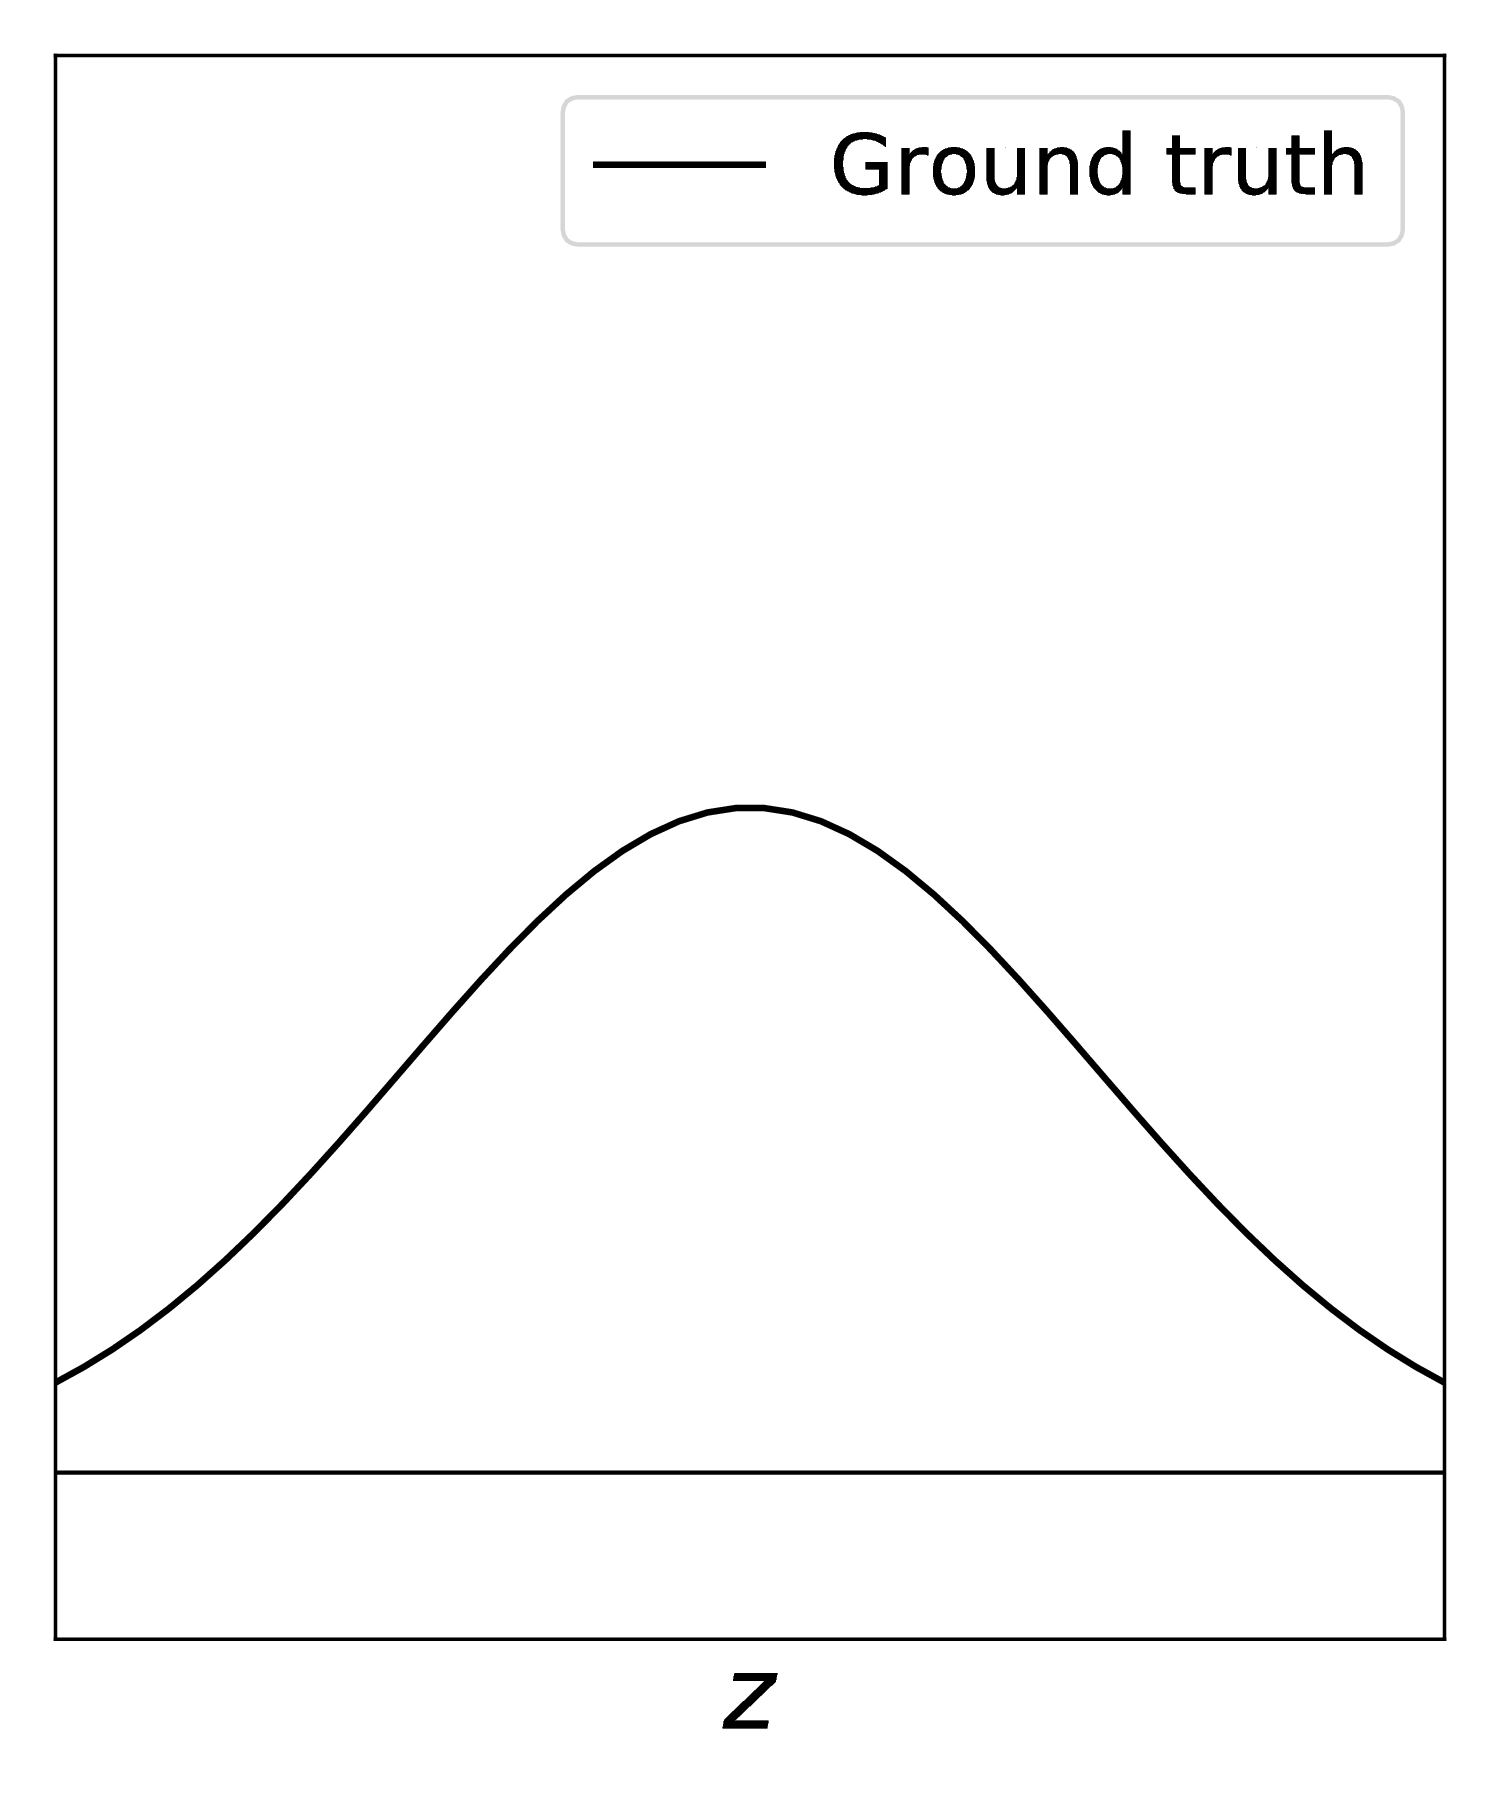
\includegraphics[width=\linewidth]{img/ae_demo_ground.pdf}
\end{subfigure}
\begin{subfigure}{0.22\textwidth}
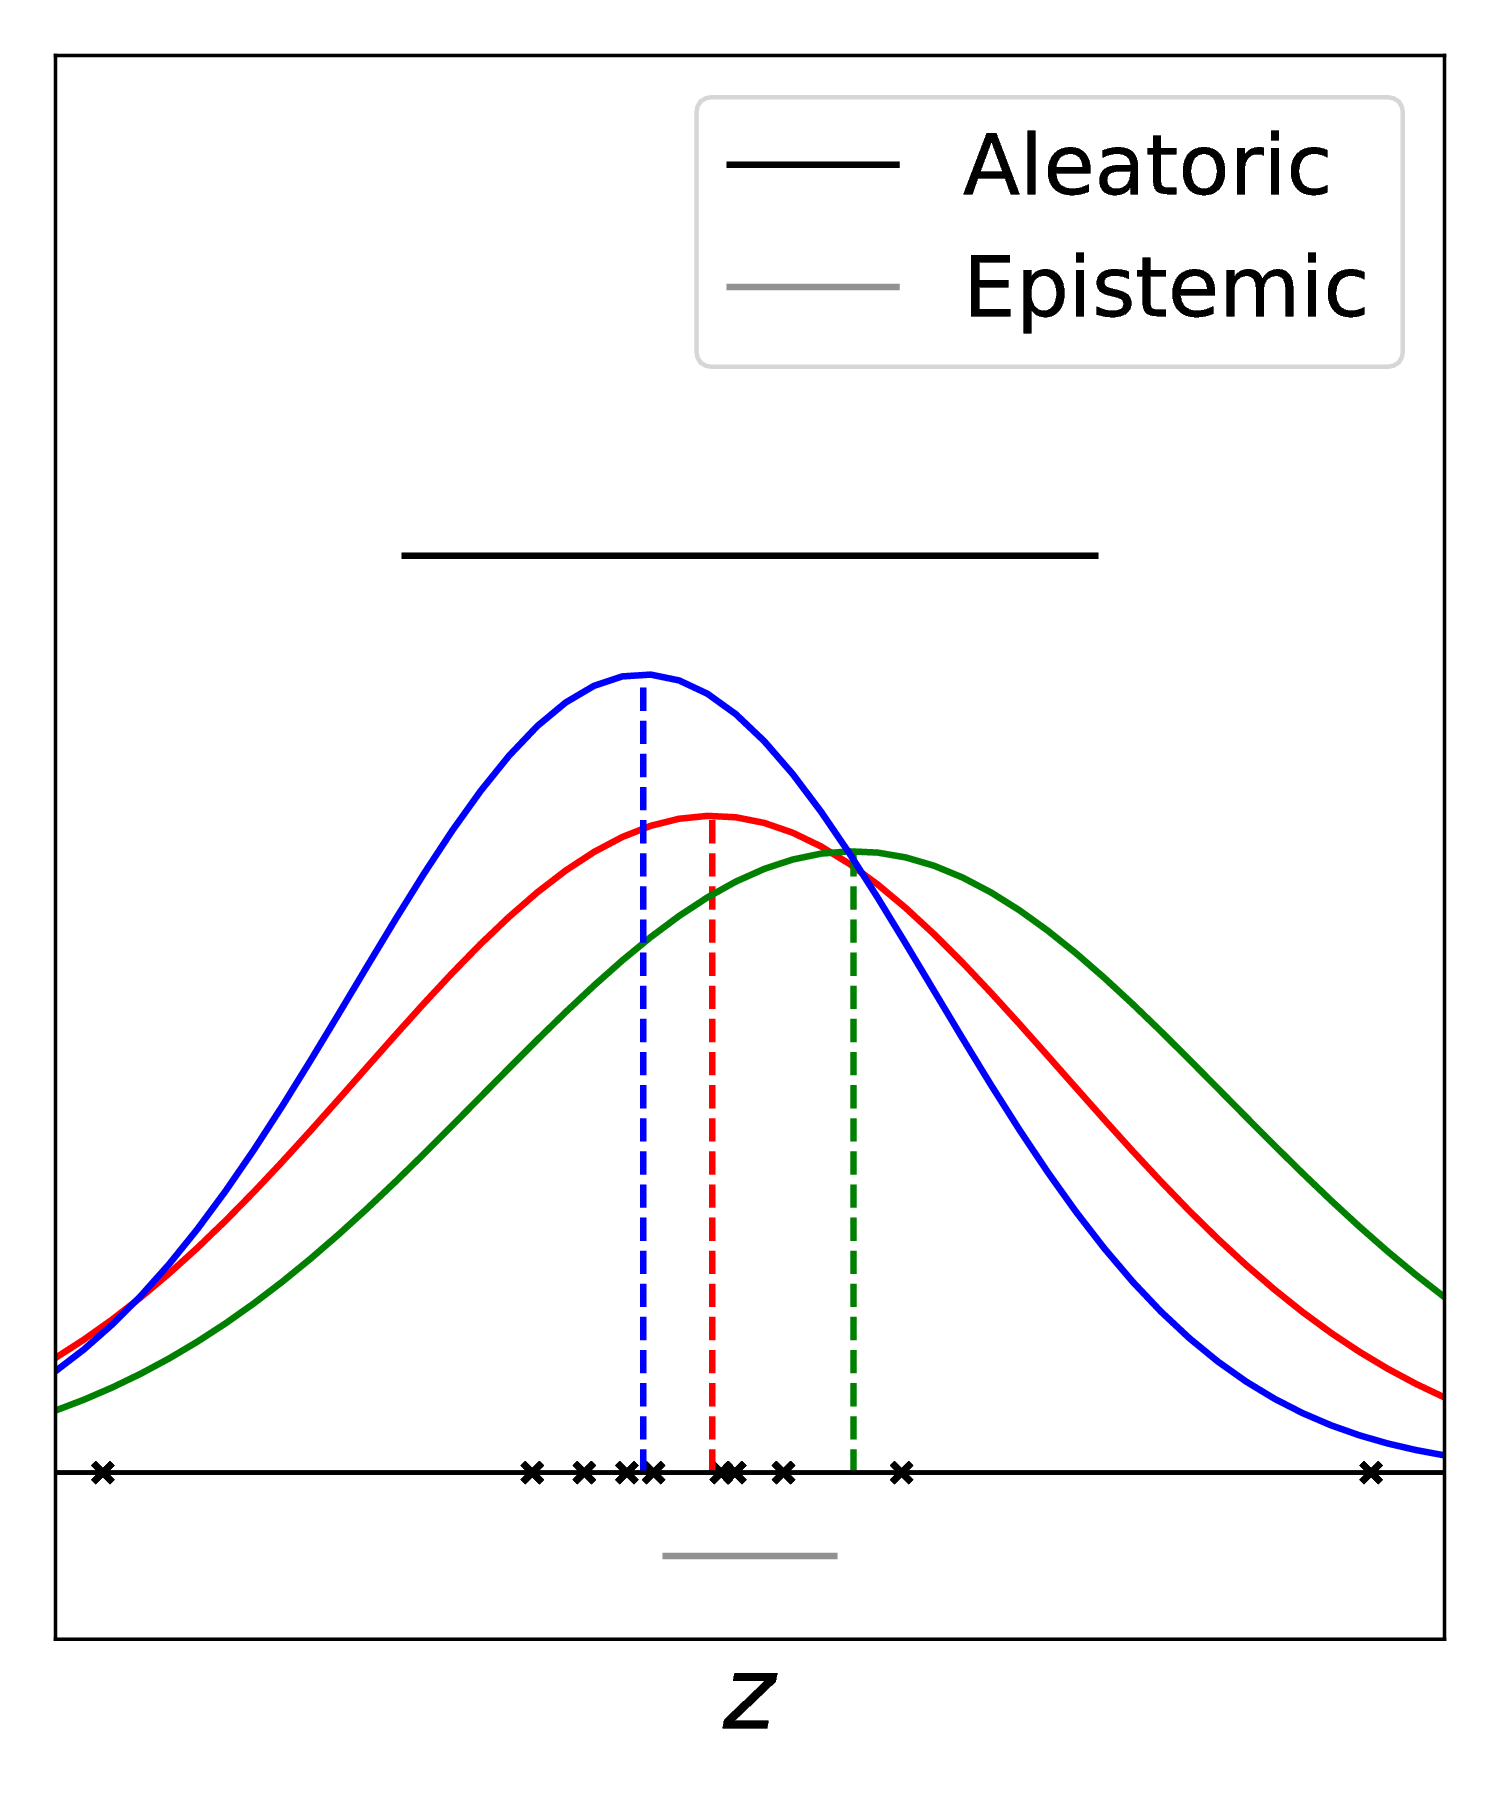
\includegraphics[width=\linewidth]{img/ae_demo_10.pdf}
\end{subfigure}
\begin{subfigure}{0.22\textwidth}
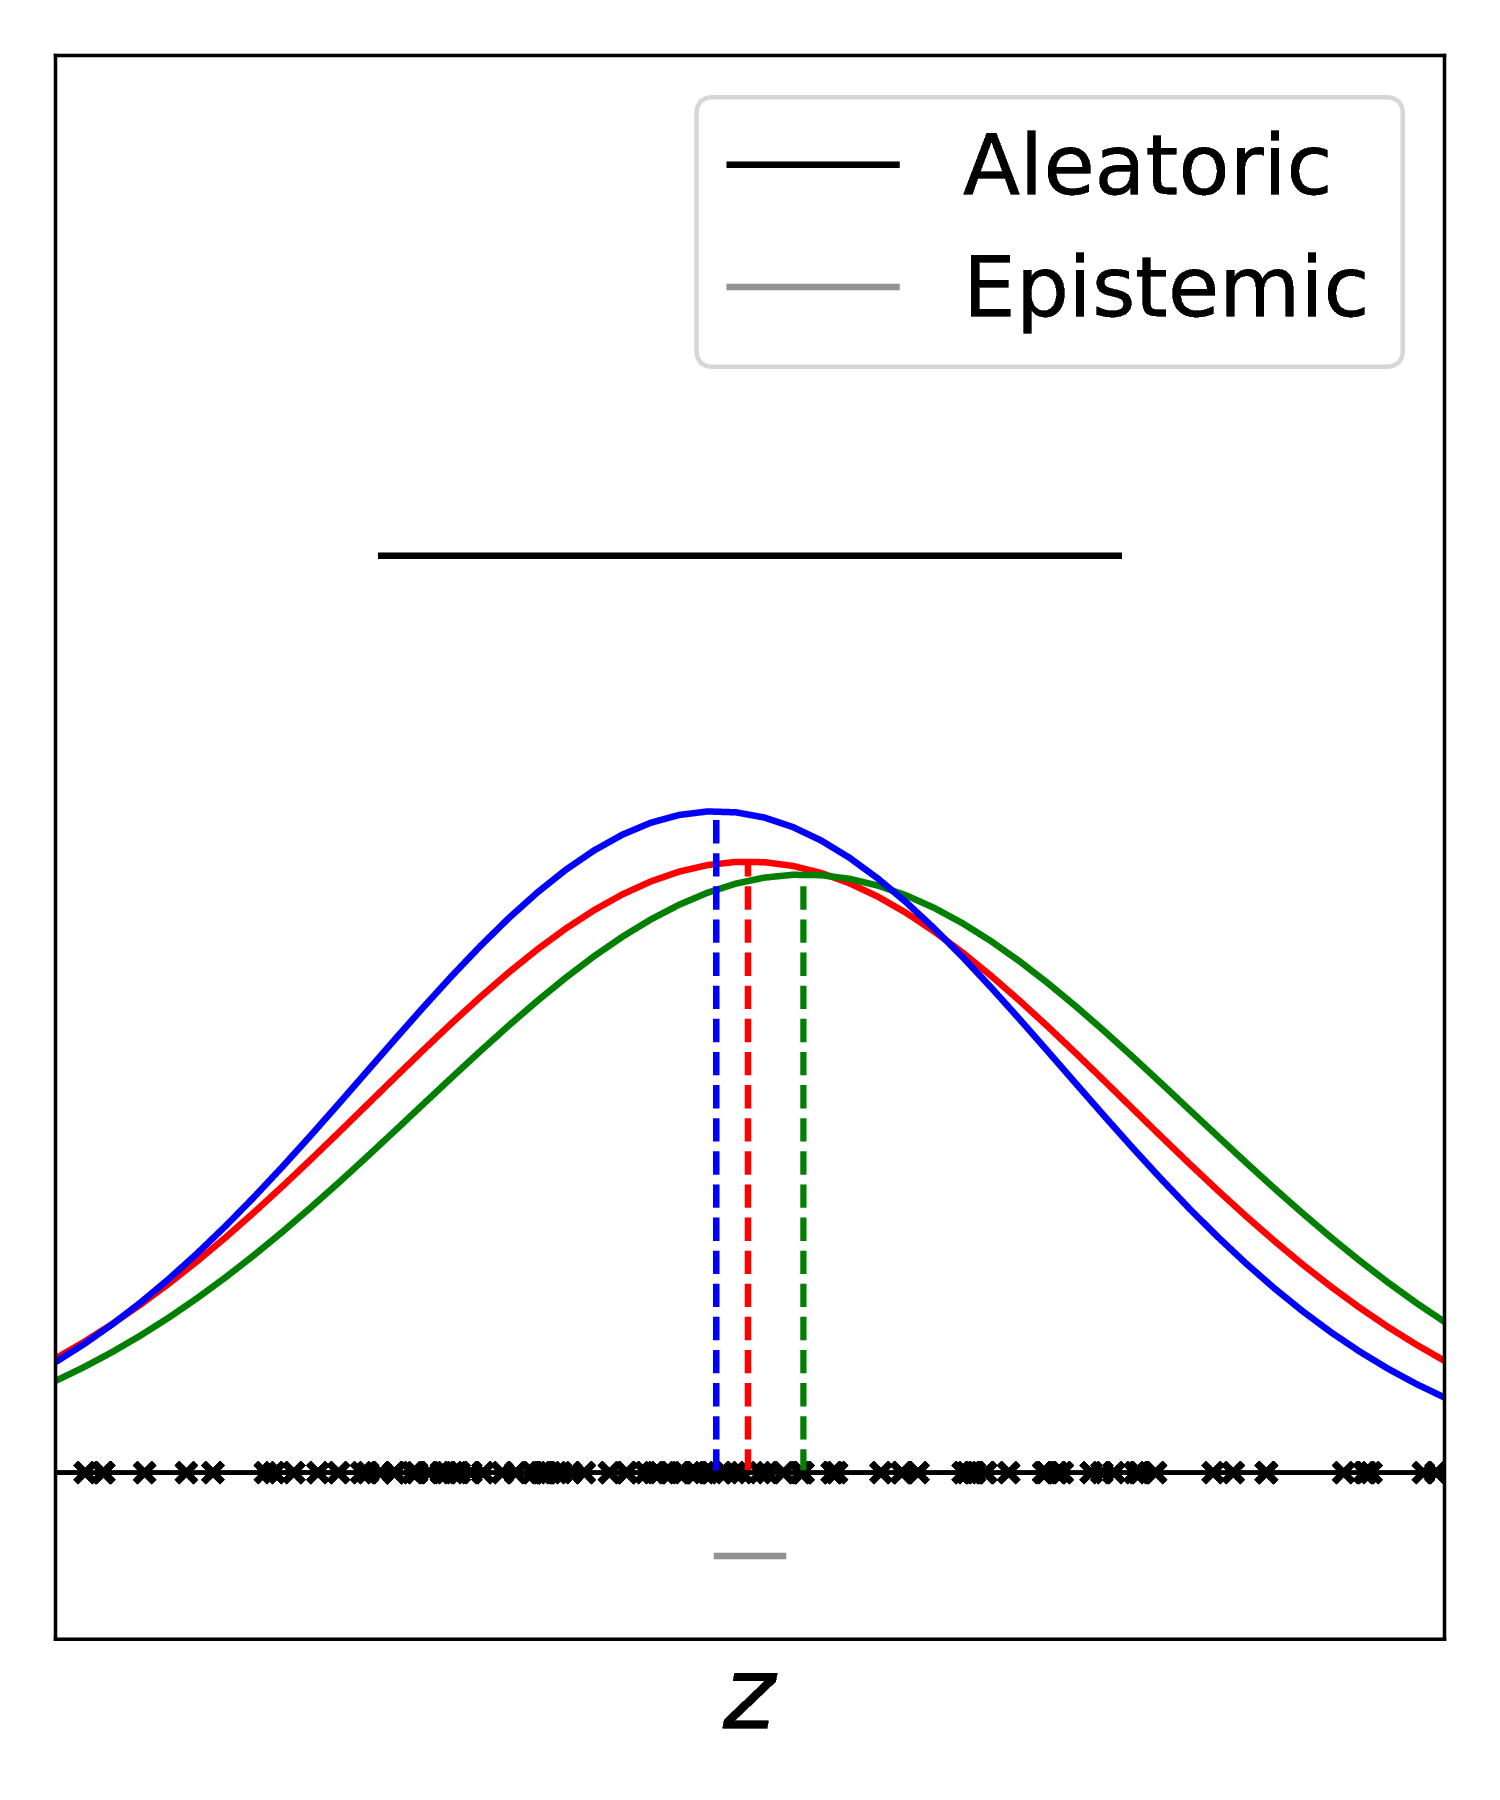
\includegraphics[width=\linewidth]{img/ae_demo_100.pdf}
\end{subfigure}
\captionsetup{width=0.9\linewidth}
\caption{Distinction between aleatoric and epistemic uncertainty for a toy example. As more data are observed (black crosses), the range of plausible Gaussian models narrows down to the ground truth. The epistemic uncertainty in the mean (grey) shrinks, but the aleatoric uncertainty (black) does not reduce bellow the level of inherent noise.}\label{ae_demo}
\end{figure}

Instead, the quantity relevant to exploration is the uncertainty in the parameterisation of $\mczo$ due to the finite amount data, known as the \textit{epistemic} uncertainty - see \cref{ae_demo}. In the limit of zero epistemic uncertainty, the agent is certain about the parameters of its models of $\mct$ and $\mcr$, so acting greedily is optimal given the current data and models - even though there is still aleatoric uncertainty. If the epistemic uncertainty is non-zero, the agent will be uncertain about the \textit{expected returns} and should account for this while exploring. A principled approach would therefore be to quantify the epistemic uncertainty and use it to direct the exploration, e.g. by Thompson sampling \citep{thompson}. This also provides an automatic transition into exploitation, as the posteriors become narrower.

\subsection{Bayes' rule and conjugate priors}

In both the model-based and model-free settings, we are interested in representing the agent's posterior beliefs about $\mct$, $\mcr$, $\mcw$ or $\mcz$. We parameterise relevant distributions by $\btheta$ and then, given data $\data = \{\s, \ac, \ns, r\}$ and a prior $p(\btheta)$, we compute the posterior belief $p(\btheta | \data)$ through Bayes' rule:
\begin{align}
p(\btheta | \data) = \frac{p(\data | \btheta) p(\btheta)}{p(\data)}.
\end{align}
Choosing a \textit{conjugate} prior simplifies downstream calculations: for discrete distributions such as $\mct$, we use a Categorical-Dirichlet model \citep{bishop} for each $(\s, \ac)$, while for continuous distributions such as $\mcr, \mcw, \mcz$ we use a Normal-Gamma (NG) model \citep{murphy} for each $(\s, \ac, \ns)$.


\section{Bayesian RL algorithms}
\subsection{Bayesian Q-Learning}
Bayesian Q-Learning (BQL) \citep{bqlearning} is a model-free algorithm for the tabular setting. The agent models $\mczo$, the distribution over action-returns under $\pi^*$, and updates $p(\thetamczo | \data)$ as data arrive, using a heuristic update rule. The authors make the additional modelling assumptions: (1) the return from any state-action is Gaussian; (2) the prior over the mean and precision for each of these Gaussians is Normal-Gamma (NG); (3) the NG posterior\footnote{Since $\zob$ is modelled by a Gaussian with an NG prior over its mean and precision, the posterior is also NG.} factors over different state-actions.

Although the first two are mild assumptions, the latter is more significant because it approximates the exact posterior by a factored distribution. In reality, the expected returns are related though the BE, so the exact posterior is not factored. See appendix \ref{app:bql} for further details.

\subsection{Posterior sampling for reinforcement learning}

Posterior Sampling for Reinforcement Learning (PSRL) \citep{psrl} is an elegantly simple and yet provably efficient model-based algorithm for sampling from the exact posterior over optimal policies $p(\pi^* | \data)$. It amounts to sampling $\thetamcthat \sim \thetamctpost$ and $\thetamcrhat \sim \thetamcrpost$, and solving the BE for $\hat{Q}^* | \thetamcthat, \thetamcrhat $ and $\hat{\pi}^* | \thetamcthat, \thetamcrhat$. Policy $\hat{\pi}^*$ is then followed for a single episode, or for a pre-defined horizon in continuing tasks. See appendix \ref{app:psrl} for further details.

\subsection{The uncertainty Bellman equation}
The Uncertainty Bellman Equation (UBE), is a model-based method proposed by \cite{ube}, for estimating the epistemic uncertainty in $\mu_{\zb} = \E_z [\zb | \thetamcz]$. The authors assume that: (1) the MDP is a directed acyclic graph (DAG) and the task is episodic with time variable $t = 1, ..., T$; (2) the mean rewards of the MDP are bounded within $[-R_{max}, R_{max}]$. Taking variances across the BE and defining an appropriate Bellman operator, they show that corresponding UBE has a unique solution $u_{\s, \ac, t}^\pi$ which upper bounds the epistemic uncertainty $\Var_{\thetamct, \thetamcr} \big[ \mu_{z^{\pi}_{\s, \ac, t}} \big]$.

In practice, assumption (1) must be violated to apply the UBE to non-DAG MDPs or in the continuing setting. Solving for the greedy policy ${\pi^*} | \thetamct, \thetamcr$ and then for $u_{\s, \ac}^{*}$, Thompson sampling can be performed from a diagonal Gaussian - leading to a factored posterior approximation. The Thompson noise is scaled by an appropriate scaling factor, $\zeta$. Further details are given in appendix \ref{app:ube}.

\subsection{Moment matching across the Bellman equation}

Our moment matching (MM) approach uses the BE to estimate epistemic uncertainties, without resorting to computation of an upper bound. Instead, we require equality of first and second moments across the BE. The first-order equation gives the familiar BEs for $\V$ and $\Q$. Using the laws of total variance and covariance \citep{weiss}, the second-order moments can be decomposed into purely aleatoric and purely epistemic terms which, we argue, should satisfy two separate equations.

We thus propose first solving for the greedy policy $\pi^*$ w.r.t. $p(\thetamct | \data)$ and $p(\thetamcr | \data)$, and then for the epistemic uncertainty in $\mu_{z^*_{\s, \ac}}$. The latter is used for Thompson sampling from a diagonal Gaussian - also yielding a factored approximation. Further details are given in appendix \ref{app:mm}.

\section{Environments and methods}

We compare the algorithms on finite MDPs of various sizes in the continuing setting, measuring performance by the cumulative regret to an oracle-agent following the optimal policy\footnote{Our implementations and plotting code can be found at \scriptsize{\texttt{\href{https://github.com/sample-efficient-bayesian-rl/nips-2019-rl-workshop}{https://github.com/sample-efficient-bayesian-rl}}}.} - see appendix \ref{app:env} for details. Our DeepSea MDP, a variant of that in \cite{deepsea}, tests the algorithm's ability for sustained exploration. We propose the WideNarrow environment for investigating the effect of factored posterior approximations. Finally, we compare the algorithms on random MDPs, with dynamics and rewards drawn from Categorical and NG priors as in \cite{psrl} - we refer to this as PriorMDP.

\section{Results and discussion}

We observe several trends in our results. \Cref{combined_regret_summary} shows the regret, normalised by cumulative reward received by the oracle, to make the performances comparable on the same scale - see appendix \ref{app:supfig} for further results and supporting figures.
\begin{figure}[h!]
\centering
\begin{subfigure}{1.\textwidth}
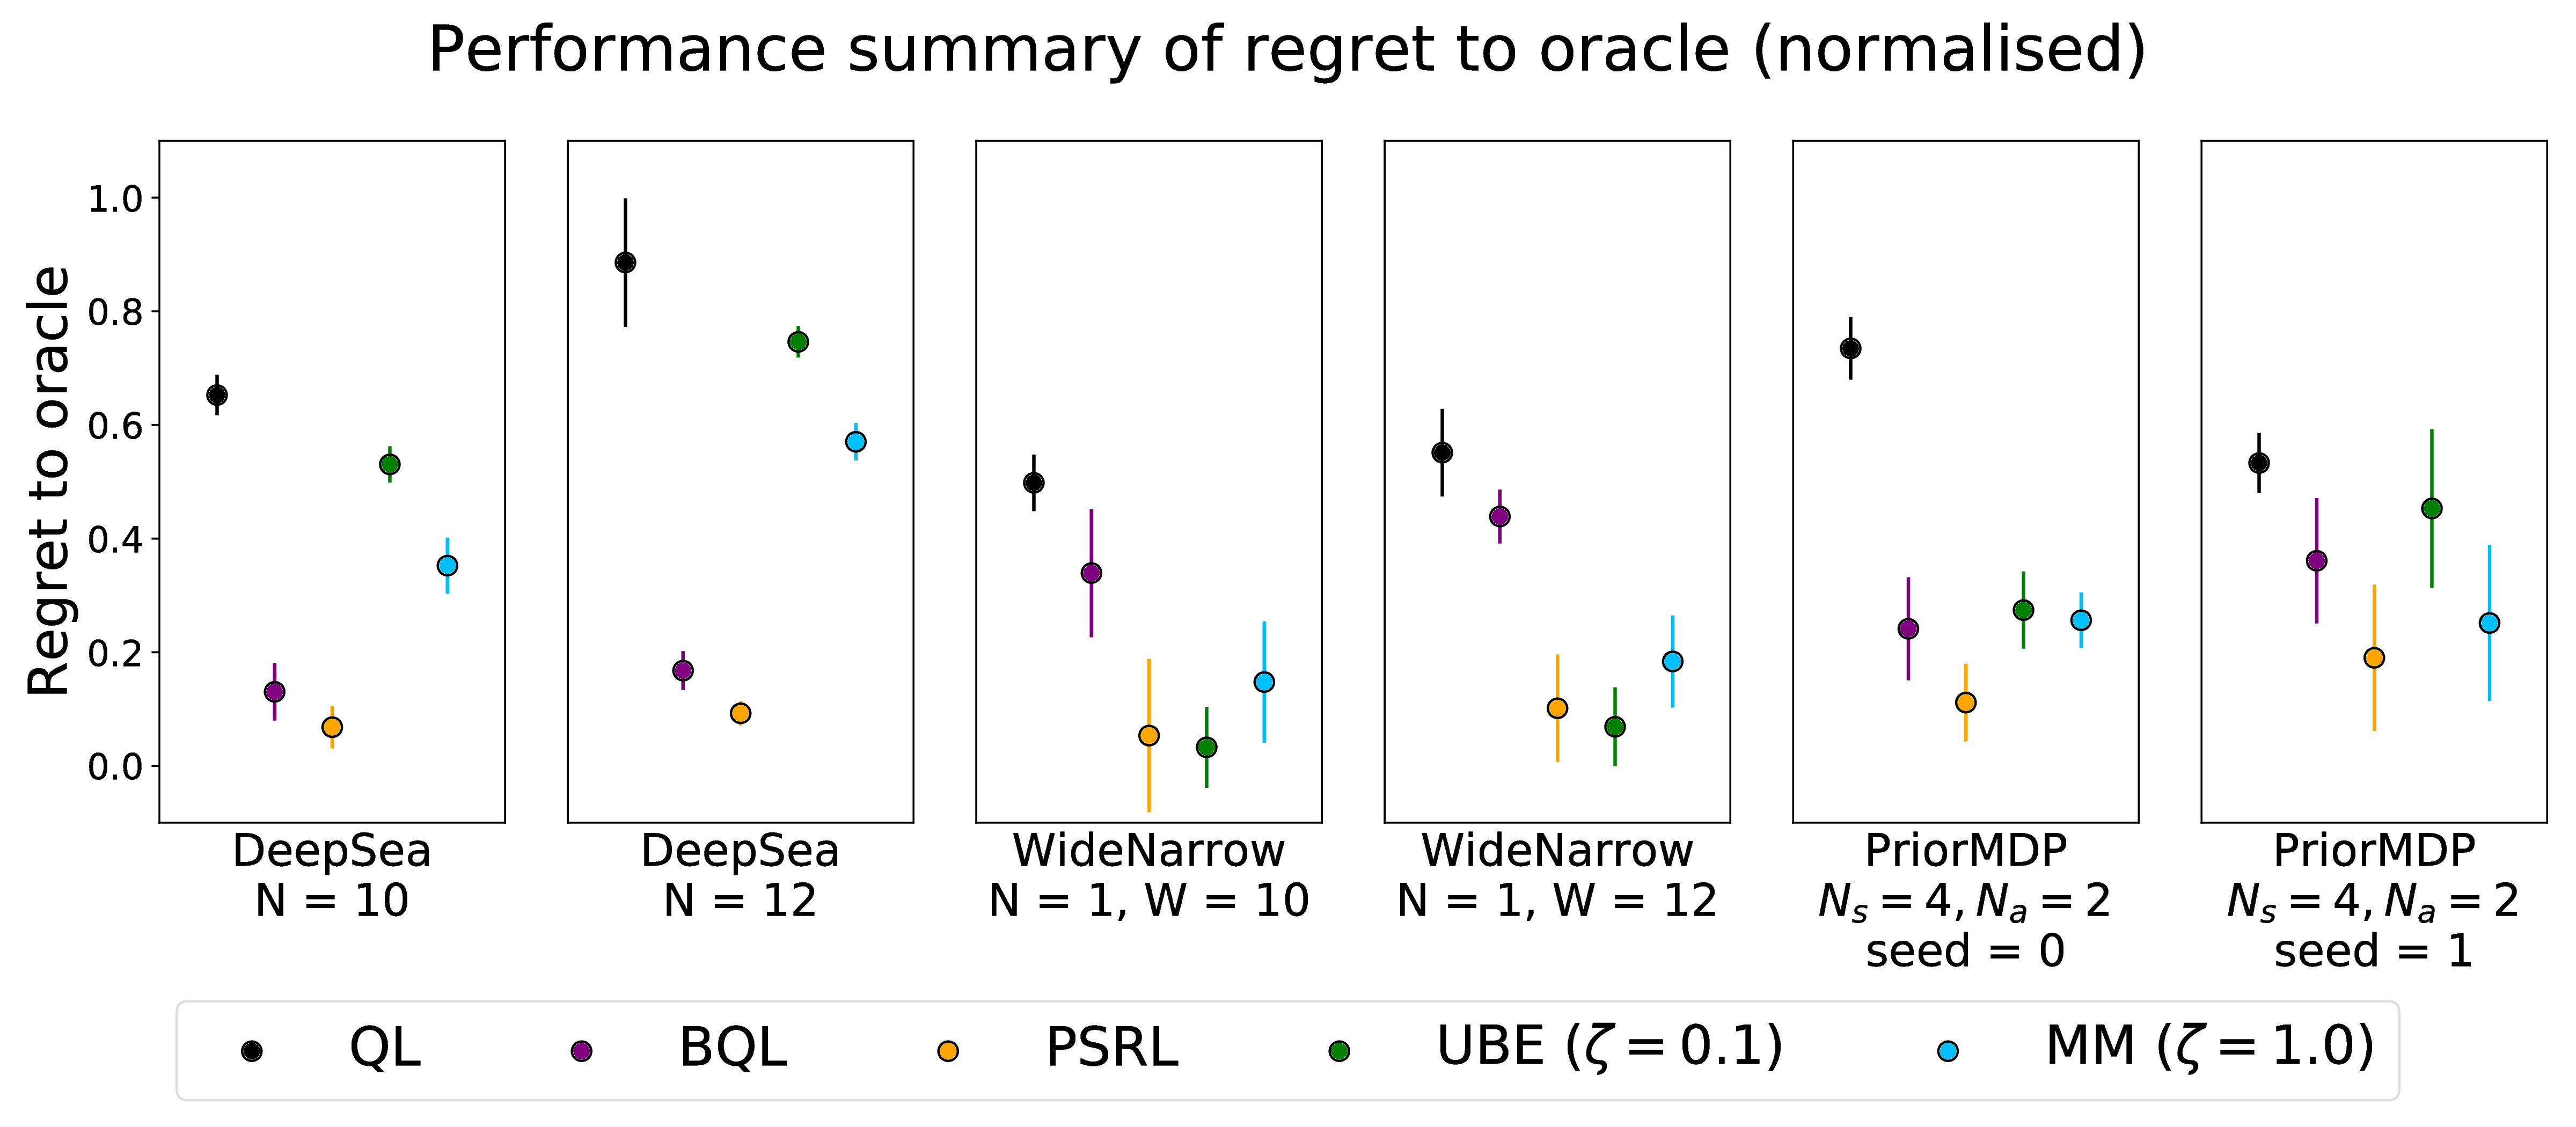
\includegraphics[width=\linewidth]{img/regret_combined.pdf}
\end{subfigure}
\captionsetup{width=0.9\linewidth}
\caption{Summary performances in terms of regret to the oracle on selected environments. $N$, $W$, $N_s$ and $N_a$ are environment size parameters - see \cref{app:env} for specifications.}\label{combined_regret_summary}
\end{figure}
\begin{figure}[h!]
\centering
\begin{subfigure}{0.49\textwidth}
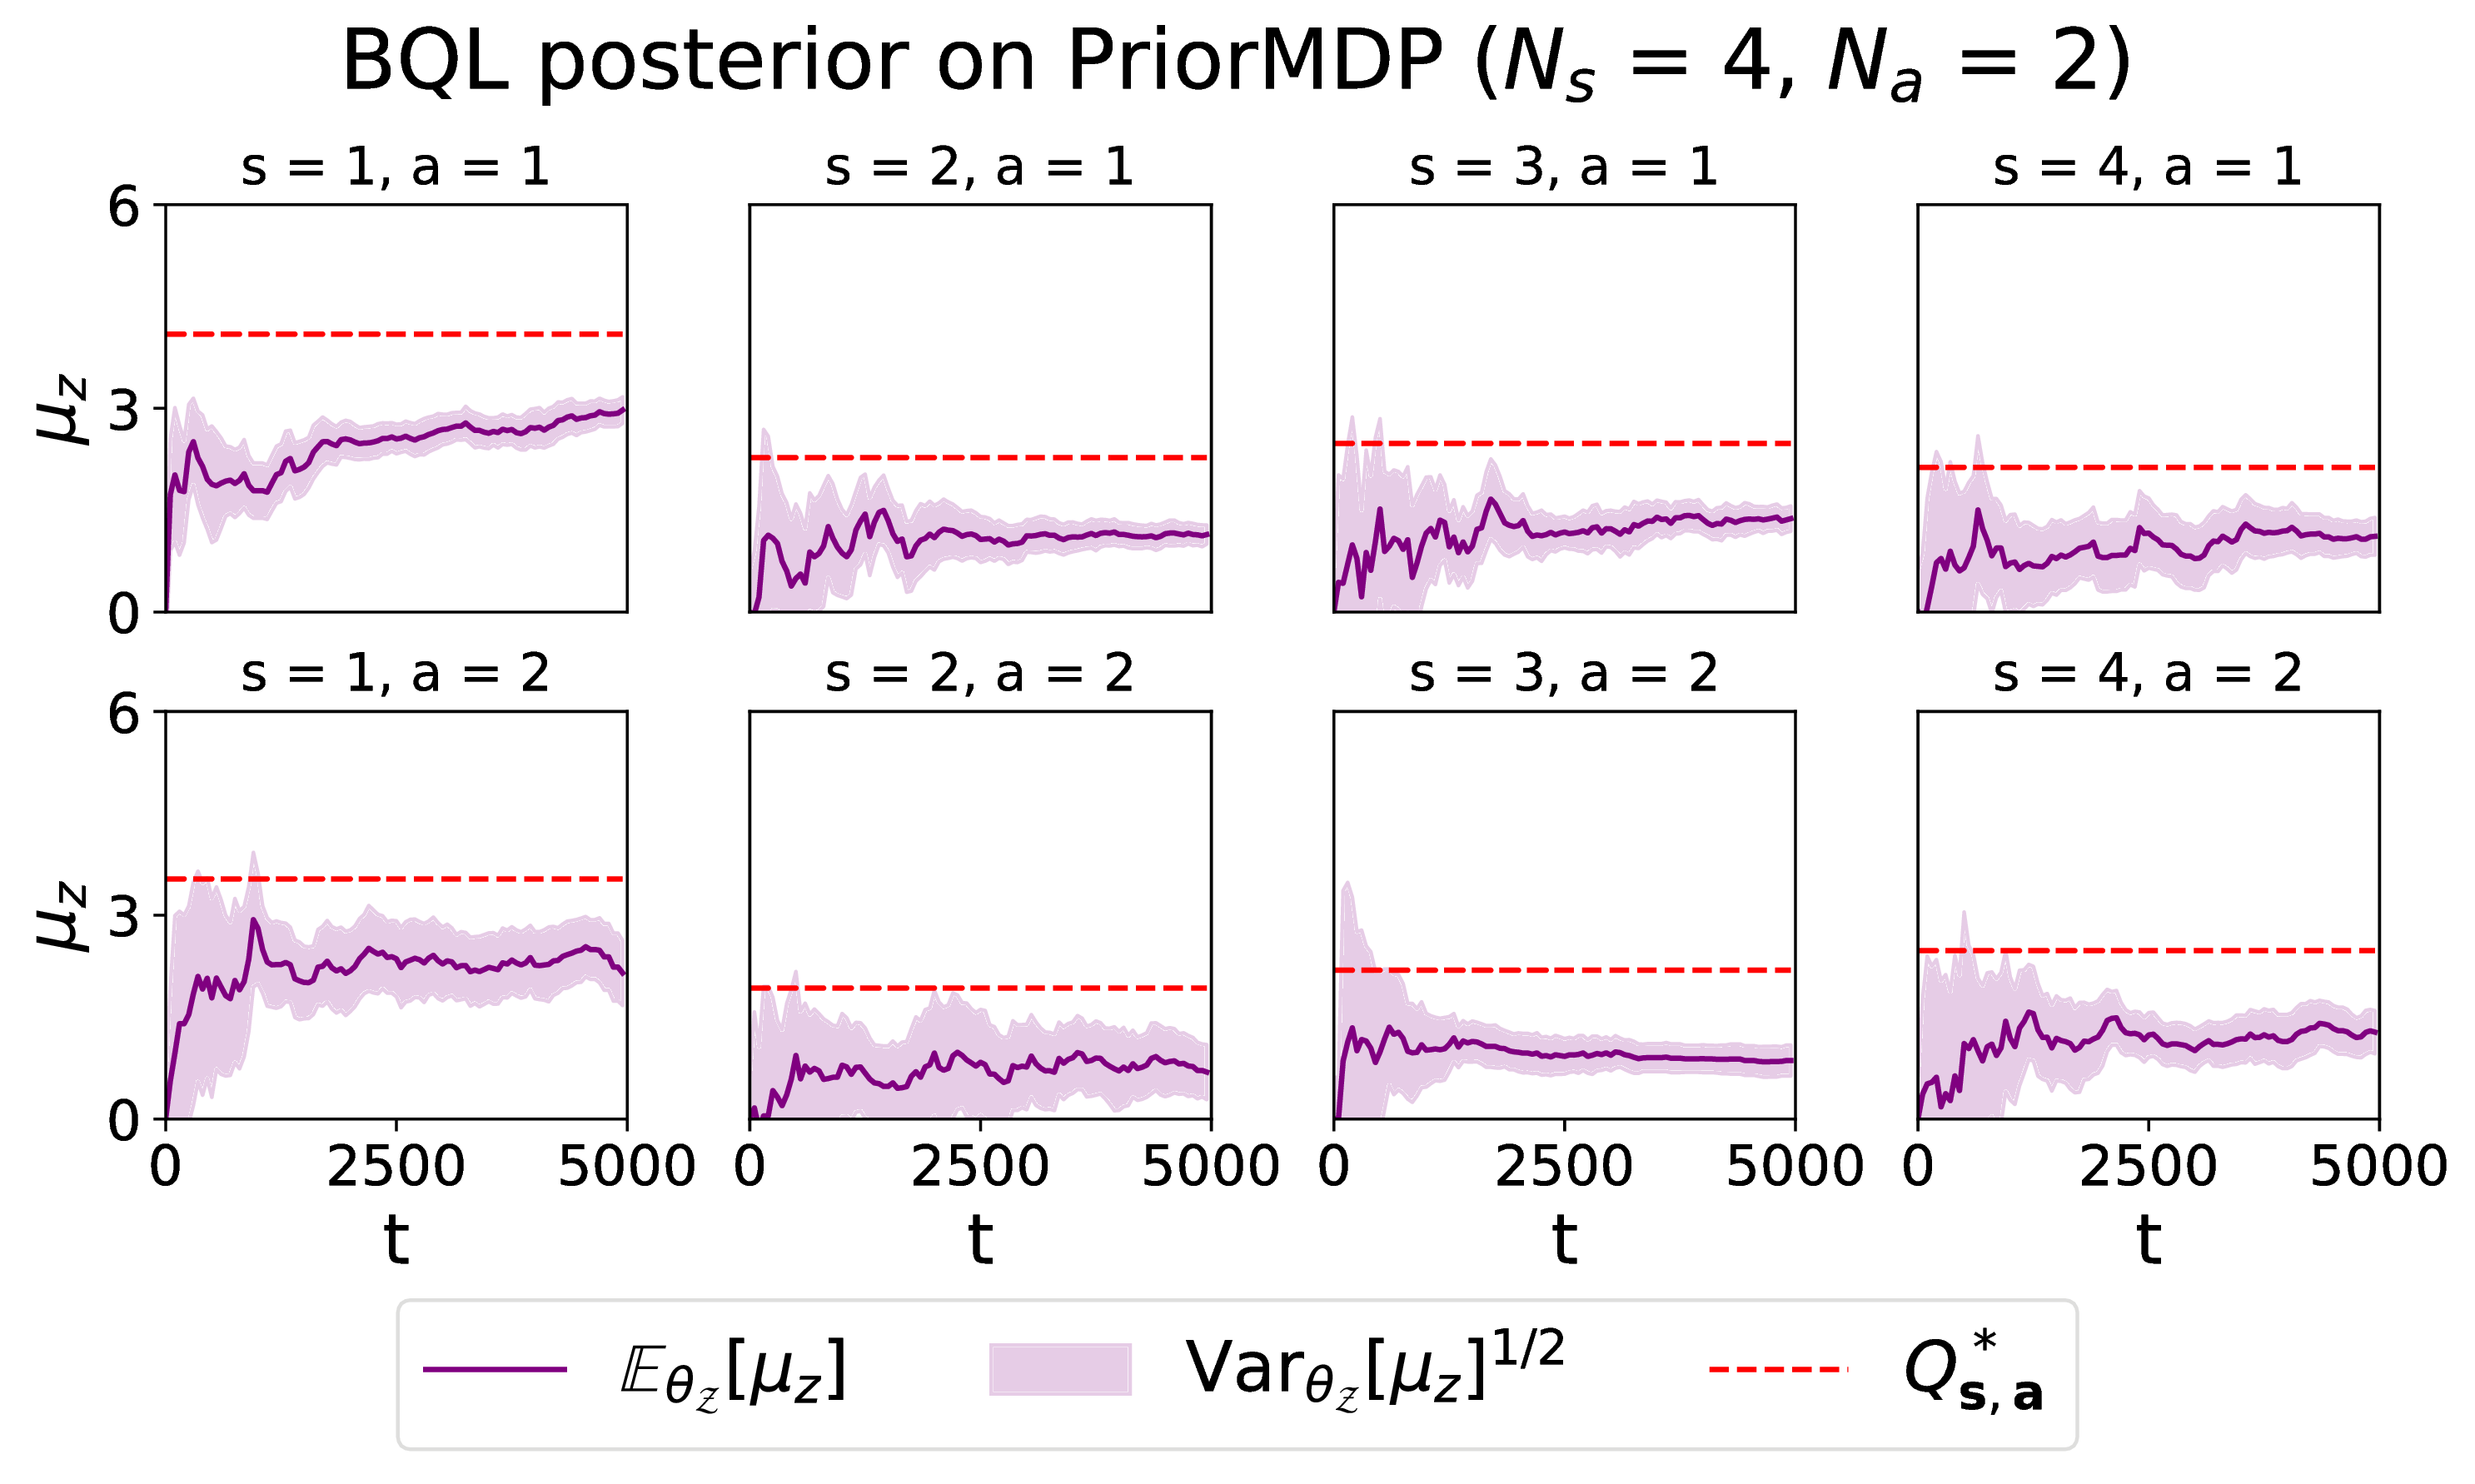
\includegraphics[width=\linewidth]{img/bql-0_0-4_0-3_0-3_0-posterior-priormdp-4-2-seed-0.pdf}
\end{subfigure}
\begin{subfigure}{0.49\textwidth}
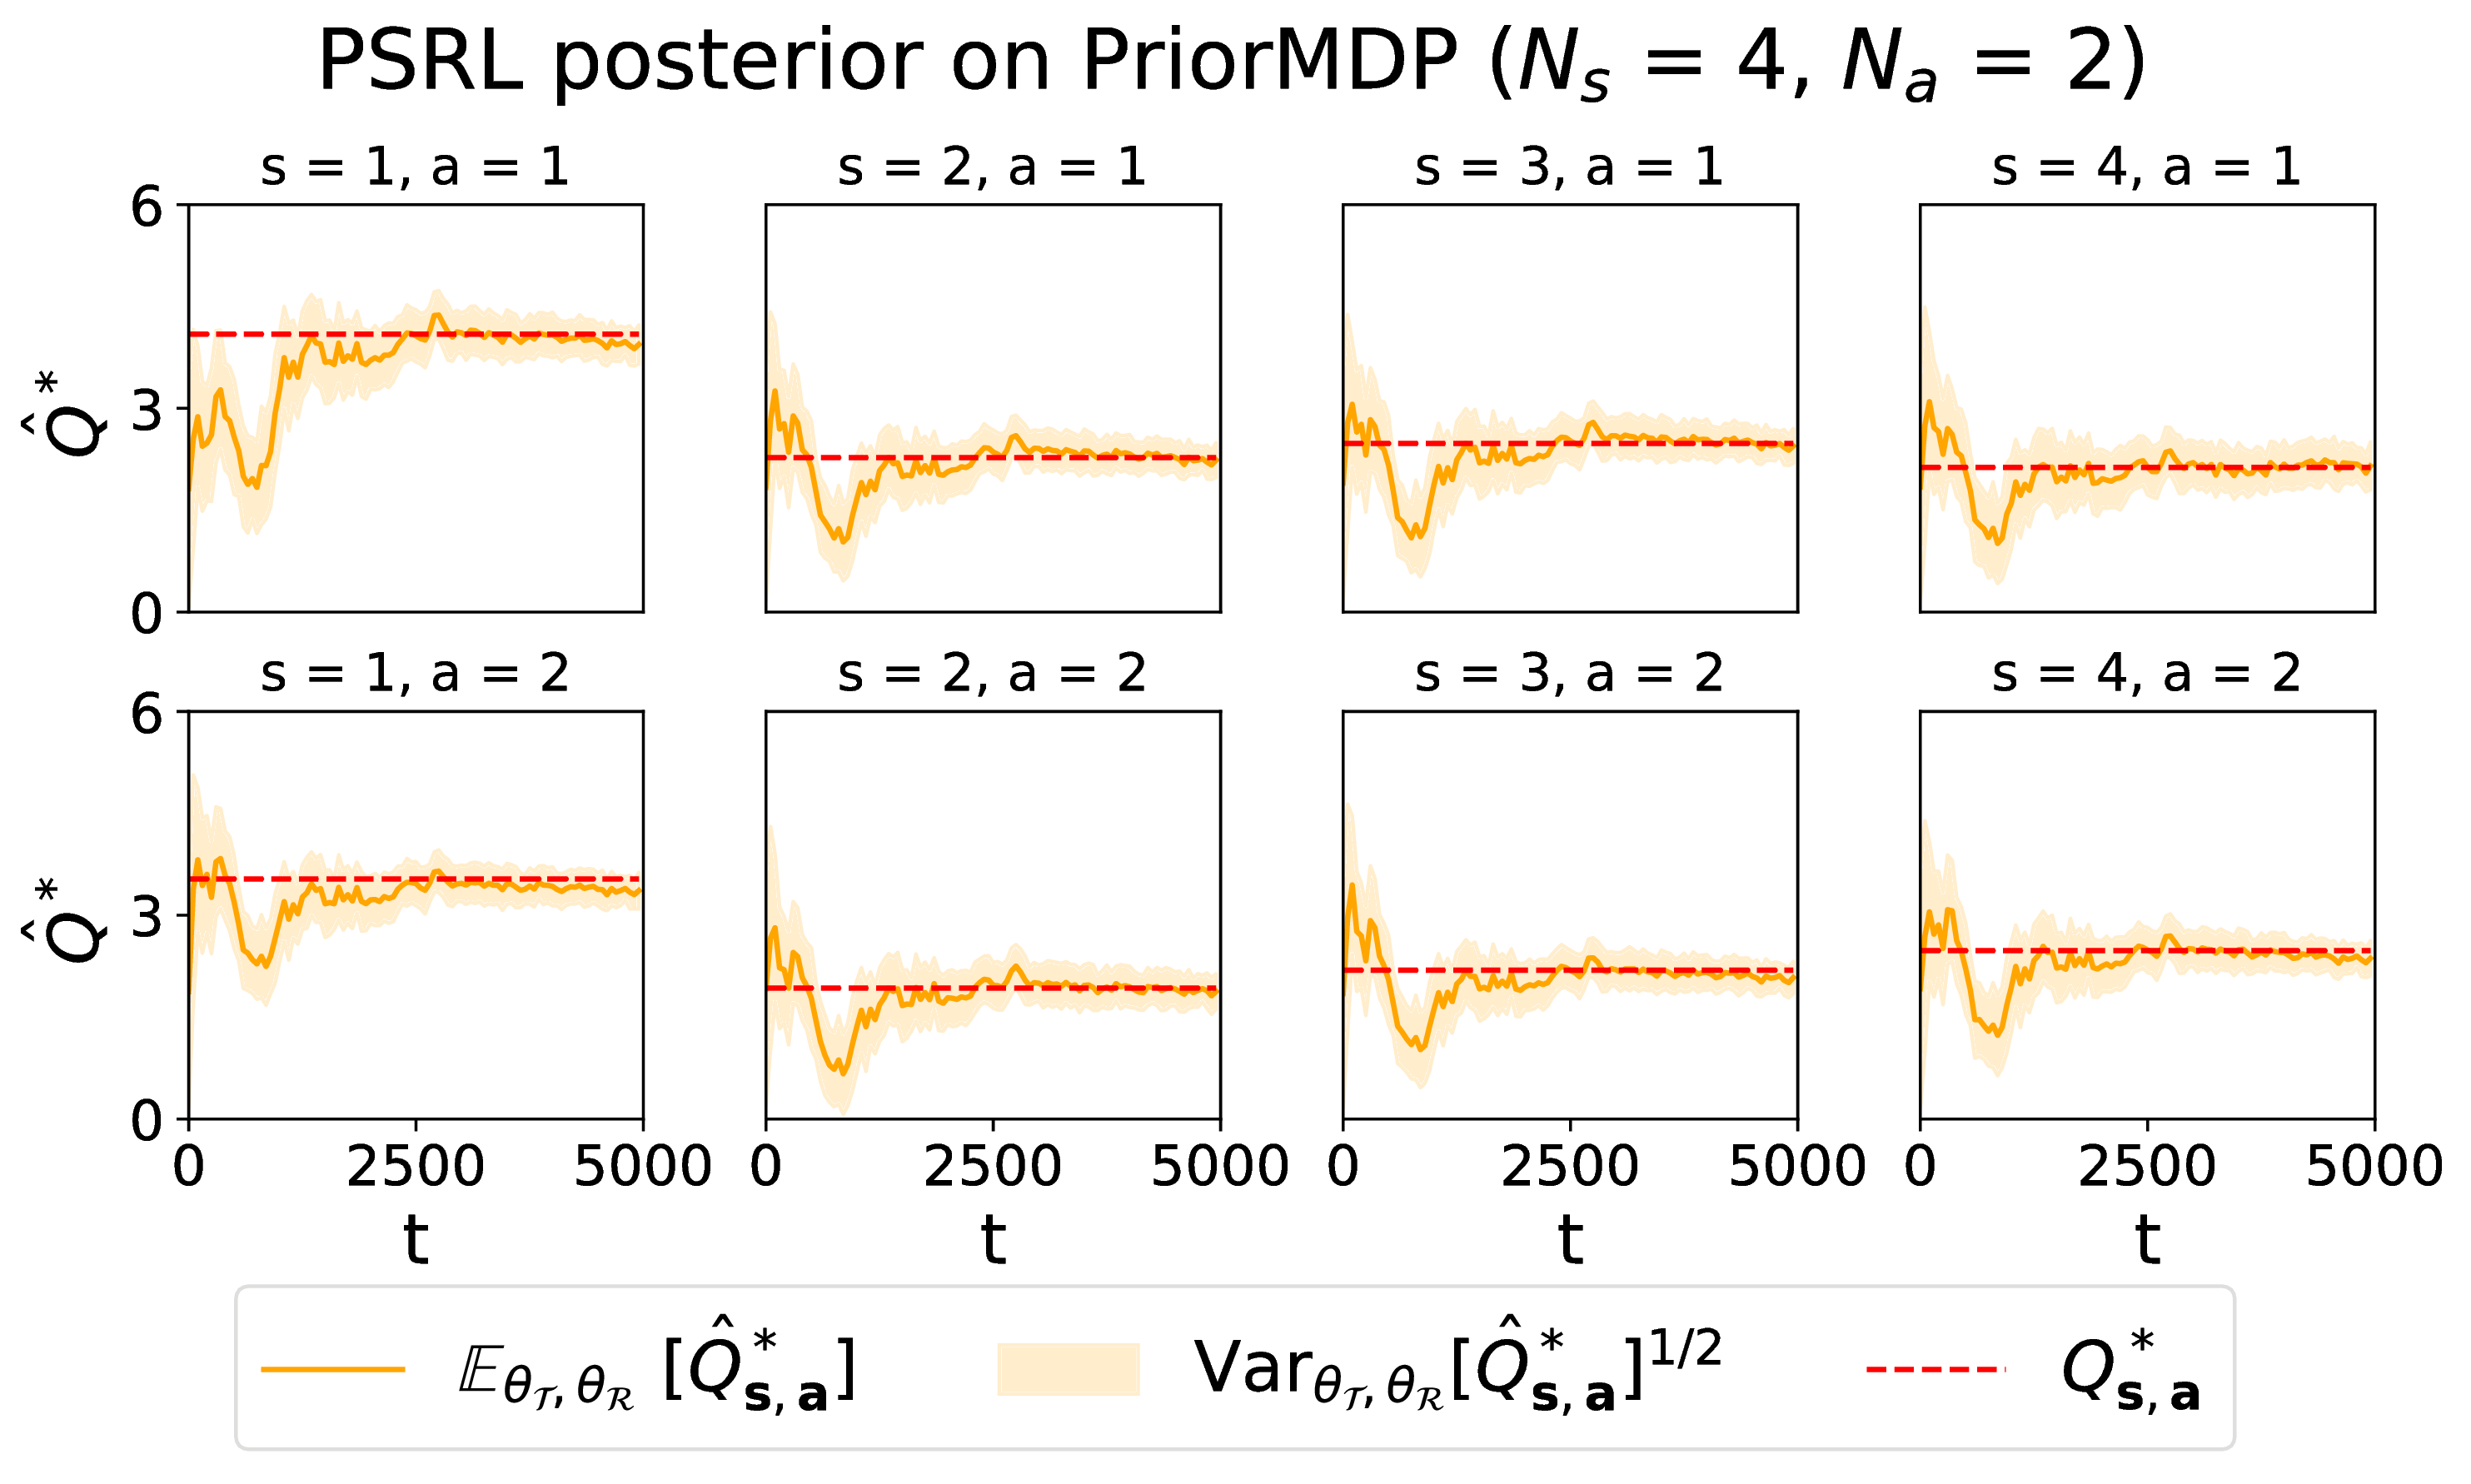
\includegraphics[width=\linewidth]{img/psrl-0_0-4_0-3_0-3_0-posterior-priormdp-4-2-seed-0.pdf}
\end{subfigure}
\begin{subfigure}{0.49\textwidth}
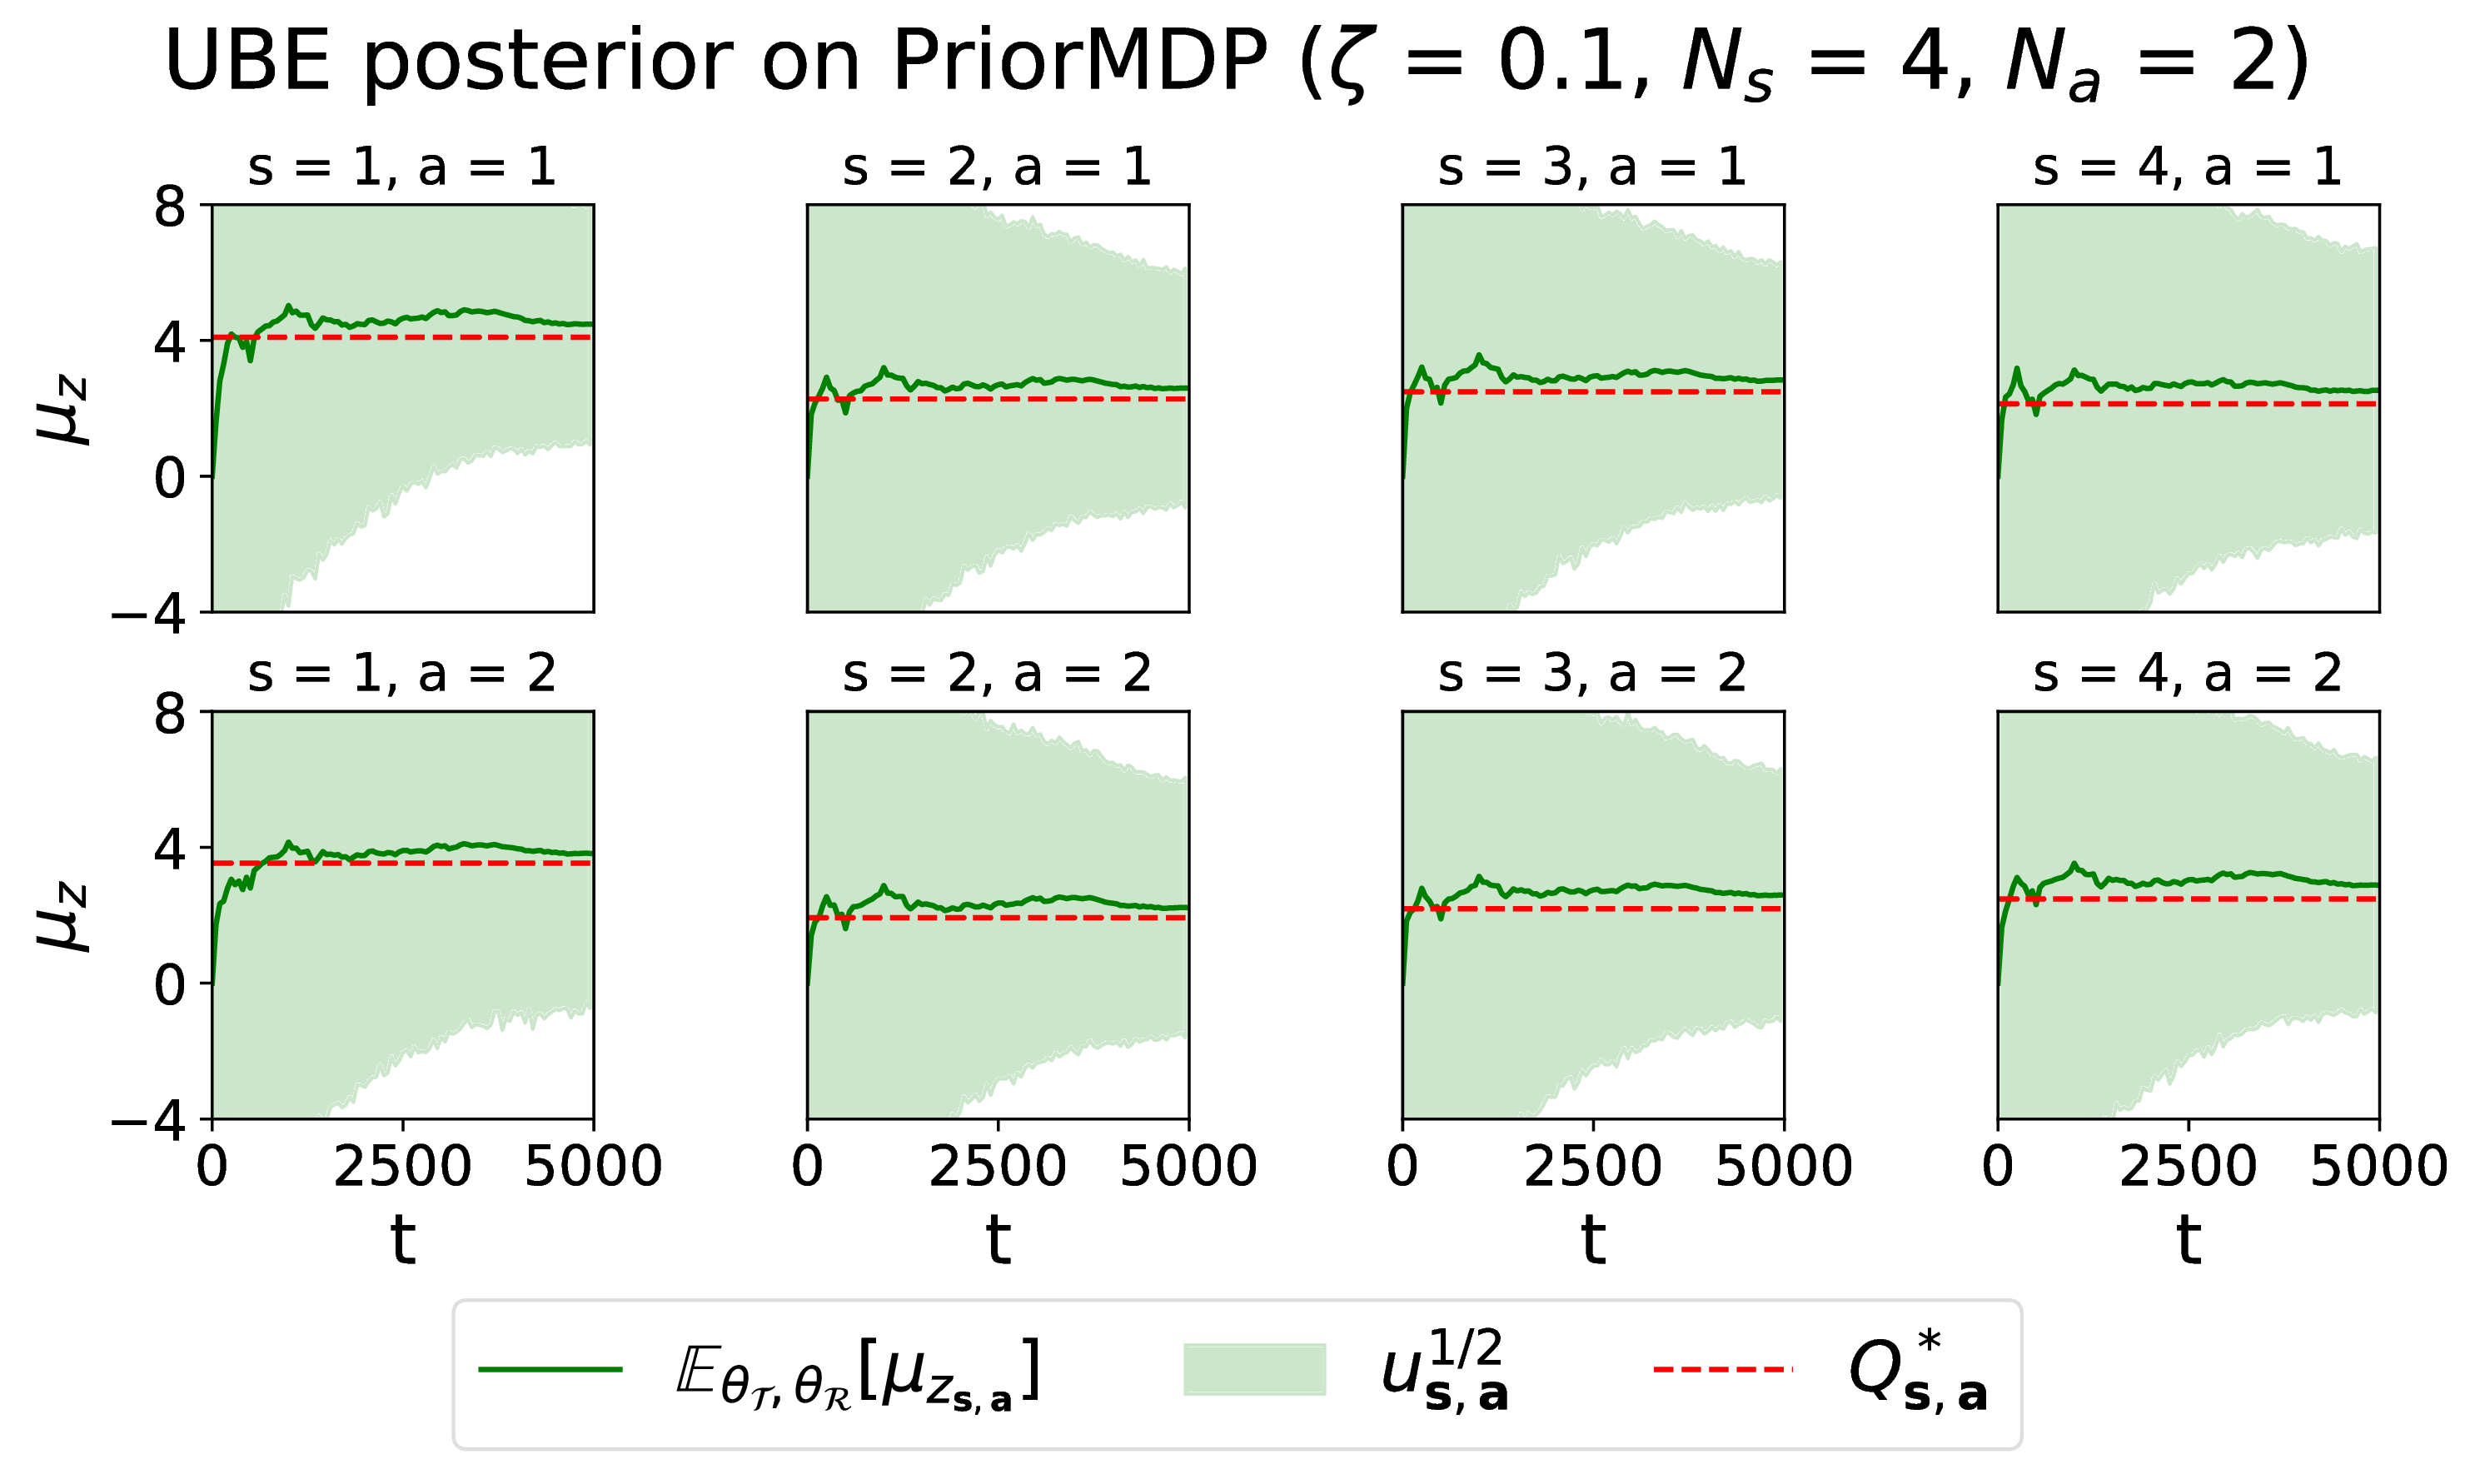
\includegraphics[width=\linewidth]{img/ube-0_0-4_0-3_0-3_0-0_1-posterior-priormdp-4-2-seed-0.pdf}
\end{subfigure}
\begin{subfigure}{0.49\textwidth}
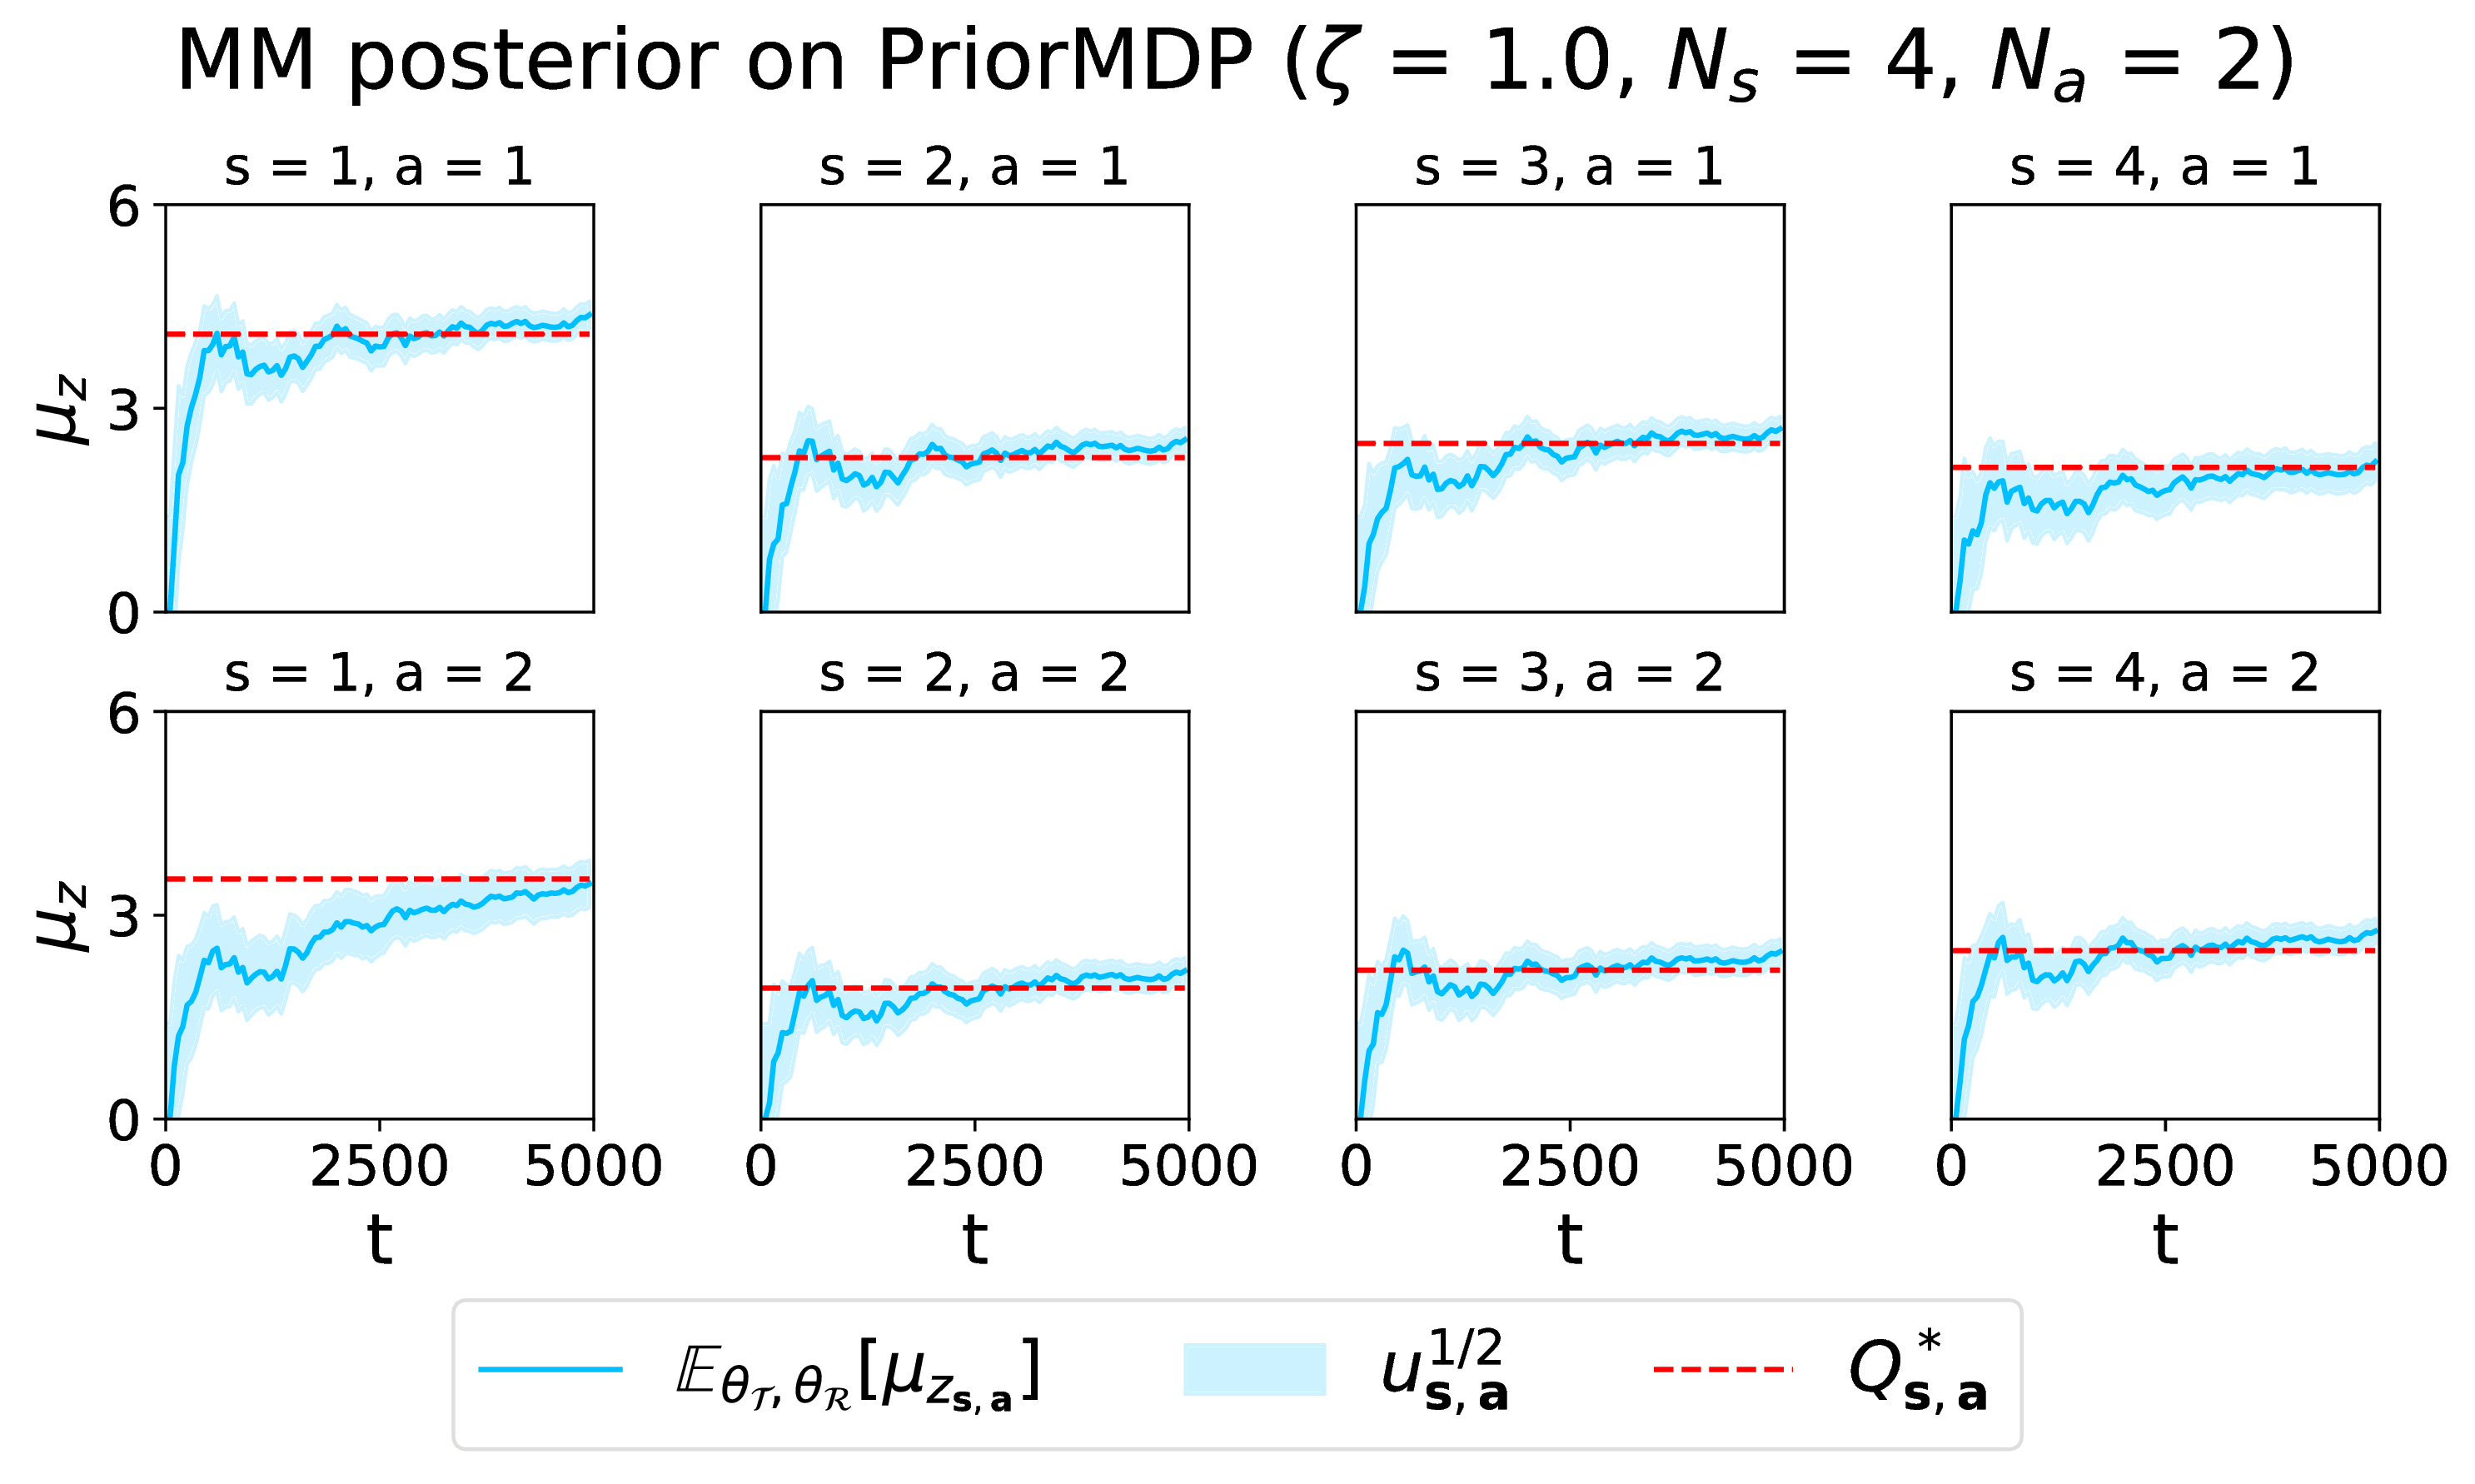
\includegraphics[width=\linewidth]{img/mm-0_0-4_0-3_0-3_0-1_0-posterior-priormdp-4-2-seed-0.pdf}
\end{subfigure}
\captionsetup{width=0.9\linewidth}
\caption{Plots of the evolution of the posterior on the same PriorMDP for each algorithm.}\label{combined_posterior_evolution}
\end{figure}
\Cref{combined_posterior_evolution} shows the evolution of the posterior of each algorithm on a PriorMDP during learning. Generally, as training progresses the posteriors concentrate on the true $Q^*$ values, the behaviour policy converges on the optimal one and the agent smoothly transitions into greedy action selection. Often, the agent does not over-explore actions if it is confident that these are suboptimal. For example, this is seen for BQL, $(\s = 1, \ac = 1)$, in \cref{combined_posterior_evolution} - see also \cref{bql_deepsea_visual} and \cref{psrl_deepsea_visual}. Although there is significant uncertainty in the $\mu_{\zob}$ of the suboptimal action, the agent is confident that the optimal action ($\ac = 1$) is better. It therefore does not waste time determining the exact $\mu_{\zob}$ of an action if it is confident that it is suboptimal. The aforementioned behaviours are central for achieving principled and efficient exploration. However we often observe cases where the algorithms depart from these desirable behaviours.

First, the UBE uncertainty estimate $u^*_{\s, \ac}$ remains extremely loose even after a large number of time-steps (\cref{combined_posterior_evolution} and also \cref{ube_deepsea_visual1}, \cref{ube_widenarrow_visual1} and \cref{ube_priormdp_visual1}). Even though $\mu_{\zob}$ be close to $Q^*$, $u^*_{\s, \ac}$ is so large that the Thompson noise completely smooths out differences between actions, which are picked almost uniformly at random. Further, $u^*_{\s, \ac}$ shrinks very slowly and the transition to greedy behaviour takes an extremely long time, causing poor regret performance. These effects are due to the contribution of an extremely large term coming from the upper-bound derivation of \cite{ube} - this is the $Q_{max}$ term in \cref{eq:bellunc} and \cref{eq:localunc}. Further, inspecting contributions to $u^*_{\s, \ac}$ (\cref{ube_unc_terms}), reveals that an upper-bounding contribution from the dynamics uncertainty completely outweighs the rewards uncertainty, which is effectively neglected. Scaling the Thompson noise by $\zeta < 1.0$, improves regret performance in some cases. However, one is further faced by the challenge of tuning $\zeta$, which may be expensive and challenging for large problems. By contrast, MM produces better-calibrated uncertainty estimates than the UBE (\cref{combined_posterior_evolution} and also \cref{mm_deepsea_visual}, \cref{mm_widenarrow_visual} and \cref{mm_priormdp_visual}). As a result, MM shows typically better regret performance than the UBE without a need to tune $\zeta$. This could give an advantage to MM in settings where tuning $\zeta$ may be expensive or difficult.

Second, we observe that the BQL posterior sometimes fails to concentrate on the true $Q^*$ values (\cref{combined_posterior_evolution} and also \cref{bql_deepsea_visual} and \cref{bql_priormdp_visual}), where the posterior is overconfident about incorrect predictions of $\mu_{\zob}$. This effect persists for different random seeds and is affected by the prior used. In particular, using an NG prior with a mean $\mu_0$ that is closer to the true $Q^*$ values, results in the posterior concentrating on $Q^*$. These effects can be explained through the update rule used in BQL (\cref{eq:mixture}). The update rule uses the next-state-action posterior $p(\zonb | \data)$ to update the current state-action posterior. If the former is inaccurate and overconfident, the updated hyperparameters are affected accordingly. BQL can hardly escape from this situation because it does not involve a \textit{forgetting mechanism} for inaccurate updates far in the past. Contrast this with $Q$-Learning, in which the Temporal Difference updates result in forgetting past inaccurate $Q$-estimates. Model-free Bayesian approaches with a rule similar to BQL may suffer from a similar pathology.

Third, there is strong evidence that factored approximations made by BQL, UBE and MM have a significant effect on regret performance. Factored approximations result in overly loose posteriors (see \cref{correlations_widenarrow_500}, \cref{correlations_widenarrow_2500}, \cref{correlations_priormdp_500} and \cref{correlations_priormdp_2500}) and as a result, the Thompson-sampled $\mu_{\zob}$ often correspond to picking a sub-optimal action. By contrast, PSRL draws samples from the exact posterior and thereby accounts for correlations between different state-actions, which are in fact quite significant. The exact posterior often has marginals of similar scale as those of BQL or MM, however by incorporating correlations PSRL selects optimal actions much more often and thus achieves a better regret performance - at no additional computational cost. Accounting for these correlations is an important factor for ensuring the transition from exploration to exploitation is sufficiently quick.

\section{Conclusions \& Further work}

Our comparison of BQL, PSRL, UBE and MM has yielded a number of insights: (1) BQL suffers from a pathology whereby incorrect posterior updates result in an overconfident posterior in the absence of a forgetting mechanism; (2) the UBE uncertainty estimate $u^*_{\s, \ac}$ is extremely loose, results in essentially undirected exploration if $\zeta$ is not tuned and (3) places a much larger emphasis on the dynamics than the rewards uncertainties; (4) factored posterior approximations in BQL, UBE and MM have adverse effects on regret performance, while PSRL avoids this since it incorporates correlations by sampling from the exact posterior; (5) MM gives generally well-calibrated uncertainty estimates, however it still suffers from the factored approximation. There are several interesting directions for further work:
\begin{itemize}
\item PSRL outperformed the other methods in our experiments. Inspired by this one could explore how to extend PSRL to tasks with continuous state-actions, for example by using Gaussian Process (GP) \citep{gps_textbook}.
\item MM can also be performed in continuous state-action tasks. We have conducted preliminary work for GP-based MM, using the approaches from \cite{gpsinrl, quintechrep} but further investigation is needed for this work to come to fruition.
\item Devising a principled forgetting mechanism for BQL and examining whether this remedies the observed pathology would be an interesting direction of work.
\item A comparison with other approaches such as those in \cite{bdqn}, \cite{su} and \cite{rlvi} would give a more complete picture of performance across a broader set of algorithms.
\item We have used Thompson sampling, however more sophisticated action selection methods, such as those presented in \cite{bqlearning}, could be explored.
\end{itemize}

\clearpage

\bibliographystyle{apalike}
\bibliography{references}

\clearpage
\begin{appendices}
\section{Additional algorithm details}

Here we provide additional details on each algorithm, including elaborations of the assumptions made in each case and pseudocode listings. For all Dirichlet priors we use hyperparameters $\bs{\eta}_{\s, \ac} = \bm{1}$ and for all NG priors we use $(\mu_0, \lambda, \alpha, \beta)_{\s, \ac} = (0.0, 4.0, 3.0, 3.0)$.

\subsection{Bayesian Q-Learning} \label{app:bql}

\cite{bqlearning} propose the following modelling assumptions and update rule:

\textbf{Assumption 1:} The return $\zob$ is Gaussian-distributed. If the MDP is ergodic\footnote{An MDP is ergodic if, under any policy, each state-action is visited an infinite number of times and without any systematic period \citep{silver}.} and $\gamma \approx 1$, then since the immediate rewards are independent events, one can appeal to the central limit theorem to show that $\zob$ is Gaussian-distributed. This assumption will not hold in general if the MDP is not ergodic. For example, we expect certain real world, deterministic environments to not satisfy ergodicity.

\textbf{Assumption 2:} The prior $p(\mu_{\zob}, \tau_{\zob})$ is NG, and factorises over different state-actions. This is a mild assumption, which simplifies downstream calculations.

\textbf{Assumption 3:} The posterior $p(\mu_{\zob}, \tau_{\zob}| \data)$ factors over different state-actions. This simplified distribution is a factored approximation of the true posterior. In general, we expect this assumption to fail, because we in fact know the returns from different state actions to be correlated by the BE.

\textbf{Update rule:} Suppose the agent observes a transition $\s, \ac \to \ns, r$. Assuming the agent greedily will follow the policy which it \textit{thinks} to be optimal thereafter, \cite{bqlearning} propose updating the posterior to:
\begin{align}\label{eq:mixture}
p^{mix}_{\s, \ac}(\bqlmu, \bqltau | r, \data) = \int p(\bqlmu, \bqltau | r + \gamma \zonb, \data) p(\zonb | \data) \dint \zonb.
\end{align}
where $\ac' = \argmax_{\tilde{\ac}} z^*_{\ns, \tilde{\ac}}$. Because $p^{mix}_{\s, \ac}$ will not in general be NG-distributed, the authors propose approximating it by the NG closest to it in KL-distance. Given a distribution $q(\bqlmu, \bqltau)$, the NG $p(\bqlmu, \bqltau)$ minimising $KL(q || p)$ has parameters:
\begin{equation}
\begin{aligned} \label{eq:bqlupdate}
\bqlmuzero &= \E_q[\bqlmu \bqltau] / \E_q[\bqltau], \\
\bqllambda &= (\E_q[\bqlmu^2 \bqltau] - \E_q[\bqltau] \mu_{0_{\s, \ac}}^2)^{-1},\\
\bqlalpha &= \max \Big(1 + \epsilon, f^{-1}\rdb{\log \E_q\sqb{\bqltau} - \E_q\sqb{\log \bqltau}}\Big), \\
\bqlbeta &= \bqlalpha / \E_q\sqb{\bqltau}.
\end{aligned}
\end{equation}
where $f(x) = \log(x) - \psi(x)$ and $\psi(x) = \Gamma'(x) / \Gamma(x)$. All $\E_q$ expectations are estimated by Monte Carlo. $f^{-1}$ is analytically intractable, but can be estimated with high accuracy using bisection search, since $f$ is monotonic. Together with Thompson sampling, this makes up BQL (\cref{alg:bql}).

\begin{algorithm}
  \caption{Bayesian Q-Learning (BQL)}\label{alg:bql}
  \begin{algorithmic}[1]
\State Initialise posterior parameters $\thetamczo = (\mu_{0_{\s, \ac}}, \lambda_{\s, \ac}, \alpha_{\s, \ac}, \beta_{\s, \ac})$ for each $(\s, \ac)$
 \State Observe initial state $\s_1$
 \For{time-step $\in \{0, 1, ..., T_{\max} - 1\}$ }
  \State Thompson-sample $\ac_t$ using $p(\thetamczo | \data)$ and observe next state $\s_{t+1}$ and reward $r_t$
  \State $\thetamczo \leftarrow $ Updated params. using Monte Carlo on \cref{eq:bqlupdate}
 \EndFor
  \end{algorithmic}
\end{algorithm}

As more data are observed and the posteriors become narrower, we hope that the agent will converge to greedy behaviour and find the optimal policy.

\subsection{Posterior Sampling for Reinforcement Learning} \label{app:psrl}

For PSRL in the tabular setting we follow the approach of \cite{psrl}, and use a Categorical-Dirichlet model for $\mct$ and a Gaussian-NG model for $\mcr$. The posterior is updated after each episode or a user-defined number of time-steps, such as the number of states in the MDP. Once the dynamics and rewards have been sampled:
$$\thetamcthat \sim \thetamctpost,~~ \thetamcrhat \sim \thetamcrpost,$$
we can solve for $\hat{Q}^* | \thetamcthat, \thetamcrhat $ and $\hat{\pi}^* | \thetamcthat, \thetamcrhat$ by dynamical programming in the episodic setting or by Policy Iteration (PI) in the continuing setting. \Cref{alg:psrl} gives a pseudocode listing.

\begin{algorithm}
  \caption{Posterior Sampling Reinforcement Learning (PSRL)}\label{alg:psrl}
  \begin{algorithmic}[1]
\State Input data $\data$ and posteriors $p(\thetamct | \data)$, $p(\thetamcr | \data)$
 \For{t $ \in \{0, 1, ..., T_{max} - 1\}$}
 	\If{ $t \texttt{ \% } T_{\text{update}} \texttt{ == } 0$}
	\State Update $p(\thetamct | \data)$ and $p(\thetamcr | \data)$ using observed data
	\State Sample $\thetamcthat \sim p(\thetamct | \data)$ and $\thetamcrhat \sim p(\thetamcr | \data)$
	\State Solve Bellman equation for $\hat{Q}^*_{\s, \ac}$ by PI and $\hat{\pi}^*_{\s} \leftarrow \argmax_{\ac} \hat{Q}^*_{\s, \ac}$
	\EndIf
	\State Observe state $\s_t$ and take action $\hat{\pi}^*_{\s_t}$
	\State Store $(\s_t, \ac_t, r_t, \s_{t+1})$ in $\data$
 \EndFor
\end{algorithmic}
\end{algorithm}

As with BQL, the posteriors will become narrower as more data are observed and the agent will converge to the true optimal policy. \cite{psrl} formalise this intuition and prove that the regret of PSRL grows sub-linearly with the number of time-steps.

\subsection{The uncertainty Bellman equation}\label{app:ube}
To derive the UBE, \cite{ube} make the following assumptions:

\textbf{Assumption 1:} The MDP is a directed acyclic graph (DAG), so each state-action can be visited at most once per episode. Any finite MDP can be turned into a DAG by a process called \textit{unrolling}: creating $T$ copies of each state for each time $t = 1, ..., T$. \cite{ube} thus consider:
\begin{align} \label{app:eq:bet}
\mu_{z^\pi_{\s, \ac, t}} = \E_{r, \ns}\sqb{\rsanbt + \gamma \max_{\ac'}  \mu_{z^\pi_{\ns, \ac', t + 1}} \big| \pi, \thetamct, \thetamcr}, \text{ where } \mu_{z^\pi_{\s, \ac, T + 1}} = 0, \forall (\s, \ac)
\end{align}
Unrolling increases data sparsity, since roughly $T$ more data would must be observed to narrow down individual posteriors by the same amount as when no unrolling is used. Further, this approach would confine the UBE to episodic tasks, so the authors choose to violate this assumption in their experiments and we follow the same approach.

\textbf{Assumption 2:} The mean immediate rewards of the MDP are bounded within $[-R_{max}, R_{max}]$, so the $\mu_{z^\pi_{\s, \ac, t}}$ values can be upper-bounded by $T R_{\max}$ in the episodic setting and by $R_{\max} / (1 - \gamma)$ in the continuing setting. We write this upper bound as $Q_{max}$.


Taking variances across the BE, the authors derive the upper bound:
\begin{align} \label{eq:bellunc}
\underbrace{\Var_{\thetamct, \thetamcr} \big[ \mu_{z^\pi_{\s, \ac, t}} \big]}_{\text{Epistemic unc. in $\mu_{z^\pi_{\s, \ac, t}}$}} \leq \nu^{\pi}_{\s, \ac, t} + \E_{\s', \ac'} \Big[ \underbrace{\E_{\thetamct} \big[p(\s' | \s, \ac, \thetamct) \big] }_{\text{Posterior predictive dynamics}}~\underbrace{\Var_{\thetamct, \thetamcr} \big[ \mu_{z^\pi_{\ns, \ac', t + 1}} \big]}_{\text{Epistemic unc. in $\mu_{z^\pi_{\ns, \ac', t + 1}}$}} \big|~\pi \Big]
\end{align}
\begin{align} \label{eq:localunc}
\text{where}~~ \nu^{\pi}_{\s, \ac, t} &=  \underbrace{\Var_{\thetamcr} \sqb{\mu_{r_{\s, \ac, \ns, t}}}}_{\text{Epistemic unc. in $\mu_{r_{\s, \ac, \ns, t}}$}} +~Q_{max}^2 \sum_{\s'} \frac{\Var_{\thetamct} \big[p(\s' | \s, \ac, \thetamct) \big]}{\E_{\thetamct} \big[p(\s' | \s, \ac, \thetamct) \big]}
\end{align}
The bounding term in ineq. \ref{eq:bellunc} is the sum of a $\nu^{\pi}_{\s, \ac, t}$ term plus an expectation term. The former depends on quantities local to $(\s, \ac)$, and is called the \textit{local uncertainty}. The latter term in \cref{eq:bellunc} is an expectation of the next-step epistemic uncertainty weighted by the posterior predictive dynamics. It propagates the epistemic uncertainty across state-actions. Defining $\mathcal{U}^\pi_{t}$ as:
\begin{align*}
\Ubell u_{\s, \ac, t}^\pi  = \nu^{\pi}_{\s, \ac, t} + \E_{\s', \ac'} \big[ \E_{\thetamct} \big[p(\s' | \s, \ac, \thetamct)\big] u^\pi_{\ns, \ac', t + 1} | \pi \big],
\end{align*}
the authors arrive at the UBE:
\begin{gather*}
u_{\s, \ac, t}^\pi = \mathcal{U}^\pi_{t} u_{\s, \ac, t + 1}^\pi,\text{ where } u_{\s, \ac, T + 1}^\pi = 0
\end{gather*}
If unrolling is not applied, $u_{\s, \ac, t}^\pi$ is no longer a strictly true bound and the UBE becomes a heuristic:
\begin{align}\label{app:eq:ubenounroll}
u_{\s, \ac}^\pi = \mathcal{U}^\pi u_{\s, \ac}^\pi.
\end{align}
We can first obtain the greedy policy ${\pi^*}$, through PI. Subsequently we solve for the fixed point of the UBE, without unrolling, to obtain $u_{\s, \ac}^*$. Introducing the scaling factor $\zeta$ we finally use $u_{\s, \ac}^*$ for Thompson sampling from a diagonal gaussian. This amounts to a factored posterior approximation. \Cref{ube:algo} shows the complete process.

\begin{algorithm}
  \caption{Uncertainty Bellman Equation with Thompson sampling}
  \begin{algorithmic}[1]\label{ube:algo}
\State Input data $\data$ and posteriors $p(\thetamct | \data)$, $p(\thetamcr | \data)$
 \For{$t \in \{0, 1, ..., T_{\max} - 1\}$ }
 	\If{ $t \texttt{ \% } T_{\text{update}} \texttt{ == } 0$}
	\State Update $p(\thetamct | \data)$ and $p(\thetamcr | \data)$ using observed data
	\State Solve for greedy policy ${\pi^*}$ by PI
	\State Solve for $u_{\s, \ac}^*$ in \cref{app:eq:ubenounroll}
	\EndIf
 	\State Observe $\s_t$
	\State Thompson-sample $\ac_t = \argmax_{\ac} \big(\mu_{z^*_{\s, \ac}} + \zeta \epsilon_{\s, \ac}~(u_{\s, \ac}^*)^{1/2}\big)$, $\epsilon_{\s, \ac} \sim \mcn(0, 1)$
	\State Observe $\s_{t+1}, r_{t}$ and store $(\s_{t}, \ac_t, r_{t}, \s_{t+1})$ in $\data$
\EndFor
\end{algorithmic}
\end{algorithm}

\noindent Note that as the posterior variance collapses to 0 in the limit of infinite data, $\nu^{\pi}_{\s, \ac, t} \to 0$ because both terms in \cref{eq:localunc} also tend to 0. Therefore, we also have $u_{\s, \ac, t}^\pi \to 0$, and the agent will automatically transition to greedy behaviour.

\subsection{Moment matching across the BE}\label{app:mm}

Starting from the Bellman relation for $\zb$:
\begin{align*}
\zb = \rsanb + \gamma \znb,
\end{align*}
where $\bm{s}' \sim p(\ns | \s, \ac)$, $\ac' \sim \pi(\ns)$, we require equality between the first and second order moments\footnote{Expectations and variances are over the posteriors of the subscript variables conditioned on data $\data$.}:
\begin{align}
\E_{z, \thetamcz} \sqb{\zb} &= \E_{r, \thetamcr, z, \thetamcz, \ns, \thetamct, \ac'} \sqb{\rsanb + \gamma \znb | \pi} \label{eq:z1} \\
\Var_{z, \thetamcz} \sqb{\zb} &= \Var_{r, \thetamcr, z, \thetamcz, \ns, \thetamct, \ac'} \sqb{\rsanb + \gamma \znb | \pi} \label{eq:z2}
\end{align}
\Cref{eq:z1} is the familiar BE for $\Q$, which can be used to compute the greedy policy by PI. \Cref{eq:z2} can be expanded on both sides to express a similar equality between variances. First, using the law of total variance on the LHS:
\begin{align*}
\underbrace{\Var_{z, \thetamcz} \sqb{\zb}}_{\text{Total return unc.}} &= \underbrace{\Var_{\thetamcz} \sqb{\E_z\sqb{\zb | \thetamcz}}}_{\text{Epistemic return unc.}} + \underbrace{\E_{\thetamcz} \sqb{\Var_z\sqb{\zb | \thetamcz}}}_{\text{Aleatoric return unc.}}.
\end{align*}
Second, we expand the RHS of \cref{eq:z2} and obtain
\begin{align}
\underbrace{\Var_{z, \thetamcw} \sqb{\zb}}_{\text{Total return variance}} = &\underbrace{\Var_{r, \thetamcr, \ns, \thetamct}[\rsanb] }_{\text{Reward variance}} + 2\gamma \underbrace{\Cov_{r, \thetamcr, z, \thetamcz, \ns, \thetamct, \ac'}[\rsanb, \znb]}_{\text{Reward-return covariance}} \nonumber \\
+ & \gamma^2 \underbrace{\Var_{z, \thetamcz, \ns, \thetamct, \ac'}[\znb]}_{\text{Next-step return variance}}. \label{eq:z2expanded}
\end{align}
Each of the terms in \cref{eq:z2expanded} contains contributions from aleatoric as well as epistemic sources, which can be separated using the laws of total variance and total covariance \citep{weiss} - the decompositions are straightforward but lengthy and are included in the supporting material.

Since each uncertainty comes from a different source, we argue that one BE should be satisfied for each. We therefore obtain the following consistency equation for the epistemic terms:
\begin{align}\label{eq:epistemicmm}
\underbrace{\Var_{\thetamcz} \sqb{\E_z\sqb{\zb | \thetamcz}}}_{\text{Epistemic action-return unc.}} =& \underbrace{\Var_{\thetamct} \sqb{ \E_{\ns, r, \thetamcr} \sqb{\rsanb \big| \thetamct}}}_{\substack{\text{Epistemic reward unc. from}  \\ \text{dynamics unc.}}} \\
& + \underbrace{\E_{\ns, \thetamct}\sqb{ \Var_{\thetamcr} \sqb{ \E_r \sqb{\rsanb \big| \ns, \thetamct, \thetamcr}}}}_{\substack{\text{Epistemic rewards unc. from} \\ \text{rewards unc.}}} + \nonumber \\
& + 2 \gamma \underbrace{\Cov_{\thetamct}\sqb{\E_{\ns, r, \thetamcr}\sqb{\rsanb | \thetamct}, \E_{\ns, z, \thetamcz, \ac'}\sqb{\znb | \thetamct}}}_{\substack{\text{Epistemic reward and action-return covariance} \\ \text{from dynamics unc.}}} \nonumber \\
& + \gamma^2 \underbrace{\Var_{\thetamct} \sqb{\E_{\ns, z, \thetamcz, \ac'} \sqb{\znb | \thetamct}}}_{\substack{\text{Epistemic action-return unc. from} \\ \text{dynamics unc.}}} \nonumber \\
& +  \gamma^2 \underbrace{\E_{\ns, \thetamct, \ac'}\sqb{\Var_{\thetamcz} \sqb{ \E_z \sqb{\znb | \ns, \thetamcz}}}}_{\substack{\text{Epistemic action-return unc. from} \\ \text{state-return unc.}}} \nonumber
\end{align}
With the exception of the last term in \cref{eq:epistemicmm}, all RHS terms can be readily computed provided we already have $\E_{\ns, z, \thetamcz}\sqb{\znb | \thetamct}$ from \cref{eq:z1}. We observe that the last term is the same as the LHS term, except it has been smoothed out w.r.t. the next-state posterior predictive. Therefore, \cref{eq:epistemicmm} is a system of linear equations which can be solved in $O(|\mcs|^3|\mca|^3)$ time for the epistemic uncertainty in $\mu_{\zb}$. The latter can be subsequently used for Thompson sampling from a diagonal Gaussian:
\begin{gather*}
\ac = \argmax_{\ac'} \big(\mu_{z^{{*}}_{\s, \ac'}} + \zeta \epsilon_{\s, \ac'}~\tilde{\sigma}_{z^*_{\s, \ac'}} \big),\\
\text{ where } \epsilon_{\s, \ac} \sim \mc{N}(0, 1), \text{ and }~\tilde{\sigma}^2_{z^*_{\s, \ac}} = \Var_{\thetamcz} \sqb{\E_z\sqb{\zb | \thetamcz}},
\end{gather*}
where $\pi = \pi^*$ has been used. $\zeta$ can be adjusted as with the UBE, although we do not find this is necessary in our experiments and use $\zeta = 1.0$ throughout.

\begin{algorithm}
  \caption{Moment Matching with Thompson sampling}\label{alg:tmm}
  \begin{algorithmic}[1]
\State Input data $\data$ and posteriors $p(\thetamct | \data)$, $p(\thetamcr | \data)$
 \For{$t \in \{0, 1, ..., T_{\max} - 1\}$ }
 	\If{ $t \texttt{ \% } T_{\text{update}} \texttt{ == } 0$}
	\State Update $p(\thetamct | \data)$ and $p(\thetamcr | \data)$ using observed data
	\State Solve for greedy policy ${\pi^*}$ by PI
	\State Compute epistemic uncertainty $\tilde{\sigma}_{z^*_{\s, \ac}}^2$ by solving \cref{eq:epistemicmm}
	\EndIf
 	\State Observe $\s_t$
	\State Thompson-sample and execute $\ac_t = \argmax_{\ac} \big(\mu_{z_{\s_t, \ac}^*} + \zeta \epsilon_{\s_t, \ac}~\tilde{\sigma}_{z^*_{\s_t, \ac}}\big)$
	\State Observe $\s_{t+1}, r_{t}$ and store $(\s_{t}, \ac_t, r_{t}, \s_{t+1})$ in $\data$
 \EndFor
\end{algorithmic}
\end{algorithm}

\clearpage

\section{Additional environment details} \label{app:env}

\subsection{DeepSea}

Our DeepSea MDP (\cref{deepseaMDP}) is a variant of the ones used in \cite{rand_val_func, deepsea}. The agent starts from $\s_1$ and can choose swim-\textit{left} or swim-\textit{right} from each of the $N$ states in the environment.

Swim-\textit{left} always succeeds and moves the agent to the left, giving $r = 0$ (red transitions). Swim-\textit{right} from $\s_1, ..., \s_{N-1}$ succeeds with probability $1 - 1/N$, moving the agent to the right and otherwise fails moving the agent to the left (blue arrows), giving $r \sim \mc{N}(-\delta, \delta^2)$ regardless of whether it succeeds. A successful swim-\textit{right} from $\s_N$ moves the agent back to $\s_1$ and gives $r = 1$. We choose $\delta$ so that \textit{right} is always optimal\footnote{We choose $\delta = 0.1 \times \exp^{-N / 4}$ in our experiments, which guarantees \textit{right} is optimal at least up to $N = 40$.}.

\begin{figure}[h!]
\centering
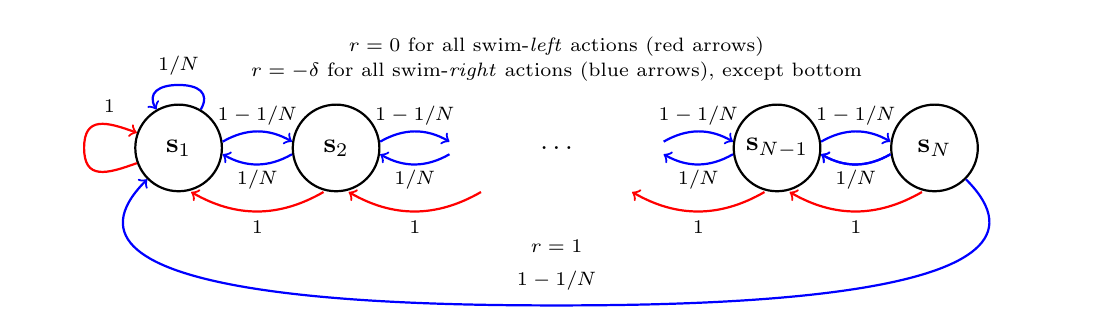
\begin{tikzpicture}[scale=0.8]
\node[draw,thick,circle,minimum size=1.1cm,inner sep=0pt, fill=white] (a) at (0,0) {$\s_1$};
\node[draw,thick,circle,minimum size=1.1cm,inner sep=0pt, fill=white] (b) at (2.5,0) {$\s_2$};
\node (c) at (5,0) {};
\node (d) at (7,0) {};
\node[draw,thick,circle,minimum size=1.1cm,inner sep=0pt, fill=white] (e) at (9.5,0) {$\s_{N-1}$};
\node[draw,thick,circle,minimum size=1.1cm,inner sep=0pt, fill=white] (f) at (12,0) {$\s_N$};

\draw[bend left,->,thick, blue]  ($(a) + (0.7, 0.1)$) to node [auto] {} ($(b) - (0.7, -0.1)$);
\draw[bend left,->,thick, blue]  ($(b) - (0.7, 0.1)$) to node [auto] {} ($(a) + (0.7, -0.1)$);
\draw[bend left,->,thick, red]  ($(b) - (0.2, 0.7)$) to node [auto] {} ($(a) + (0.2, -0.7)$);
\node[anchor=south] at ($(a) + (1.25, 0.2)$) {\scriptsize{$1 - 1/N$}};
\node[anchor=north] at ($(a) + (1.25, -0.2)$) {\scriptsize{$1/N$}};
\node[anchor=north] at ($(a) + (1.25, -1.0)$) {\scriptsize{$1$}};

\draw[bend left,->,thick, blue]  ($(b) + (0.7, 0.1)$) to node [auto] {} ($(c) - (0.7, -0.1)$);
\draw[bend left,->,thick, blue]  ($(c) - (0.7, 0.1)$) to node [auto] {} ($(b) + (0.7, -0.1)$);
\draw[bend left,->,thick, red]  ($(c) - (0.2, 0.7)$) to node [auto] {} ($(b) + (0.2, -0.7)$);
\node[anchor=south] at ($(b) + (1.25, 0.2)$) {\scriptsize{$1 - 1/N$}};
\node[anchor=north] at ($(b) + (1.25, -0.2)$) {\scriptsize{$1/N$}};
\node[anchor=north] at ($(b) + (1.25, -1.0)$) {\scriptsize{$1$}};

\draw[bend left,->,thick, blue]  ($(d) + (0.7, 0.1)$) to node [auto] {} ($(e) - (0.7, -0.1)$);
\draw[bend left,->,thick, blue]  ($(e) - (0.7, 0.1)$) to node [auto] {} ($(d) + (0.7, -0.1)$);
\draw[bend left,->,thick, red]  ($(e) - (0.2, 0.7)$) to node [auto] {} ($(d) + (0.2, -0.7)$);
\node[anchor=south] at ($(d) + (1.25, 0.2)$) {\scriptsize{$1 - 1/N$}};
\node[anchor=north] at ($(d) + (1.25, -0.2)$) {\scriptsize{$1/N$}};
\node[anchor=north] at ($(d) + (1.25, -1.0)$) {\scriptsize{$1$}};

\draw[bend left,->,thick, blue]  ($(e) + (0.7, 0.1)$) to node [auto] {} ($(f) - (0.7, -0.1)$);
\draw[bend left,->,thick, blue]  ($(f) - (0.7, 0.1)$) to node [auto] {} ($(e) + (0.7, -0.1)$);
\draw[bend left,->,thick, red]  ($(f) - (0.2, 0.7)$) to node [auto] {} ($(e) + (0.2, -0.7)$);
\node[anchor=south] at ($(e) + (1.25, 0.2)$) {\scriptsize{$1 - 1/N$}};
\node[anchor=north] at ($(e) + (1.25, -0.2)$) {\scriptsize{$1/N$}};
\node[anchor=north] at ($(e) + (1.25, -1.0)$) {\scriptsize{$1$}};

\draw [->, thick, red] (a) to[out=-160, in=-90,looseness=1.5] ($(a) - (1.5, 0)$)    to[out=90,in=160,looseness=1.5] (a);
\draw [->, thick, blue] (a) to[out=60, in=0,looseness=1.5] ($(a) + (0, 1)$)    to[out=180,in=120,looseness=1.5] (a);
\draw [->, thick, blue] (f) to[out=-45, in=0,looseness=1] (6, -2.5)    to[out=180,in=-135,looseness=1] (a);
\node[anchor=south] at ($(a) + (-1.10, 0.40)$) {\scriptsize{$1$}};
\node[anchor=south] at ($(a) + (0.00, 1.00)$) {\scriptsize{$1/N$}};
\node[anchor=south] at (6, 1.3) {\scriptsize{$r = 0$} \text{for all swim-\textit{left} actions (red arrows)}};
\node[anchor=south] at (6, 0.9) {\scriptsize{$r = -\delta$} \text{for all swim-\textit{right} actions (blue arrows), except bottom}};
\node[anchor=south] at (6, -2.5) {\begin{tabular}{c} \scriptsize{$r = 1$} \\  \scriptsize{$1 - 1/N$} \end{tabular}};

\draw[bend left,->,thick, blue]  ($(f) - (0.7, 0.1)$) to node [auto] {} ($(e) + (0.7, -0.1)$);

\node (e) at (6,0) {$\hdots$};
\end{tikzpicture}
\caption[DeepSea MDP]{DeepSea MDP from the continuing setting, modified from \cite{deepsea}. Blue arrows correspond to swim-\textit{right} (optimal) and red arrows to swim-\textit{left} (sub-optimal).}\label{deepseaMDP}
\end{figure}
This environment is designed to test whether the agent continues exploring despite receiving negative rewards. Sustained exploration becomes increasingly important for large $N$. As argued in \cite{iothesis}, in order to avoid exponentially poor performance, exploration in such chain-like environments must be guided by uncertainty rather than randomness.

\subsection{WideNarrow}

The WideNarrow MDP (\cref{widenarrowMDP}) has $2N + 1$ states and deterministic transitions. Odd states except $\s_{2N + 1}$ have $W$ actions, out of which one gives $r \sim \mc{N}(\mu_h, \sigma^2)$ whereas all others give $r \sim \mc{N}(\mu_l, \sigma^2)$, with $\mu_l < \mu_h$. Even states have a single action also giving $r \sim \mc{N}(\mu_l, \sigma^2)$. In our experiments we use $\mu_h = 0.5, \mu_l = 0$ and $\sigma_h = \sigma_l = 1$.

\begin{figure}[h!]
\centering
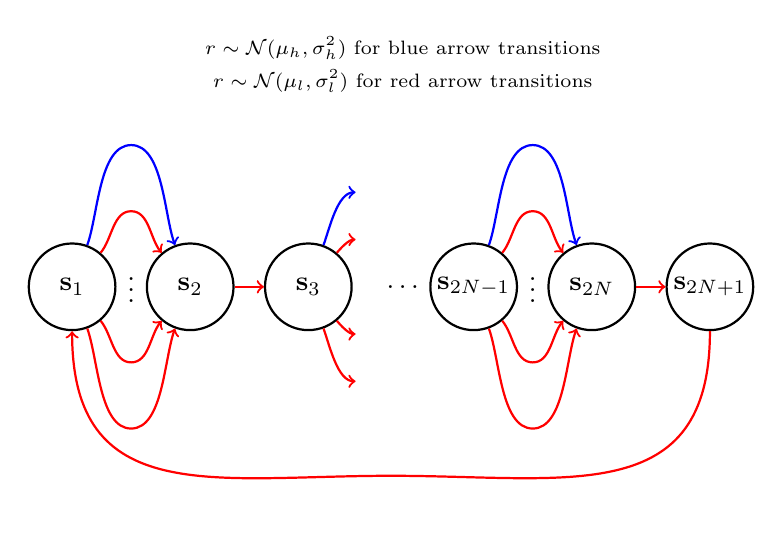
\begin{tikzpicture}[scale=0.6]
\node[draw,thick,circle,minimum size=1.1cm,inner sep=0pt, fill=white] (a) at (0,0) {$\s_1$};
\node[draw,thick,circle,minimum size=1.1cm,inner sep=0pt, fill=white] (b) at (2.5,0) {$\s_2$};
\node[draw,thick,circle,minimum size=1.1cm,inner sep=0pt, fill=white] (c) at (5,0) {$\s_3$};

\node (z) at (1.25,0.1) {$\vdots$};

\draw [->, thick, blue] (a) to[out=70, in=-180,looseness=0.75] (1.25, 3) to[out=0,in=110,looseness=0.75] (b);
\draw [->, thick, red] (a) to[out=50, in=-180,looseness=0.9] (1.25, 1.6) to[out=0,in=130,looseness=0.9] (b);
\draw [->, thick, red] (a) to[out=-50, in=-180,looseness=0.9] (1.25, -1.6) to[out=0,in=-130,looseness=0.9] (b);
\draw [->, thick, red] (a) to[out=-70, in=-180,looseness=0.75] (1.25, -3) to[out=0,in=-110,looseness=0.75] (b);

\draw [->, thick, red] (b) to (c);

\draw [->, thick, blue] (c) to[out=70, in=-180,looseness=0.75] ($(c) + (1, 2)$);
\draw [->, thick, red] (c) to[out=50, in=-180,looseness=0.75] ($(c) + (1, 1)$);
\draw [->, thick, red] (c) to[out=-50, in=-180,looseness=0.75] ($(c) + (1, -1)$);
\draw [->, thick, red] (c) to[out=-70, in=-180,looseness=0.75] ($(c) + (1, -2)$);

\node (g) at (7.00, 0.0) {$\hdots$};

\node[draw,thick,circle,minimum size=1.1cm,inner sep=0pt, fill=white] (d) at (8.5,0) {$\s_{2N - 1}$};
\node[draw,thick,circle,minimum size=1.1cm,inner sep=0pt, fill=white] (e) at (11,0) {$\s_{2N}$};
\node[draw,thick,circle,minimum size=1.1cm,inner sep=0pt, fill=white] (f) at (13.5,0) {$\s_{2N + 1}$};

\draw [->, thick, blue] (d) to[out=70, in=-180,looseness=0.75] ($(d) + (1.25, 3)$) to[out=0,in=110,looseness=0.75] (e);
\draw [->, thick, red] (d) to[out=50, in=-180,looseness=0.9] ($(d) + (1.25, 1.6)$) to[out=0,in=130,looseness=0.9] (e);
\draw [->, thick, red] (d) to[out=-50, in=-180,looseness=0.9] ($(d) + (1.25, -1.6)$) to[out=0,in=-130,looseness=0.9] (e);
\draw [->, thick, red] (d) to[out=-70, in=-180,looseness=0.75] ($(d) + (1.25, -3)$) to[out=0,in=-110,looseness=0.75] (e);

\draw [->, thick, red] (e) to (f);
\node (g) at (9.75, 0.1) {$\vdots$};

\draw [->, thick, red] (f) to[out=-90, in=0,looseness=1.3] (6.75, -4) to[out=180,in=-90,looseness=1.3] (a);

\node[anchor=south] at (7, 4.6) {\scriptsize{$r \sim \mc{N}(\mu_h, \sigma^2_h)$} \text{for blue arrow transitions}};
\node[anchor=south] at (7, 3.9) {\scriptsize{$r \sim \mc{N}(\mu_l, \sigma^2_l)$} \text{for red arrow transitions}};
\end{tikzpicture}
\caption[WideNarrow MDP]{The WideNarrow MDP. All transitions are deterministic.}\label{widenarrowMDP}
\end{figure}

In general, the returns from different state-actions will be correlated under the posterior. Here, consider $(\s_1, \ac_1)$ and $(\s_1, \ac_2)$:
\begin{align}
\Cov_{z, \btheta} \sqb{ z^*_{\s_1, \ac_1}, z^*_{\s_1, \ac_2}} = &\Cov_{r, z, \btheta} \sqb{ r_{\s_1, \ac_1, \ns} + \gamma z^*_{\ns, \ac'}, ~r_{\s_1, \ac_2, \s{''}} + \gamma z^*_{\s{''}, \ac{''}}} \label{eq:cov_demo} \\
 =& \cancel{\Cov_{r, z, \btheta} \Big[ r_{\s_1, \ac_1, \ns}, r_{\s_1, \ac_2, \s{''}}\Big]} + \gamma \Cov_{r, \btheta} \sqb{r_{\s_1, \ac_1, \ns} , z^*_{\s{''}, \ac{''}} }\nonumber \\
&+ \gamma \Cov_{r, z, \btheta} \sqb{ r_{\s_1, \ac_2, \s{''}} , z^*_{\s{''}, \ac{''}} } + \gamma^2 \Cov_{z, \btheta} \sqb{z^*_{\ns, \ac'},  z^*_{\s{''}, \ac{''}}}\nonumber
\end{align}
where $\btheta$ loosely denotes all modelling parameters, $\s'$ denotes the next-state from $(\s_1, \ac_1)$, $\s{''}$ denotes the next-state from $(\s_1, \ac_2)$ and $\ac{'}, \ac{''}$ denote the corresponding next-actions. Although the remaining three terms are non-zero under the posterior, BQL, UBE and MM ignore them, instead sampling from a factored posterior. The WideNarrow environment enforces strong correlations between these state actions, allowing us to test the impact of a factored approximation.

\subsection{PriorMDP}

The aforementioned MDPs have very specific and handcrafted dynamics and rewards, so it is interesting to also compare the algorithms on environments which lack this sort of structure. For this we sample finite MDPs with $N_s$ states and $N_a$ actions from a prior distribution, as in \cite{psrl}. $\mct$ is a Categorical with parameters $\{\bs{\eta_{\s, \ac}}\}$ with:
\begin{align*}
\bs{\eta}_{\s, \ac} \sim \text{Dirichlet}(\bs{\kappa}_{\s, \ac}),
\end{align*}
with pseudo-count parameters $\bs{\kappa}_{\s, \ac} = \bm{1}$, while $\mcr \sim \mc{N}(\mu_{\s, \ac}, \tau_{\s, \ac}^{-1})$ with:
\begin{align*}
\mu_{\s, \ac}, \tau_{\s, \ac} \sim NG(\mu_{\s, \ac}, \tau_{\s, \ac} | \mu, \lambda, \alpha, \beta) \text{ with } (\mu, \lambda, \alpha, \beta) = (0.00, 1.00, 4.00, 4.00).
\end{align*}
We chose these hyperparameters because they give $Q^*$-values in a reasonable range.

\clearpage
\section{Supplementary figures} \label{app:supfig}

\subsection{DeepSea}

\begin{figure}[h!]
\centering
\begin{subfigure}{0.65\textwidth}
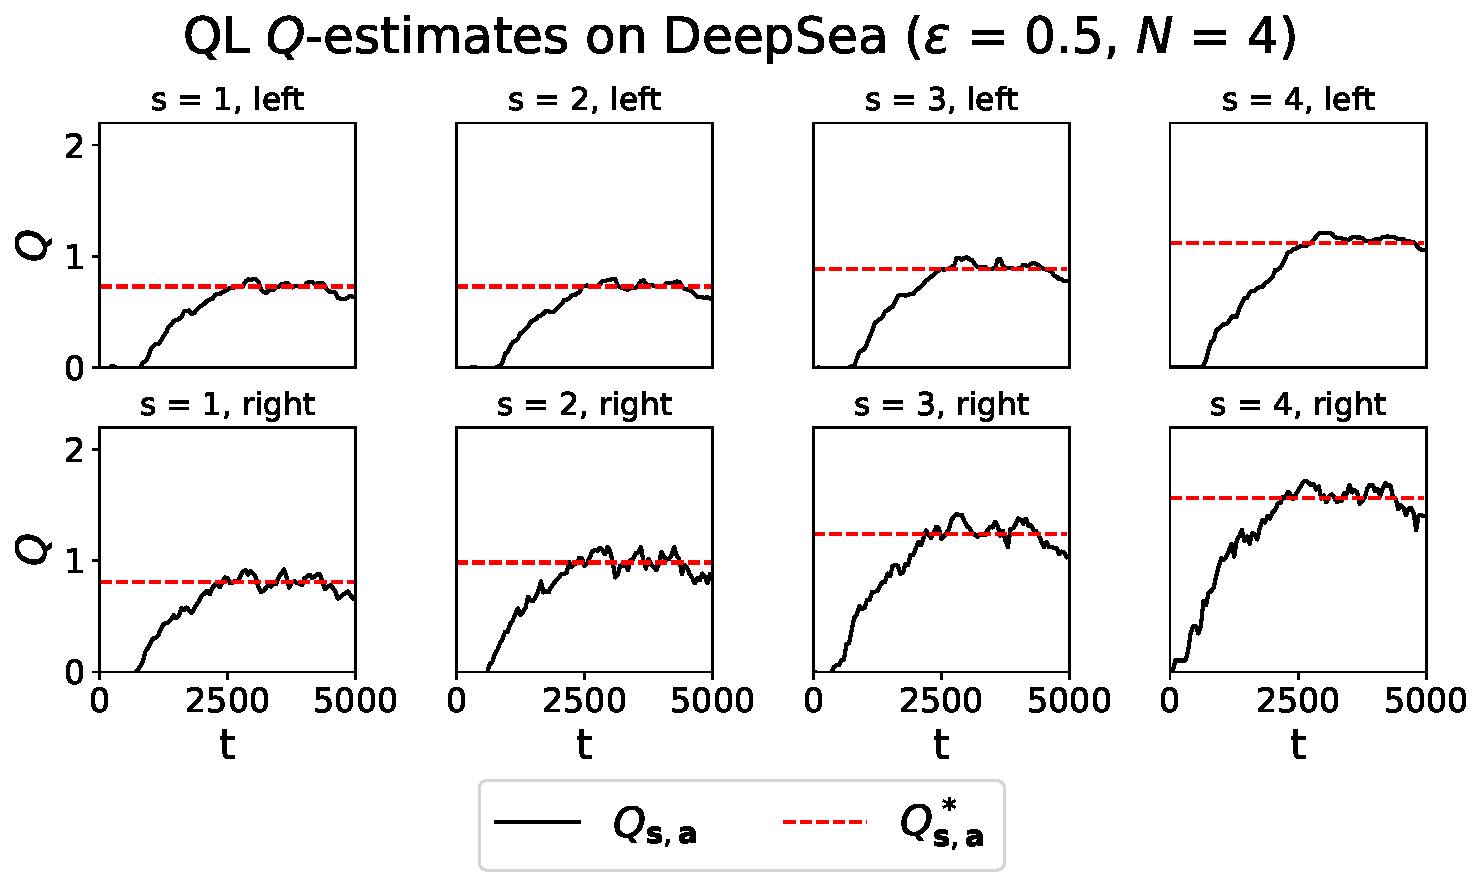
\includegraphics[width=\linewidth]{img/ql-0_5-qestimates-deepsea-4.pdf}
\end{subfigure}
\begin{subfigure}{0.34\textwidth}
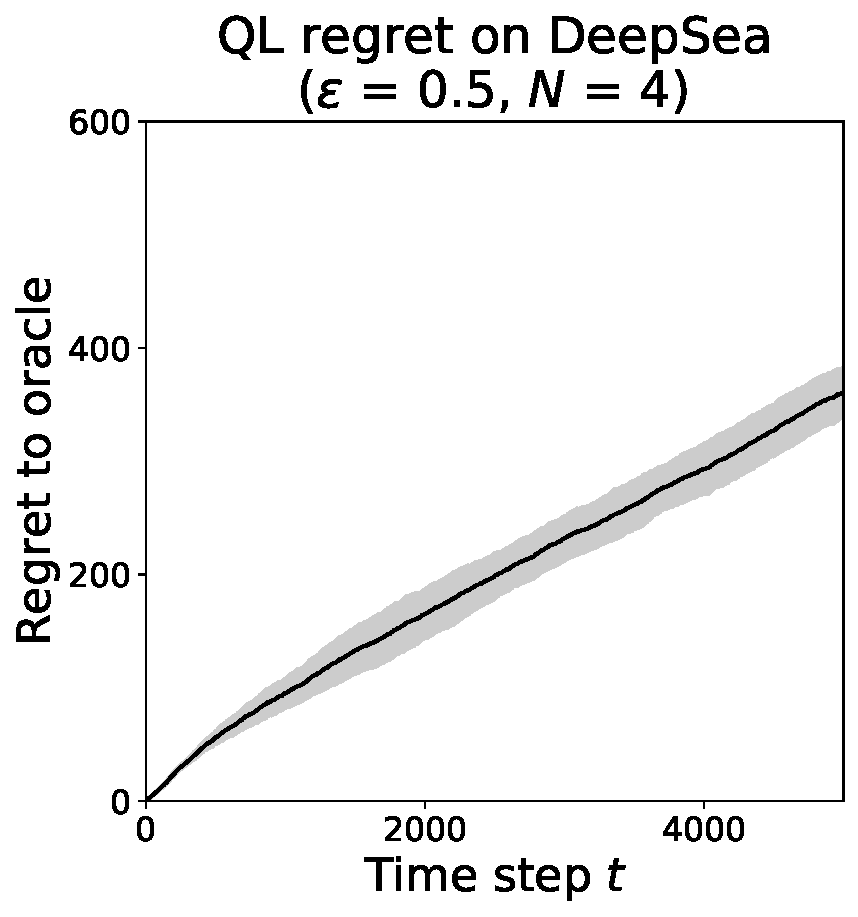
\includegraphics[width=\linewidth]{img/ql-0_5-regret-deepsea-4.pdf}~\\~\\
\end{subfigure}
\captionsetup{width=0.9\linewidth}
\caption{QL $Q$-estimates and regret on DeepSea.}\label{ql_deepsea_visual}
\end{figure}

\begin{figure}[h!]
\centering
\begin{subfigure}{0.65\textwidth}
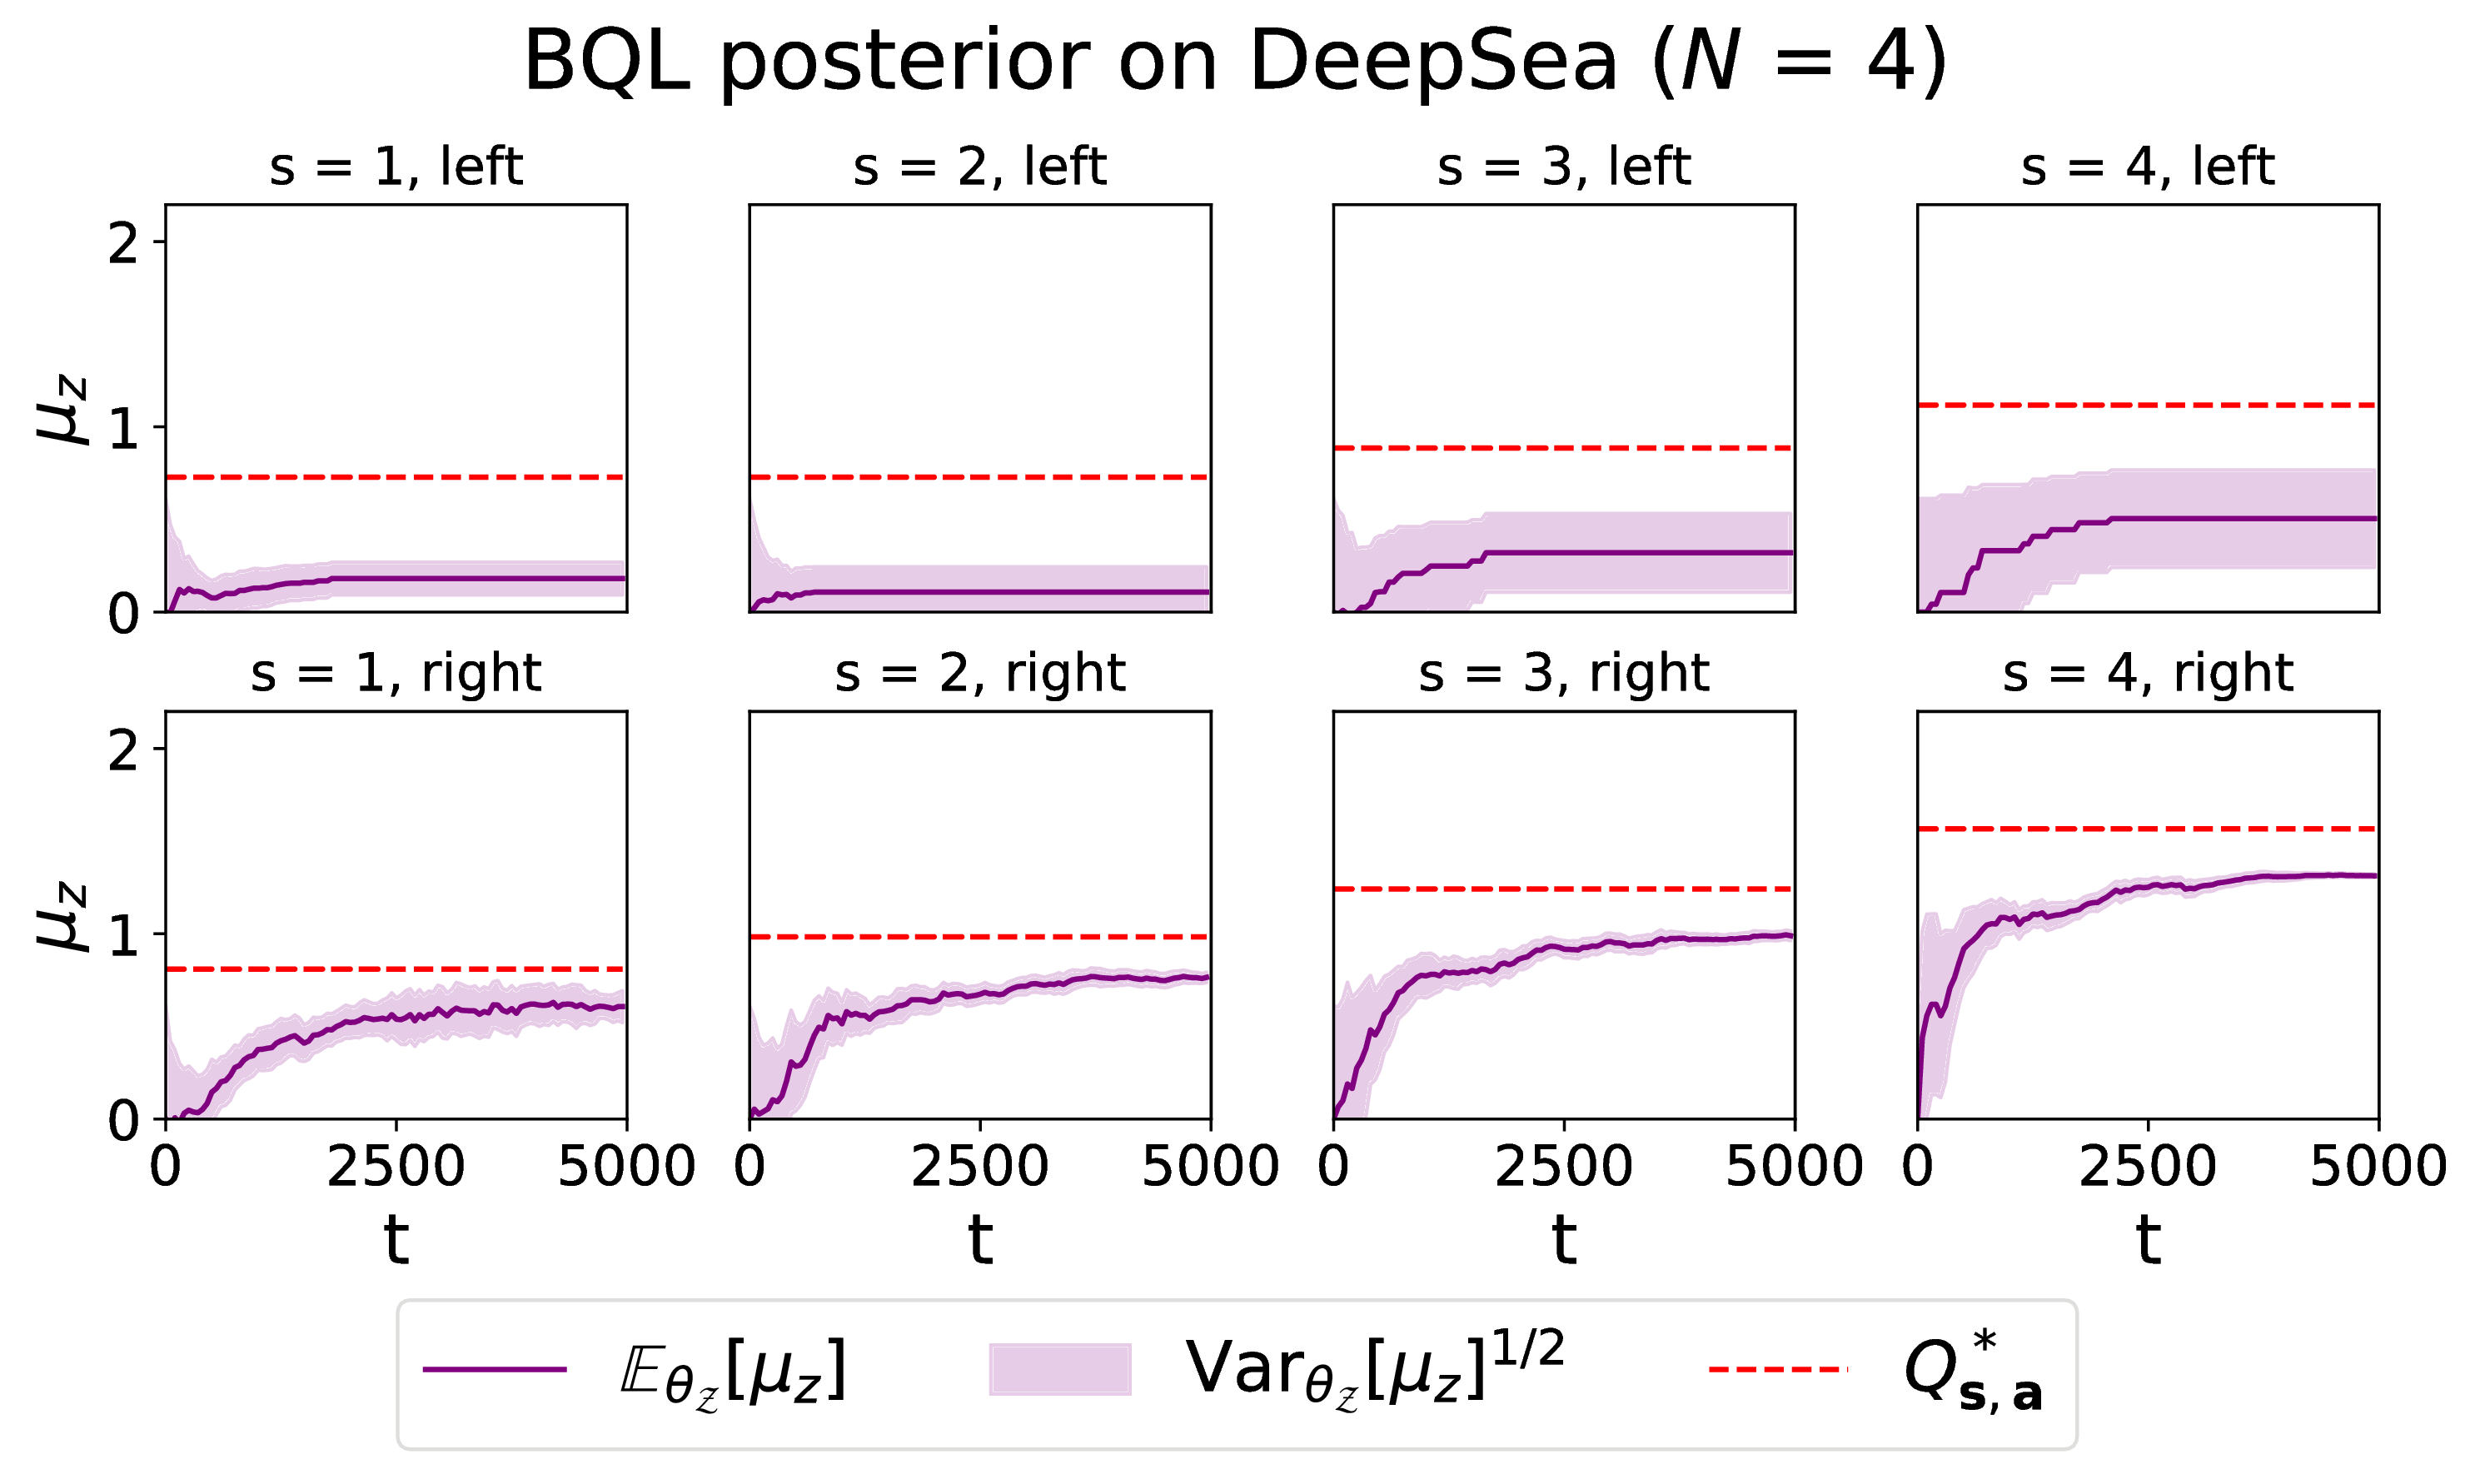
\includegraphics[width=\linewidth]{img/bql-0_0-4_0-3_0-3_0-posterior-deepsea-4.pdf}
\end{subfigure}
\begin{subfigure}{0.34\textwidth}
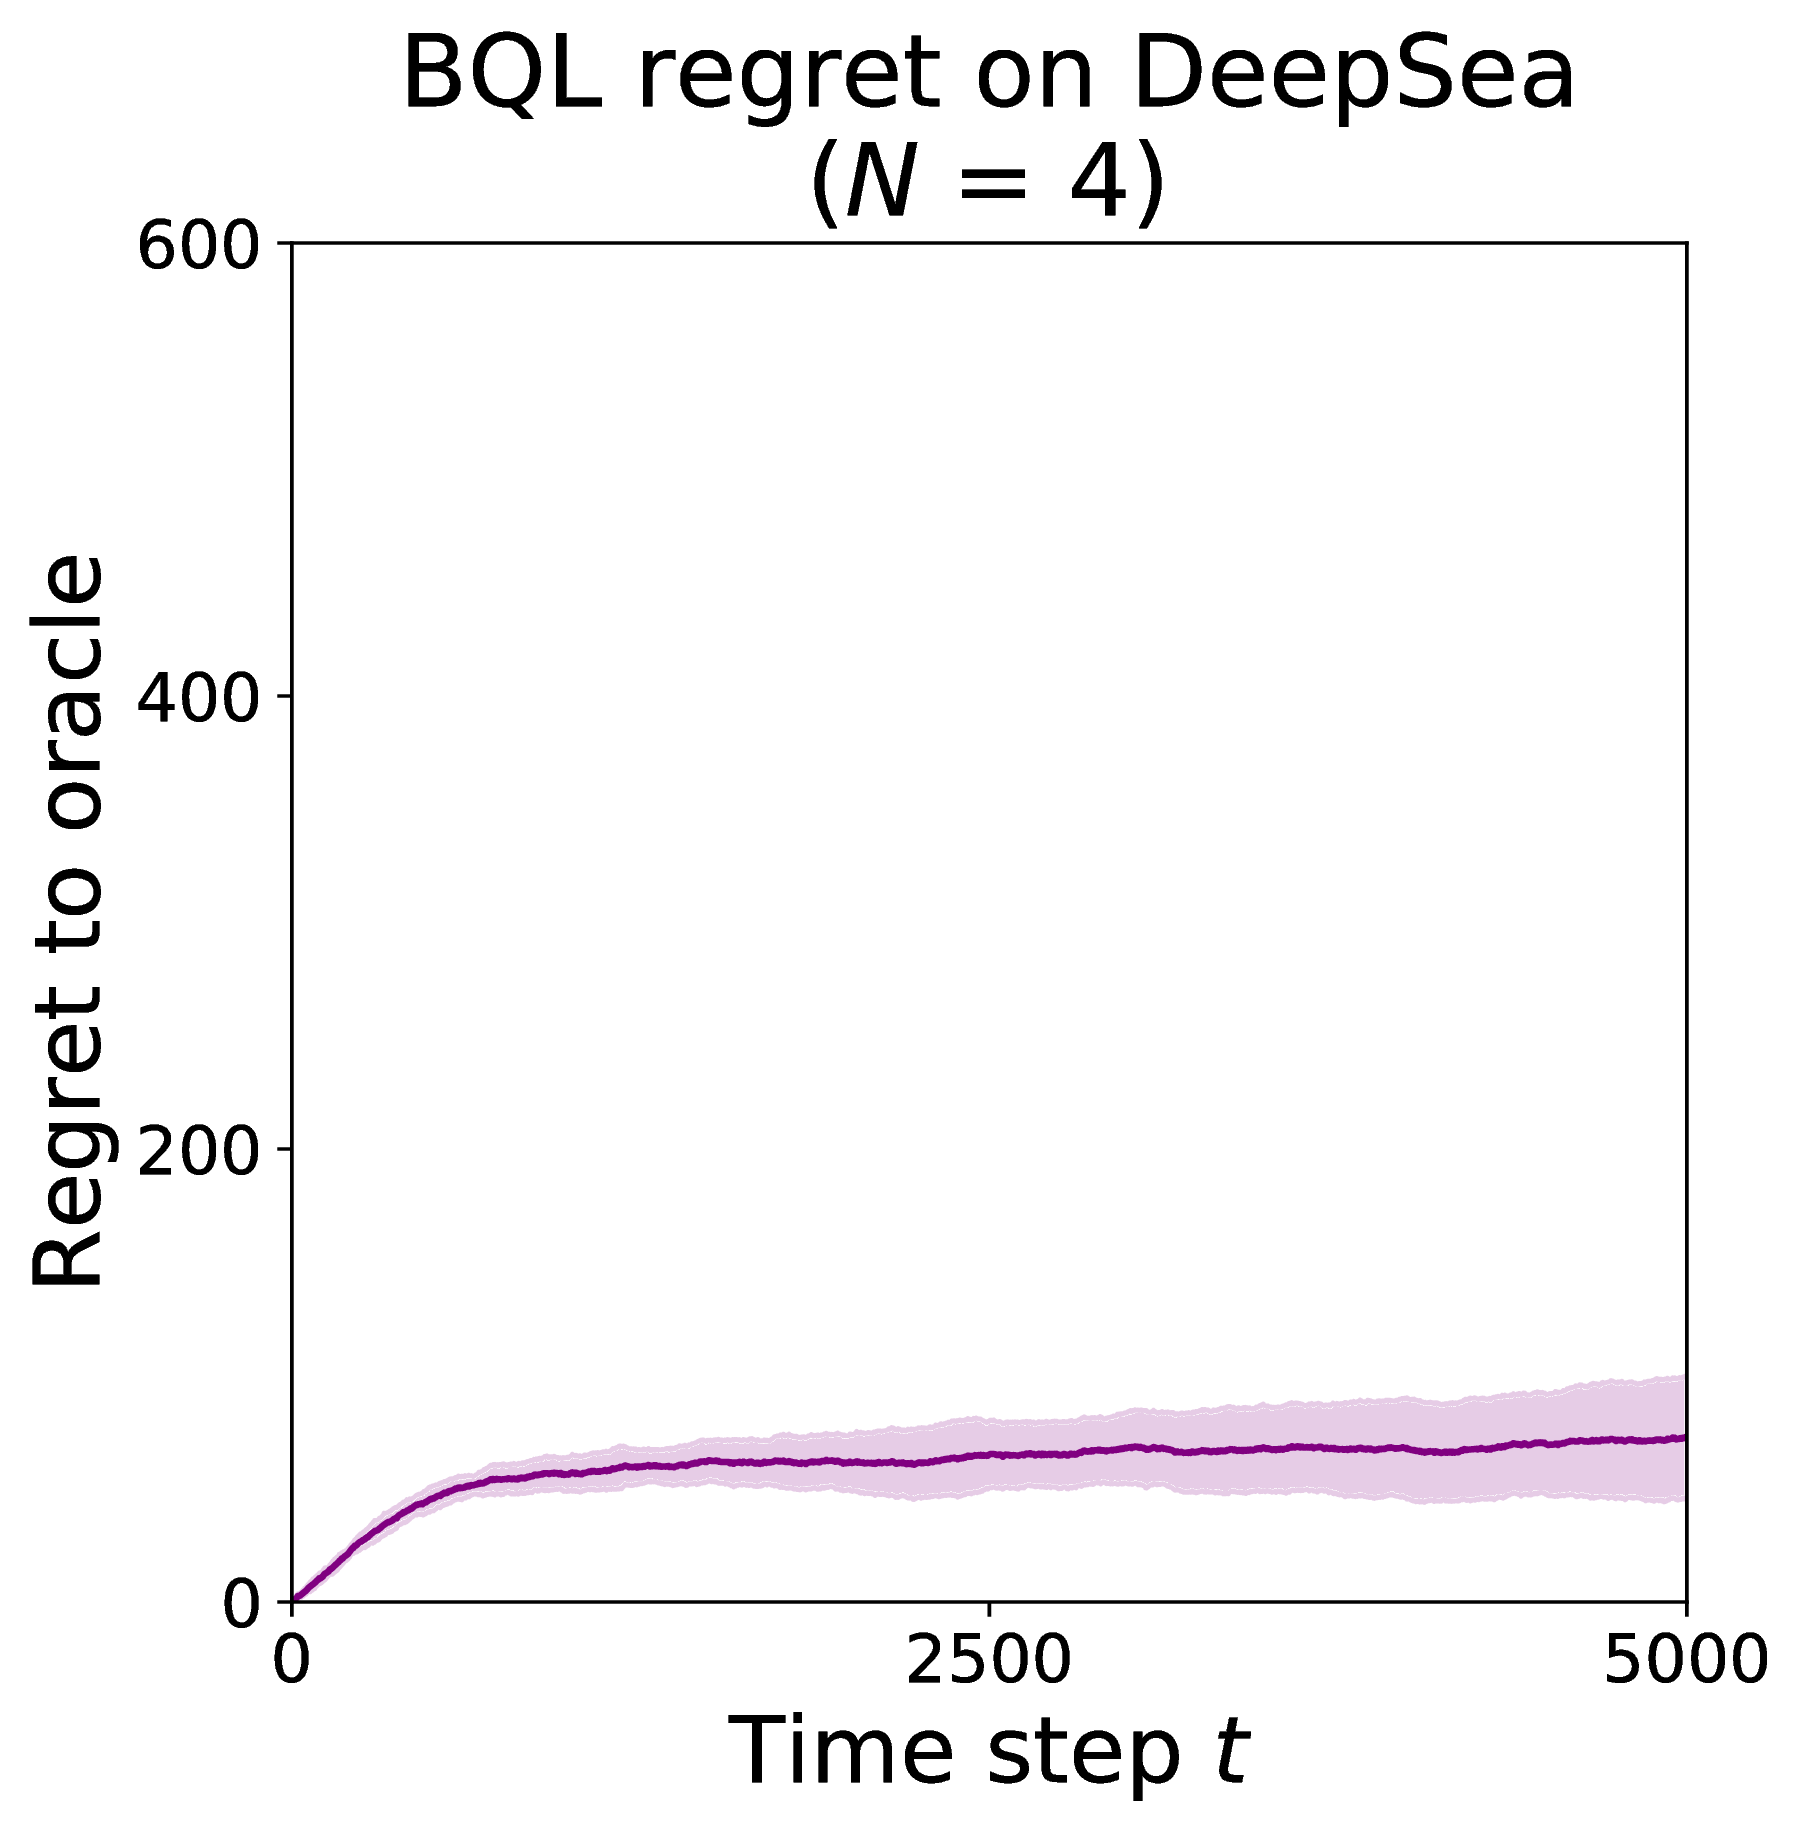
\includegraphics[width=\linewidth]{img/bql-0_0-4_0-3_0-3_0-regret-deepsea-4.pdf}~\\~\\
\end{subfigure}
\captionsetup{width=0.9\linewidth}
\caption{BQL posterior and regret on DeepSea.}\label{bql_deepsea_visual}
\end{figure}

\begin{figure}[h!]
\centering
\begin{subfigure}{0.65\textwidth}
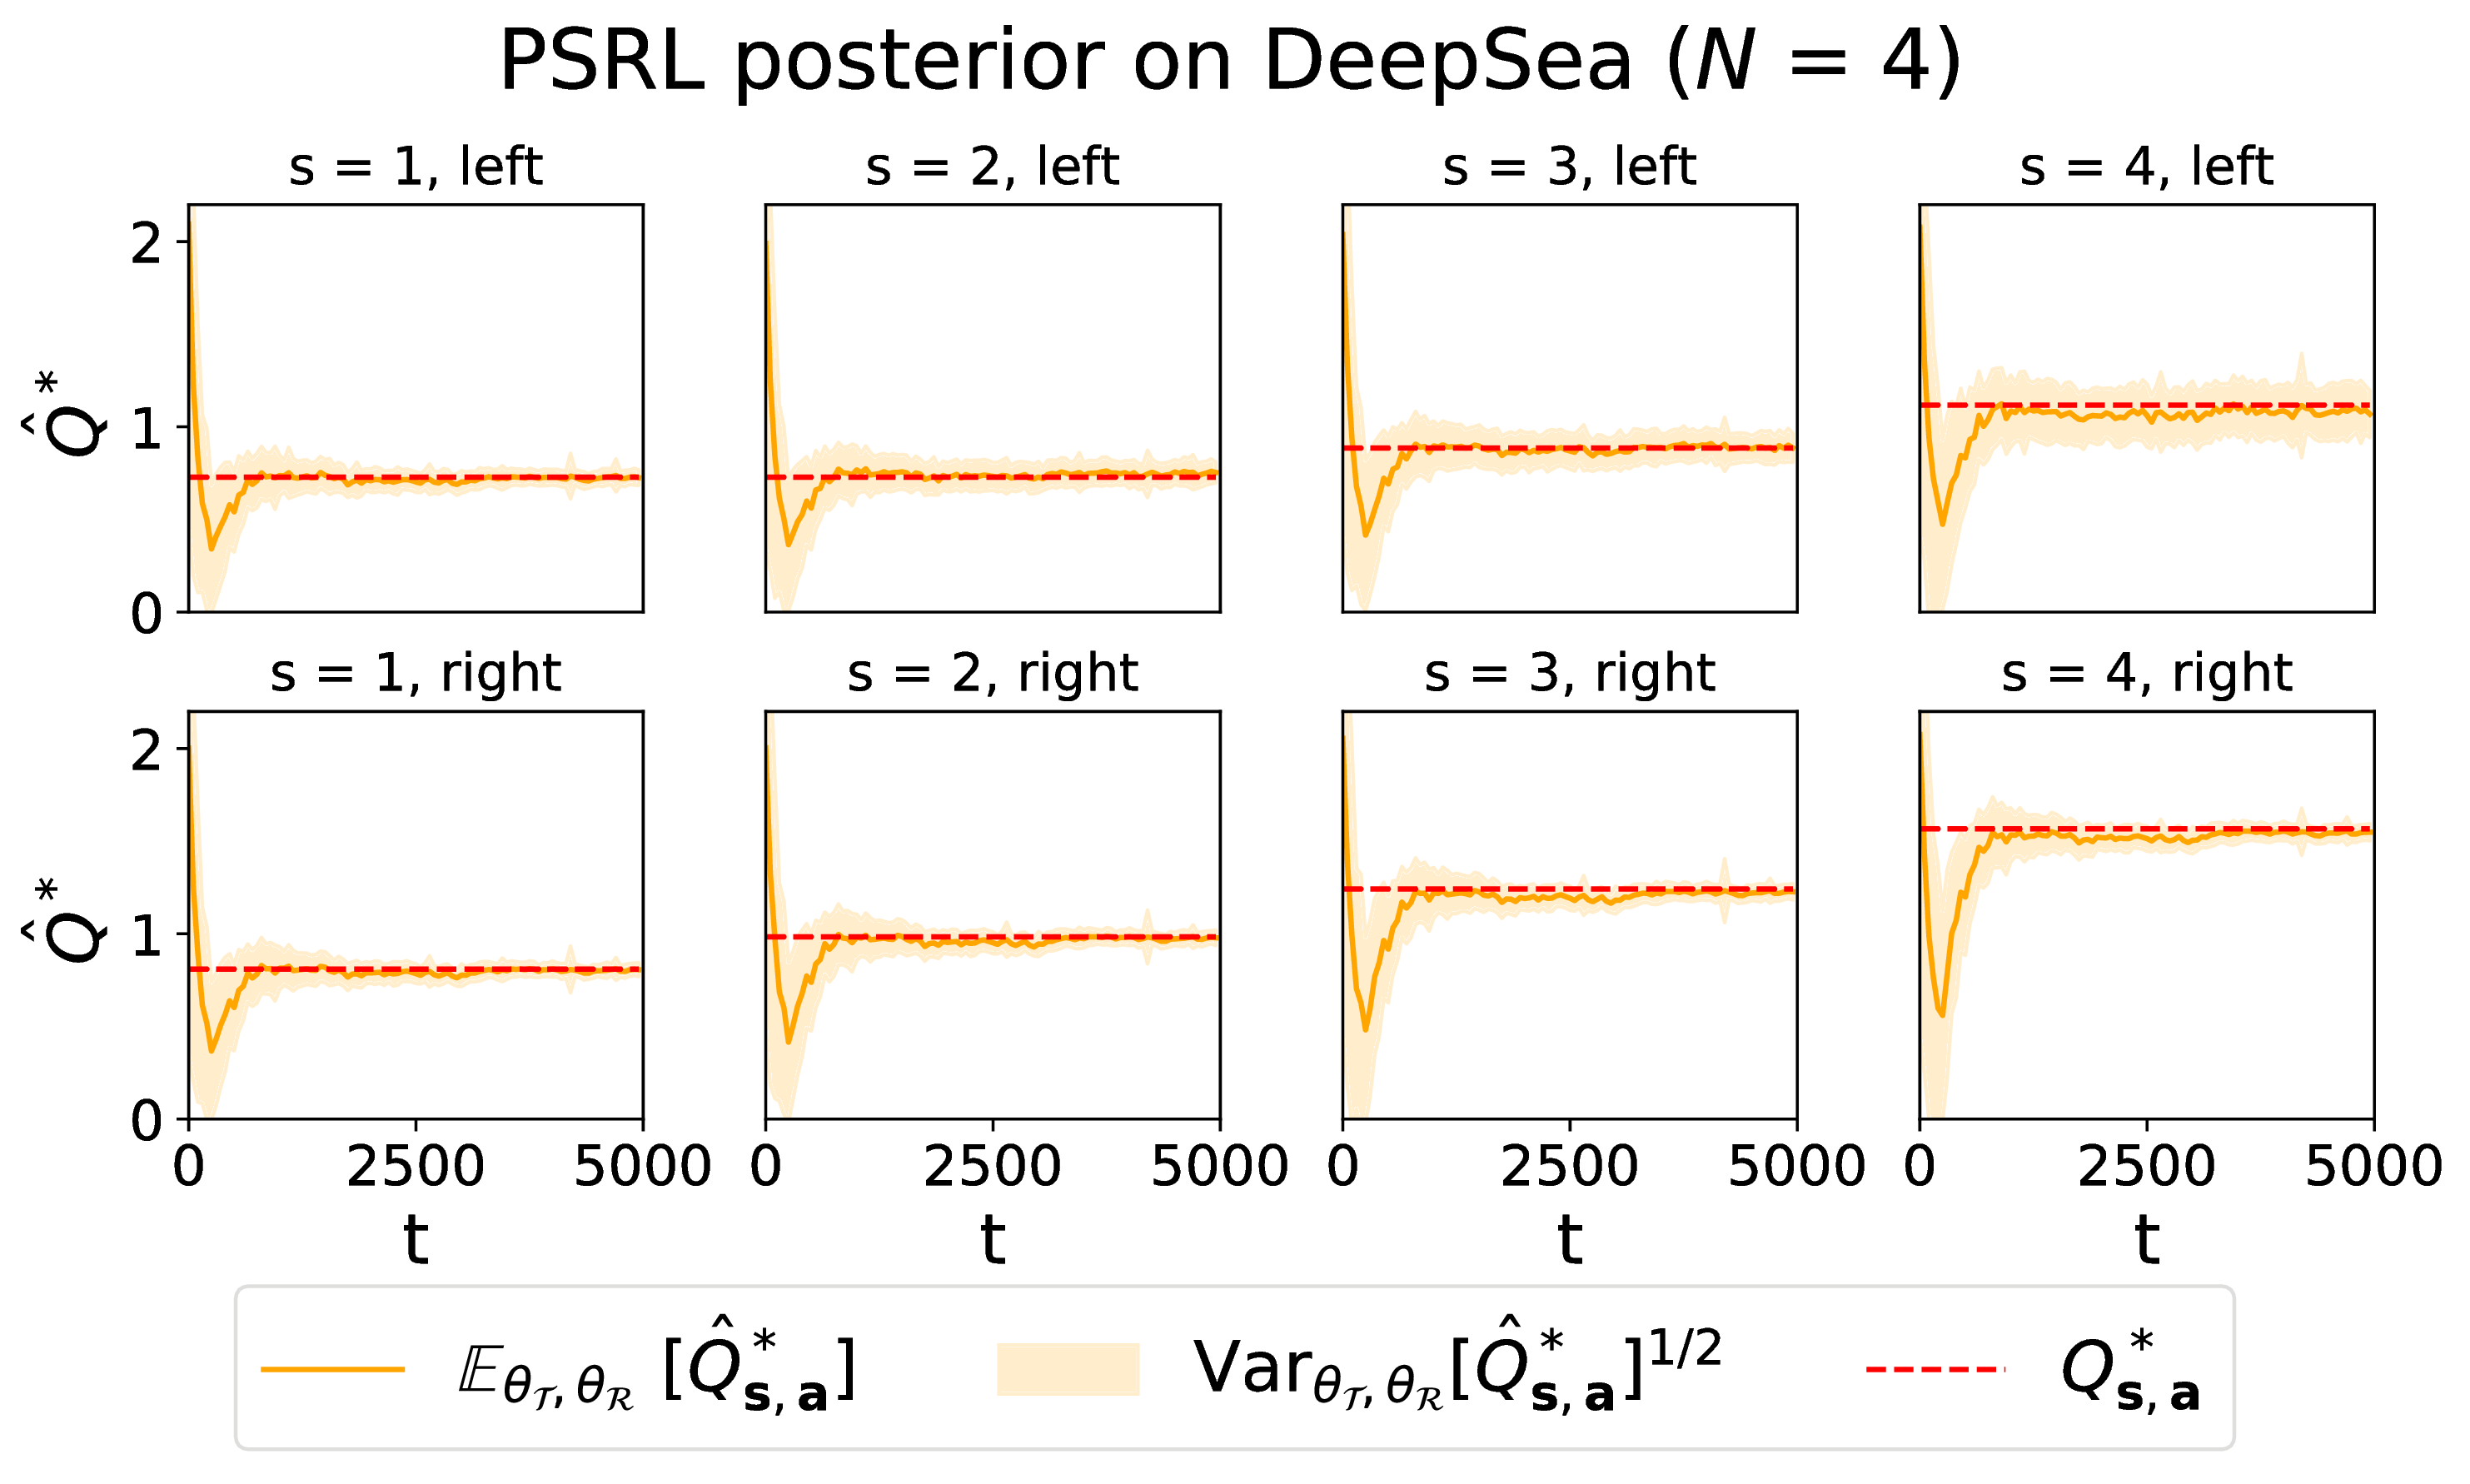
\includegraphics[width=\linewidth]{img/psrl-0_0-4_0-3_0-3_0-posterior-deepsea-4.pdf}
\end{subfigure}
\begin{subfigure}{0.34\textwidth}
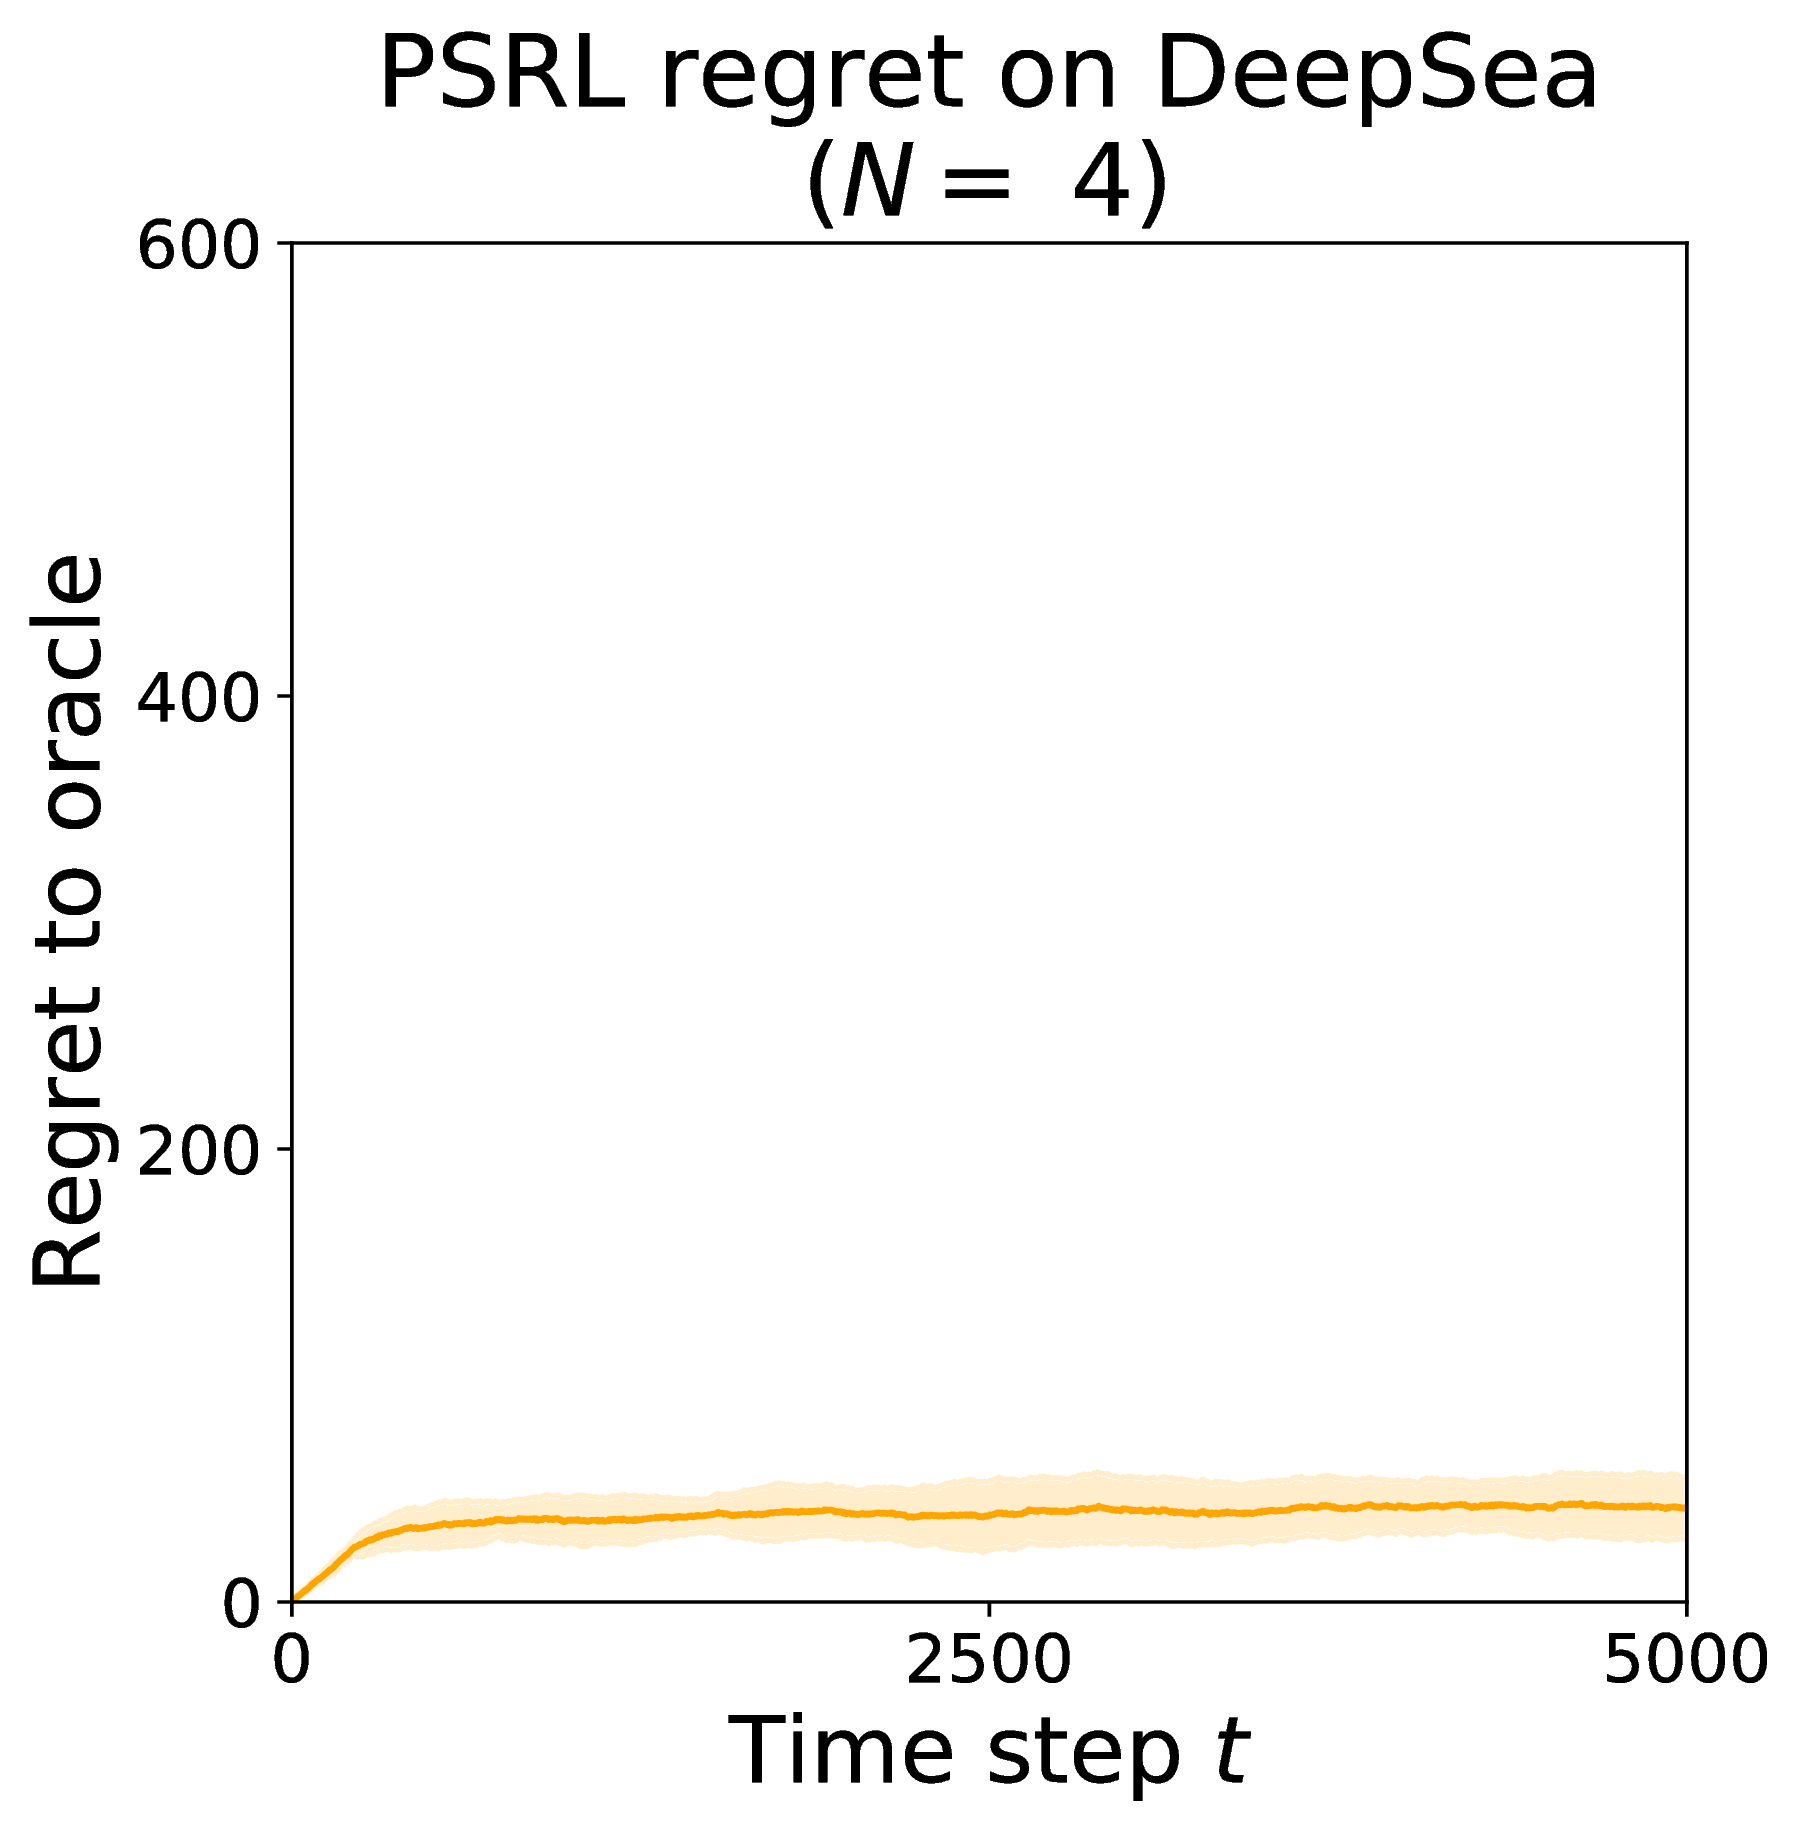
\includegraphics[width=\linewidth]{img/psrl-0_0-4_0-3_0-3_0-regret-deepsea-4.pdf}~\\~\\
\end{subfigure}
\captionsetup{width=0.9\linewidth}
\caption{PSRL posterior and regret on DeepSea.}\label{psrl_deepsea_visual}
\end{figure}

\begin{figure}[h!]
\centering
\begin{subfigure}{0.65\textwidth}
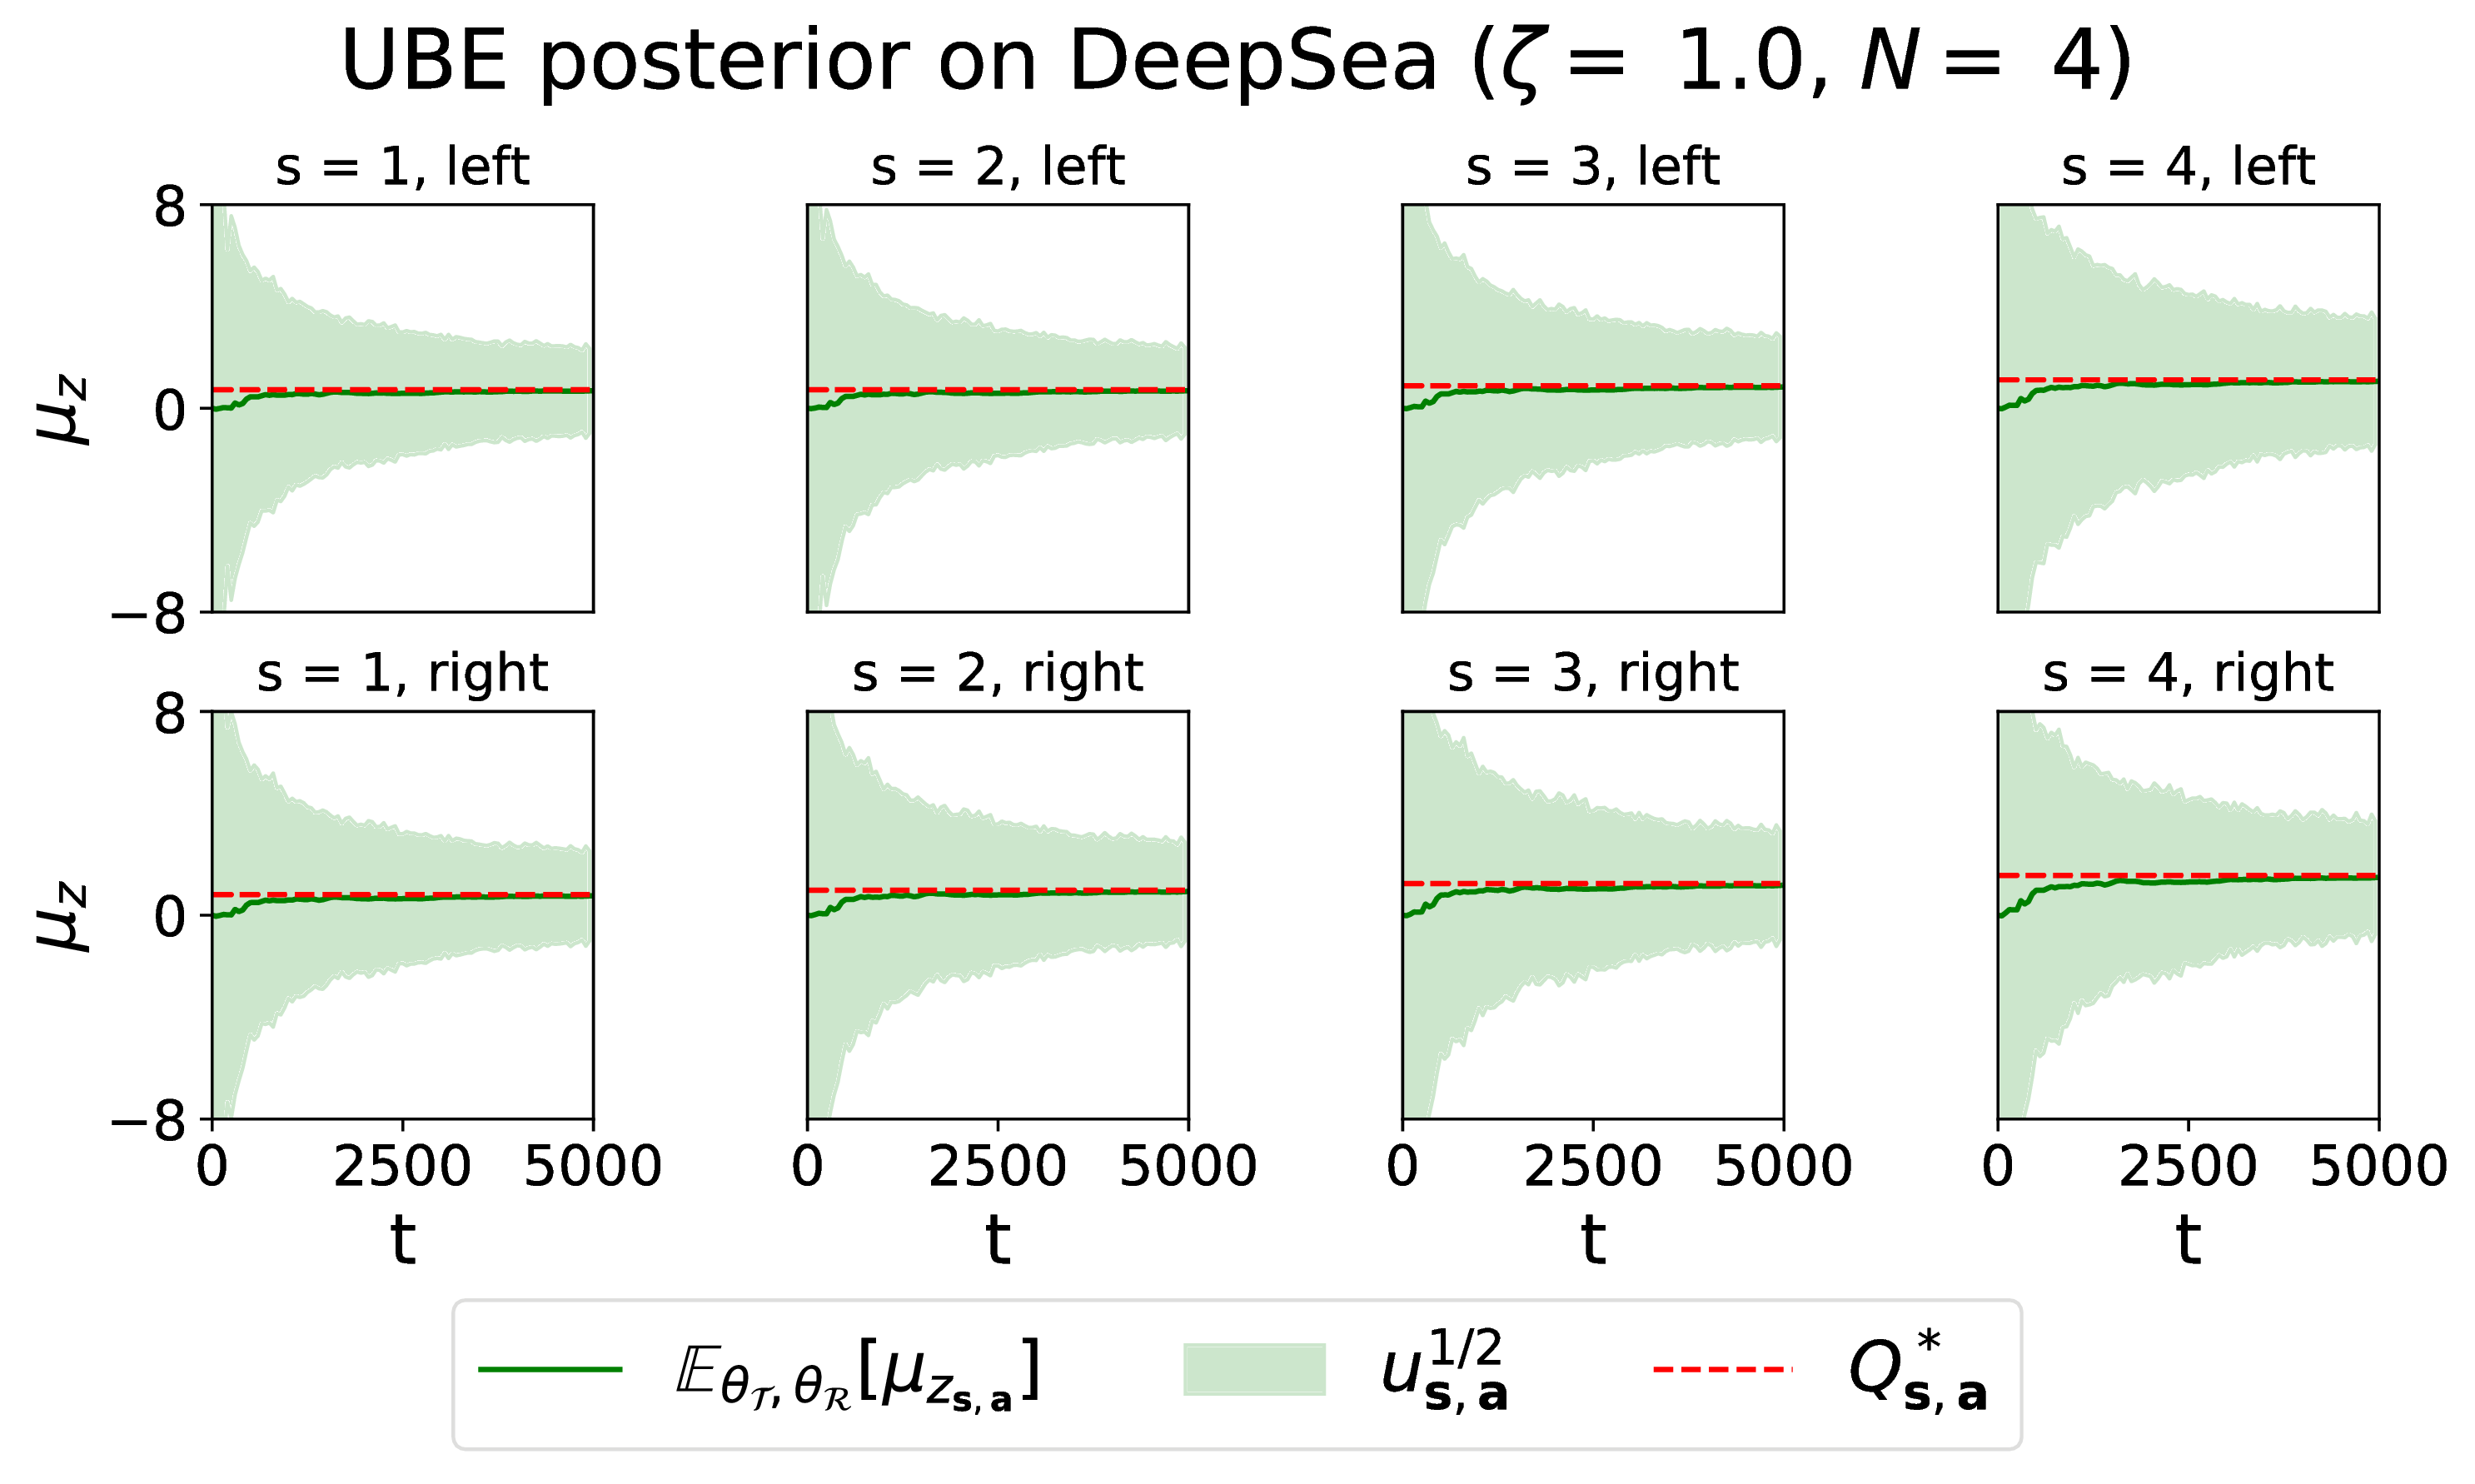
\includegraphics[width=\linewidth]{img/ube-0_0-4_0-3_0-3_0-1_0-posterior-deepsea-4.pdf}
\end{subfigure}
\begin{subfigure}{0.34\textwidth}
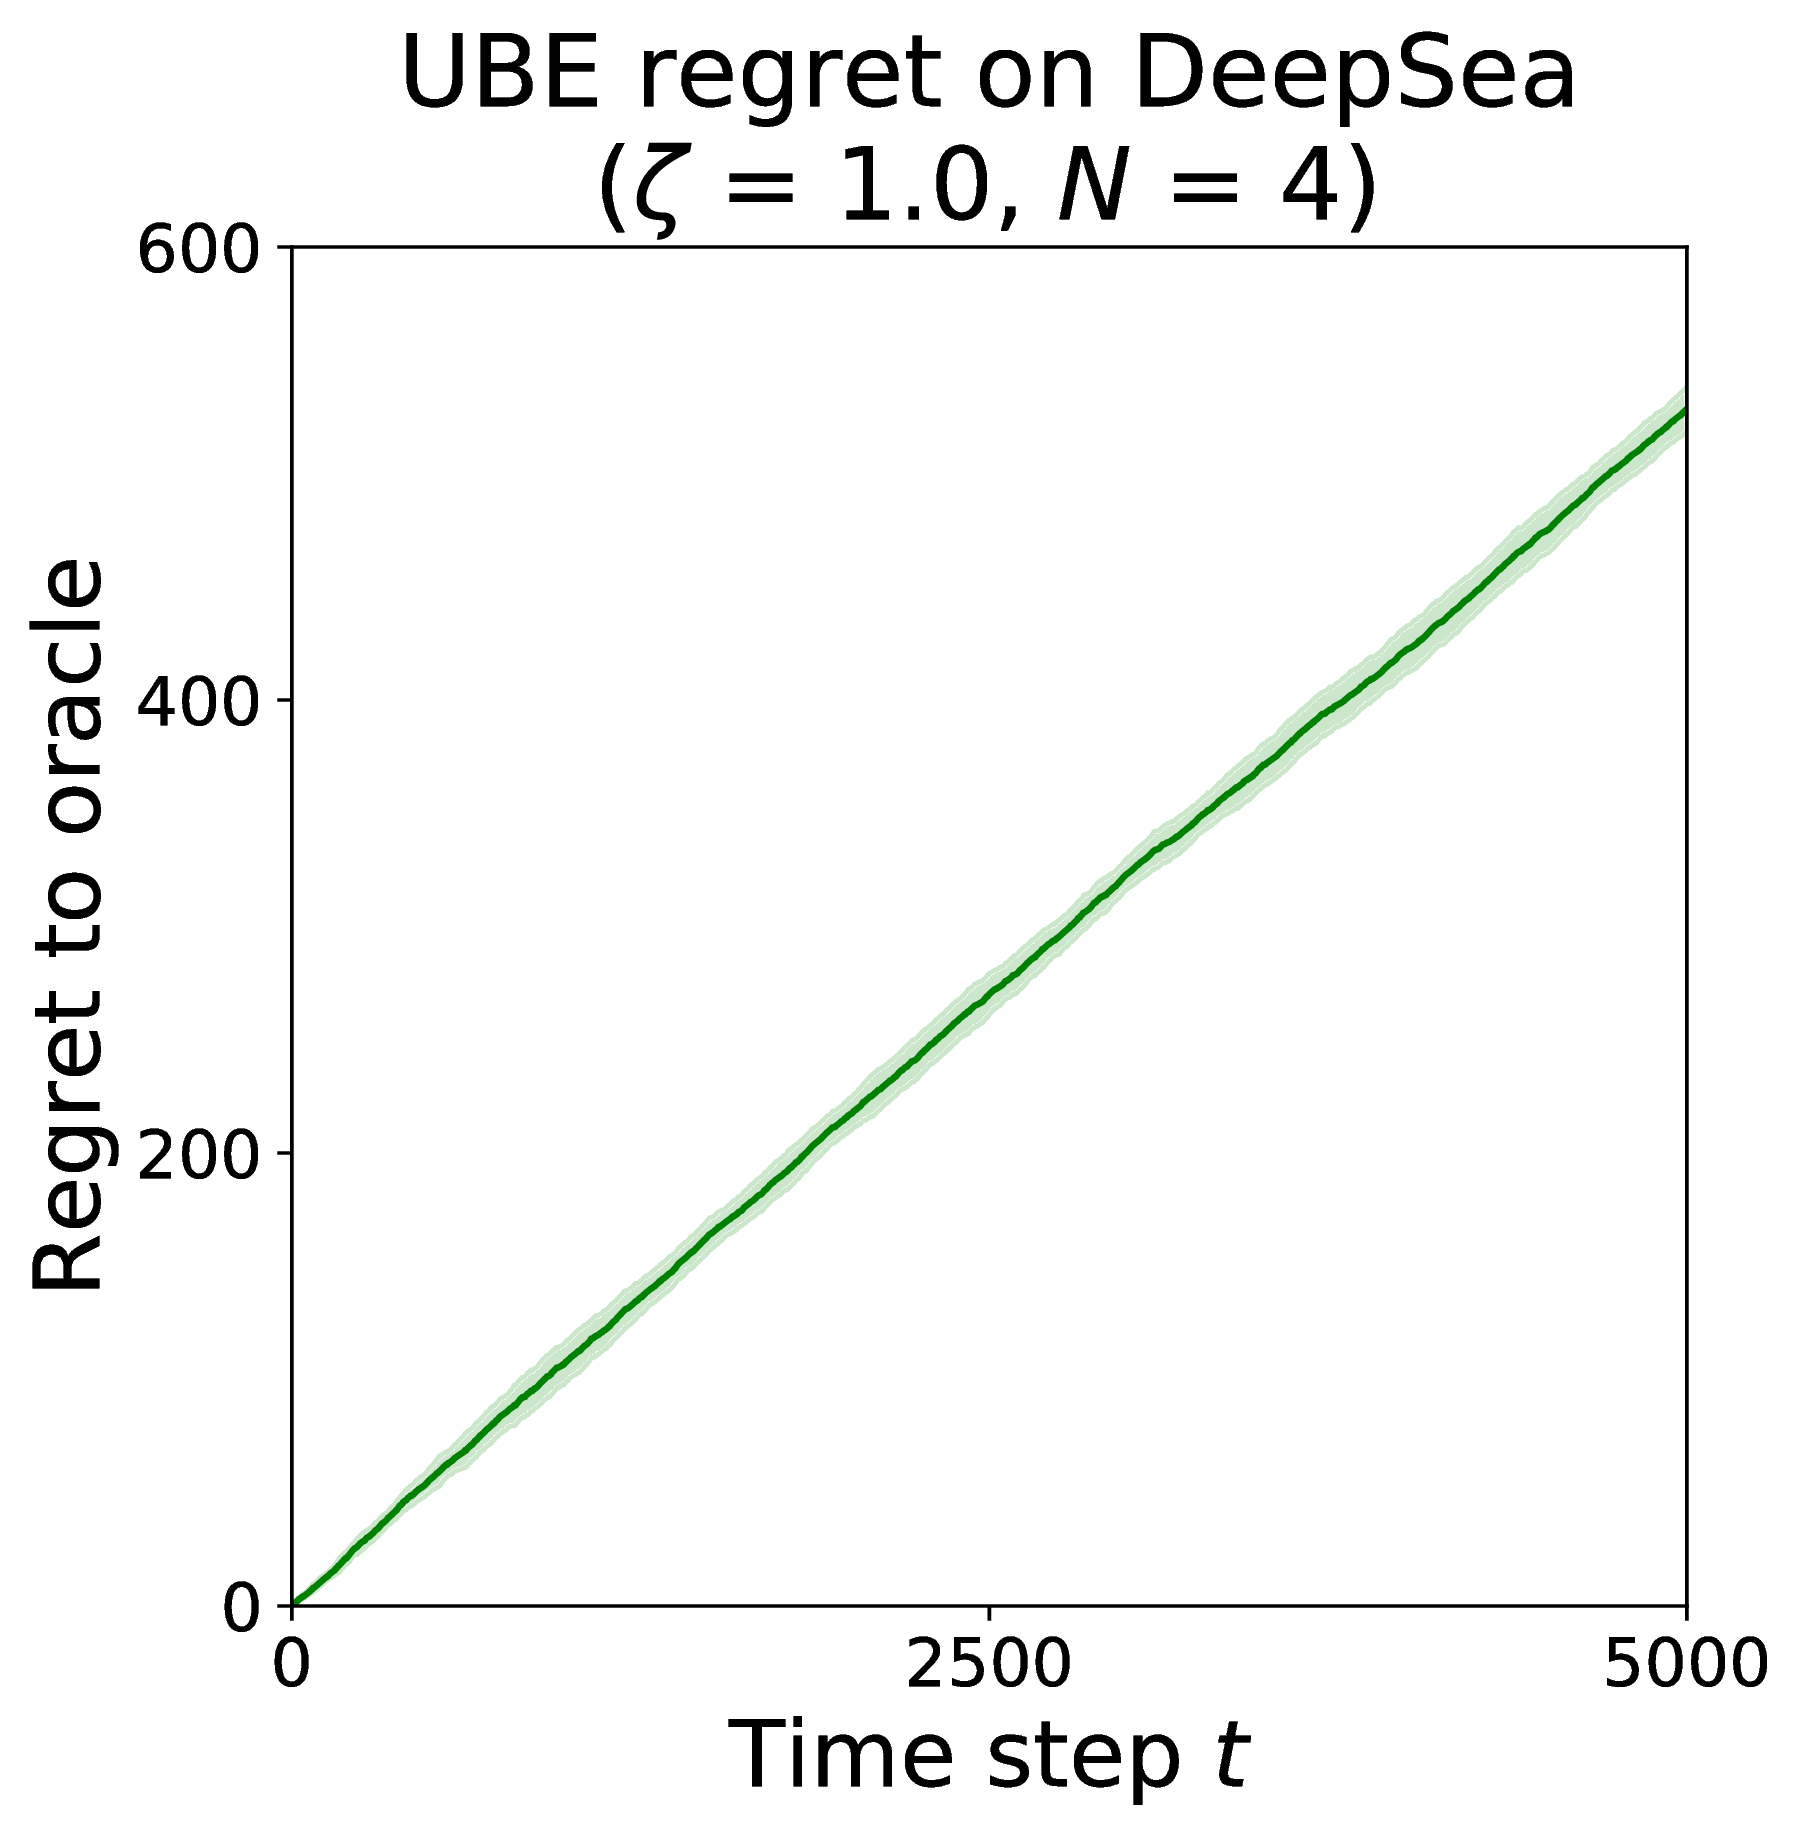
\includegraphics[width=\linewidth]{img/ube-0_0-4_0-3_0-3_0-1_0-regret-deepsea-4.pdf}~\\~\\
\end{subfigure}
\captionsetup{width=0.9\linewidth}
\caption{UBE posterior and regret on DeepSea.}\label{ube_deepsea_visual1}
\end{figure}

\begin{figure}[h!]
\centering
\vspace{-1cm}
\begin{subfigure}{0.65\textwidth}
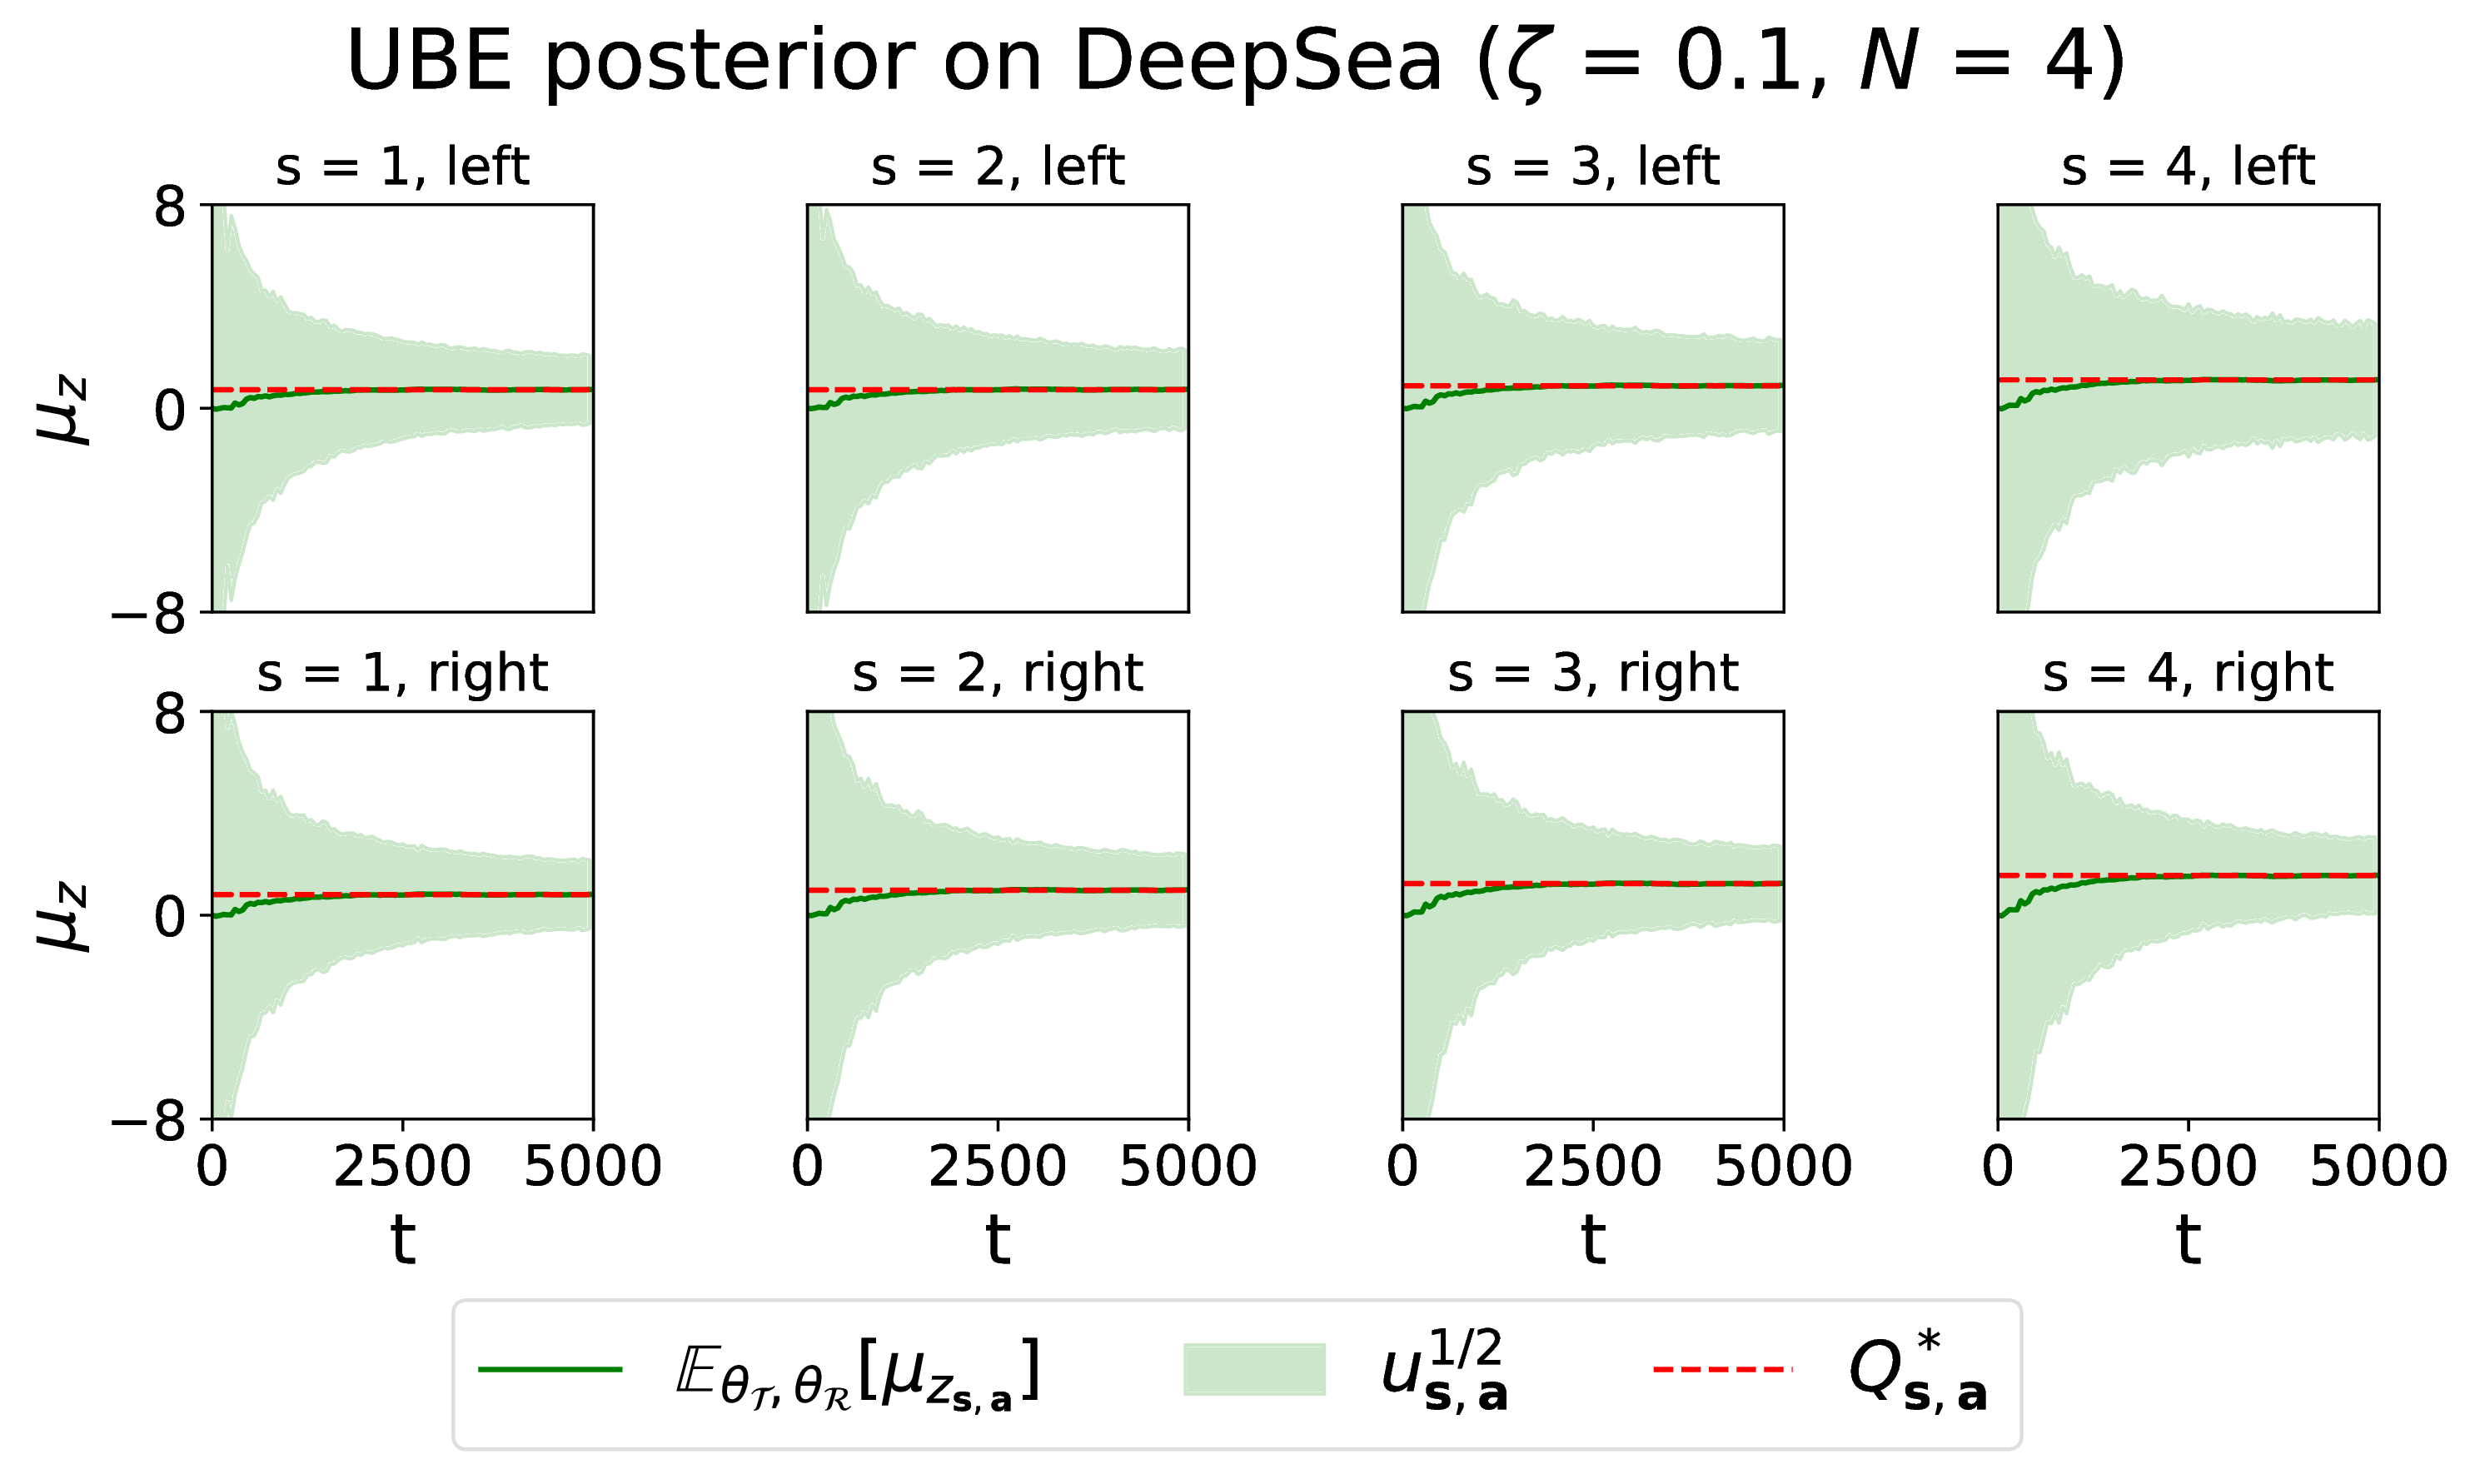
\includegraphics[width=\linewidth]{img/ube-0_0-4_0-3_0-3_0-0_1-posterior-deepsea-4.pdf}
\end{subfigure}
\begin{subfigure}{0.34\textwidth}
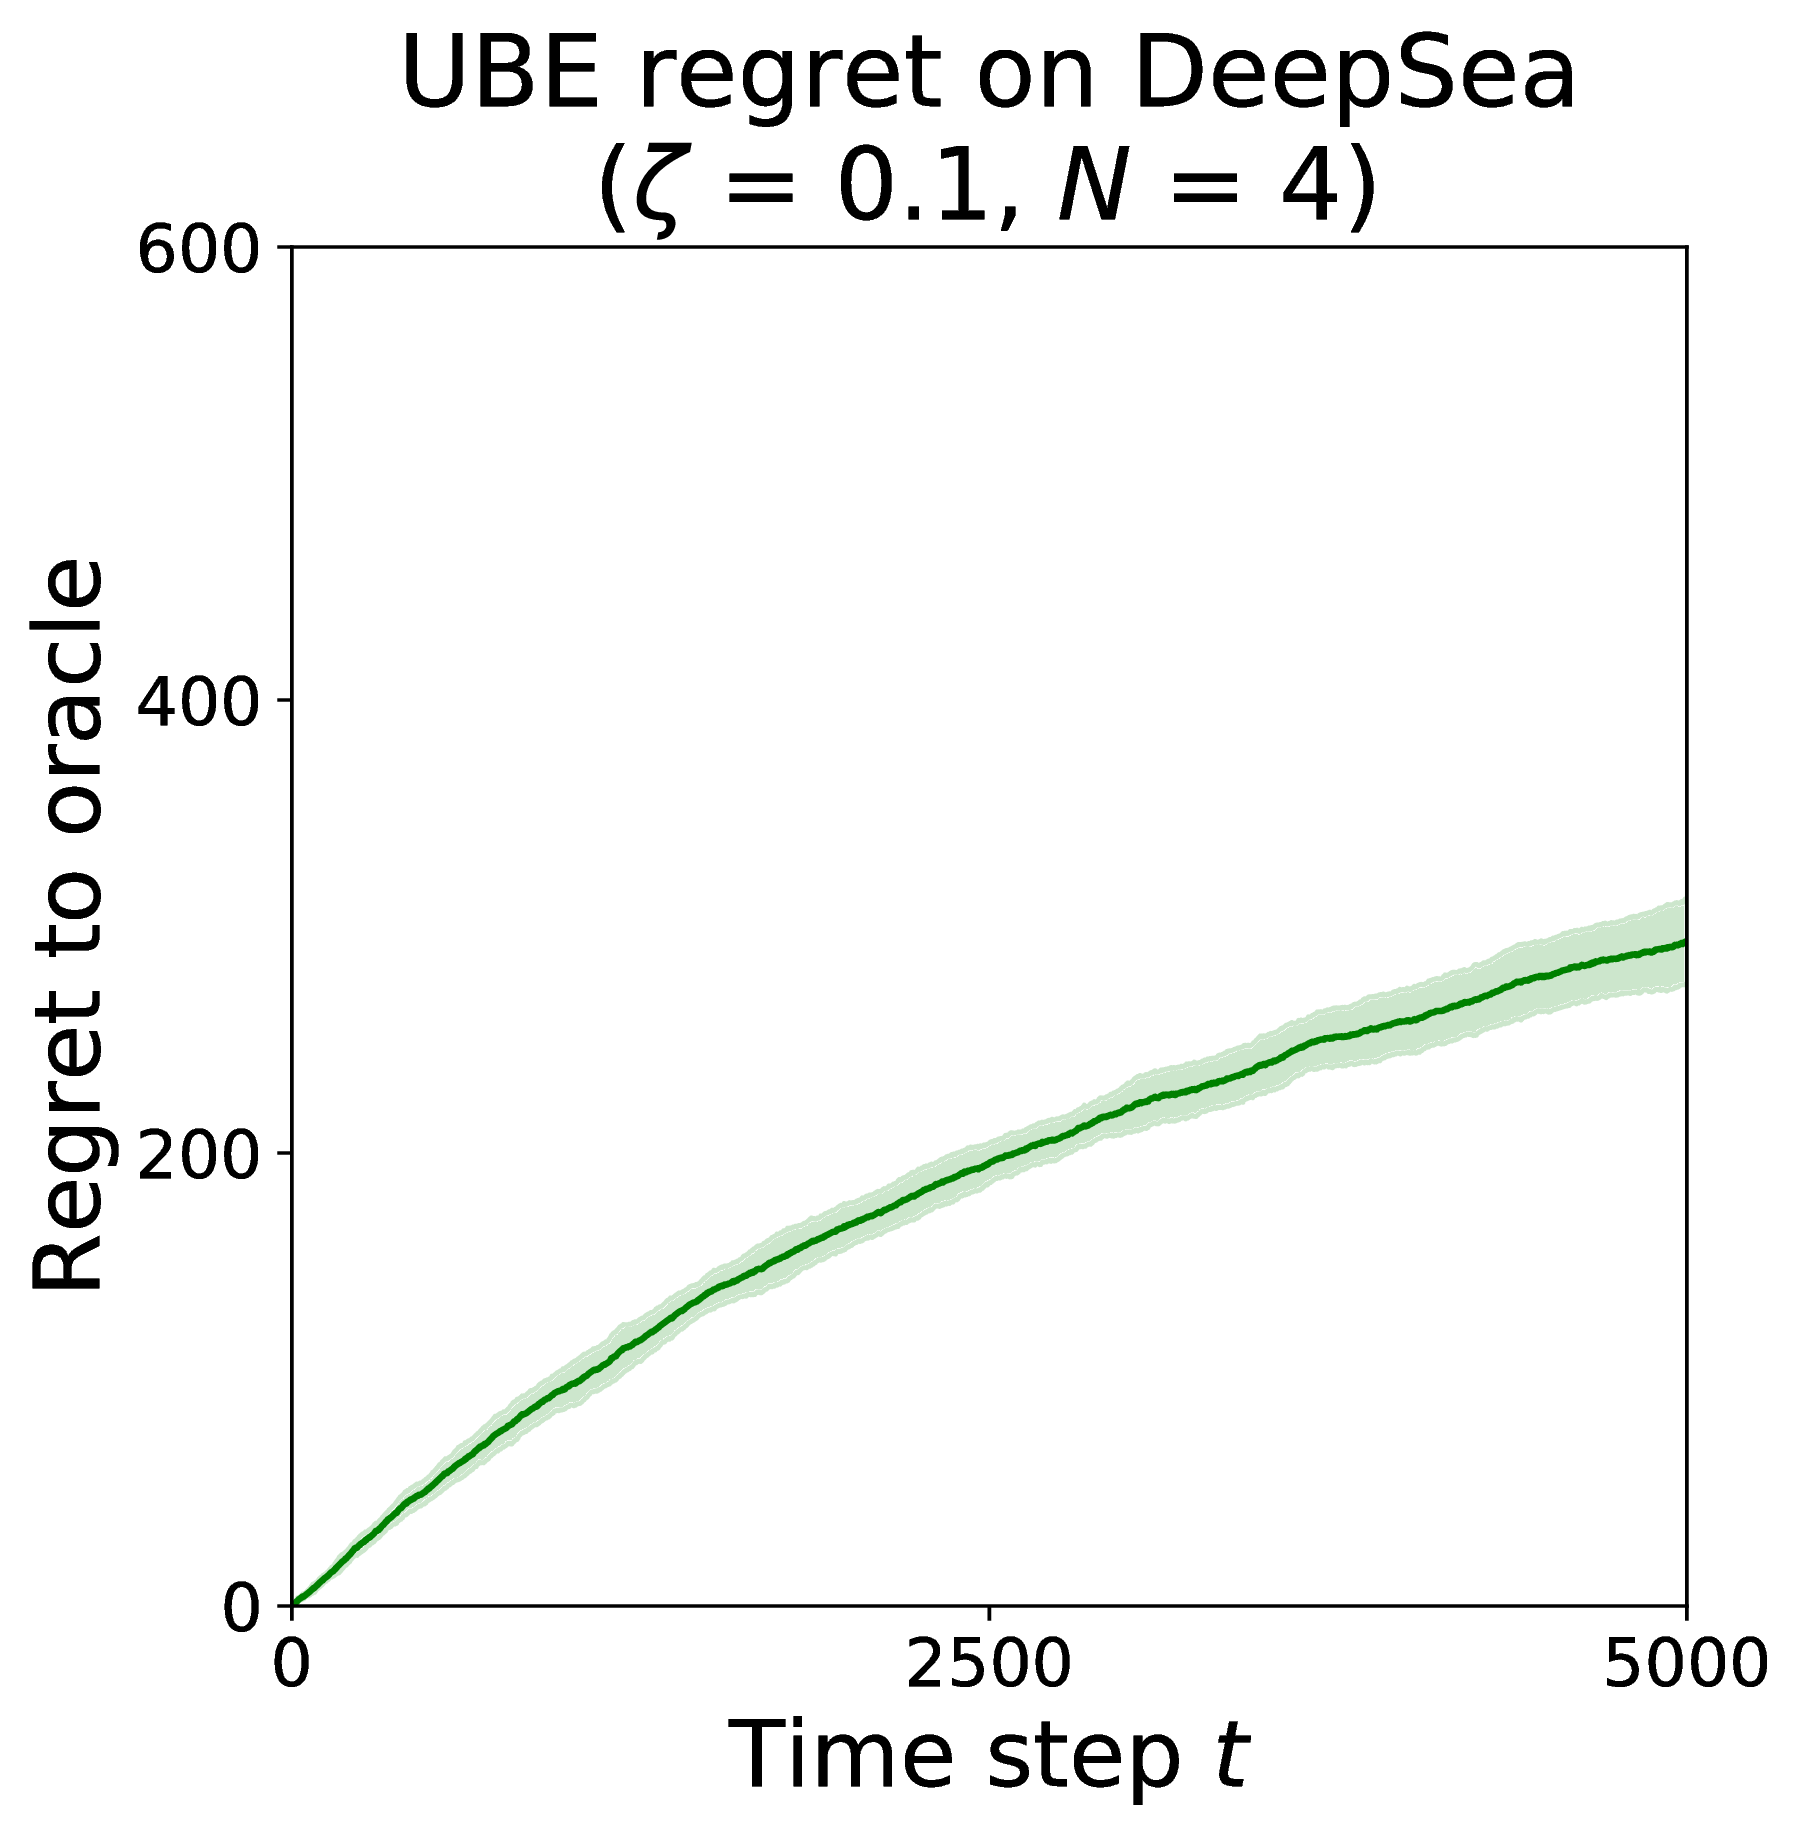
\includegraphics[width=\linewidth]{img/ube-0_0-4_0-3_0-3_0-0_1-regret-deepsea-4.pdf}~\\~\\
\end{subfigure}
\captionsetup{width=0.9\linewidth}
\caption{UBE posterior and regret on DeepSea.}\label{ube_deepsea_visual01}
\end{figure}

\begin{figure}[h!]
\centering
\begin{subfigure}{0.7\textwidth}
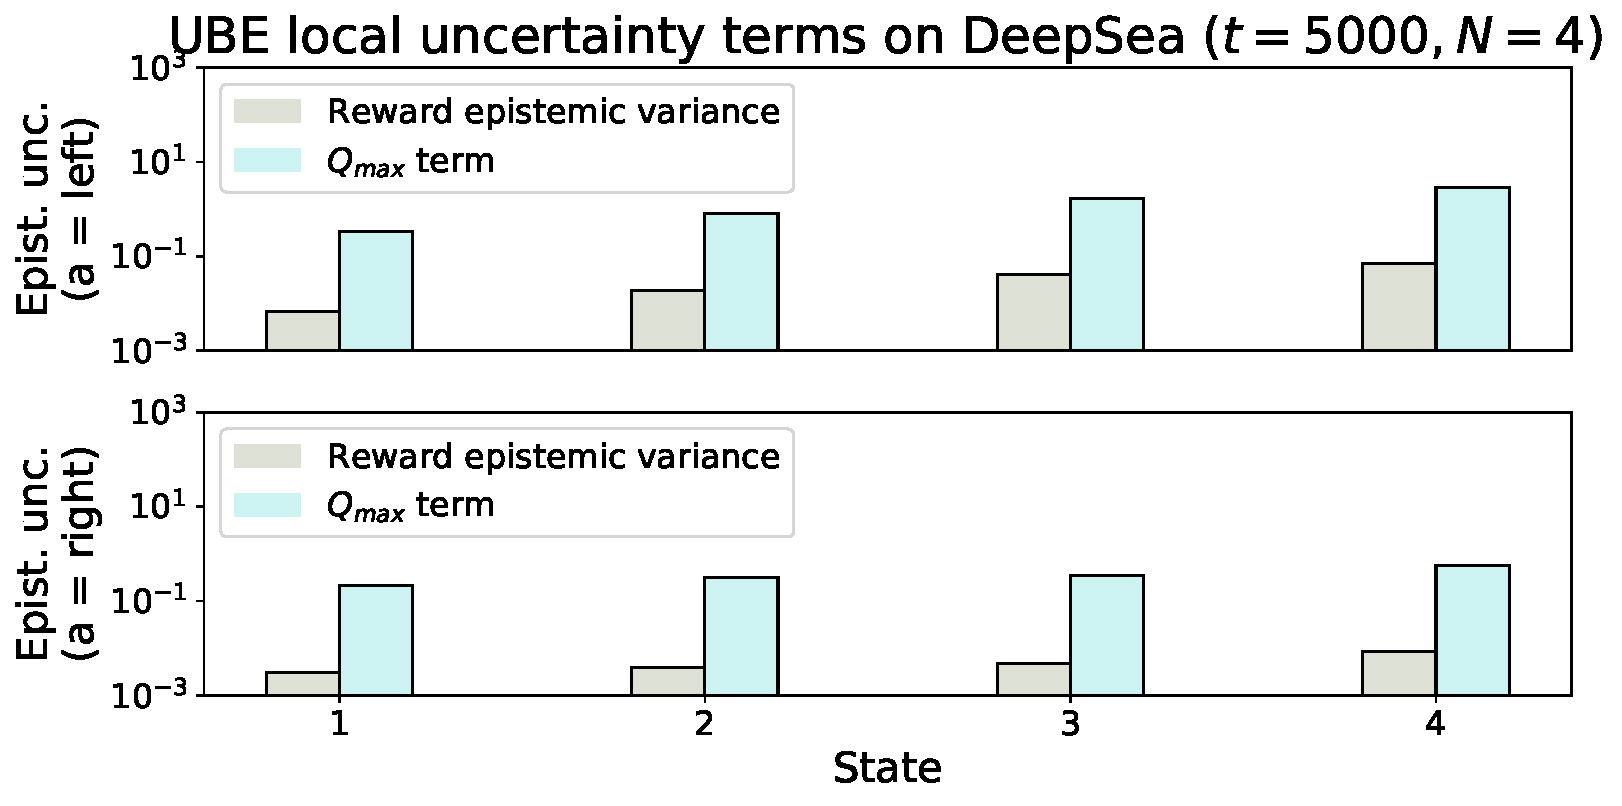
\includegraphics[width=\linewidth]{img/ube-uncertainty-terms.pdf}
\end{subfigure}
\captionsetup{width=0.9\linewidth}
\caption{Contributions to the local variance $\nu^*_{\s, \ac}$ by the reward and the $Q_{max}$ term. This plot corresponds to \cref{ube_deepsea_visual01}. Note the logarithmic scale.}\label{ube_unc_terms}
\end{figure}

\begin{figure}[h!]
\centering
\begin{subfigure}{0.65\textwidth}
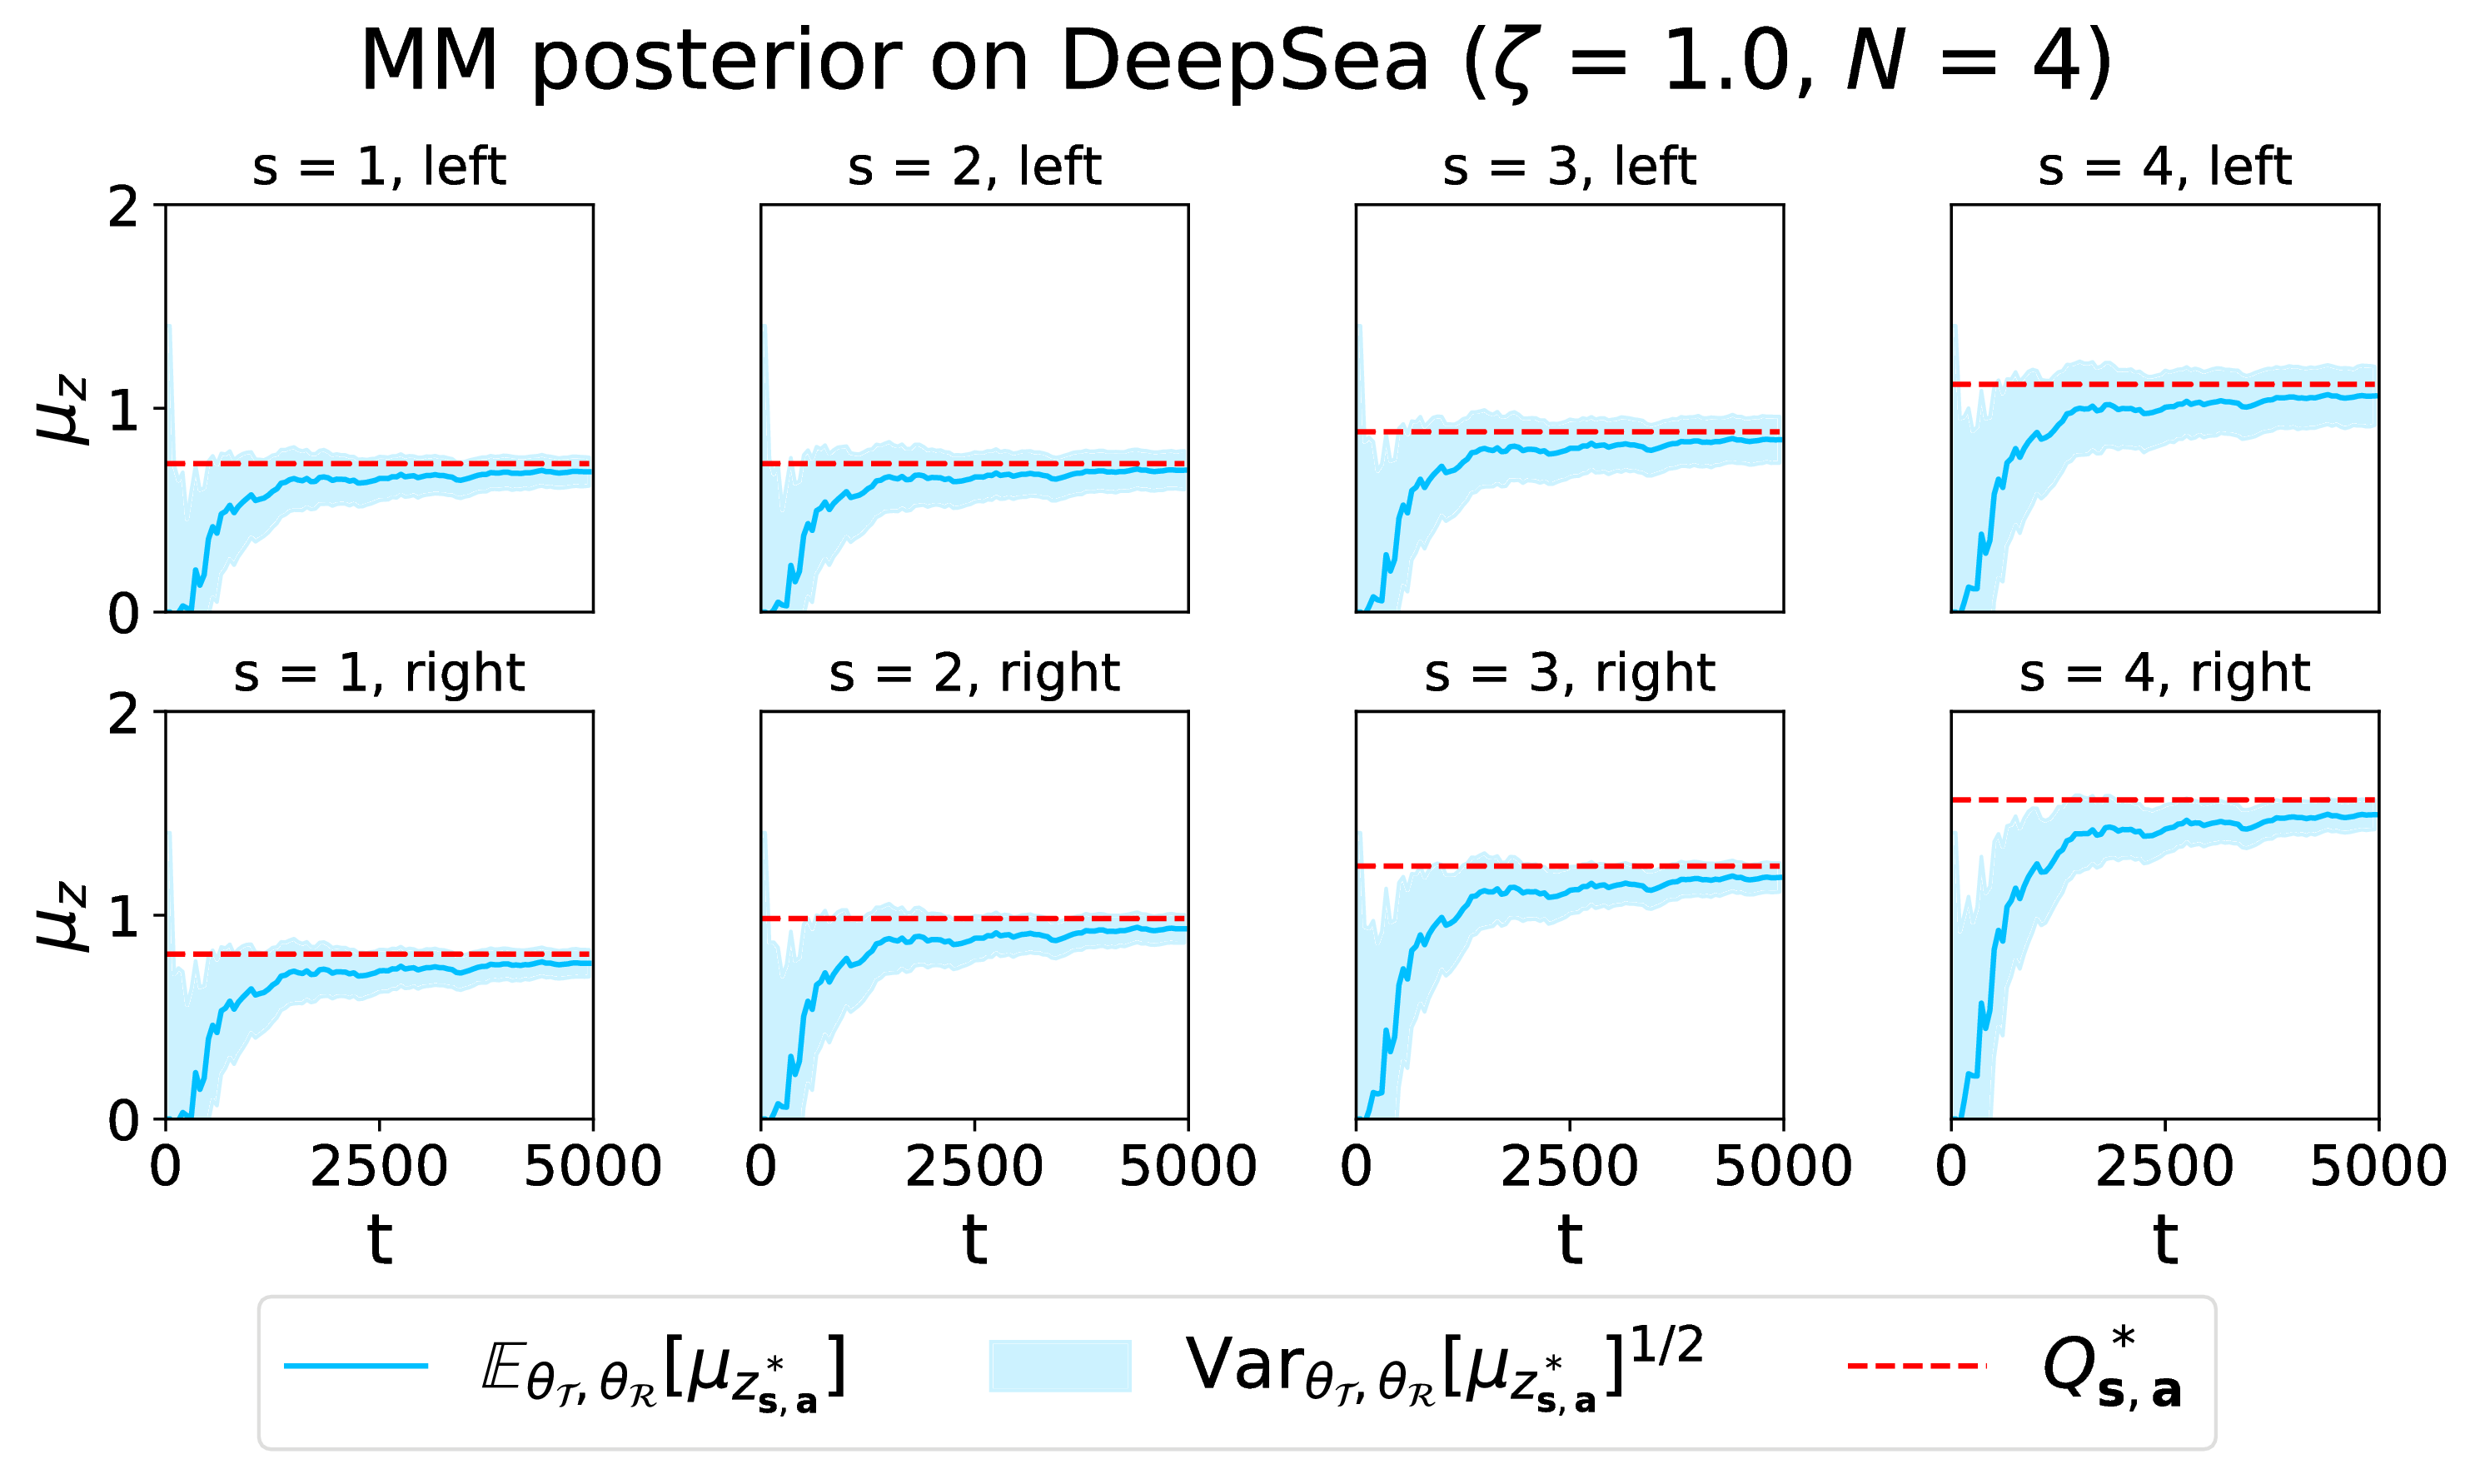
\includegraphics[width=\linewidth]{img/mm-0_0-4_0-3_0-3_0-1_0-posterior-deepsea-4.pdf}
\end{subfigure}
\begin{subfigure}{0.34\textwidth}
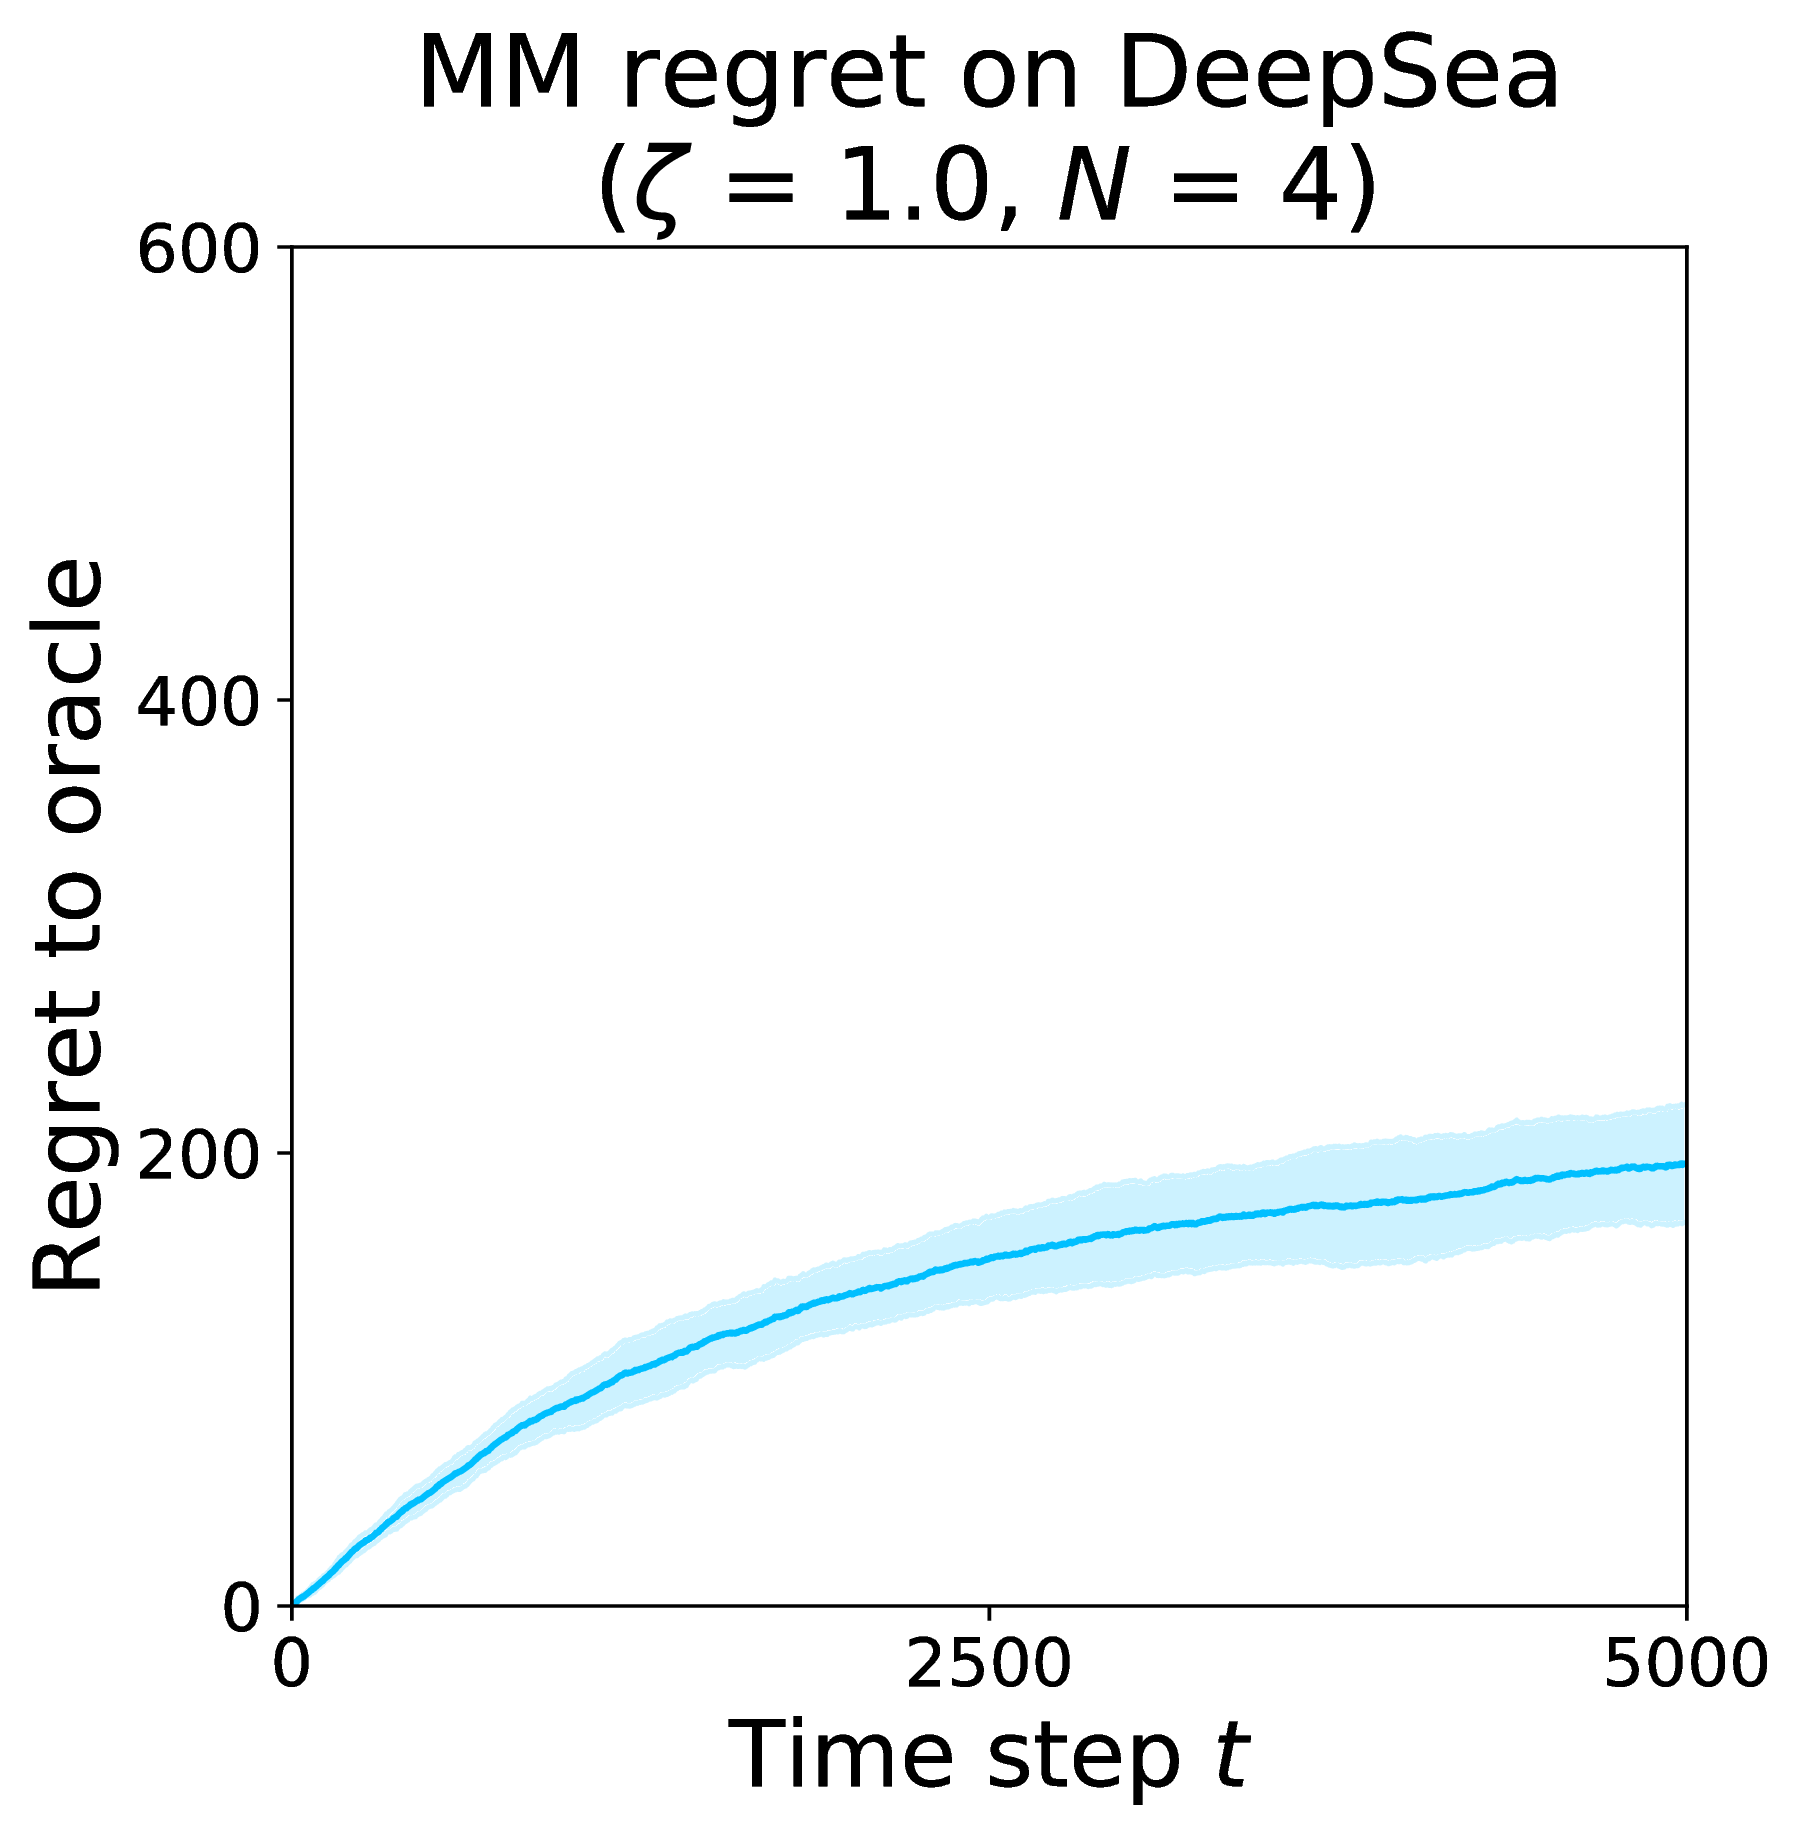
\includegraphics[width=\linewidth]{img/mm-0_0-4_0-3_0-3_0-1_0-regret-deepsea-4.pdf}~\\~\\
\end{subfigure}
\captionsetup{width=0.9\linewidth}
\caption{MM posterior and regret on DeepSea.}\label{mm_deepsea_visual}
\end{figure}

% ============================================================
% WideNarrow
% ============================================================
\clearpage

\subsection{WideNarrow}

\begin{figure}[h!]
\centering
\begin{subfigure}{0.65\textwidth}
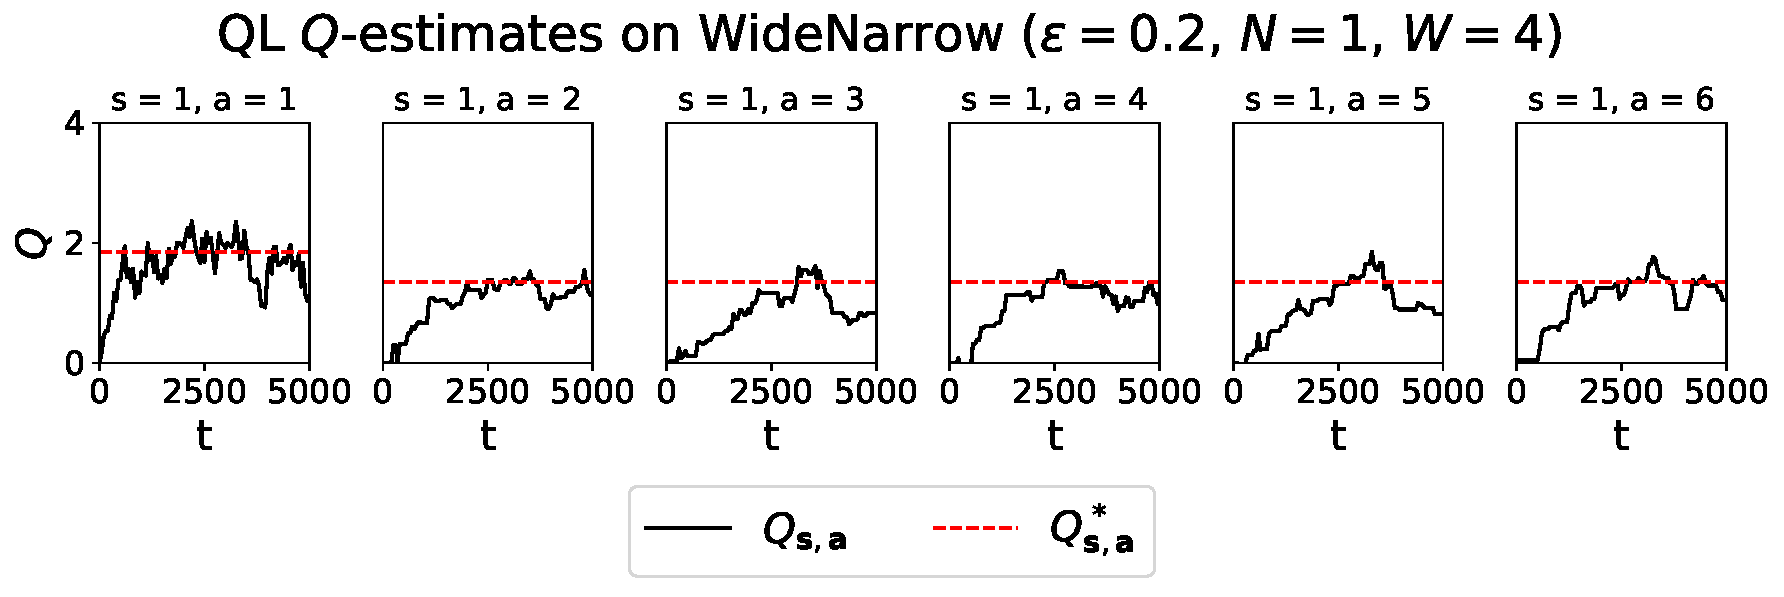
\includegraphics[width=\linewidth]{img/ql-0_2-qestimates-widenarrow-1-6.pdf}
\end{subfigure}
\begin{subfigure}{0.34\textwidth}
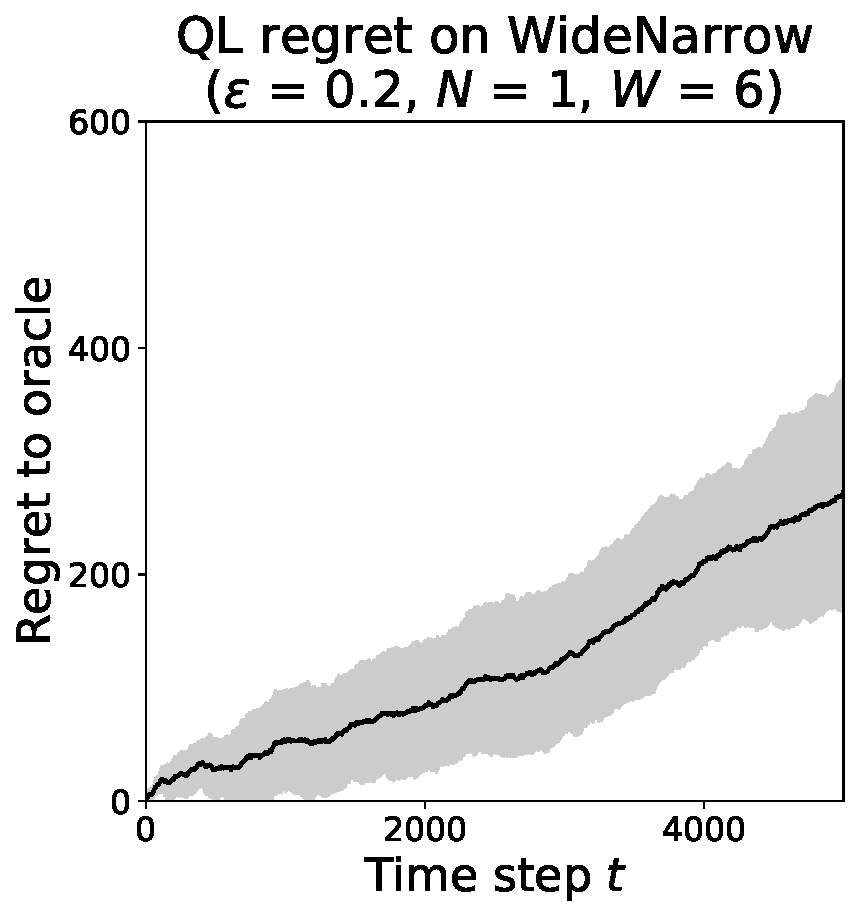
\includegraphics[width=\linewidth]{img/ql-0_2-regret-widenarrow-1-6.pdf}~\\~\\
\end{subfigure}
\captionsetup{width=0.9\linewidth}
\caption{QL $Q$-estimates and regret on WideNarrow.}\label{ql_widenarrow_visual}
\end{figure}

\begin{figure}[h!]
\centering
\begin{subfigure}{0.65\textwidth}
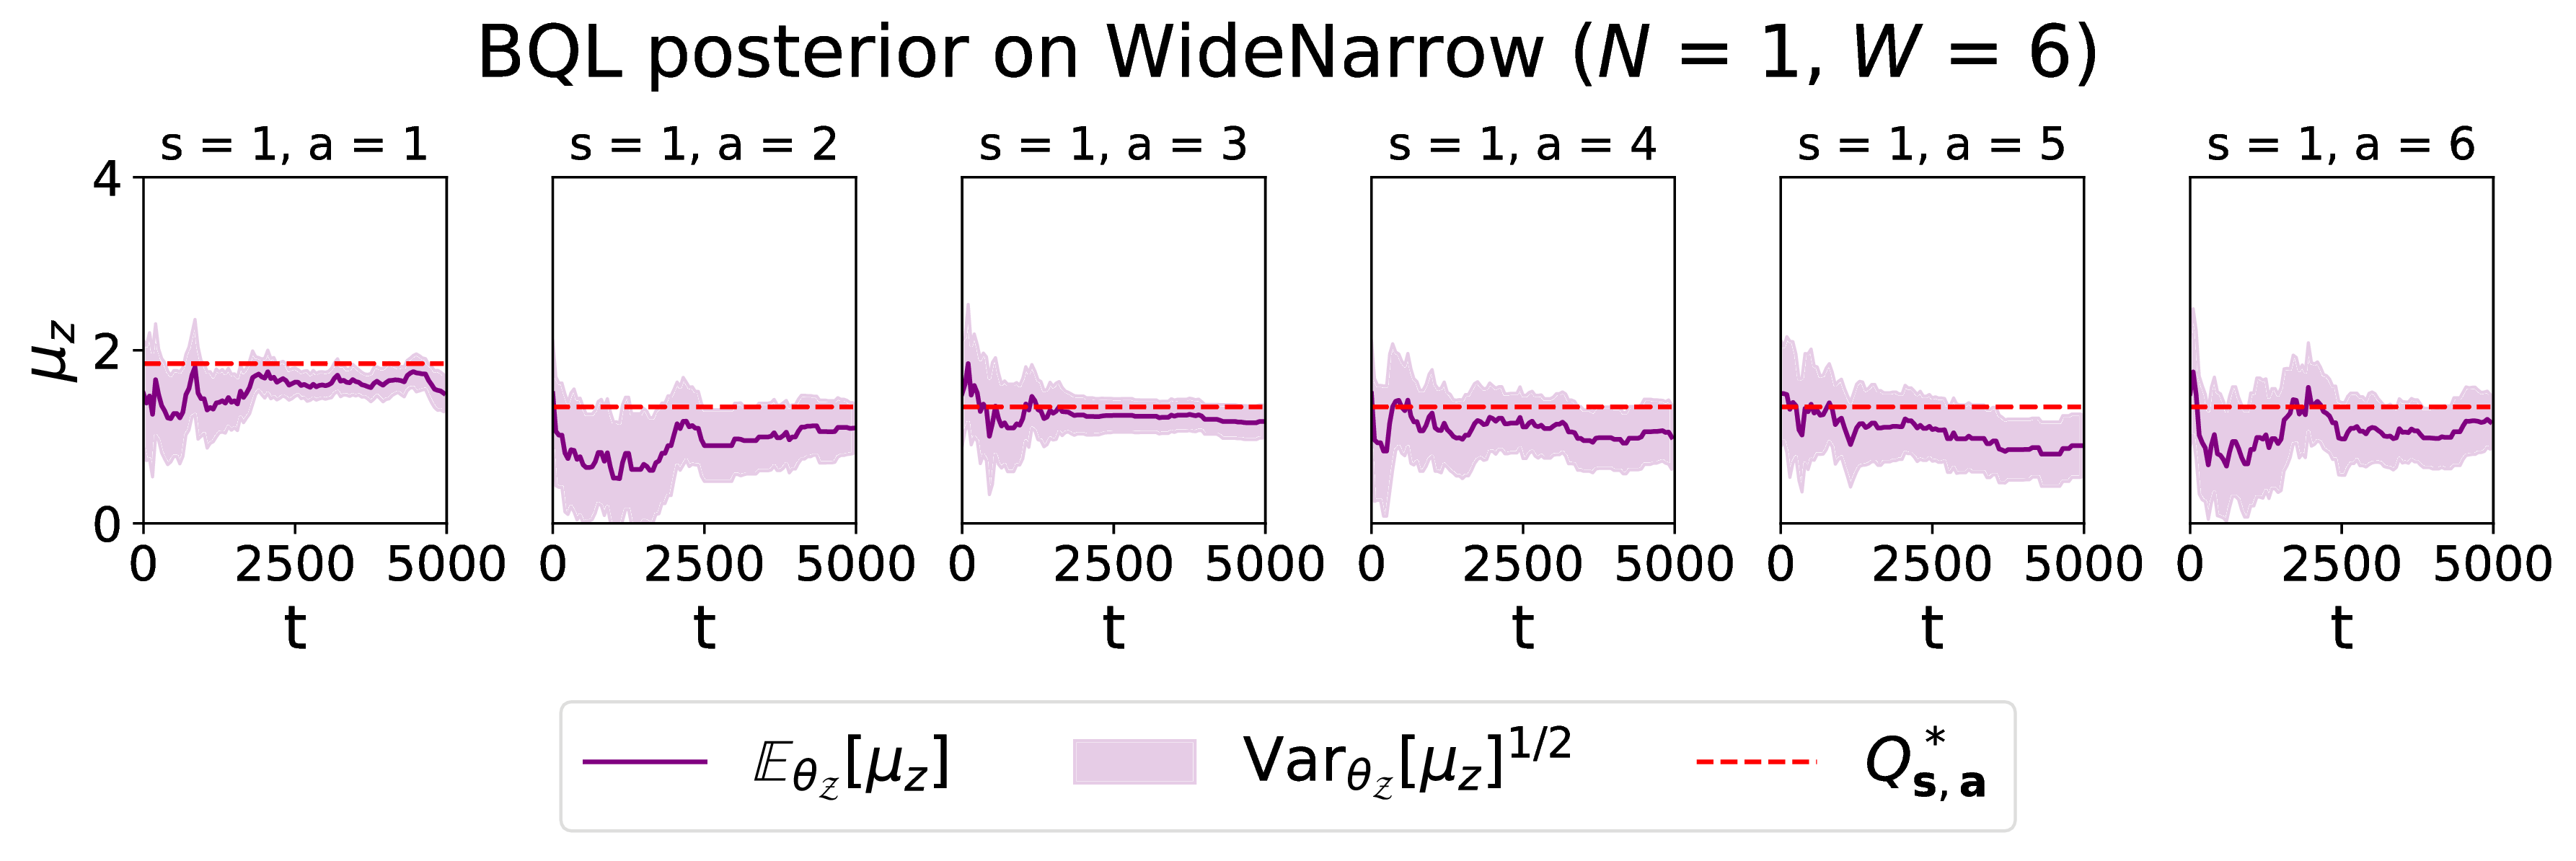
\includegraphics[width=\linewidth]{img/bql-1_5-4_0-3_0-3_0-posterior-widenarrow-1-6.pdf}
\end{subfigure}
\begin{subfigure}{0.34\textwidth}
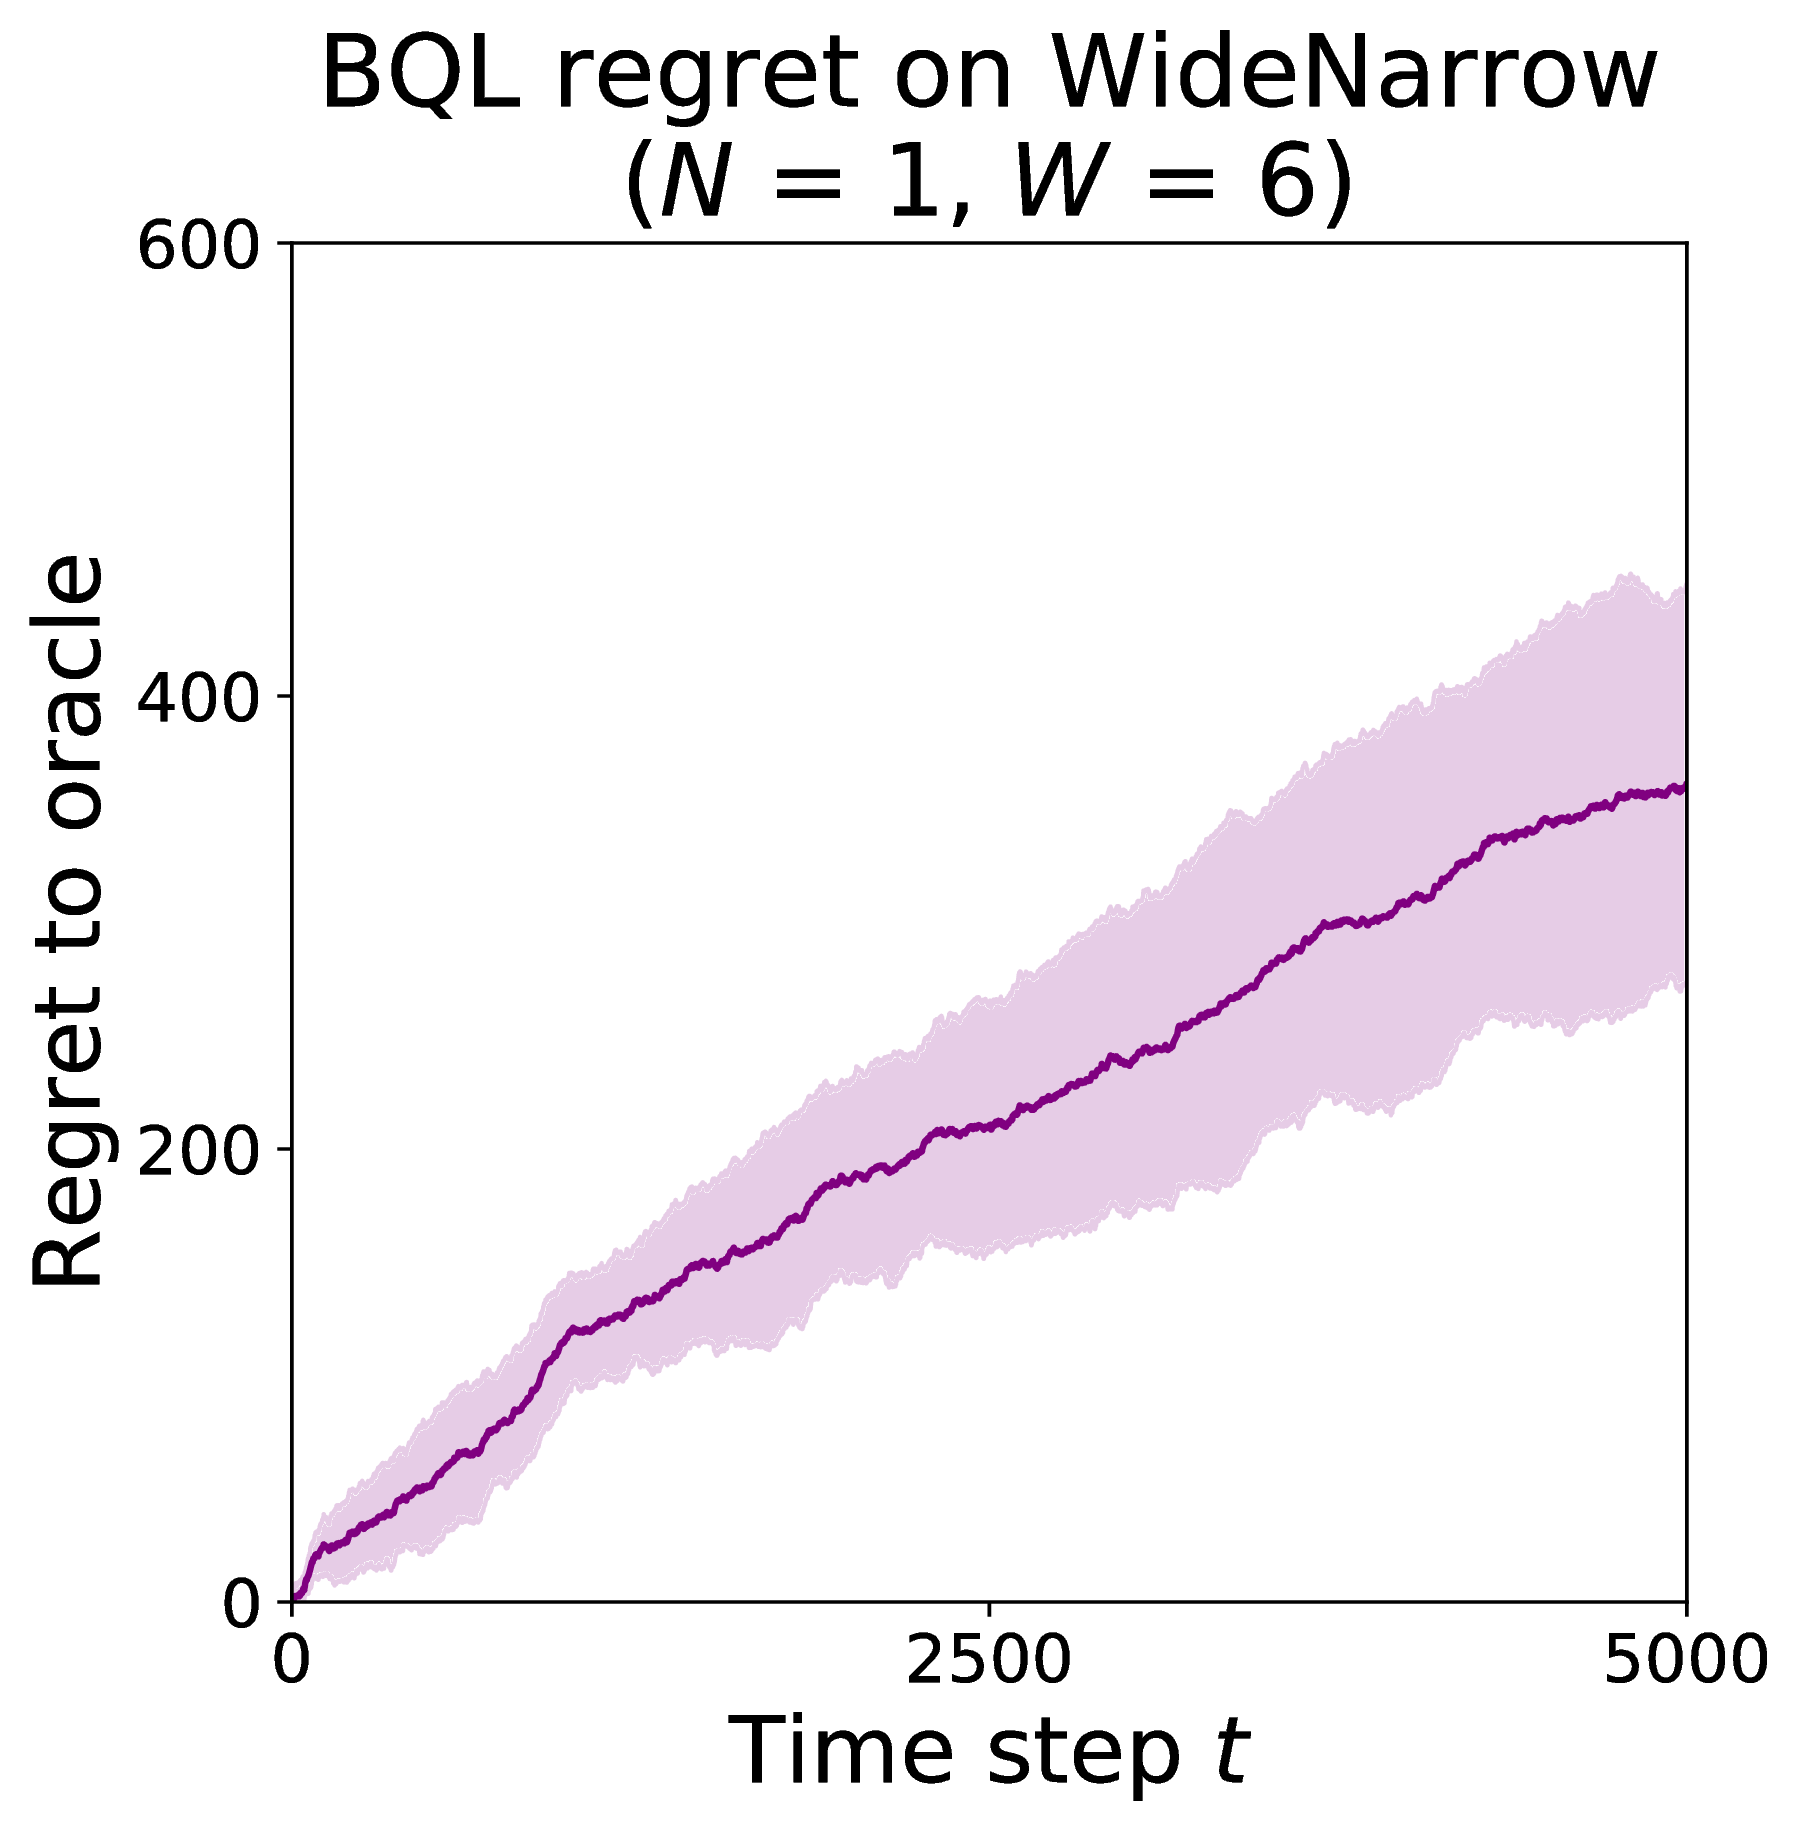
\includegraphics[width=\linewidth]{img/bql-1_5-4_0-3_0-3_0-regret-widenarrow-1-6.pdf}~\\~\\
\end{subfigure}
\captionsetup{width=0.9\linewidth}
\caption{BQL posterior and regret on WideNarrow.}\label{bql_widenarrow_visual}
\end{figure}

\begin{figure}[h!]
\centering
\begin{subfigure}{0.65\textwidth}
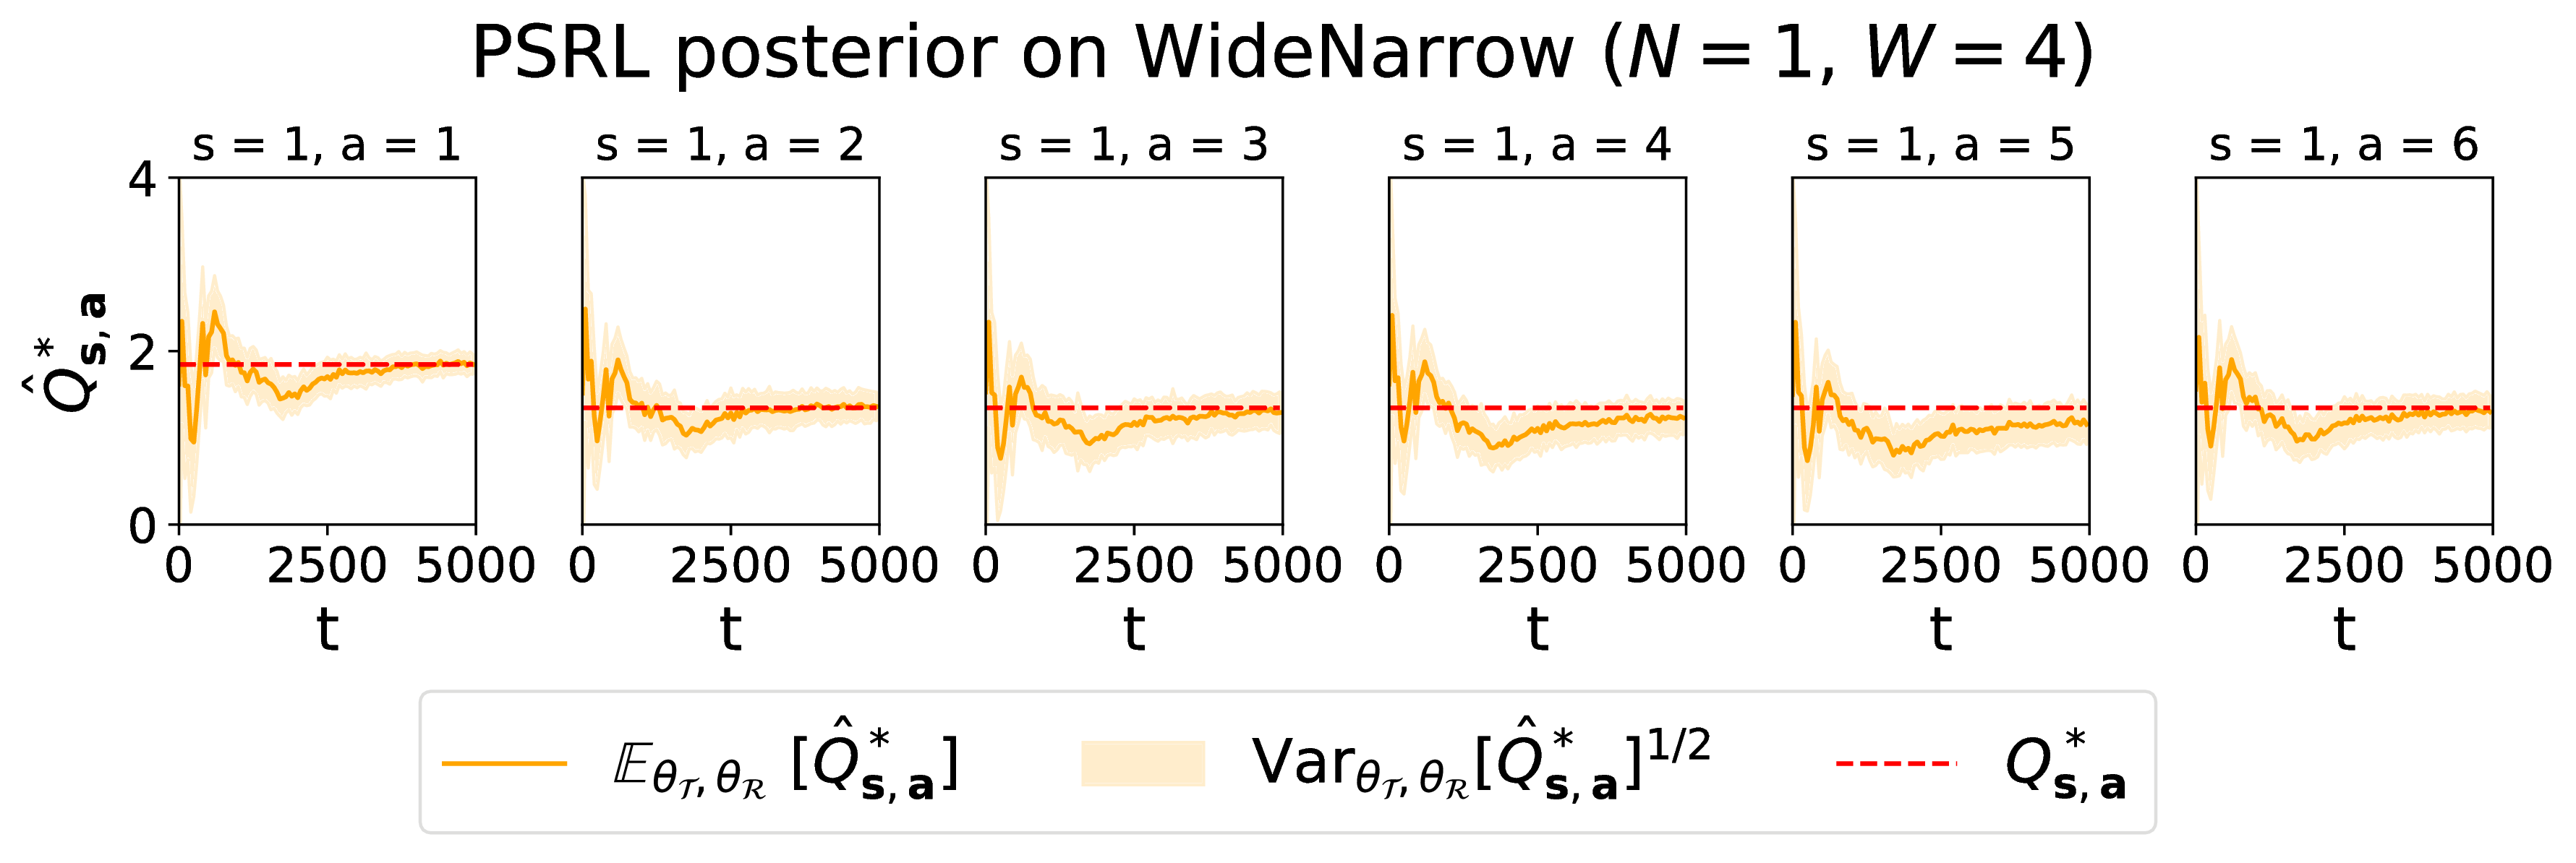
\includegraphics[width=\linewidth]{img/psrl-0_0-4_0-3_0-3_0-posterior-widenarrow-1-6.pdf}
\end{subfigure}
\begin{subfigure}{0.34\textwidth}
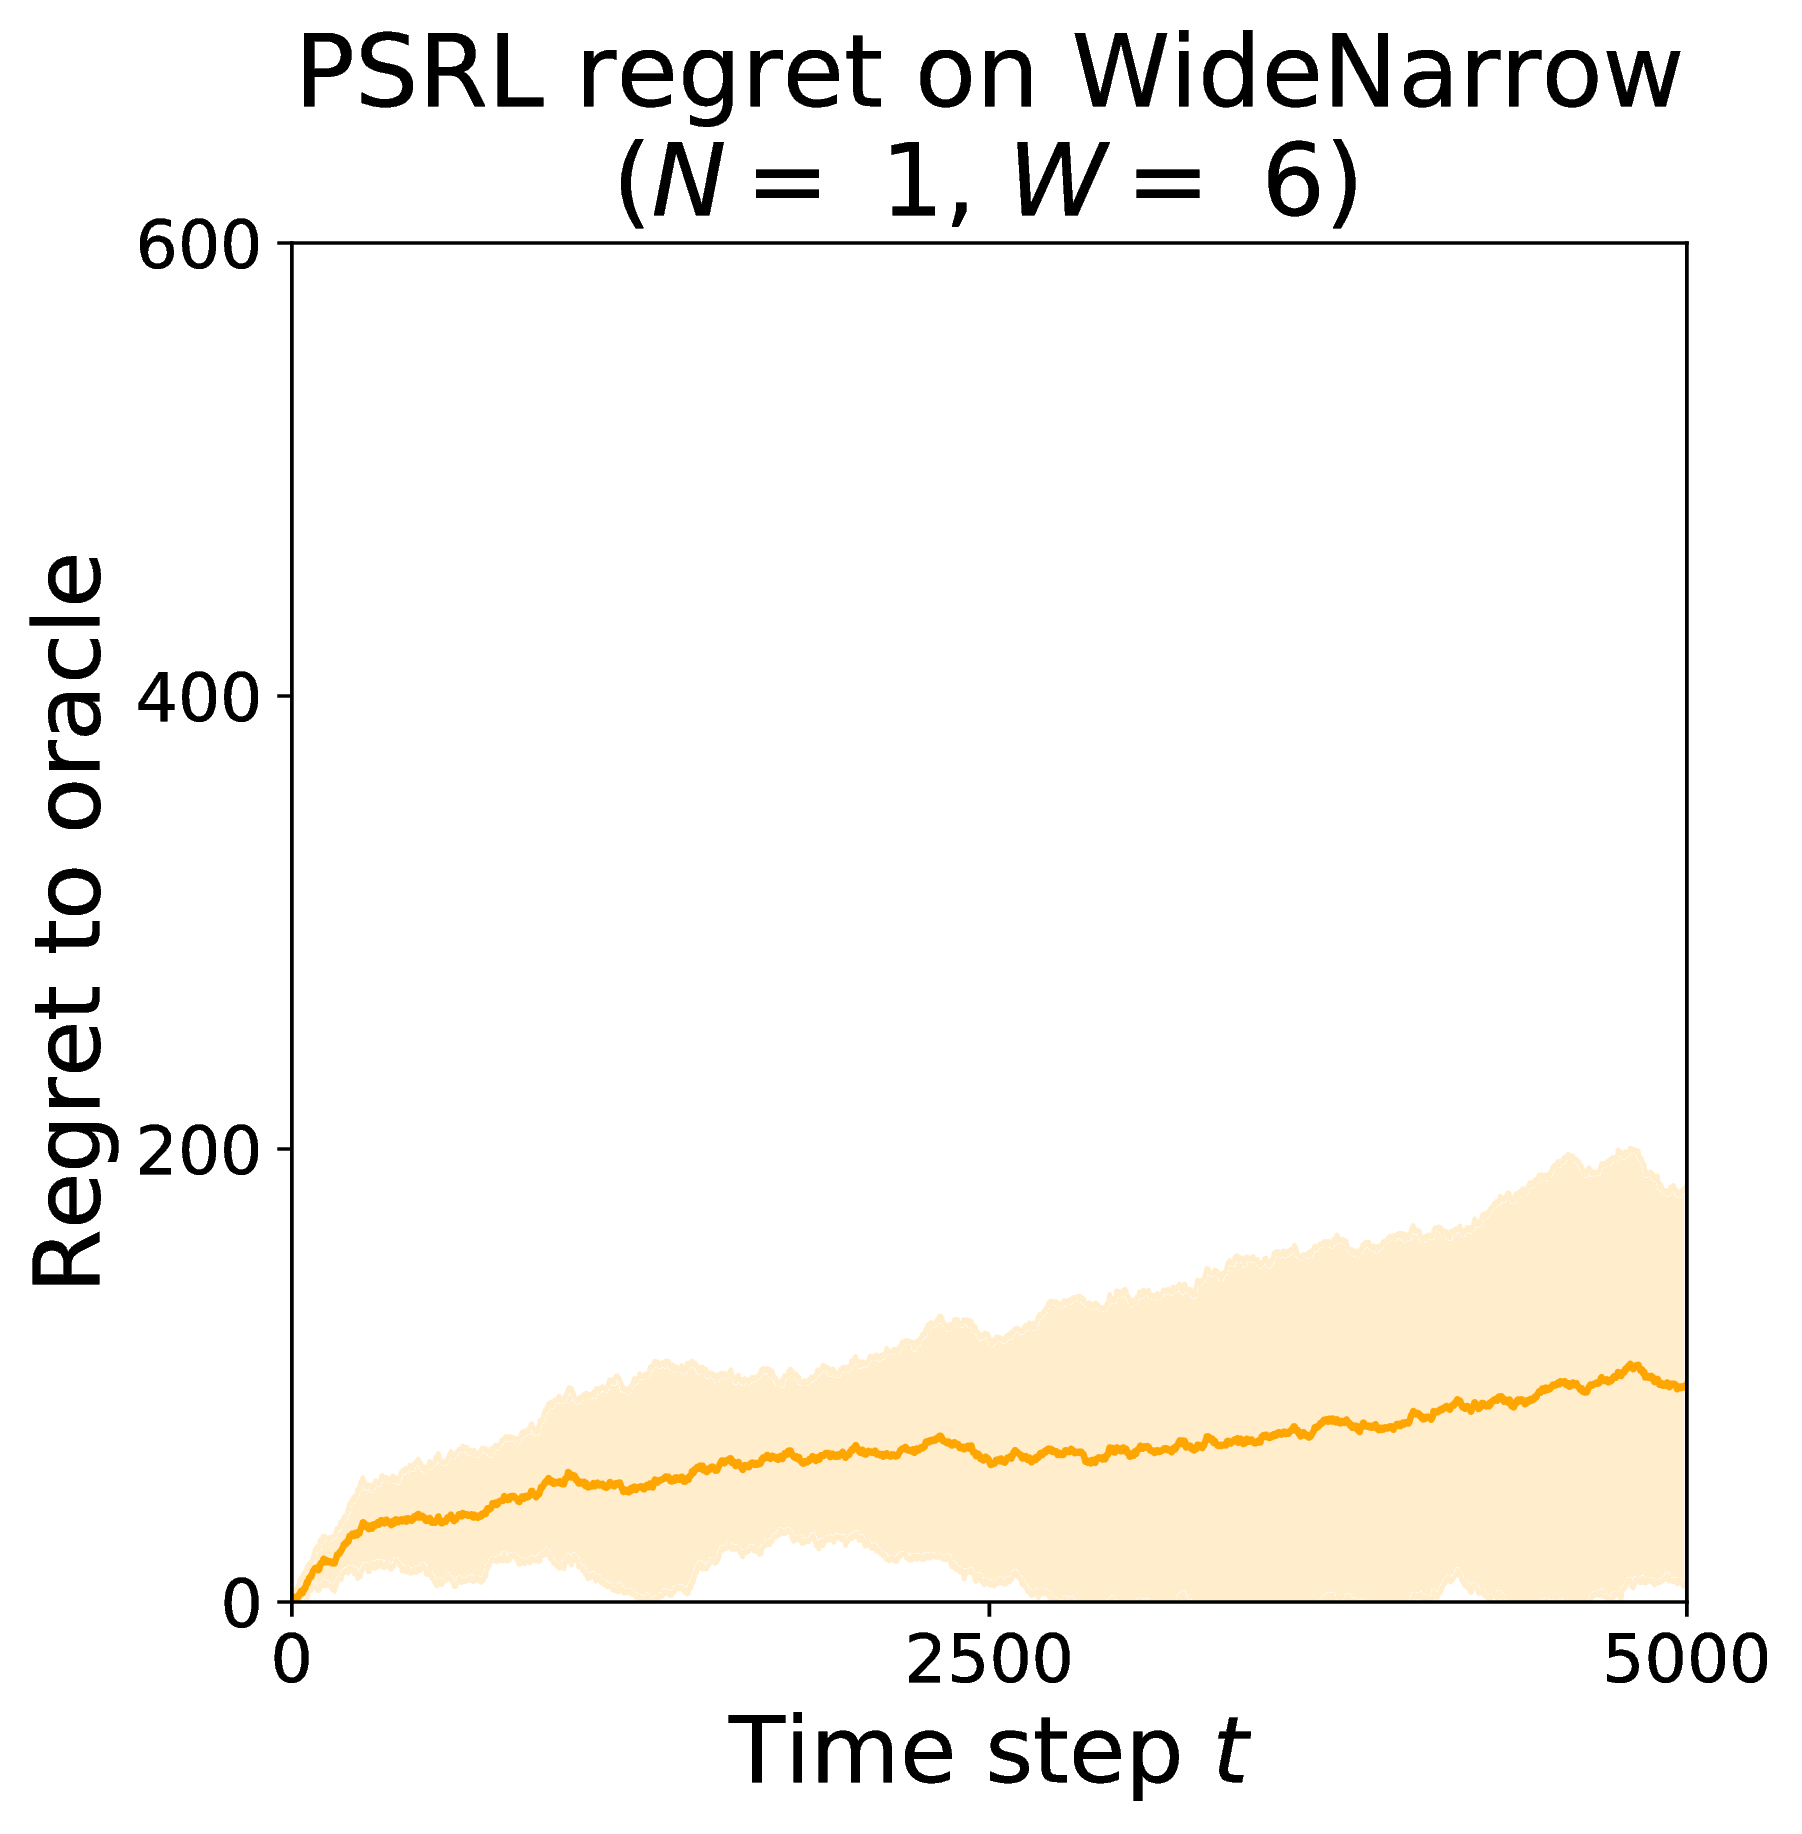
\includegraphics[width=\linewidth]{img/psrl-0_0-4_0-3_0-3_0-regret-widenarrow-1-6.pdf}~\\~\\
\end{subfigure}
\captionsetup{width=0.9\linewidth}
\caption{PSRL posterior and regret on WideNarrow.}\label{psrl_widenarrow_visual}
\end{figure}

\begin{figure}[h!]
\centering
\begin{subfigure}{0.65\textwidth}
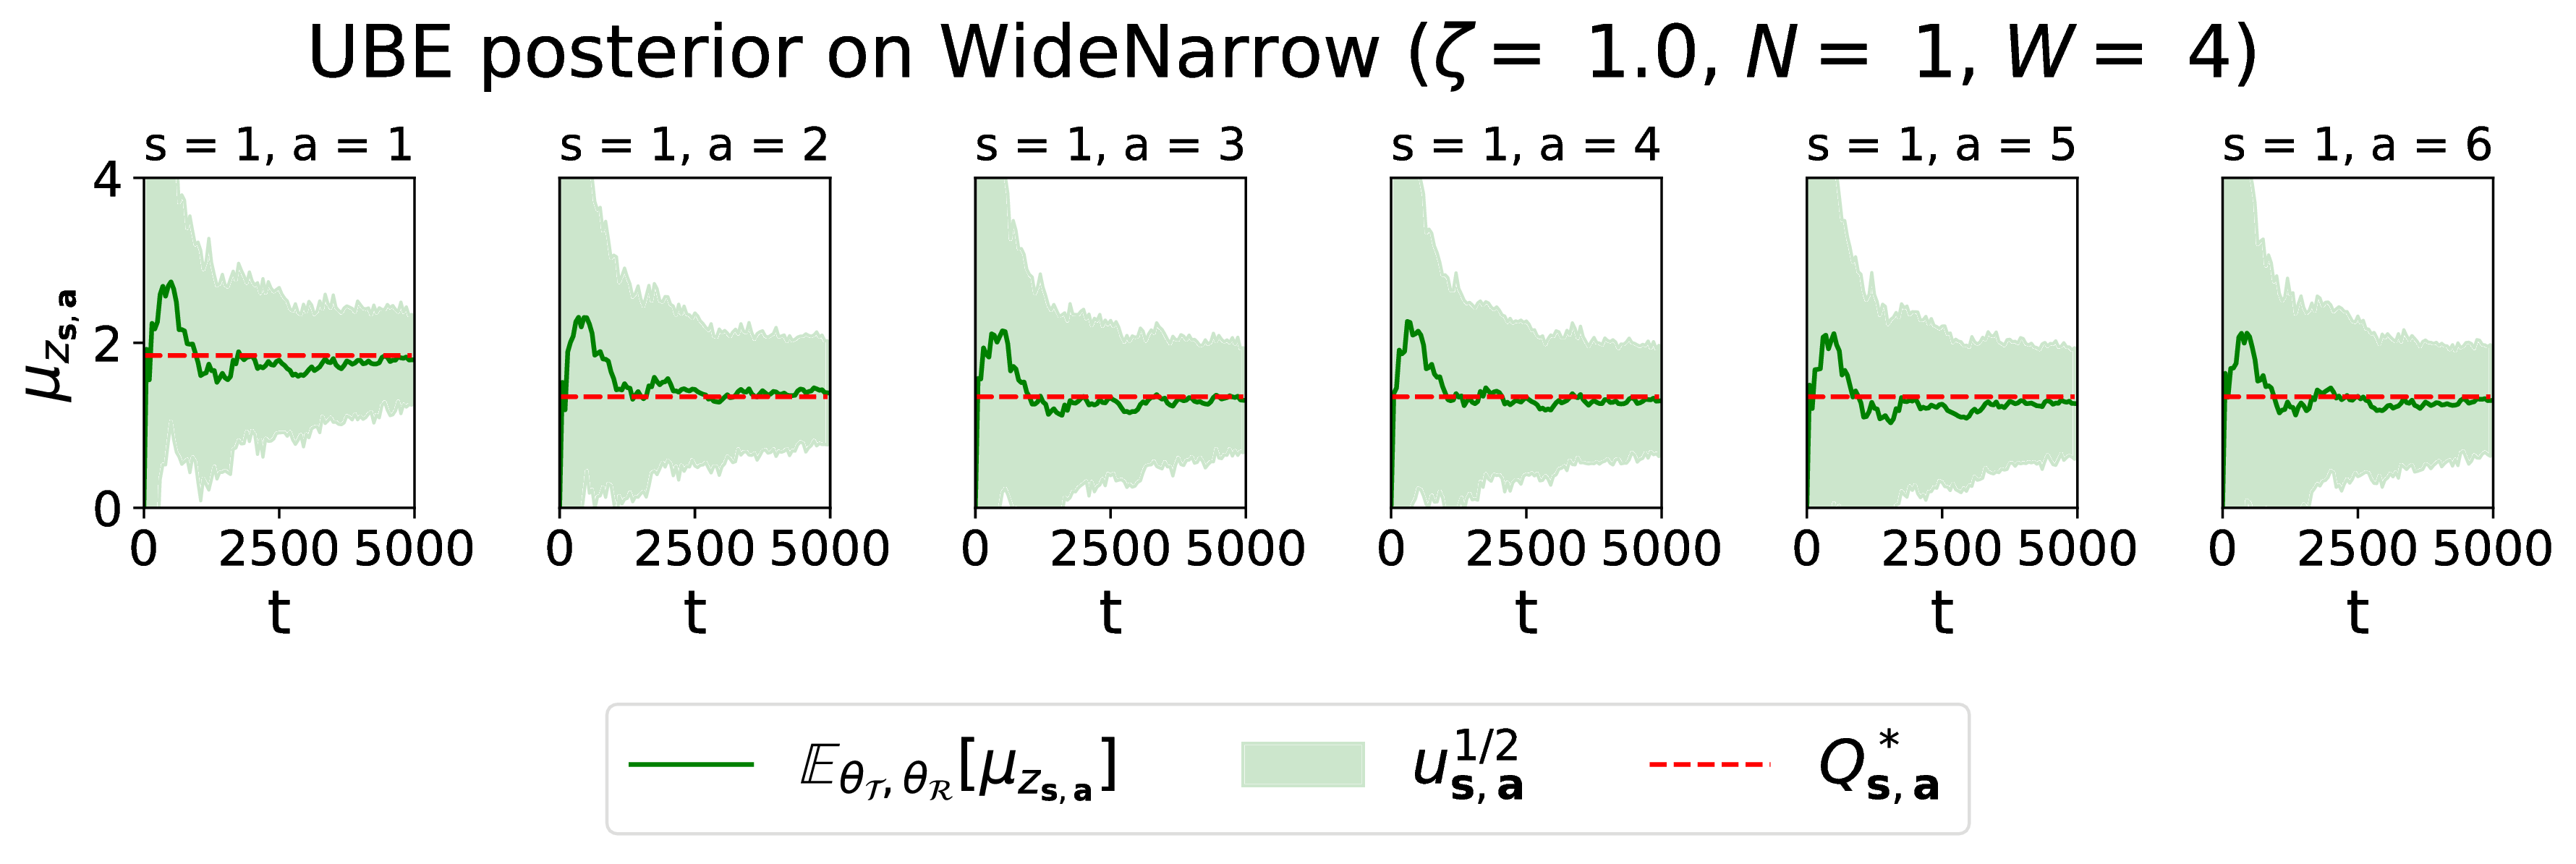
\includegraphics[width=\linewidth]{img/ube-0_0-4_0-3_0-3_0-1_0-posterior-widenarrow-1-6.pdf}
\end{subfigure}
\begin{subfigure}{0.34\textwidth}
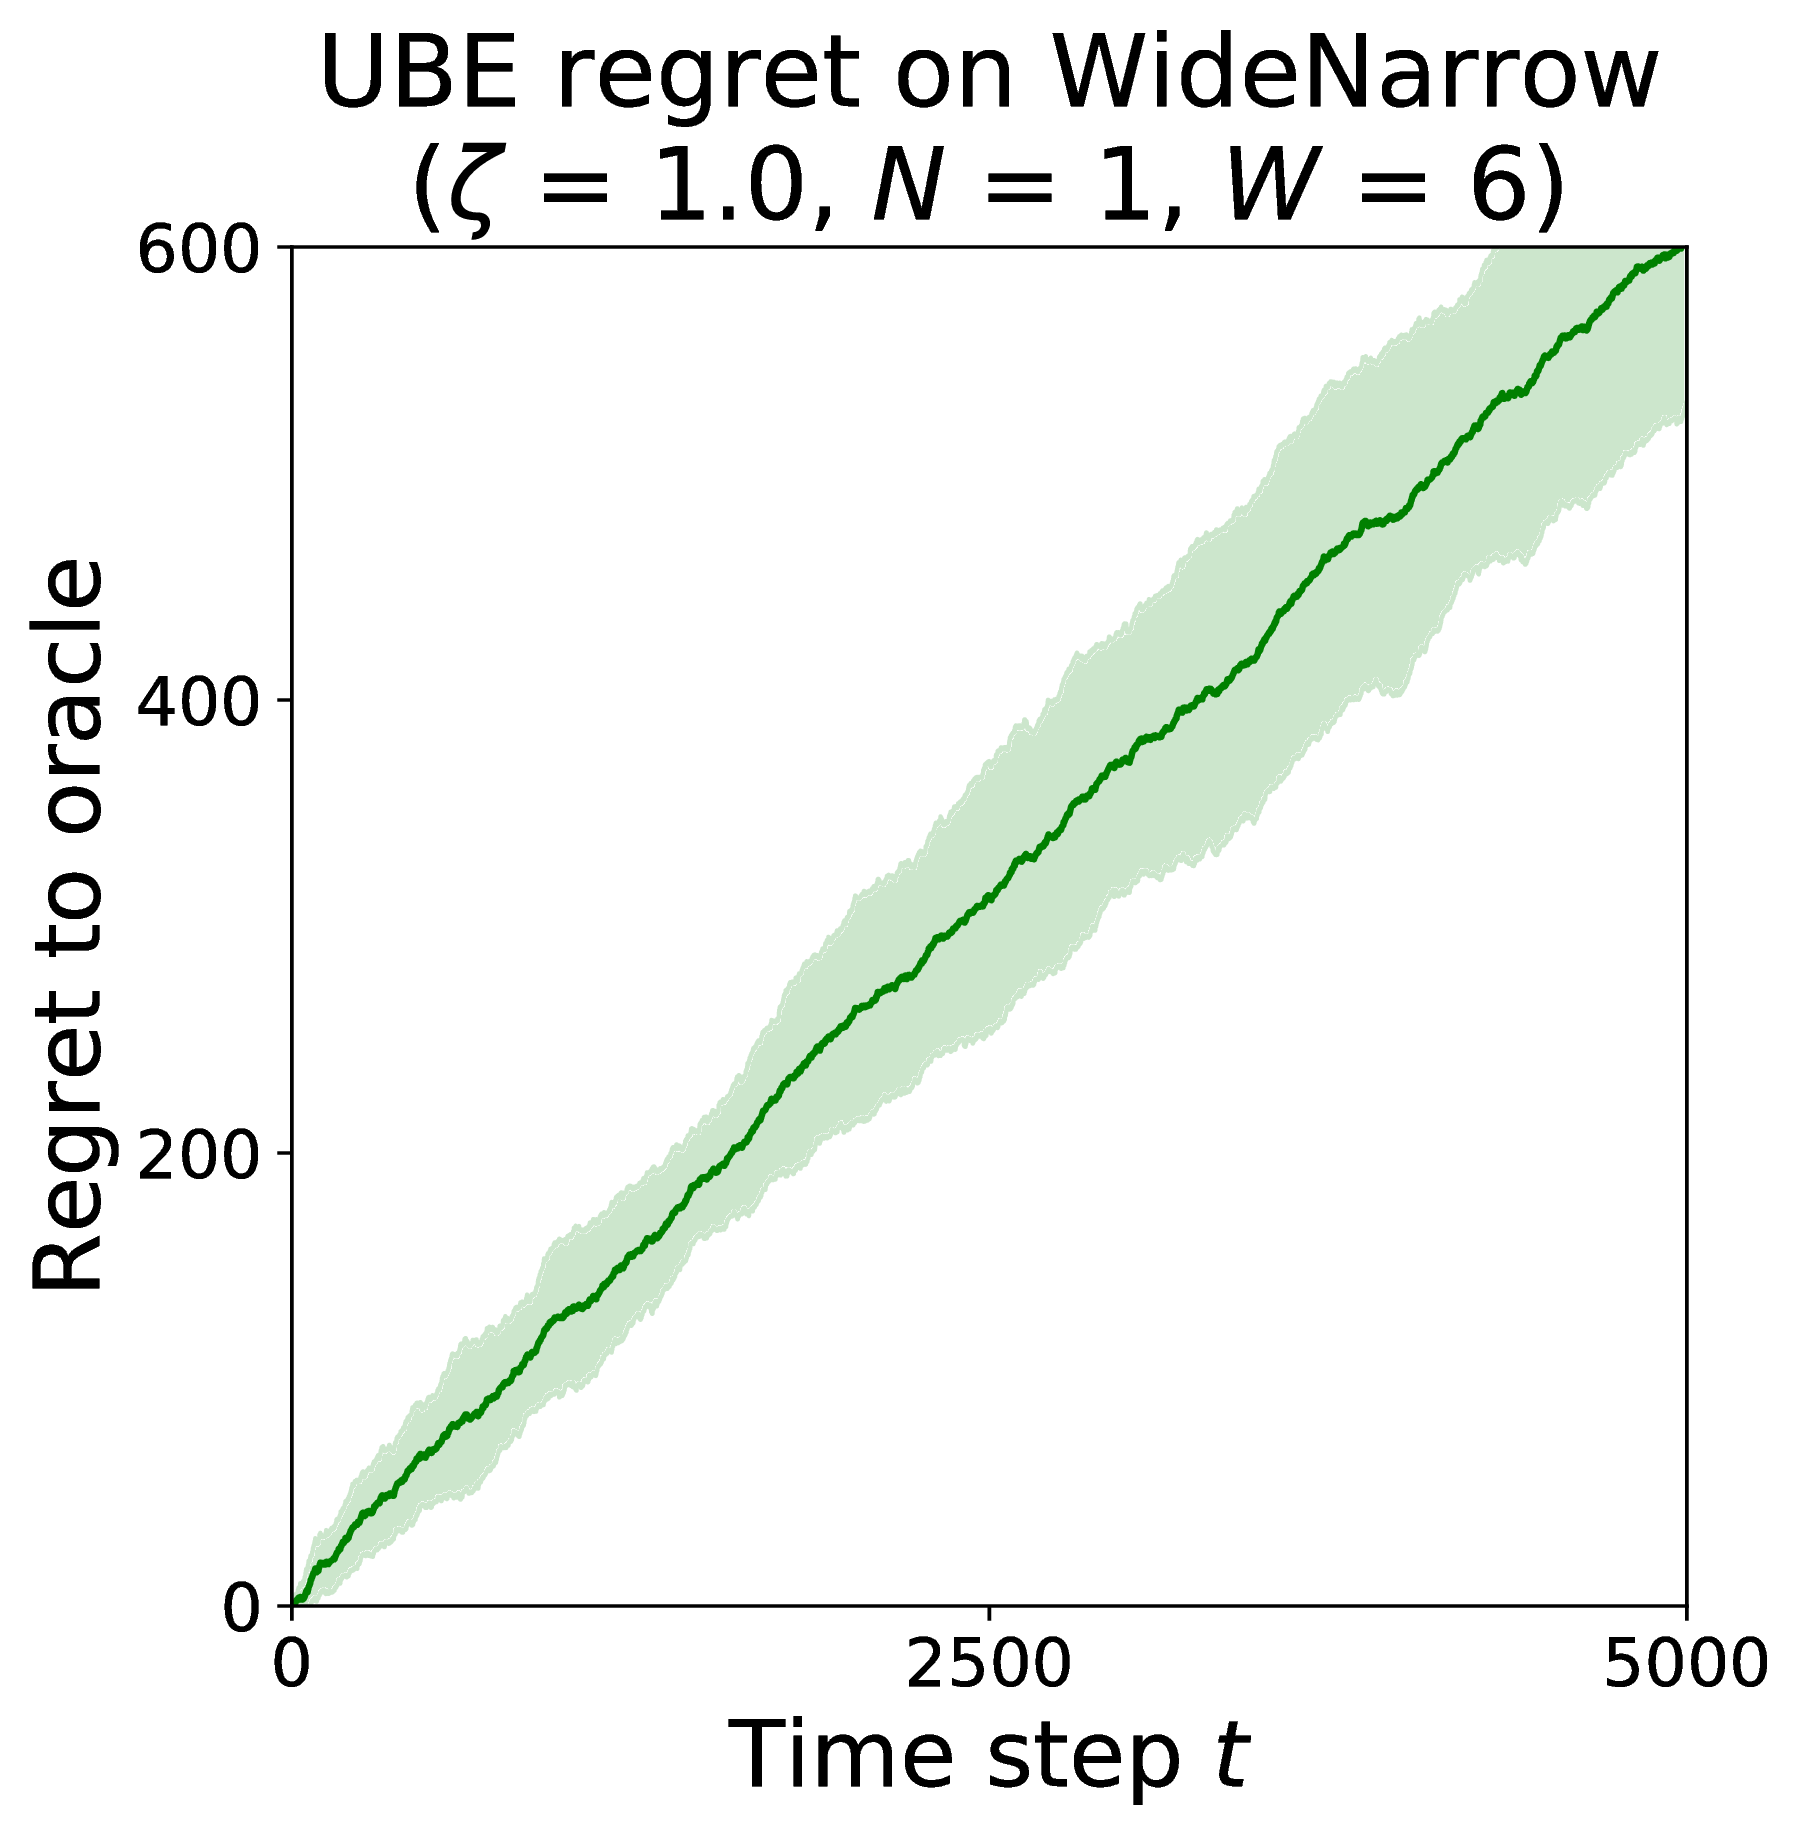
\includegraphics[width=\linewidth]{img/ube-0_0-4_0-3_0-3_0-1_0-regret-widenarrow-1-6.pdf}~\\~\\
\end{subfigure}
\captionsetup{width=0.9\linewidth}
\caption{UBE posterior and regret on WideNarrow.}\label{ube_widenarrow_visual1}
\end{figure}

\begin{figure}[h!]
\centering
\vspace{-1cm}
\begin{subfigure}{0.65\textwidth}
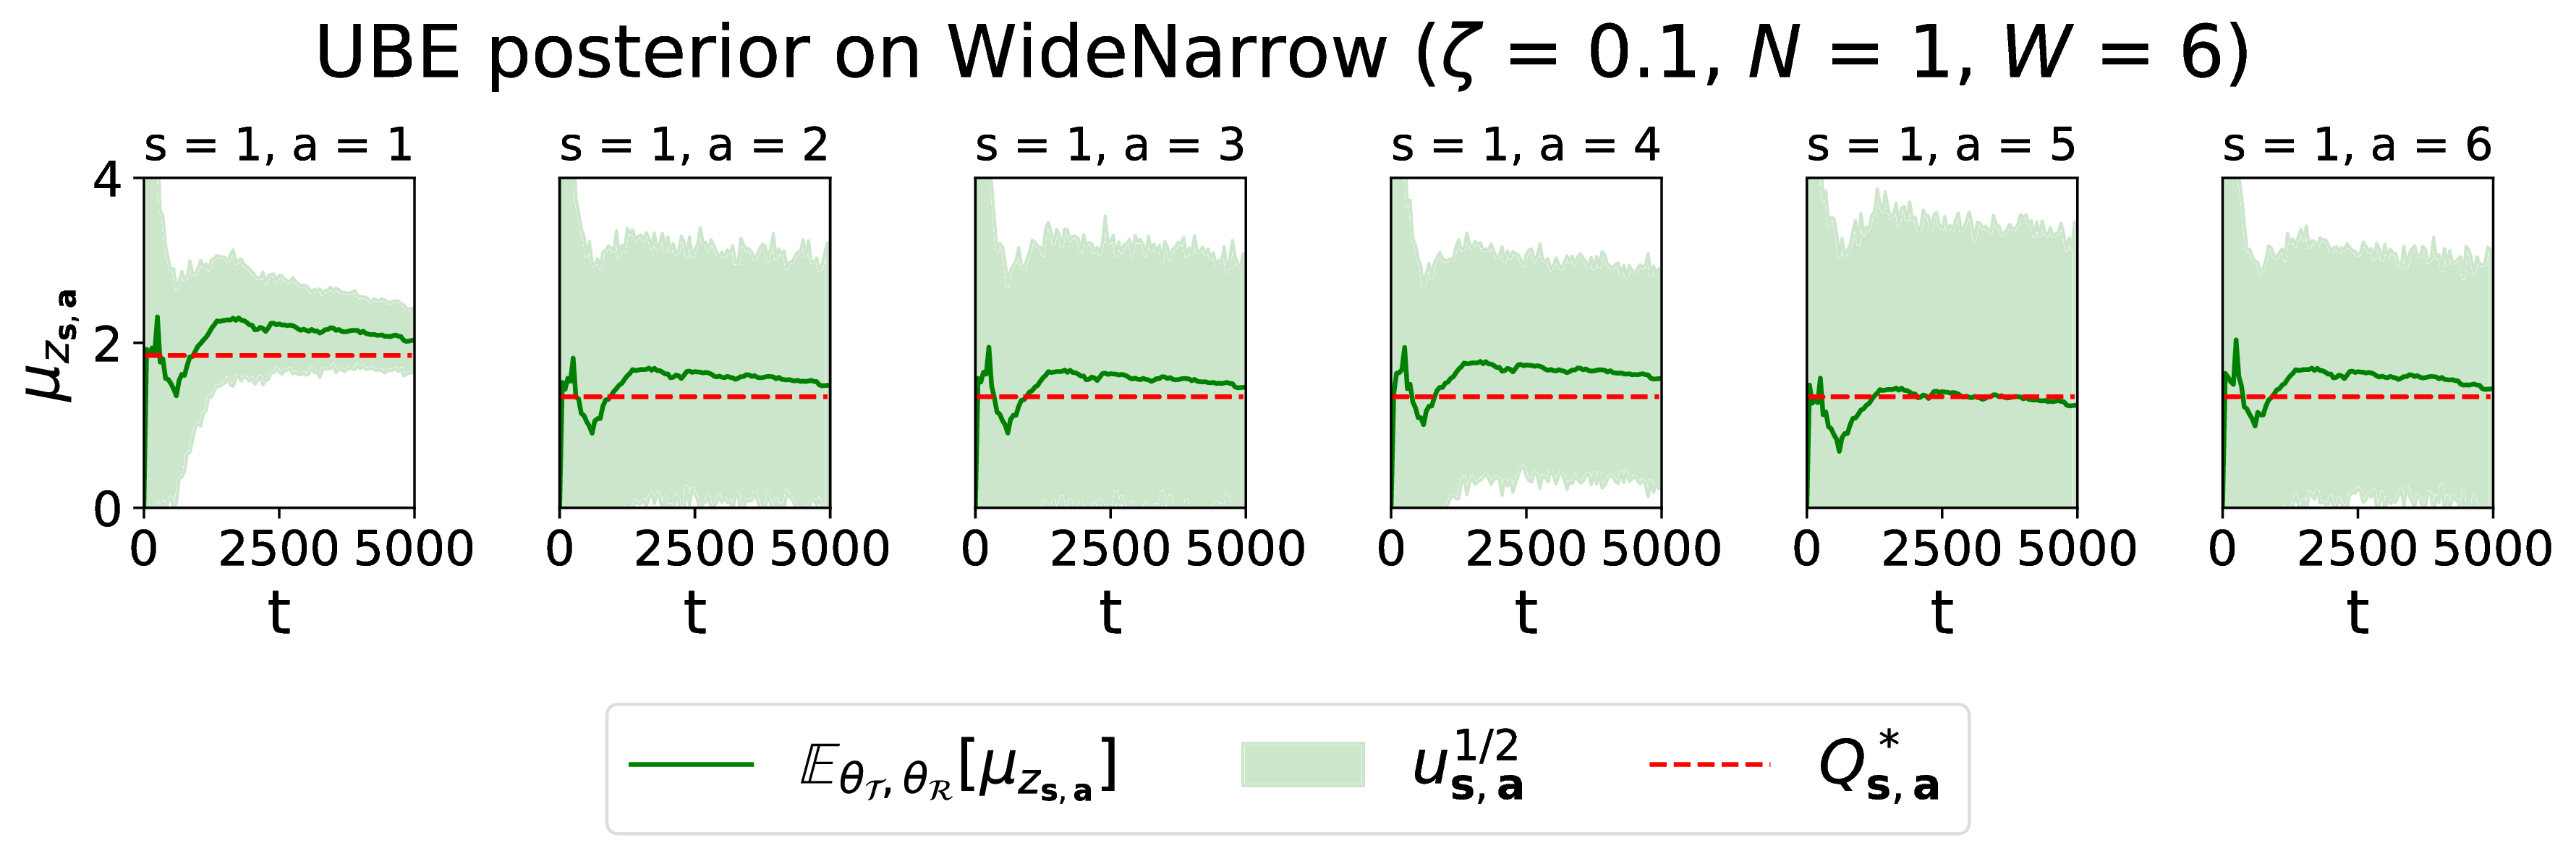
\includegraphics[width=\linewidth]{img/ube-0_0-4_0-3_0-3_0-0_1-posterior-widenarrow-1-6.pdf}
\end{subfigure}
\begin{subfigure}{0.34\textwidth}
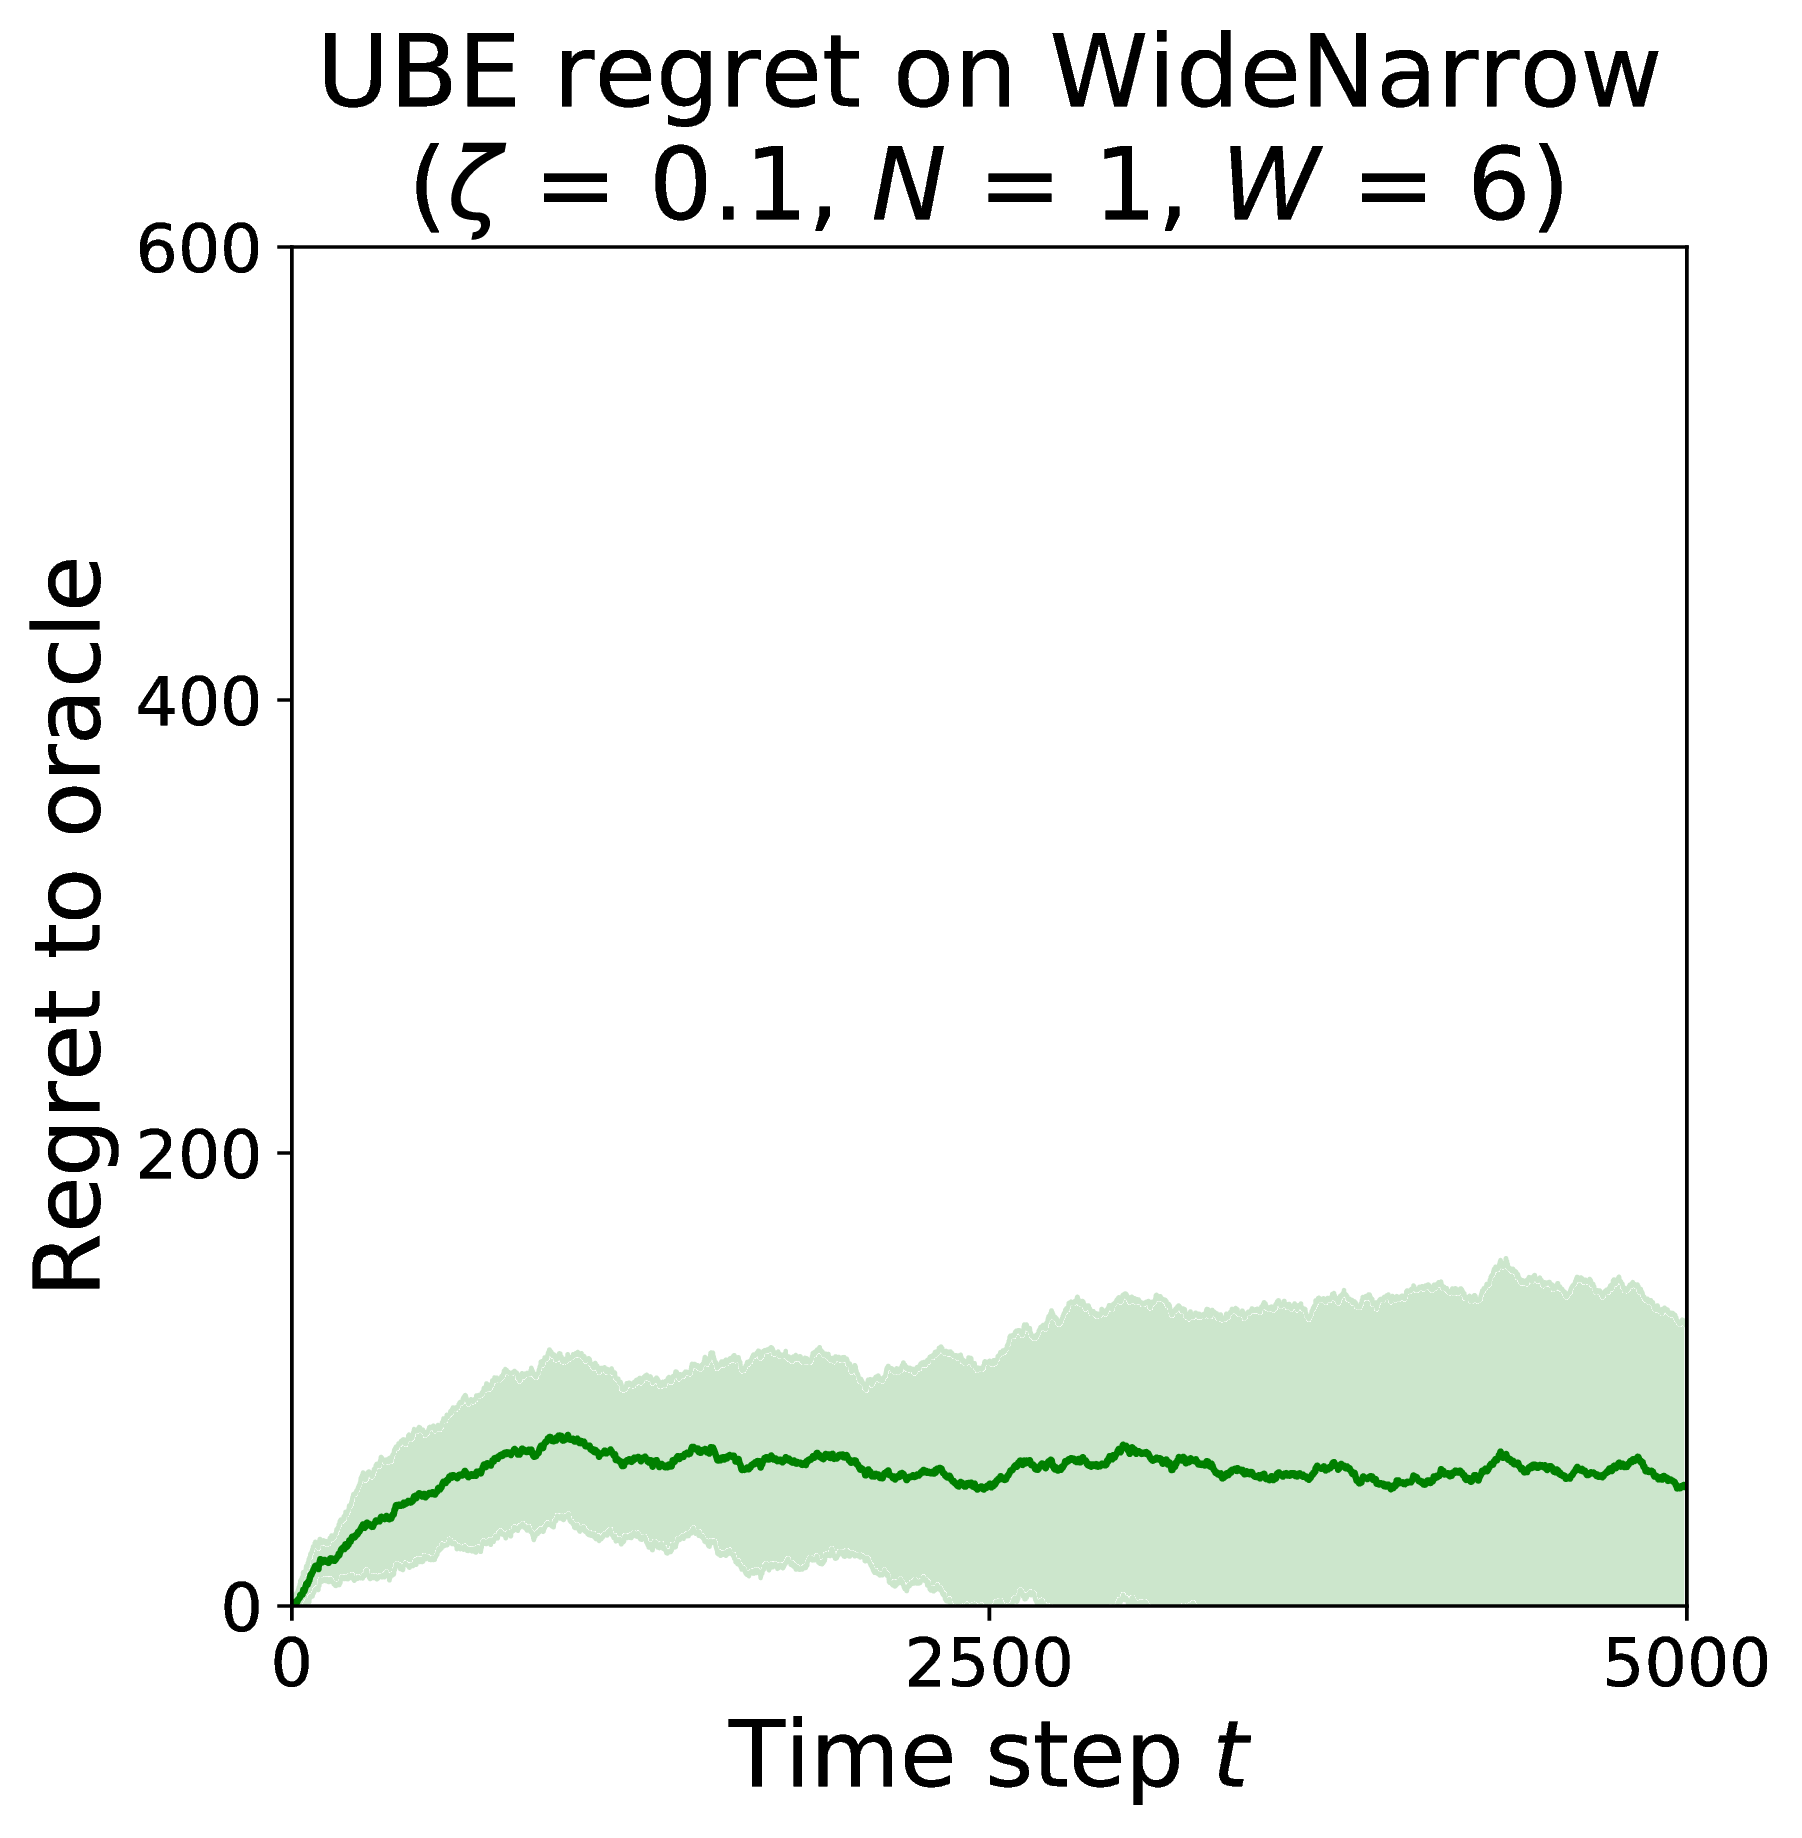
\includegraphics[width=\linewidth]{img/ube-0_0-4_0-3_0-3_0-0_1-regret-widenarrow-1-6.pdf}~\\~\\
\end{subfigure}
\captionsetup{width=0.9\linewidth}
\caption{UBE posterior and regret on WideNarrow.}\label{ube_widenarrow_visual01}
\end{figure}

\begin{figure}[h!]
\centering
\begin{subfigure}{0.65\textwidth}
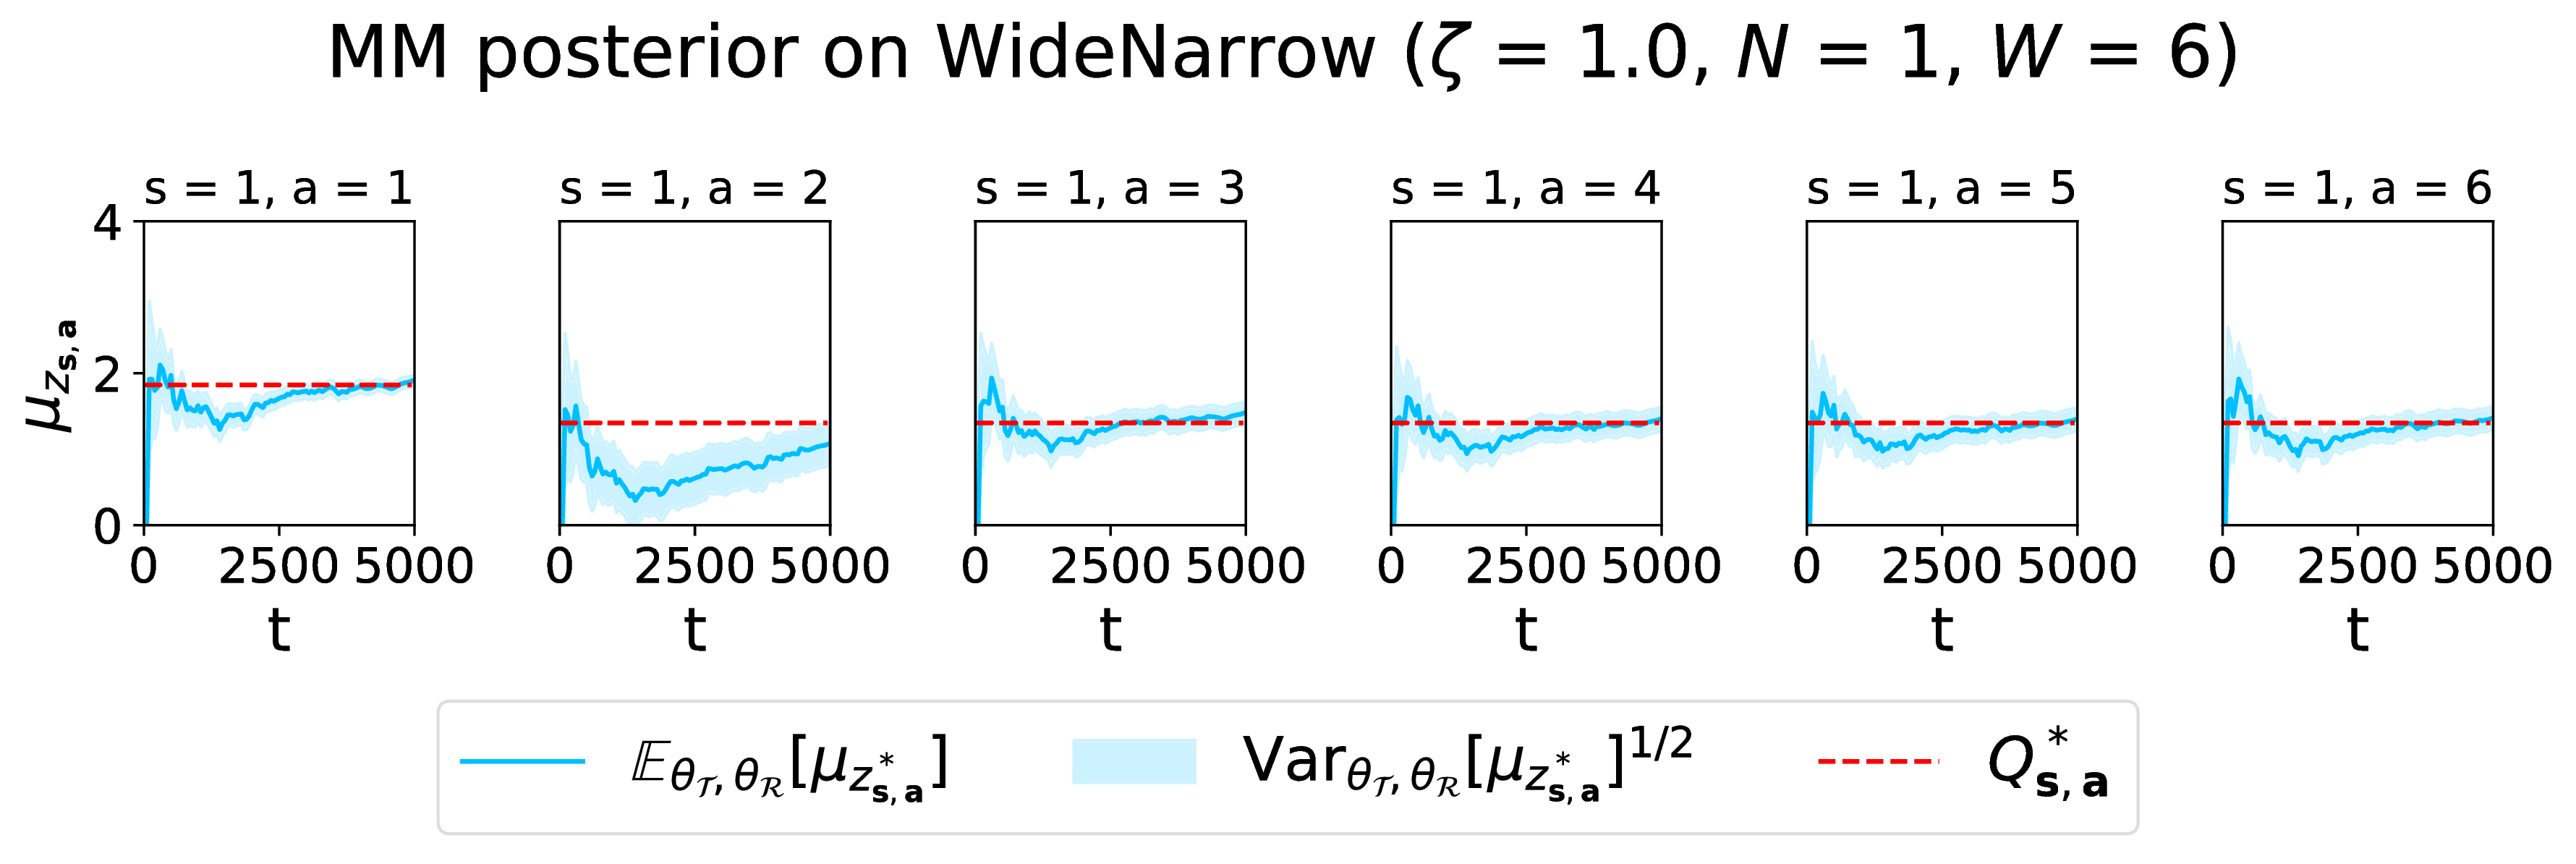
\includegraphics[width=\linewidth]{img/mm-0_0-4_0-3_0-3_0-1_0-posterior-widenarrow-1-6.pdf}
\end{subfigure}
\begin{subfigure}{0.34\textwidth}
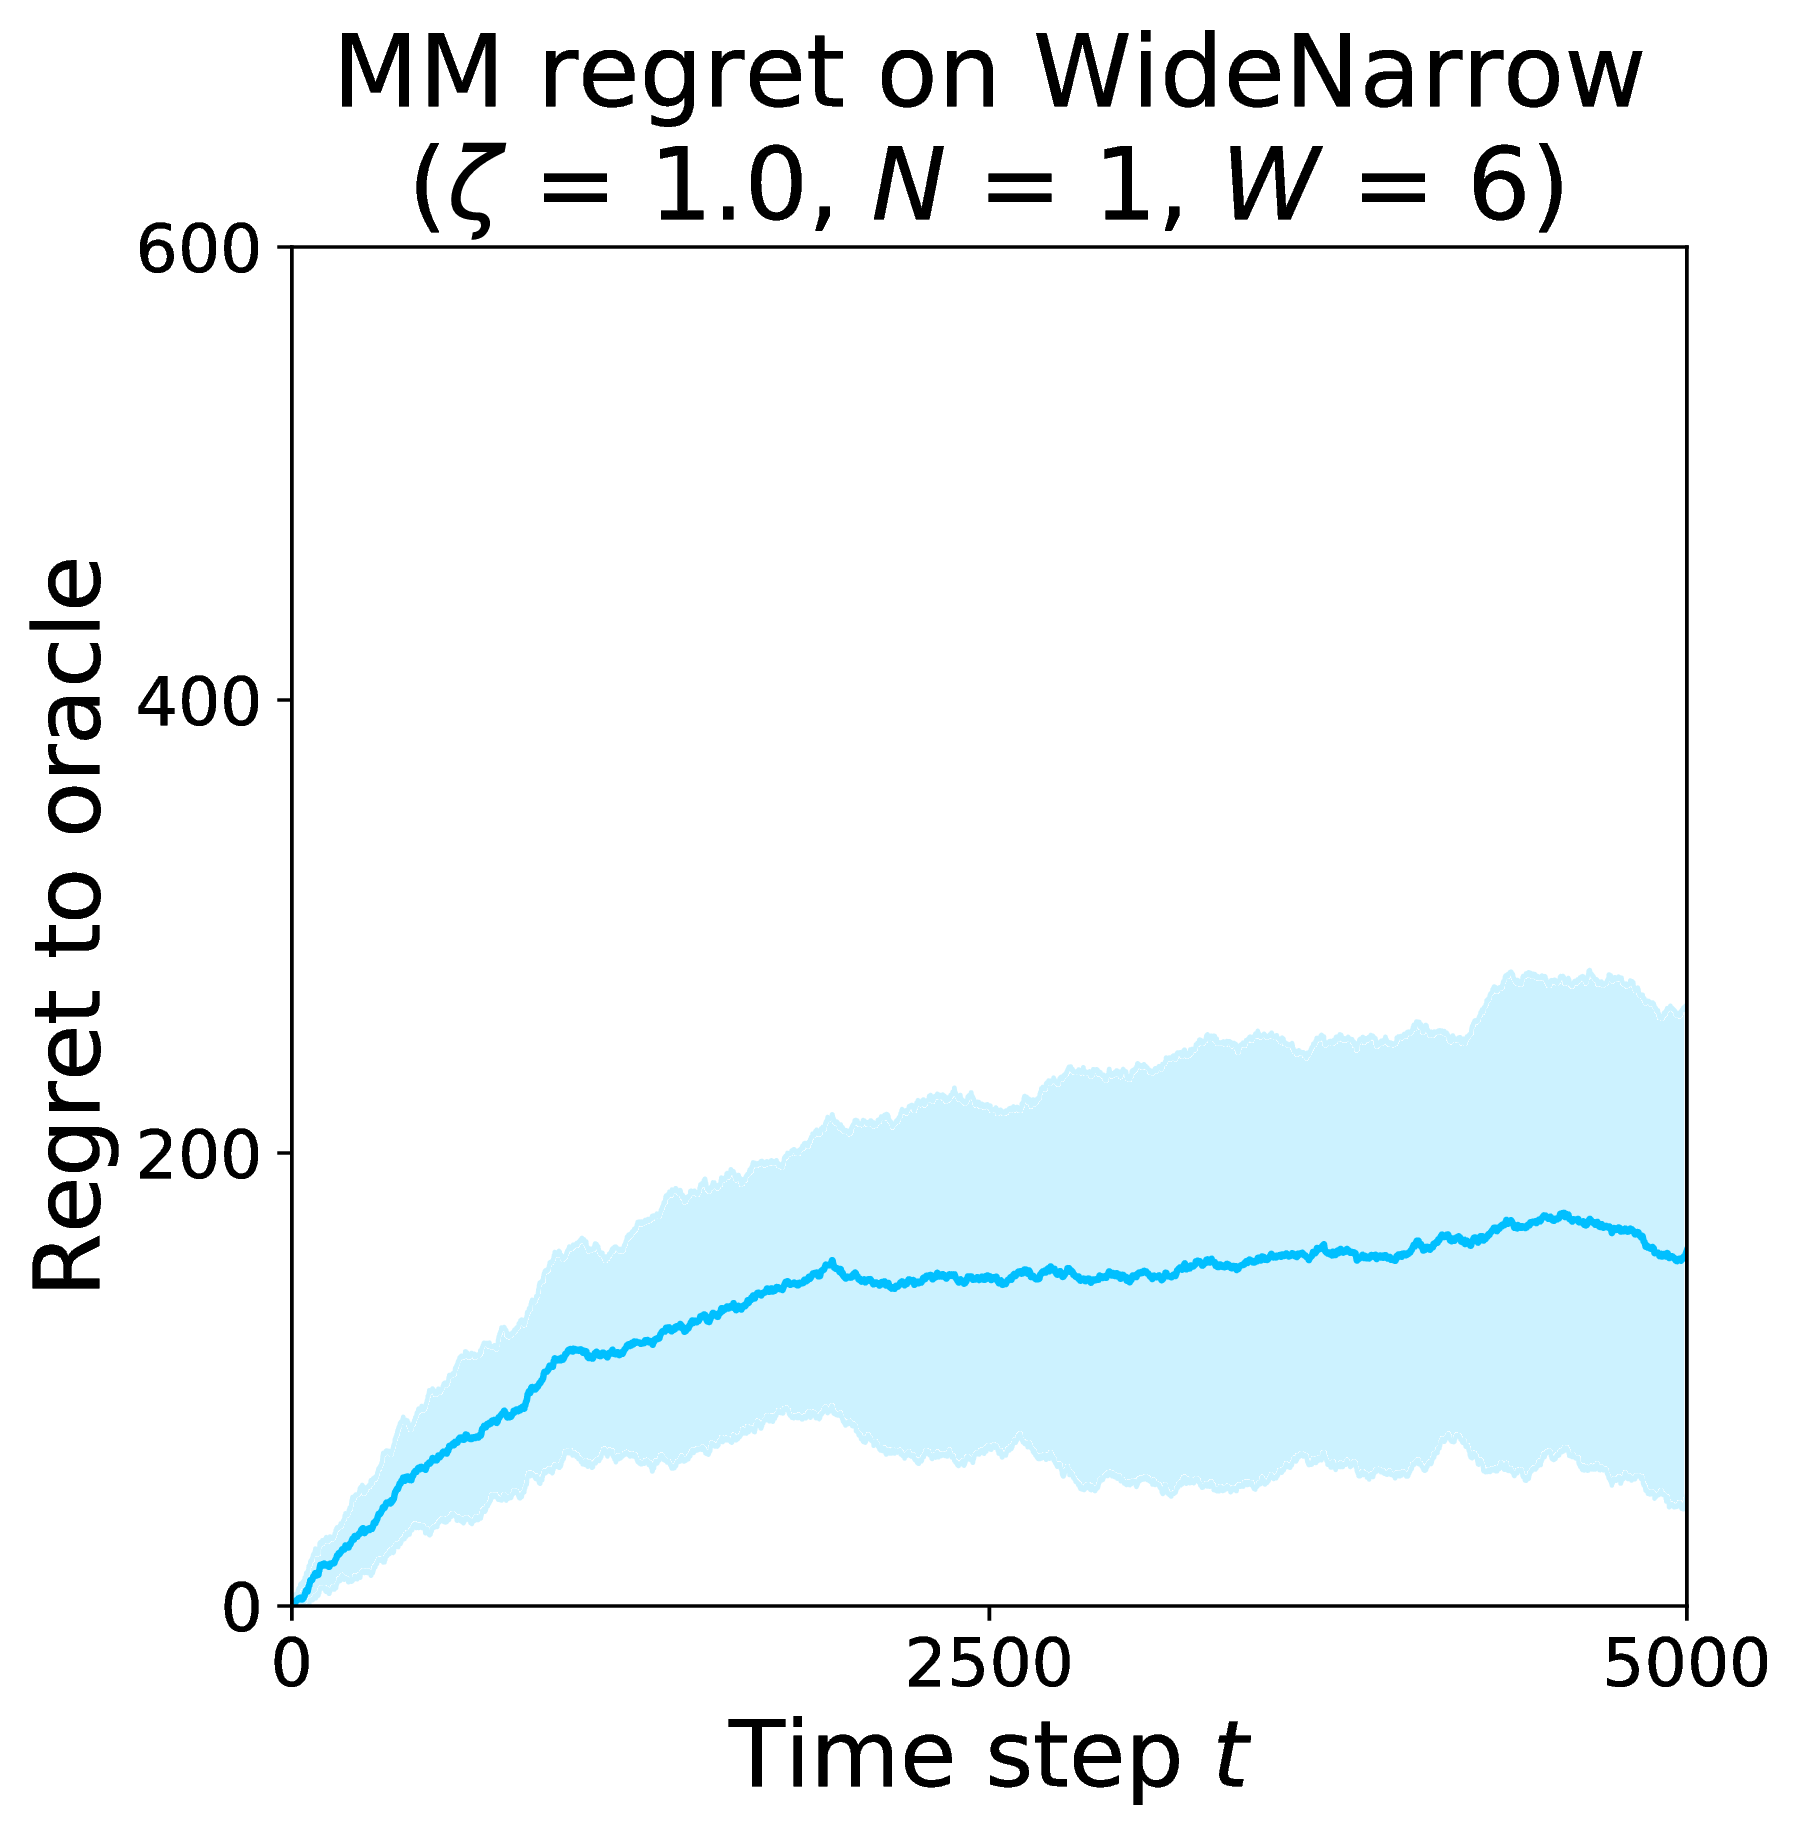
\includegraphics[width=\linewidth]{img/mm-0_0-4_0-3_0-3_0-1_0-regret-widenarrow-1-6.pdf}~\\~\\
\end{subfigure}
\captionsetup{width=0.9\linewidth}
\caption{MM posterior and regret on WideNarrow.}\label{mm_widenarrow_visual}
\end{figure}

\clearpage

\begin{figure}[h!]
\centering
\begin{subfigure}{1.0\textwidth}
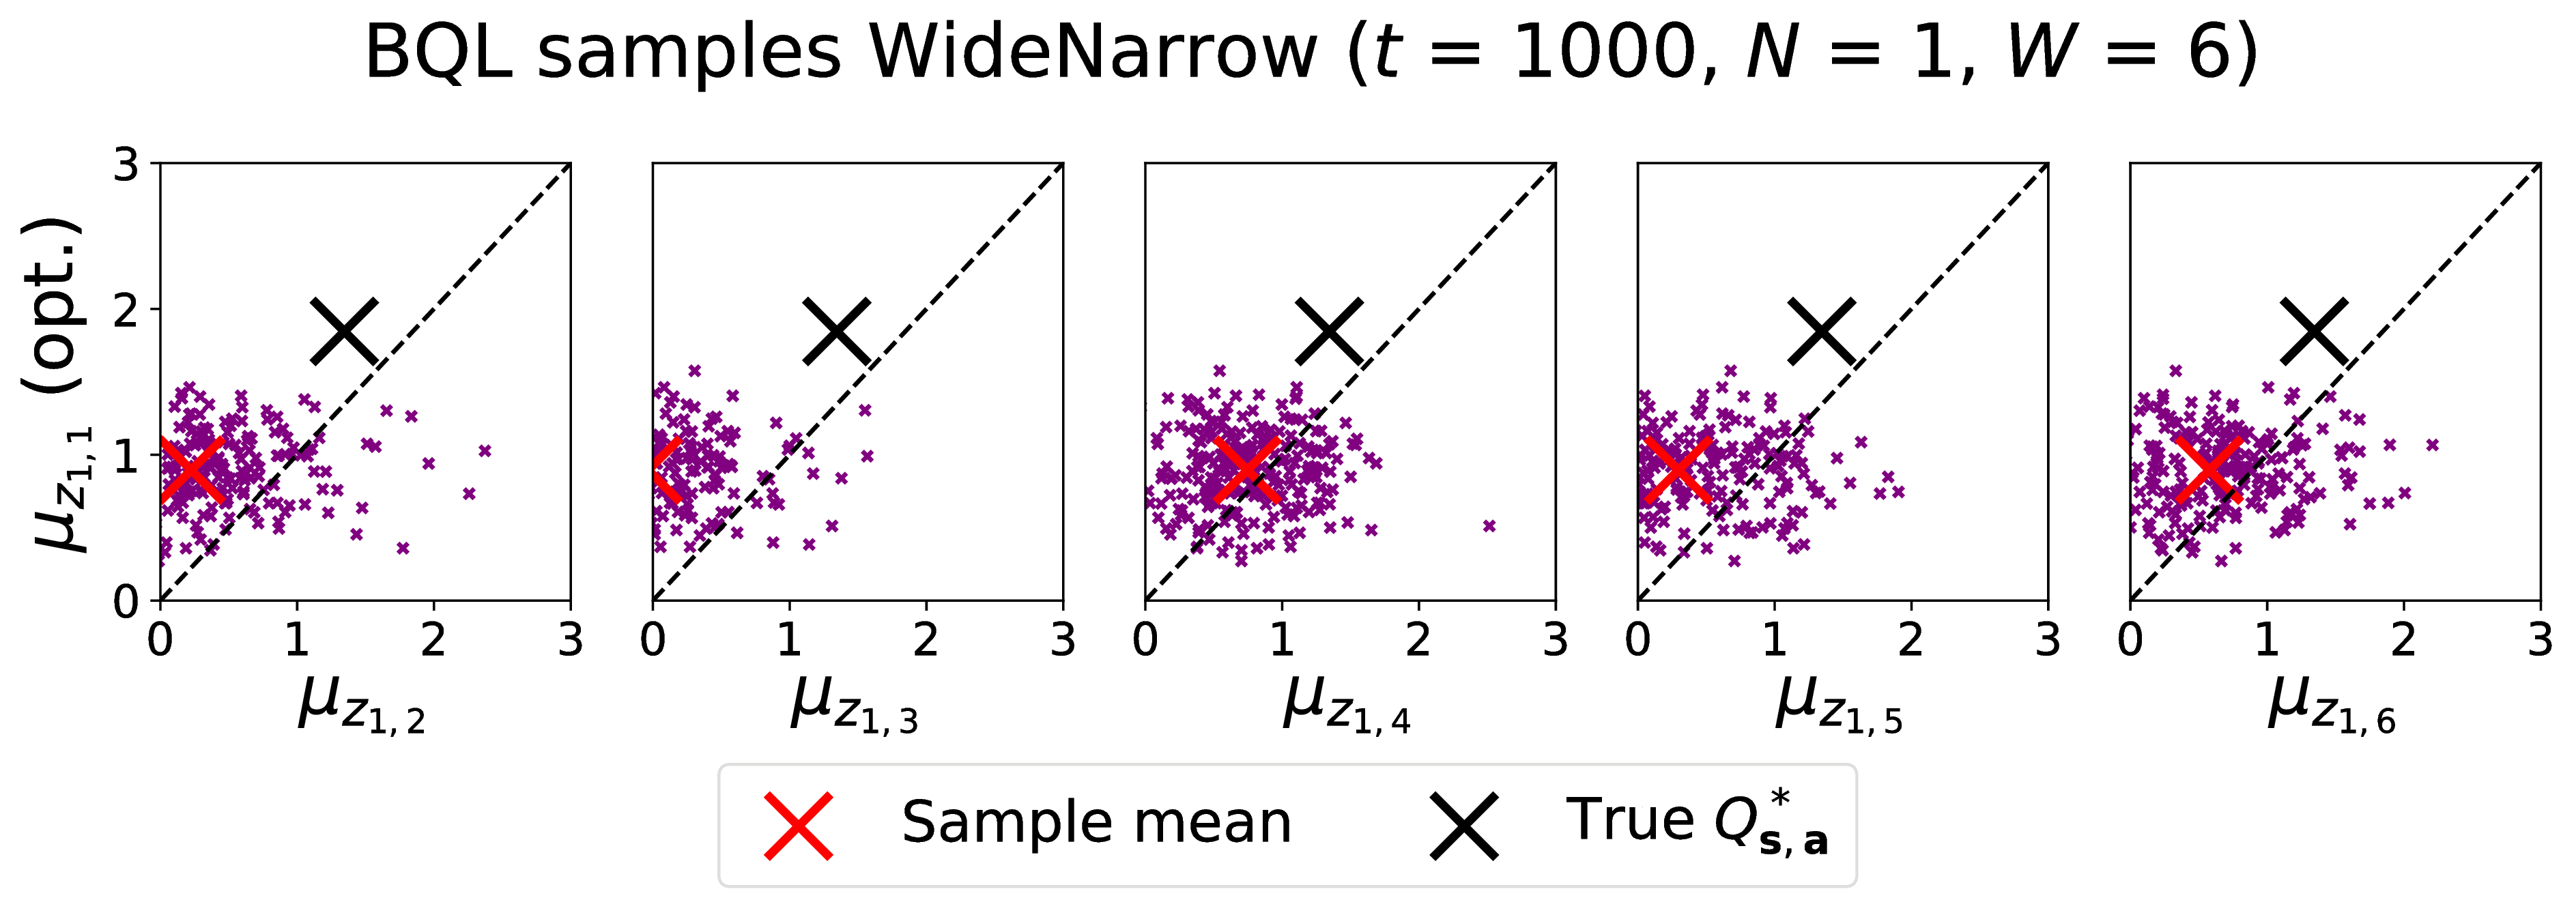
\includegraphics[width=\linewidth]{img/bql-0_0-4_0-3_0-3_0-scatter-widenarrow-1-6-1000.pdf}
\end{subfigure}\\
~\\
~\\
\begin{subfigure}{1.0\textwidth}
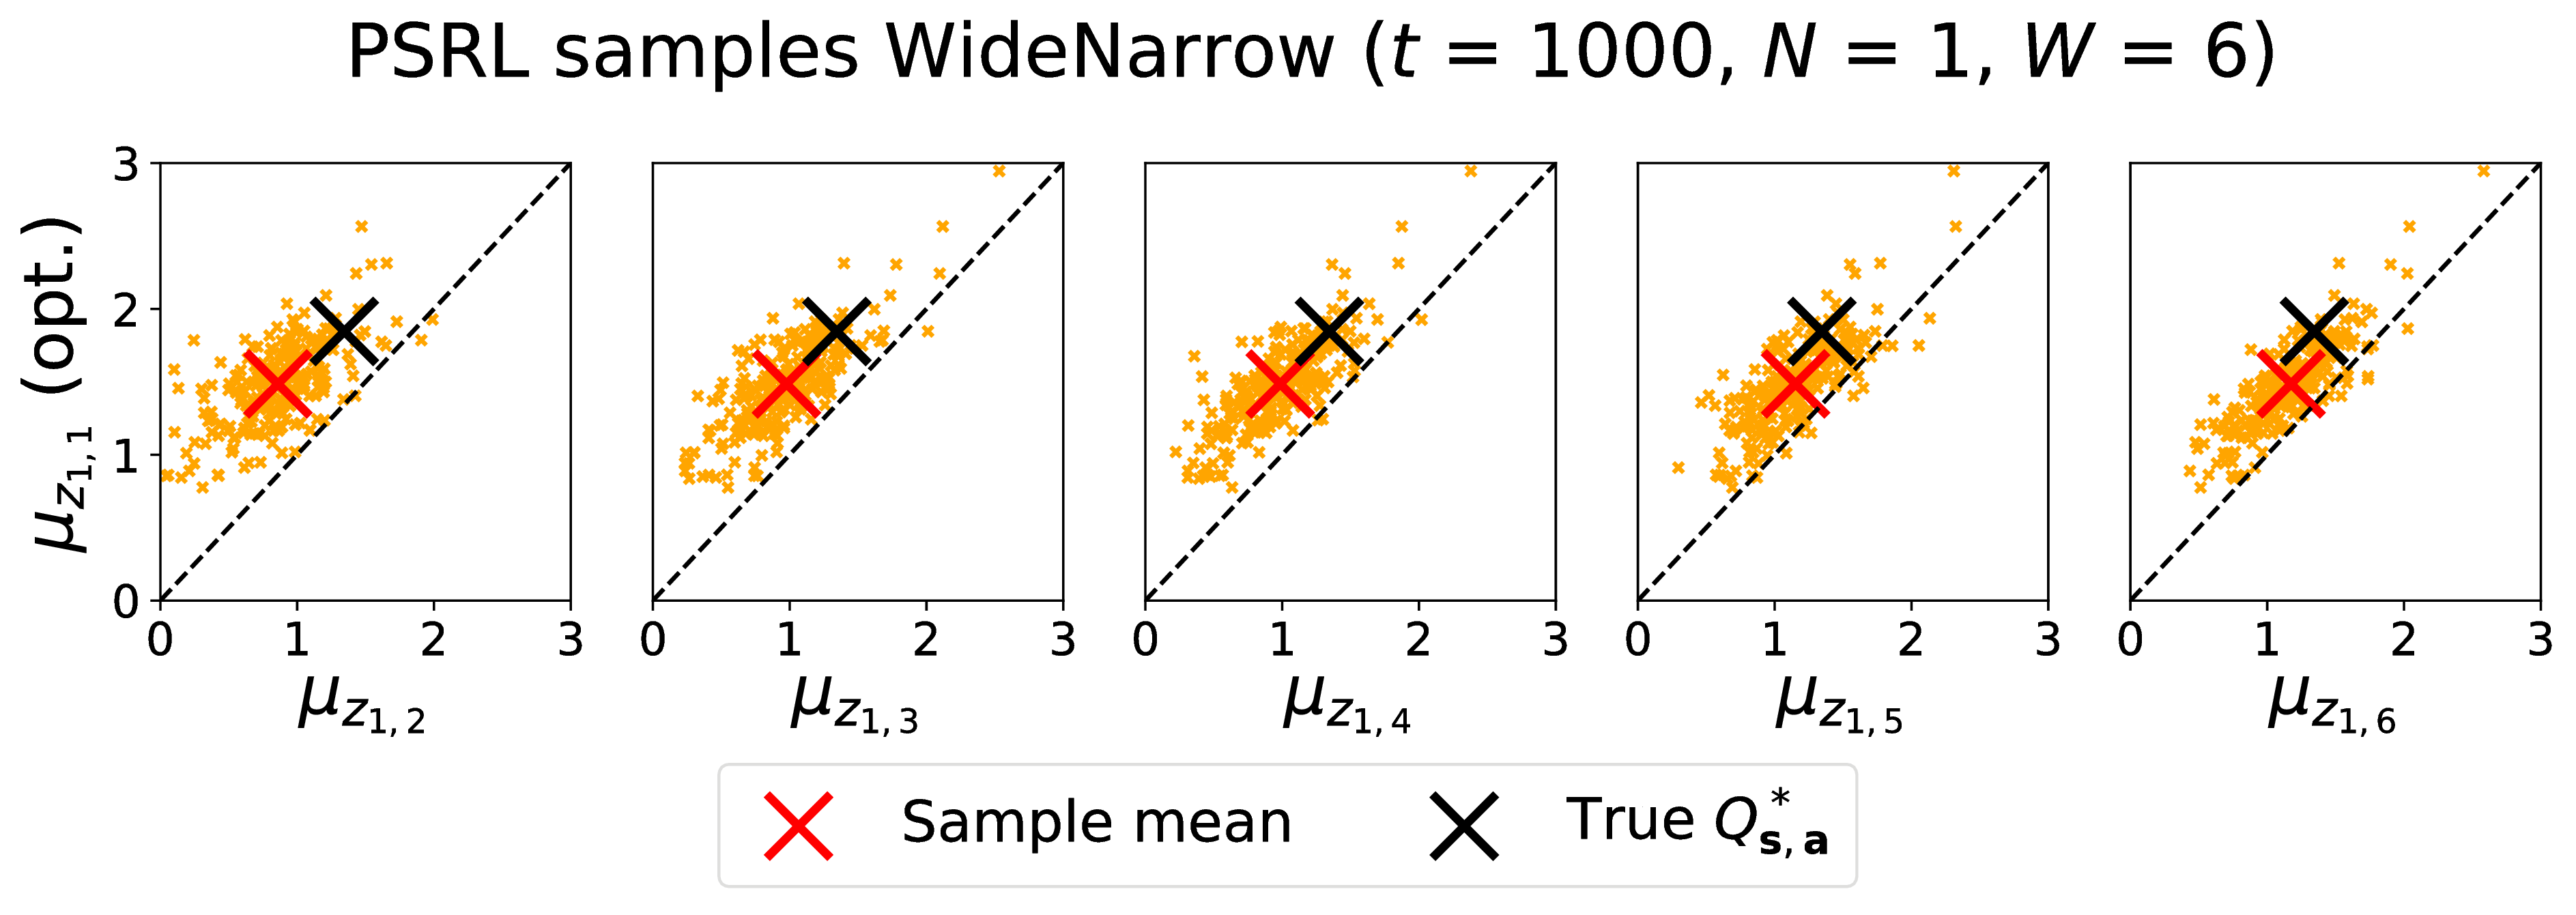
\includegraphics[width=\linewidth]{img/psrl-0_0-4_0-3_0-3_0-scatter-widenarrow-1-6-1000.pdf}
\end{subfigure}\\
~\\
~\\
\begin{subfigure}{1.0\textwidth}
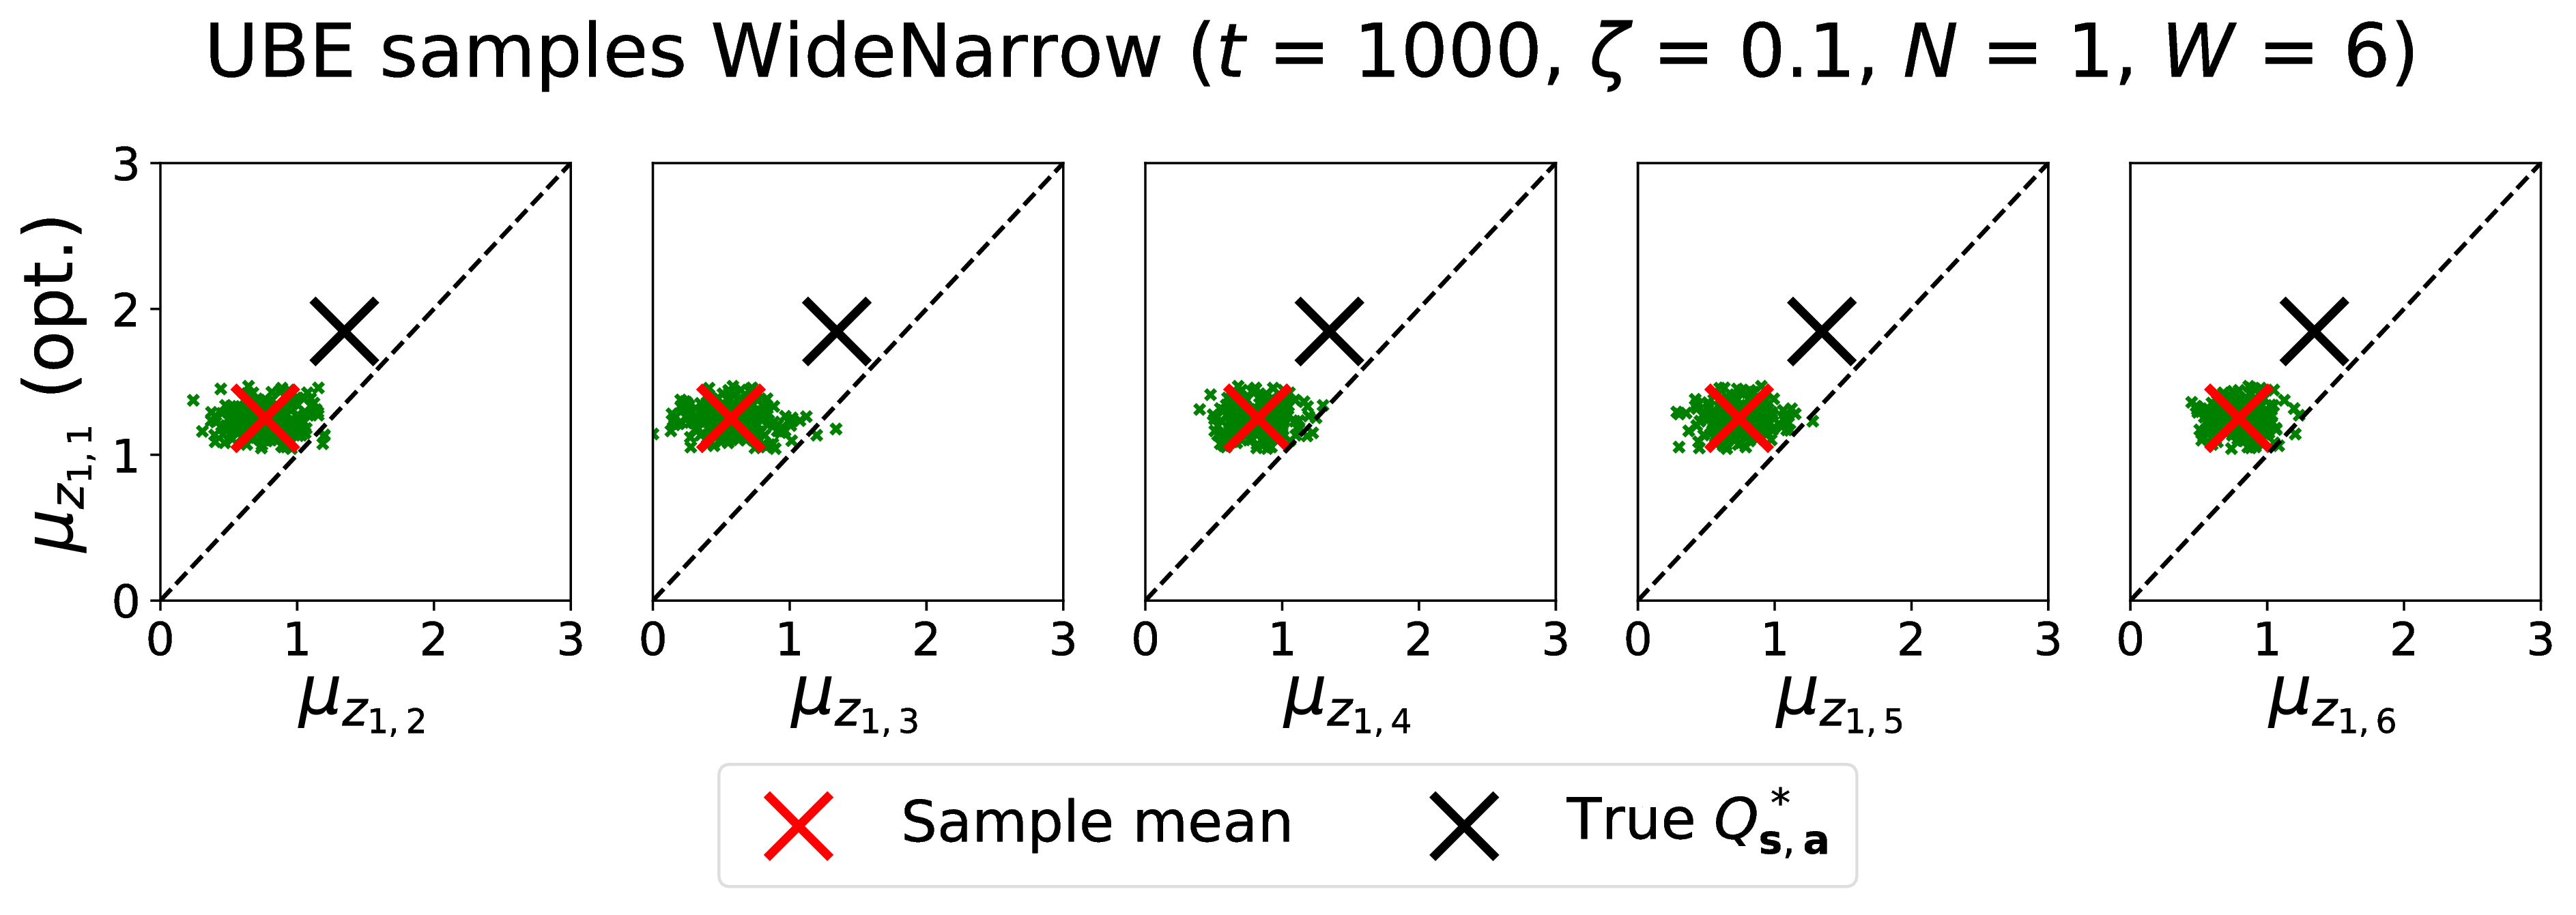
\includegraphics[width=\linewidth]{img/ube-0_0-4_0-3_0-3_0-0_1-scatter-widenarrow-1-6-1000.pdf}
\end{subfigure}\\
~\\
~\\
\begin{subfigure}{1.0\textwidth}
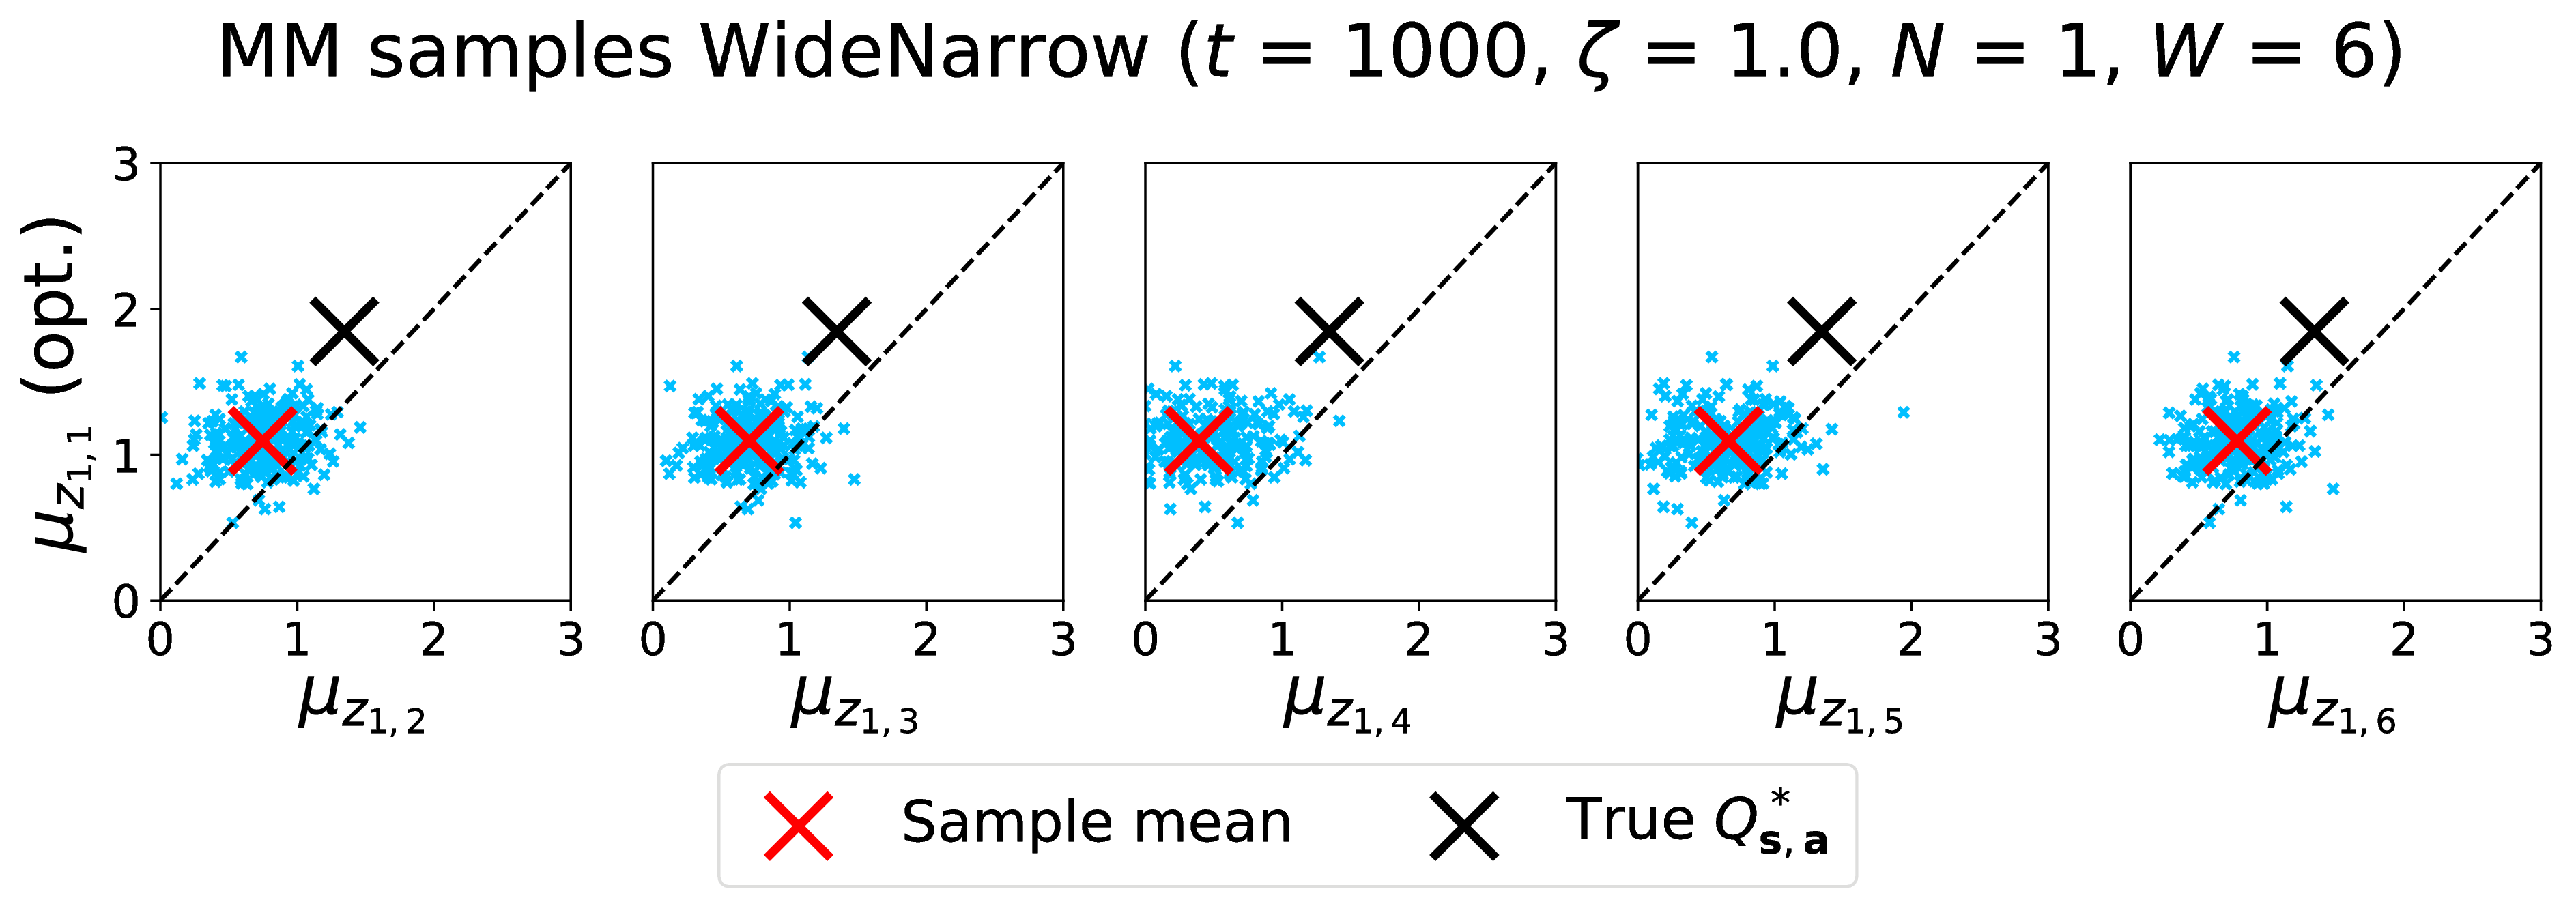
\includegraphics[width=\linewidth]{img/mm-0_0-4_0-3_0-3_0-1_0-scatter-widenarrow-1-6-1000.pdf}
\end{subfigure}\\
\captionsetup{width=0.9\linewidth}
\caption{Correlation plots for WideNarrow at time step $t = 1,000$.}\label{correlations_widenarrow_500}
\end{figure}

\begin{figure}[h!]
\centering
\begin{subfigure}{1.0\textwidth}
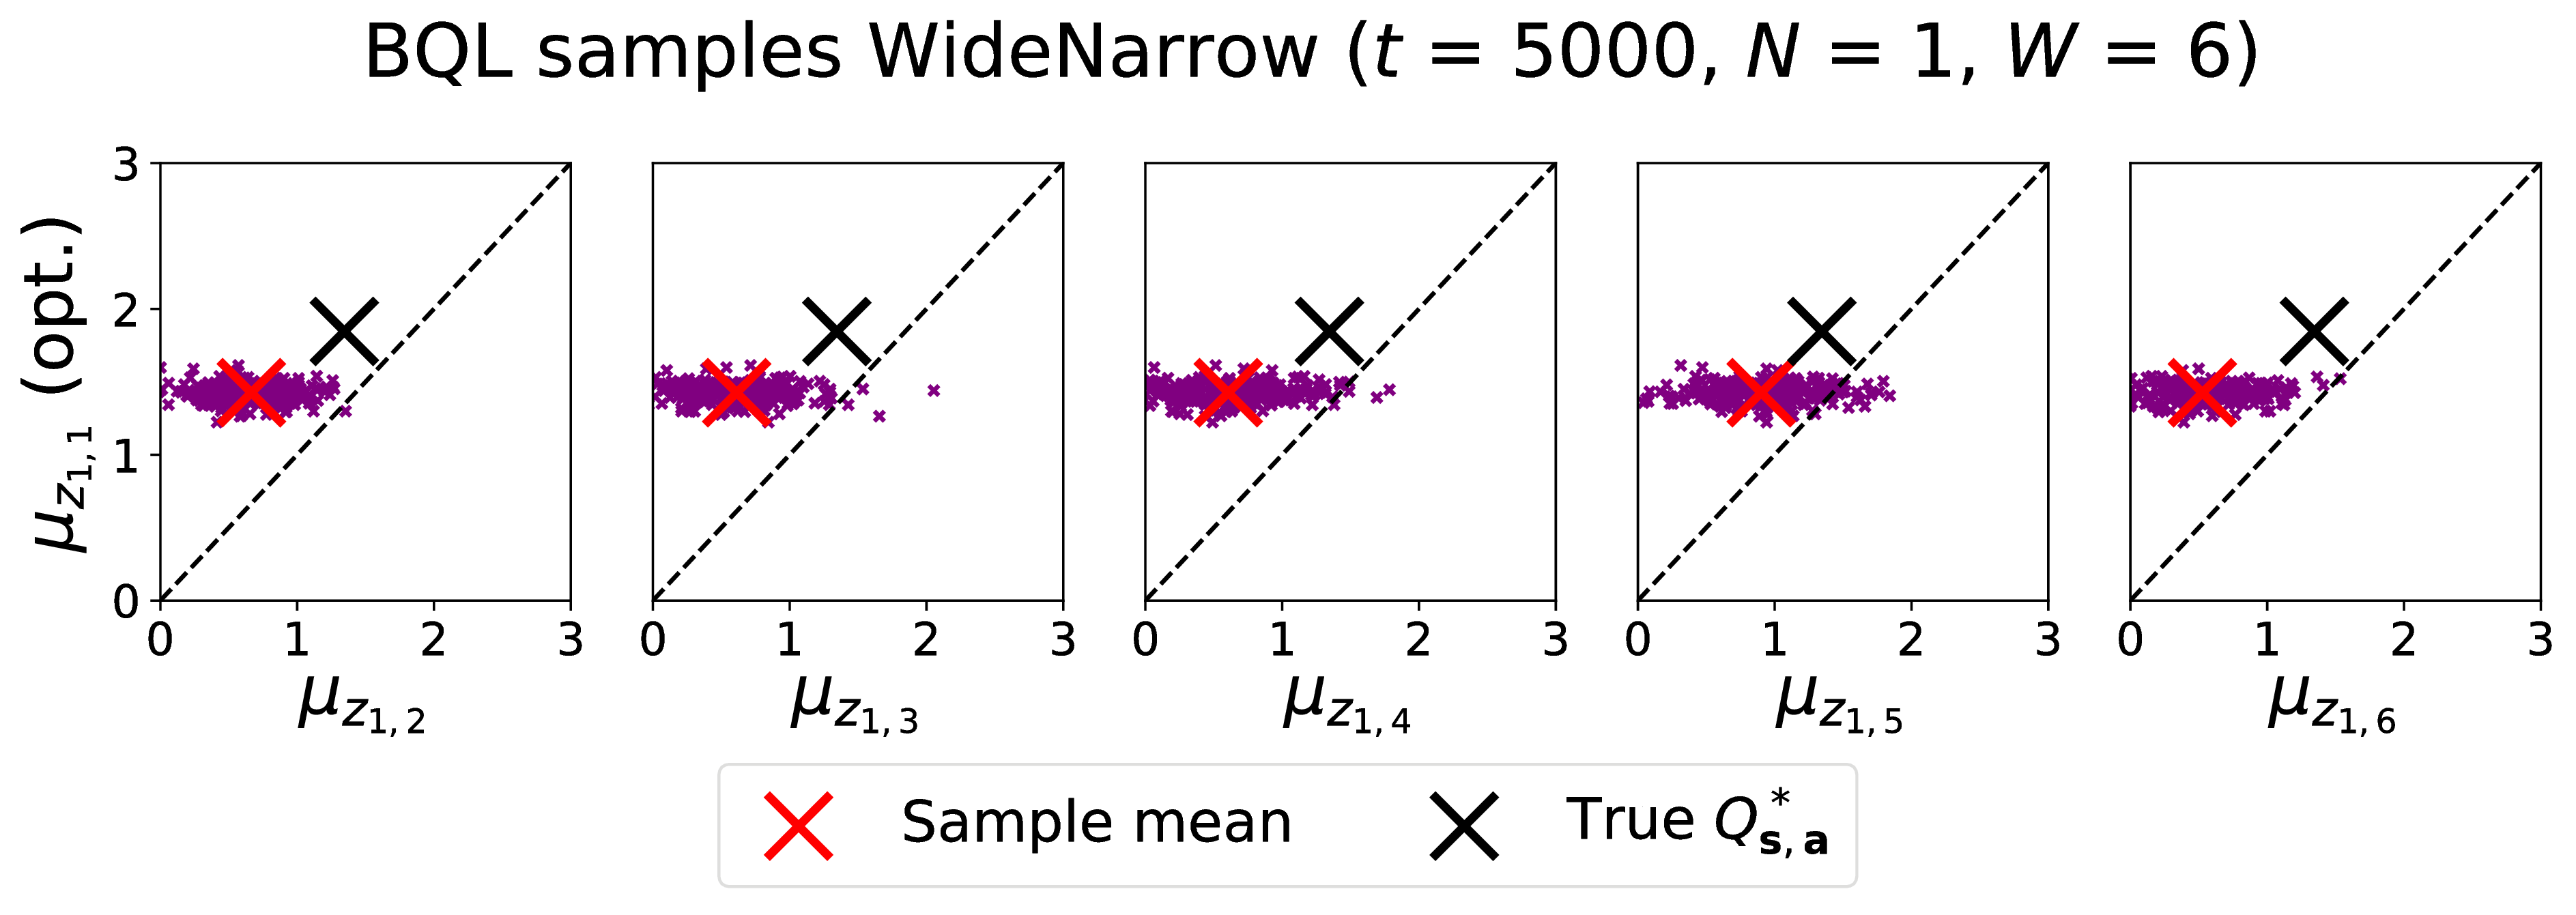
\includegraphics[width=\linewidth]{img/bql-0_0-4_0-3_0-3_0-scatter-widenarrow-1-6-5000.pdf}
\end{subfigure}\\
~\\
~\\
\begin{subfigure}{1.0\textwidth}
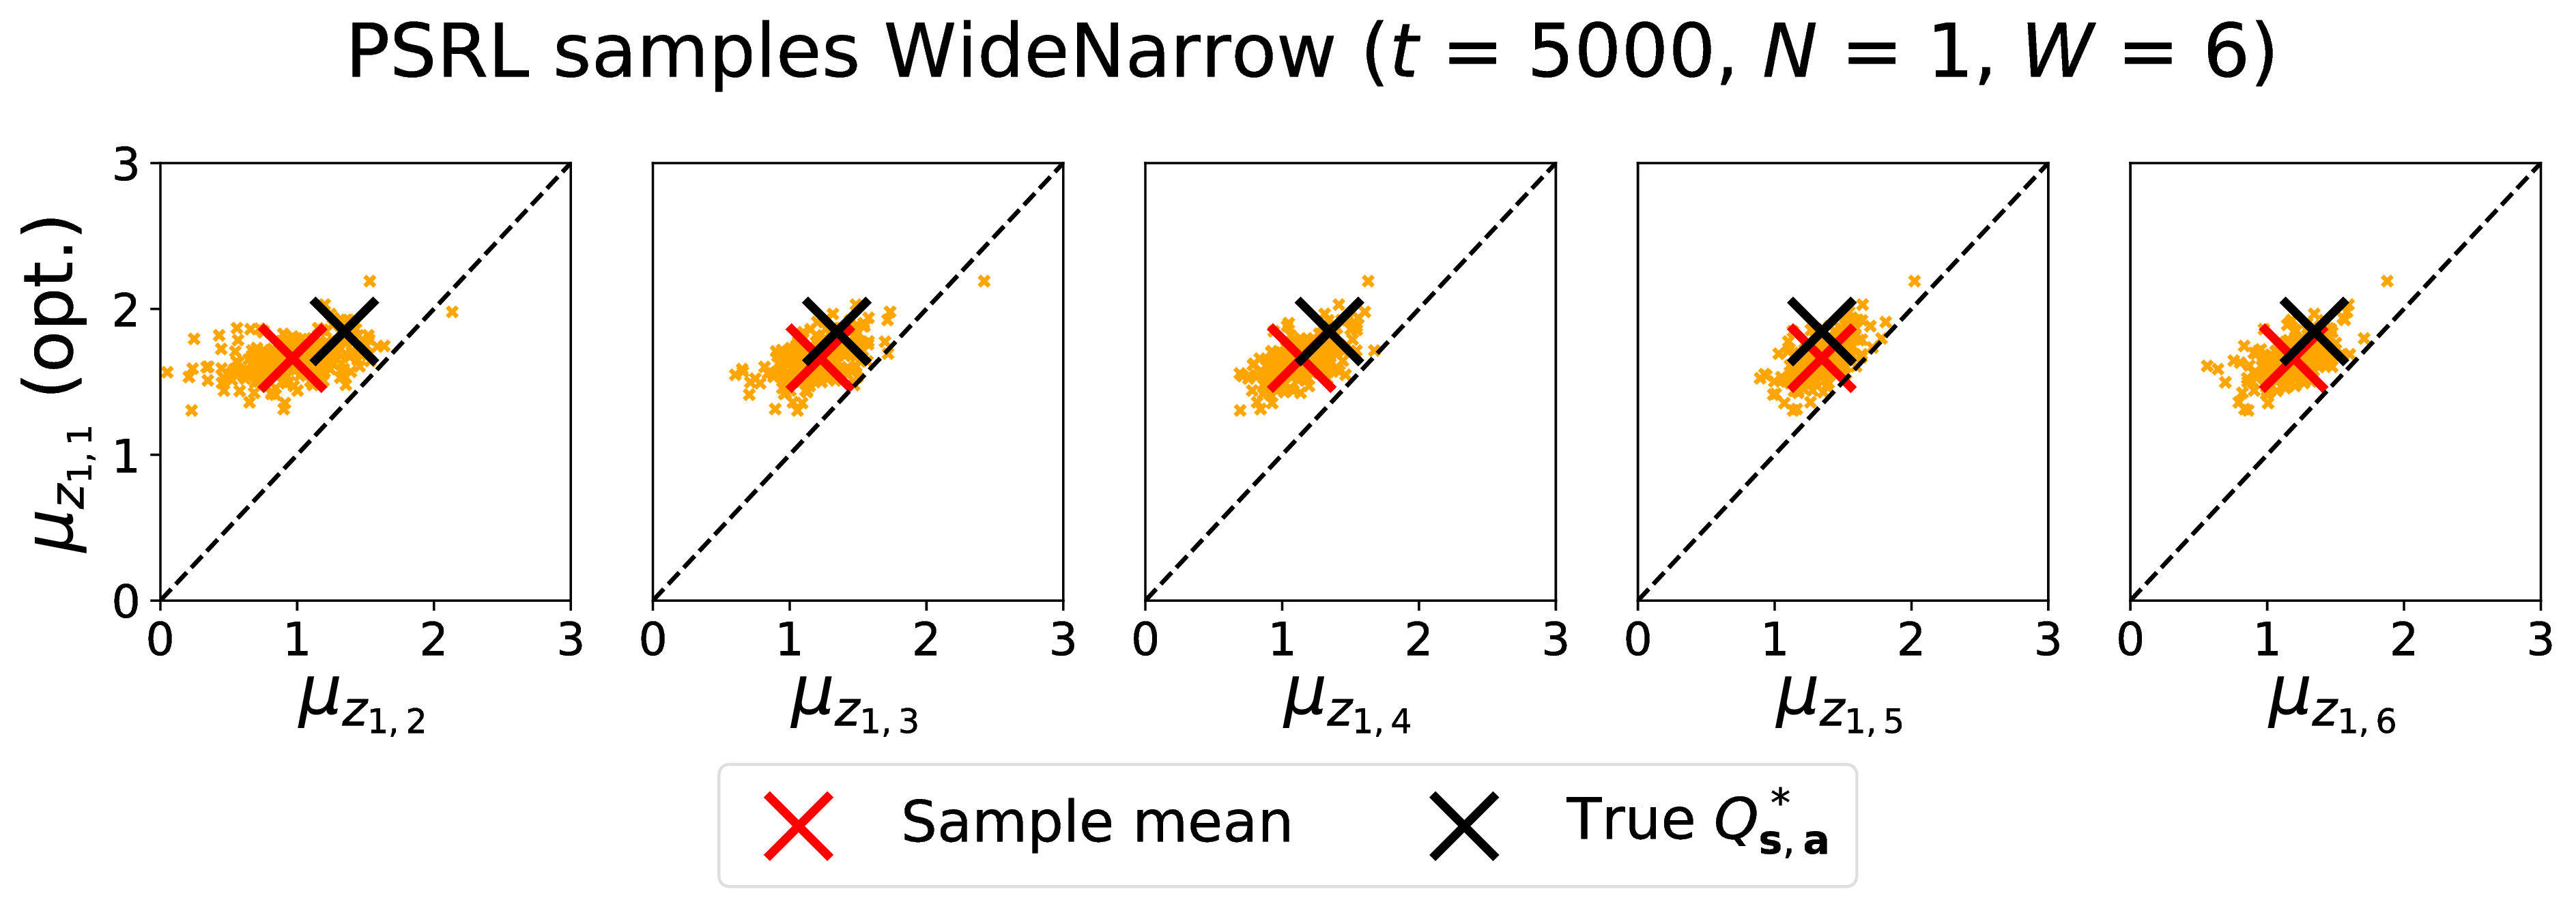
\includegraphics[width=\linewidth]{img/psrl-0_0-4_0-3_0-3_0-scatter-widenarrow-1-6-5000.pdf}
\end{subfigure}\\
~\\
~\\
\begin{subfigure}{1.0\textwidth}
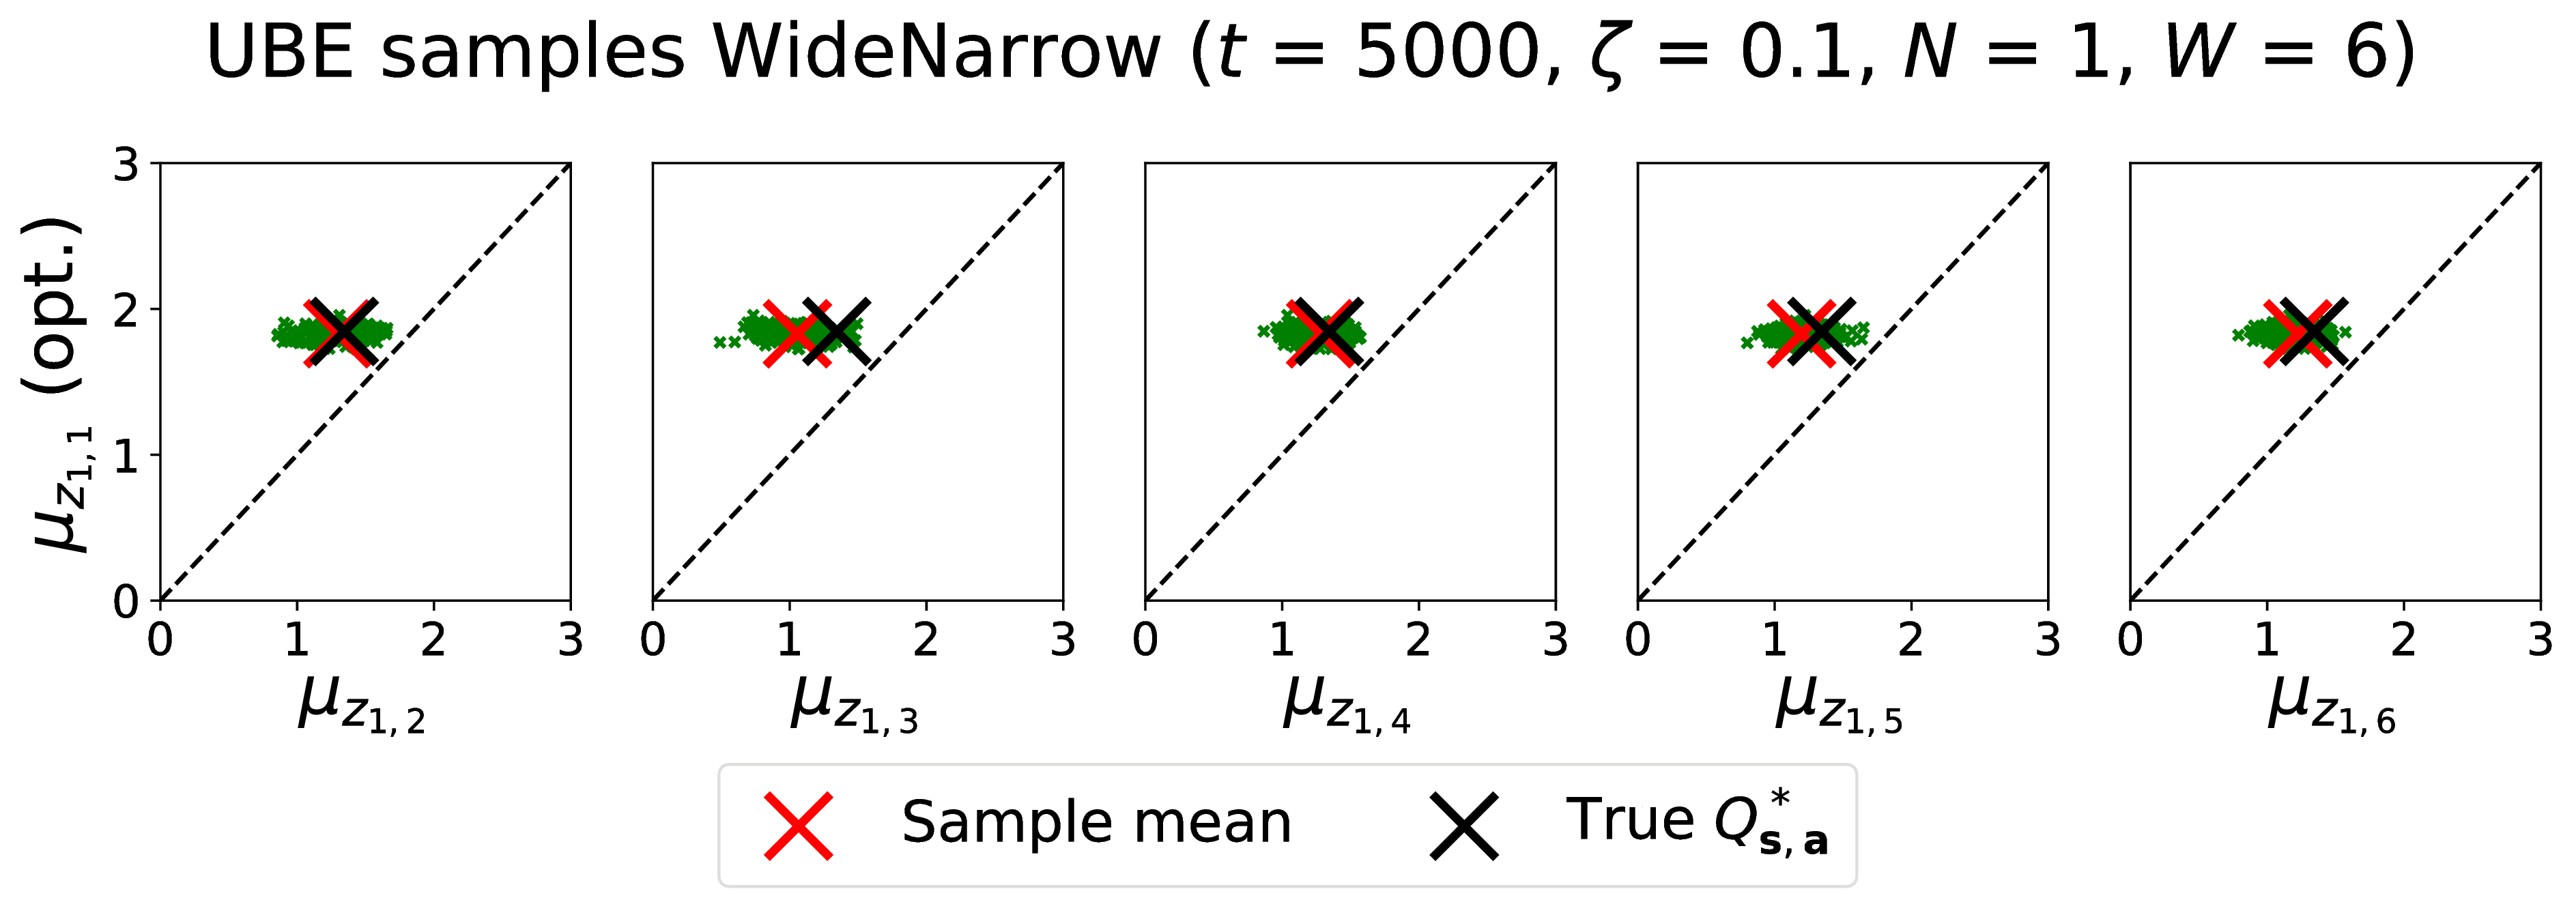
\includegraphics[width=\linewidth]{img/ube-0_0-4_0-3_0-3_0-0_1-scatter-widenarrow-1-6-5000.pdf}
\end{subfigure}\\
~\\
~\\
\begin{subfigure}{1.0\textwidth}
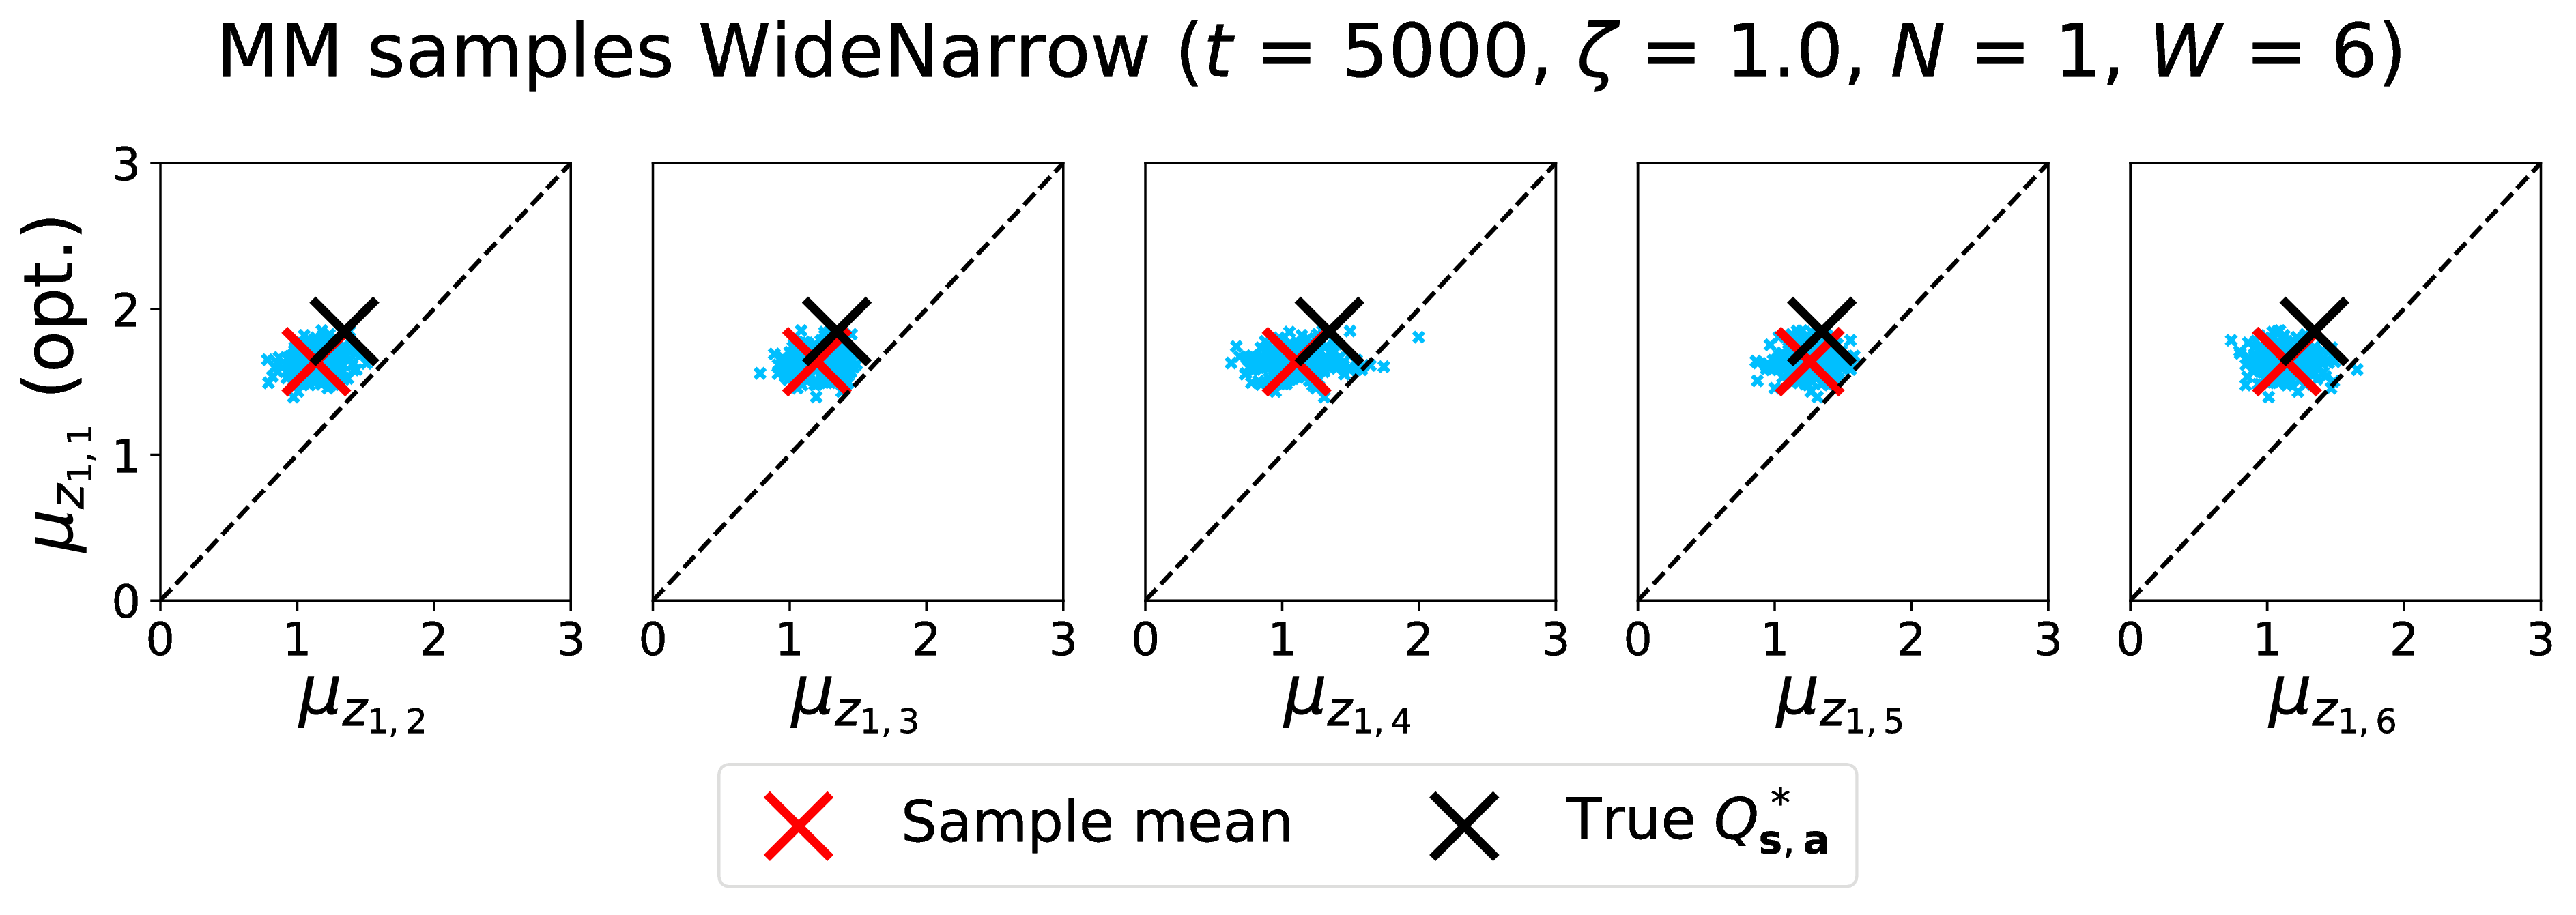
\includegraphics[width=\linewidth]{img/mm-0_0-4_0-3_0-3_0-1_0-scatter-widenarrow-1-6-5000.pdf}
\end{subfigure}\\
\captionsetup{width=0.9\linewidth}
\caption{Correlation plots for WideNarrow at time step $t = 5,000$.}\label{correlations_widenarrow_2500}
\end{figure}

% ============================================================
% PriorMDP
% ============================================================

\clearpage

\subsection{PriorMDP}

\begin{figure}[h!]
\centering
\begin{subfigure}{0.65\textwidth}
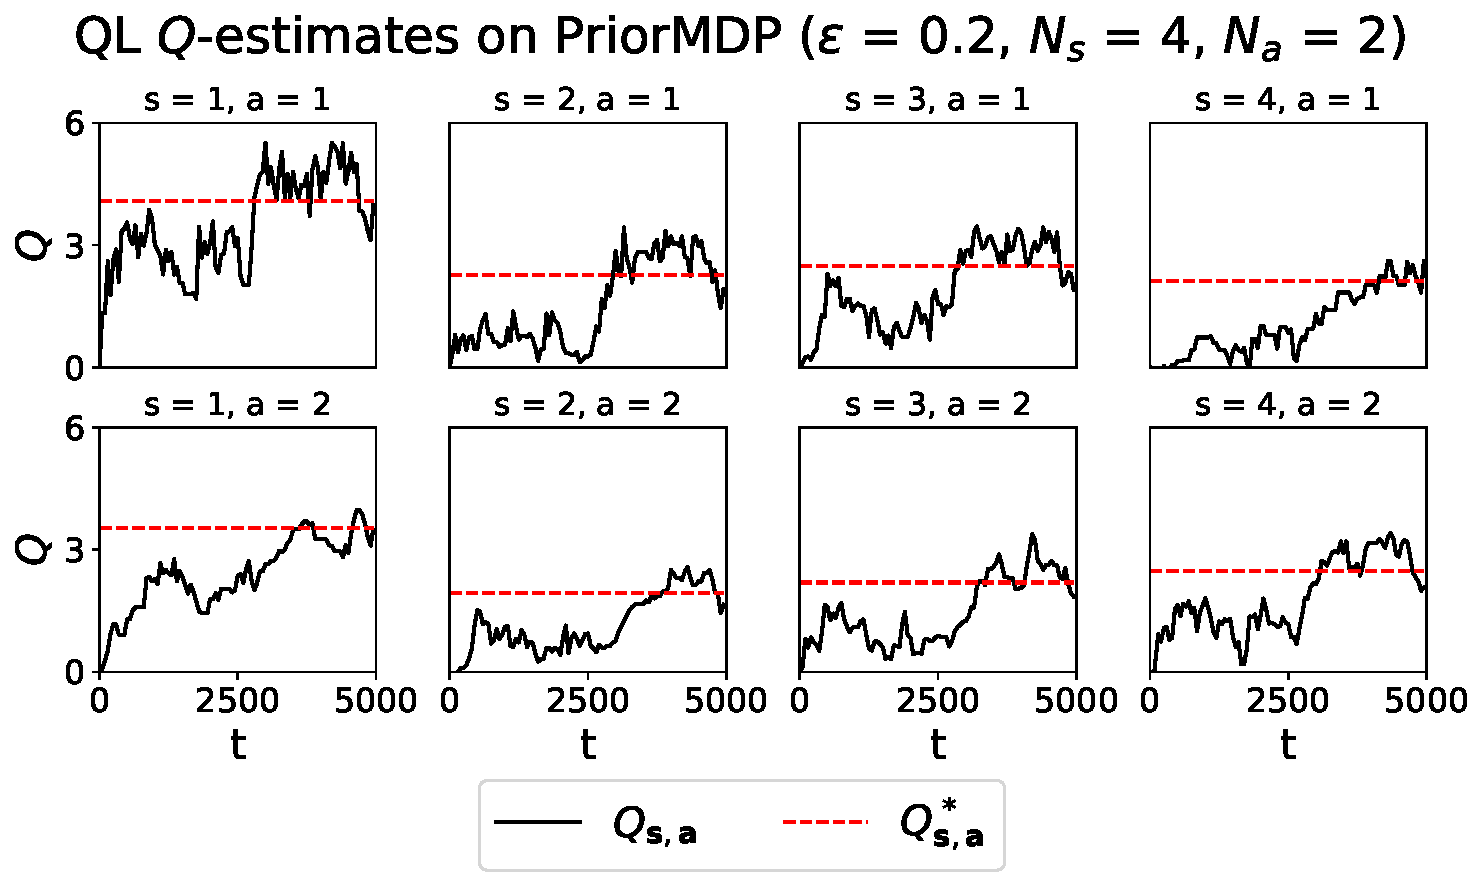
\includegraphics[width=\linewidth]{img/ql-0_2-qestimates-priormdp-4-2.pdf}
\end{subfigure}
\begin{subfigure}{0.34\textwidth}
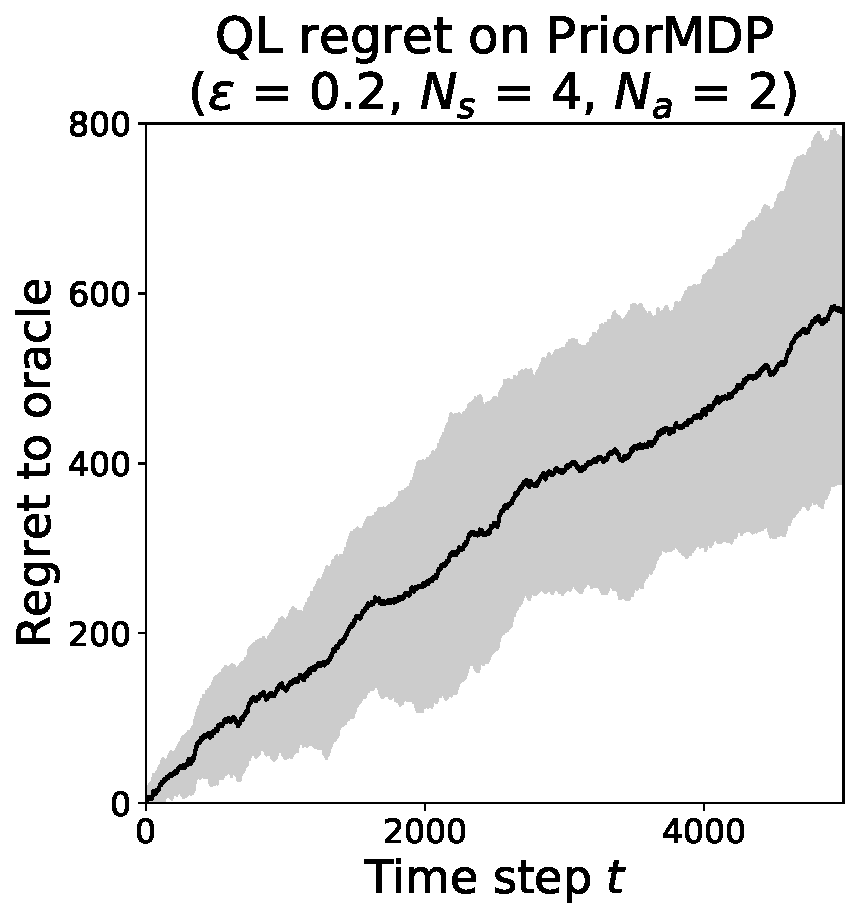
\includegraphics[width=\linewidth]{img/ql-0_2-regret-priormdp-4-2.pdf}~\\~\\
\end{subfigure}
\captionsetup{width=0.9\linewidth}
\caption{QL $Q$-estimates and regret on PriorMDP.}\label{ql_priormdp_visual}
\end{figure}


\begin{figure}[h!]
\centering
\begin{subfigure}{0.65\textwidth}
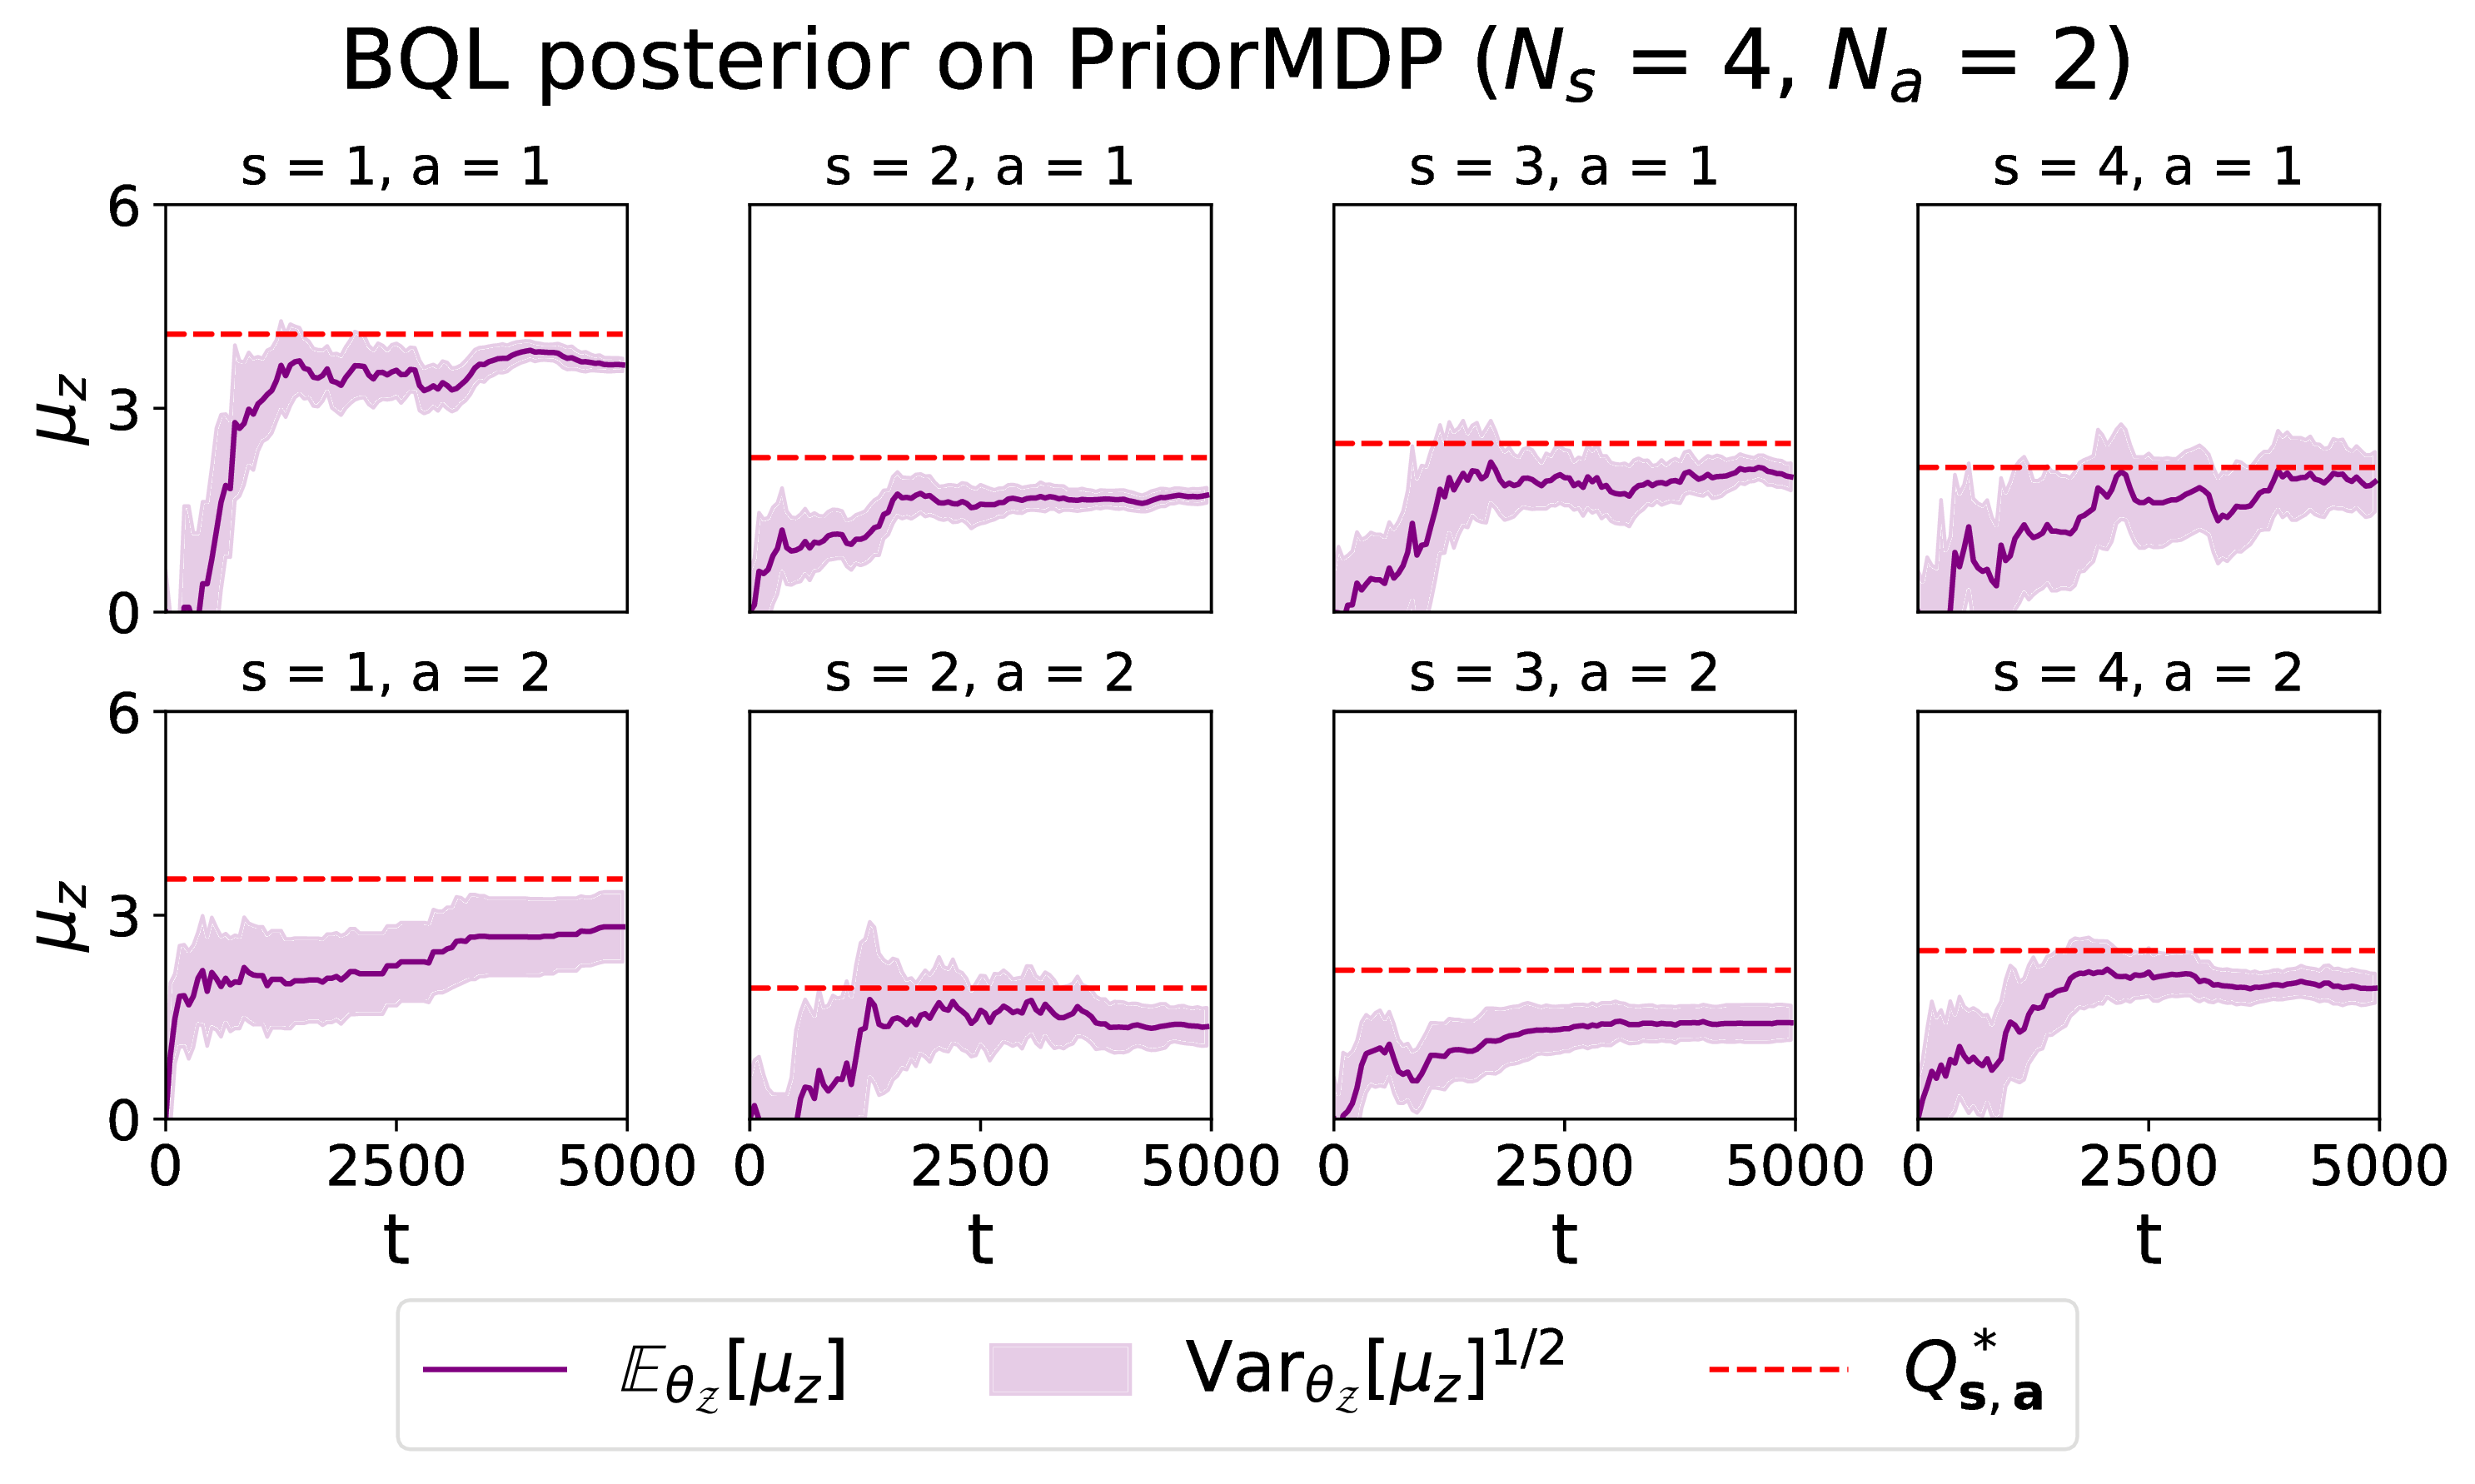
\includegraphics[width=\linewidth]{img/bql-0_0-4_0-3_0-3_0-posterior-priormdp-4-2.pdf}
\end{subfigure}
\begin{subfigure}{0.34\textwidth}
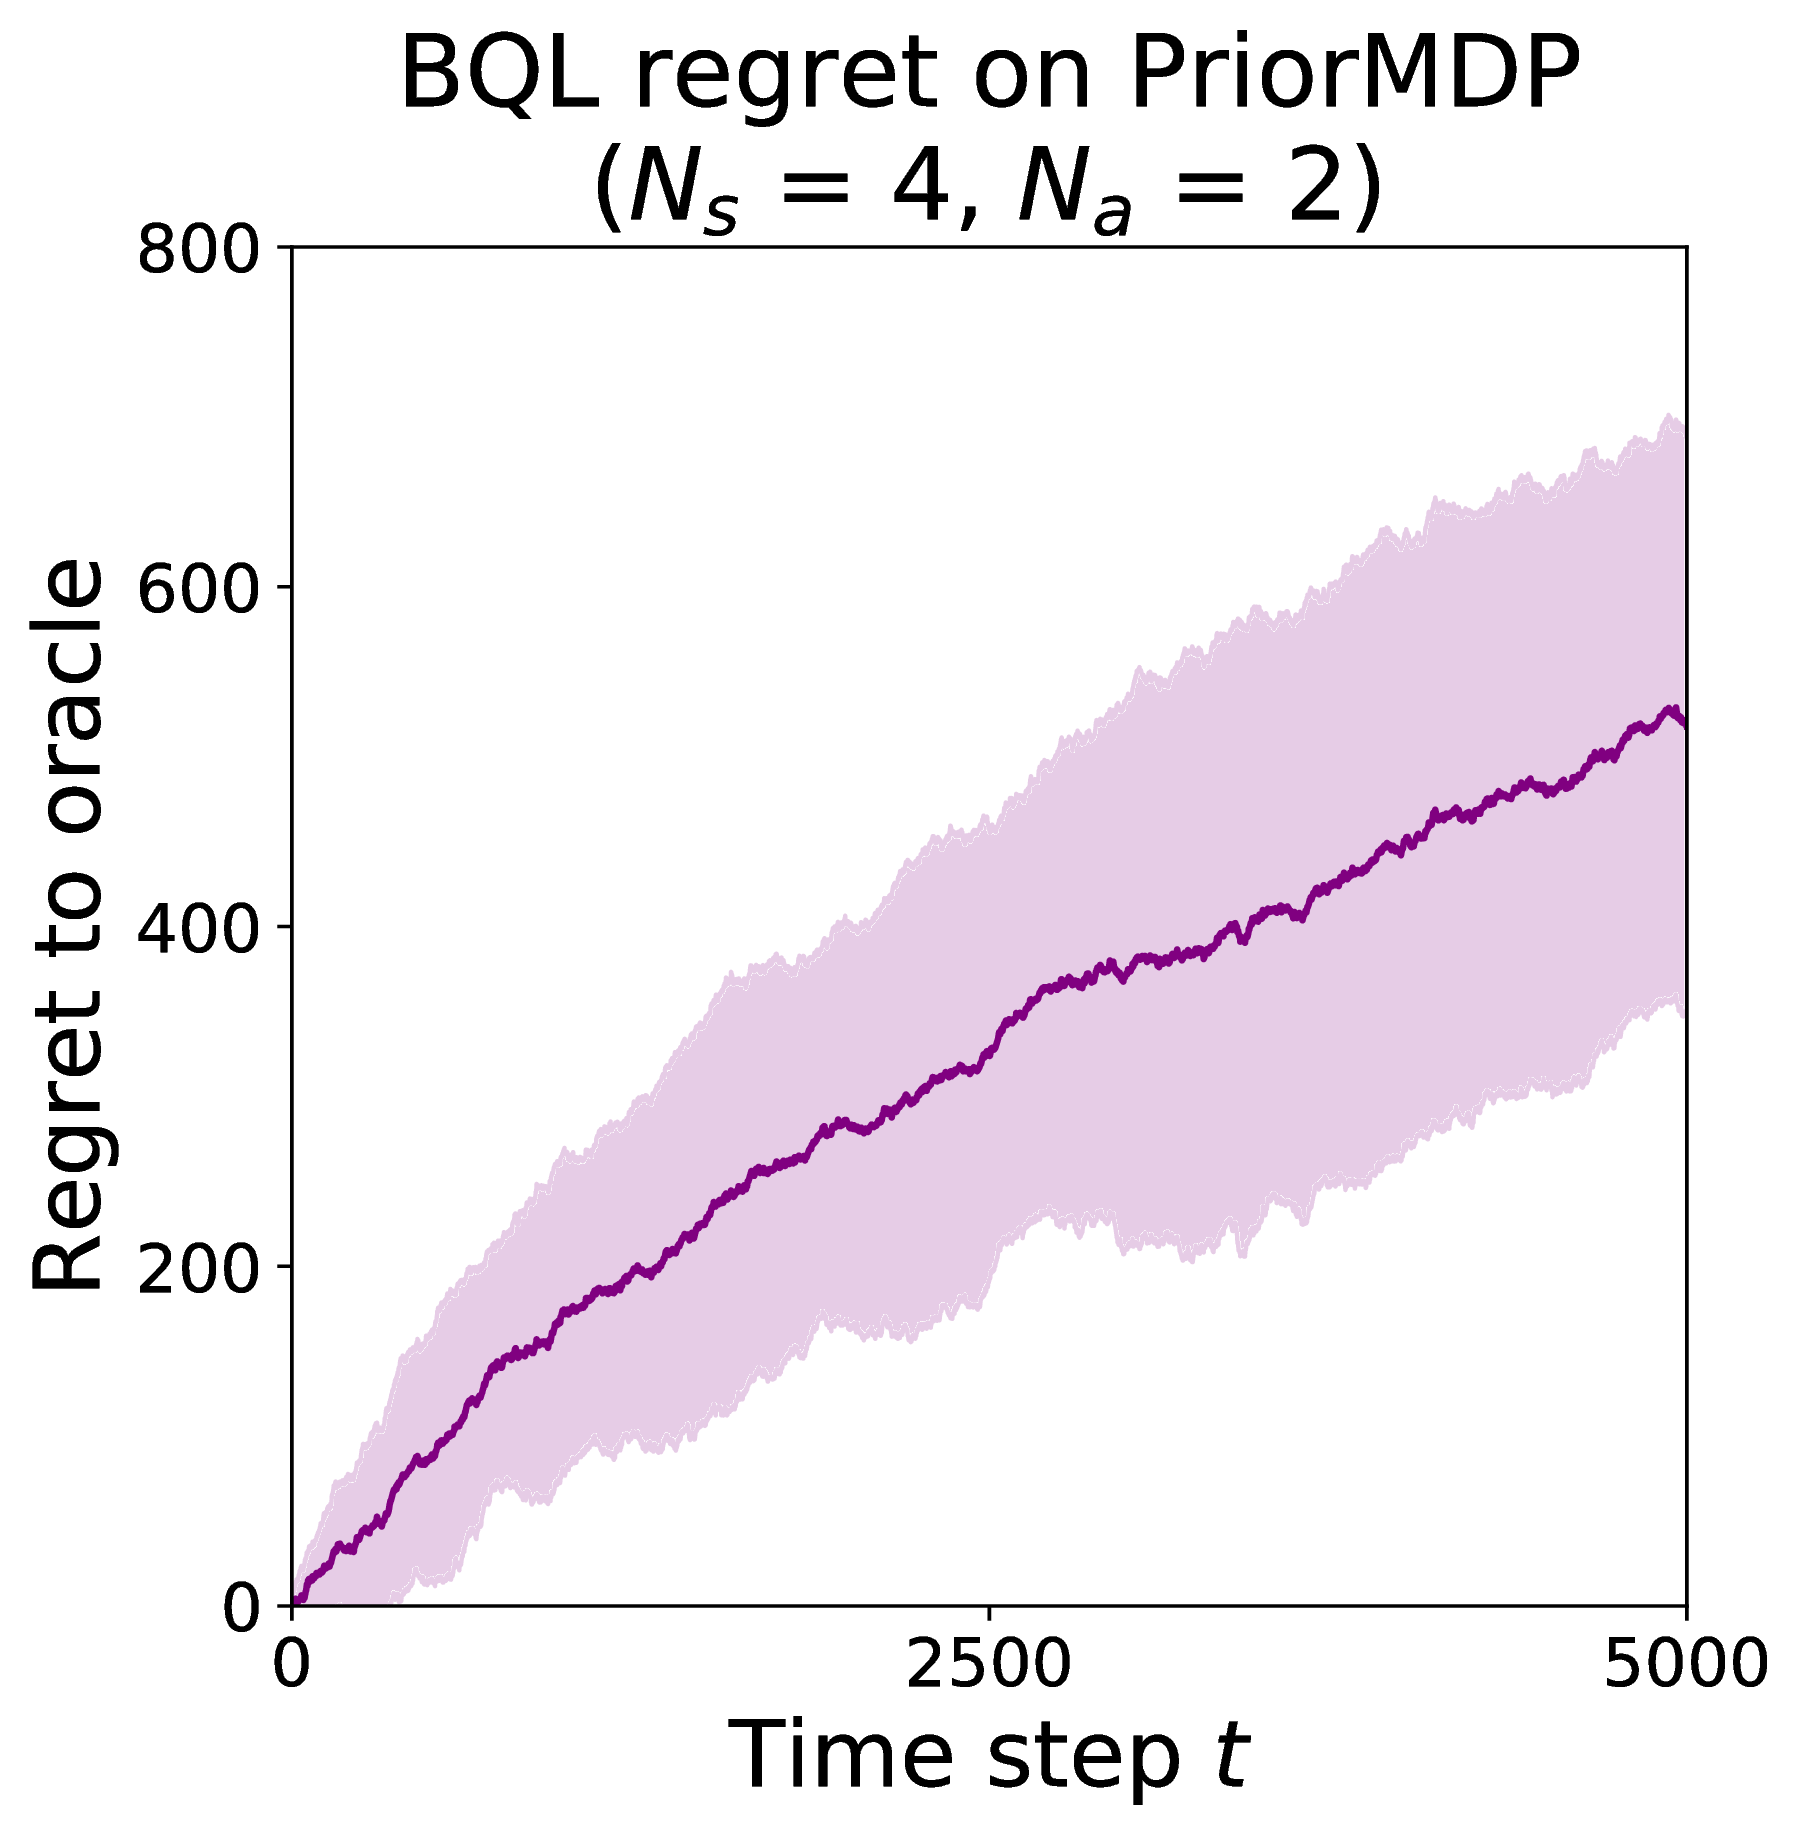
\includegraphics[width=\linewidth]{img/bql-0_0-4_0-3_0-3_0-regret-priormdp-4-2.pdf}~\\~\\
\end{subfigure}
\captionsetup{width=0.9\linewidth}
\caption{BQL posterior and regret on PriorMDP.}\label{bql_priormdp_visual}
\end{figure}

\begin{figure}[h!]
\centering
\begin{subfigure}{0.65\textwidth}
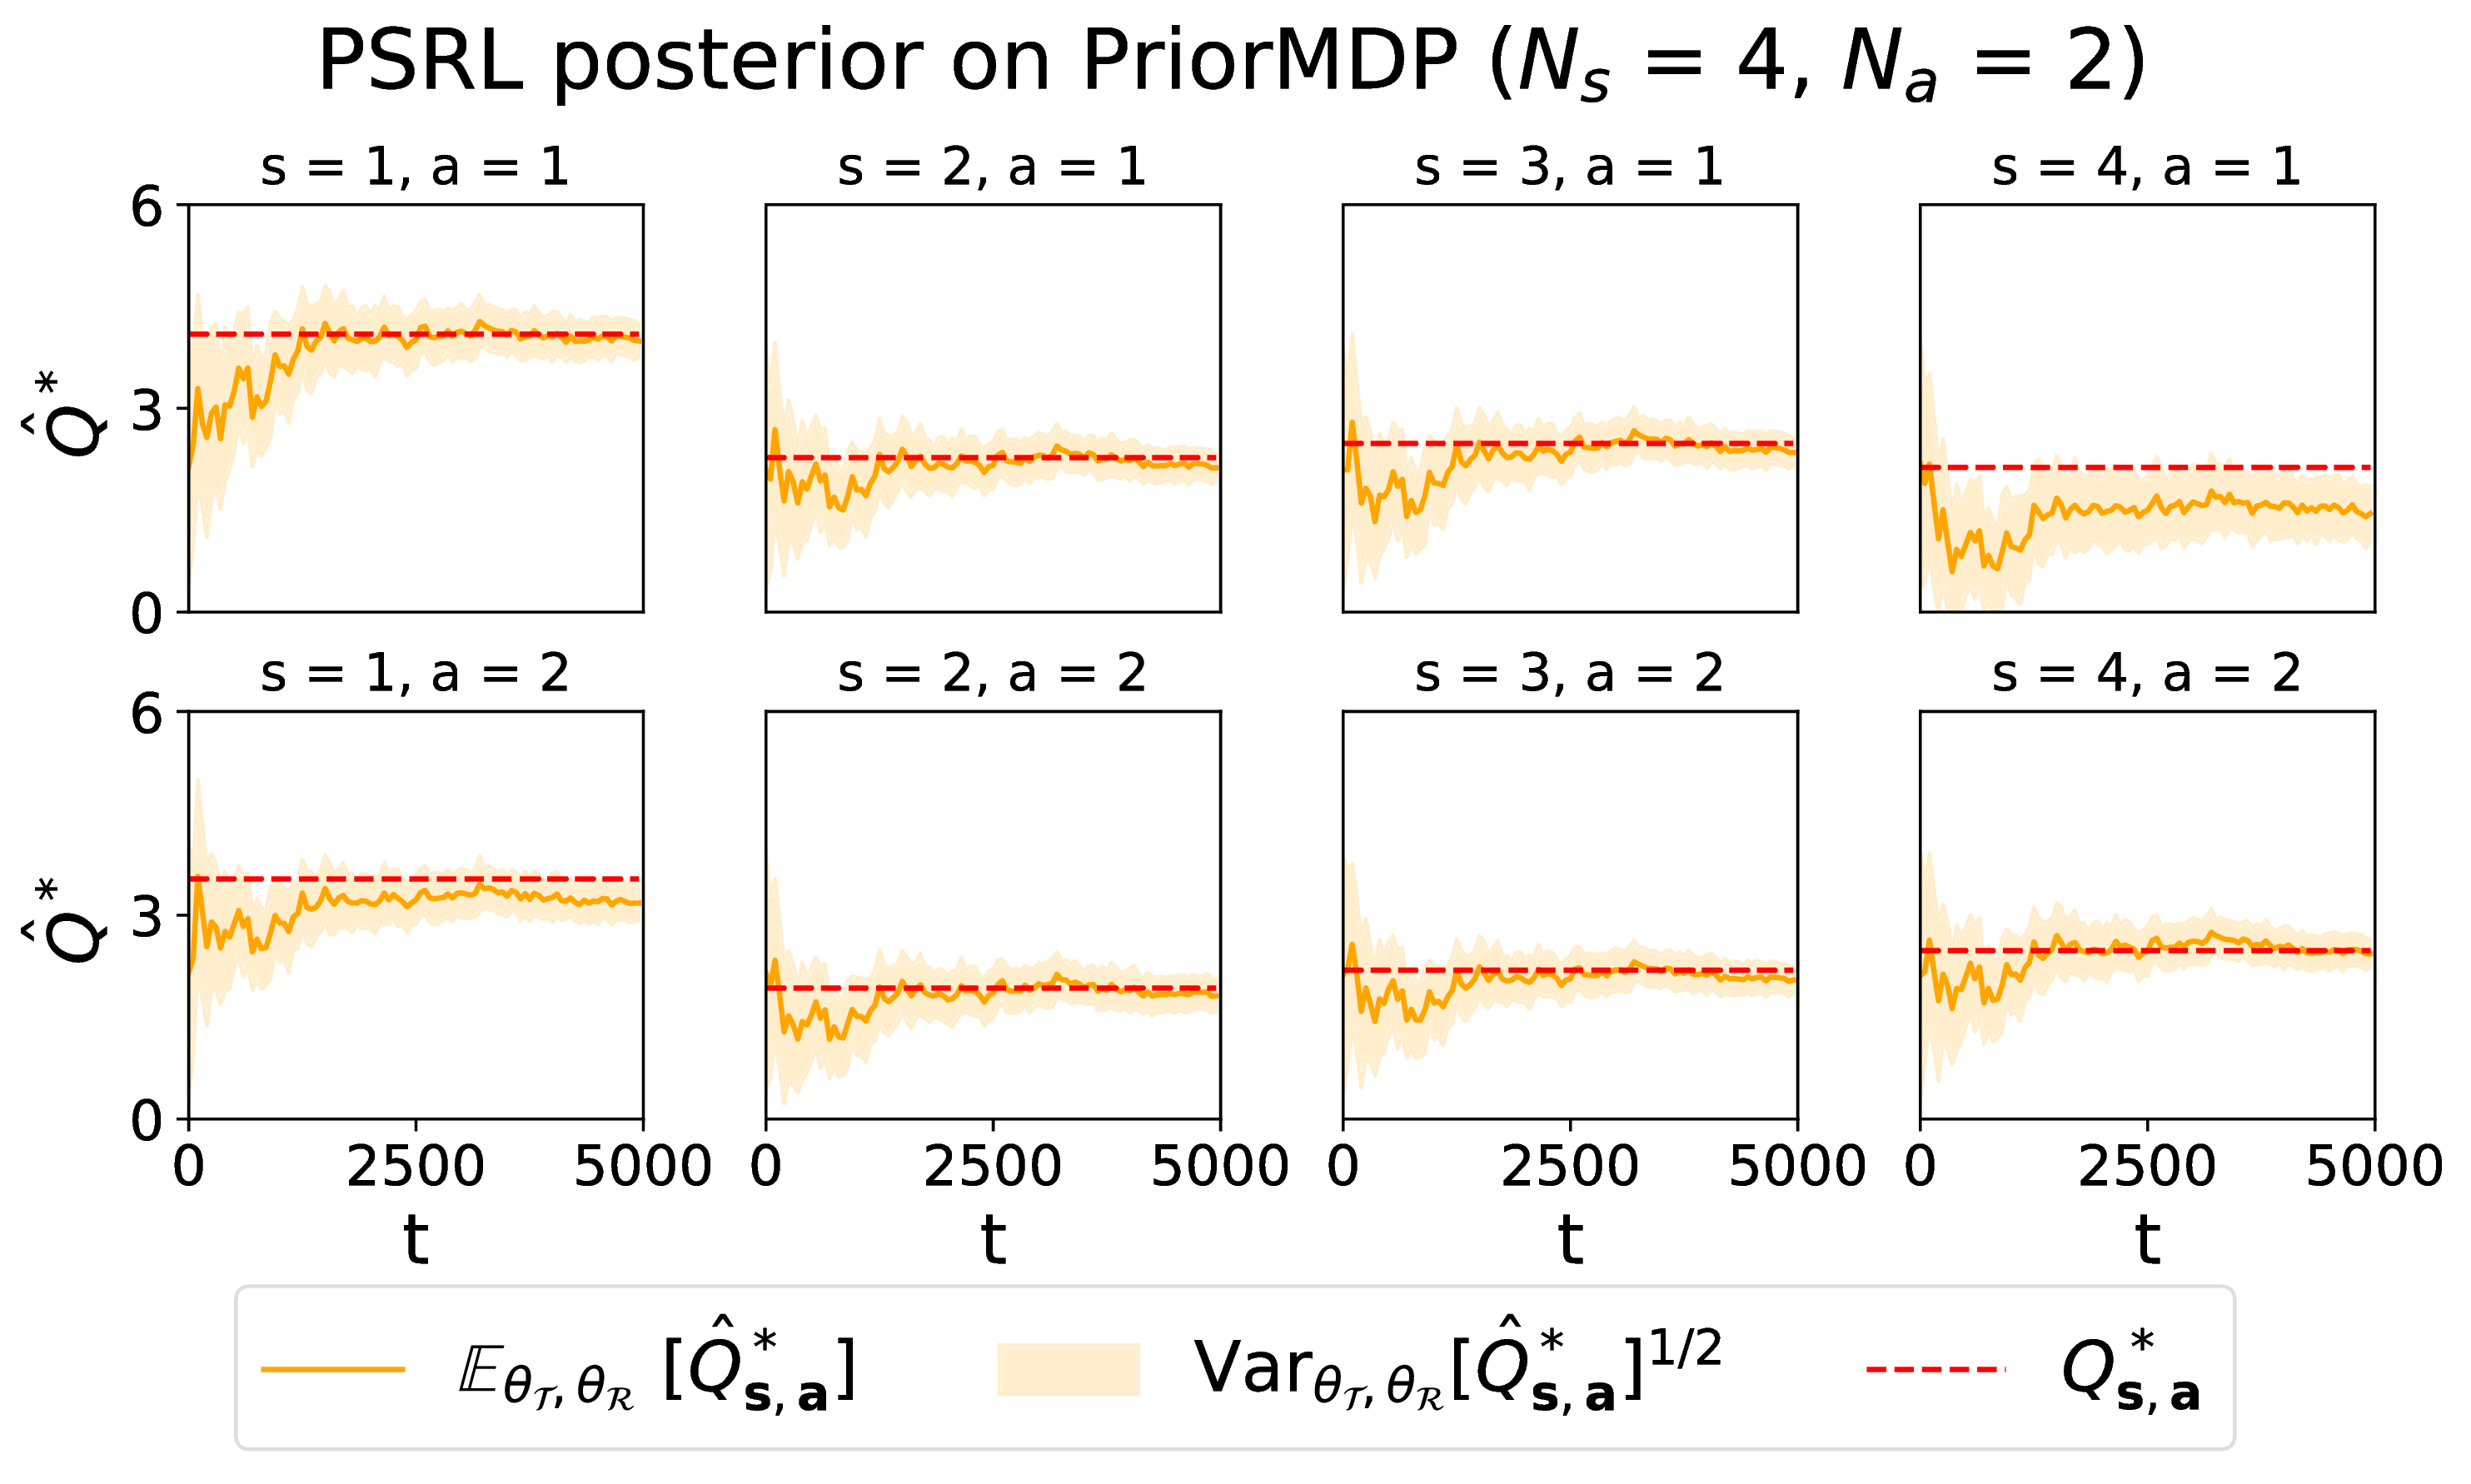
\includegraphics[width=\linewidth]{img/psrl-0_0-4_0-3_0-3_0-posterior-priormdp-4-2.pdf}
\end{subfigure}
\begin{subfigure}{0.34\textwidth}
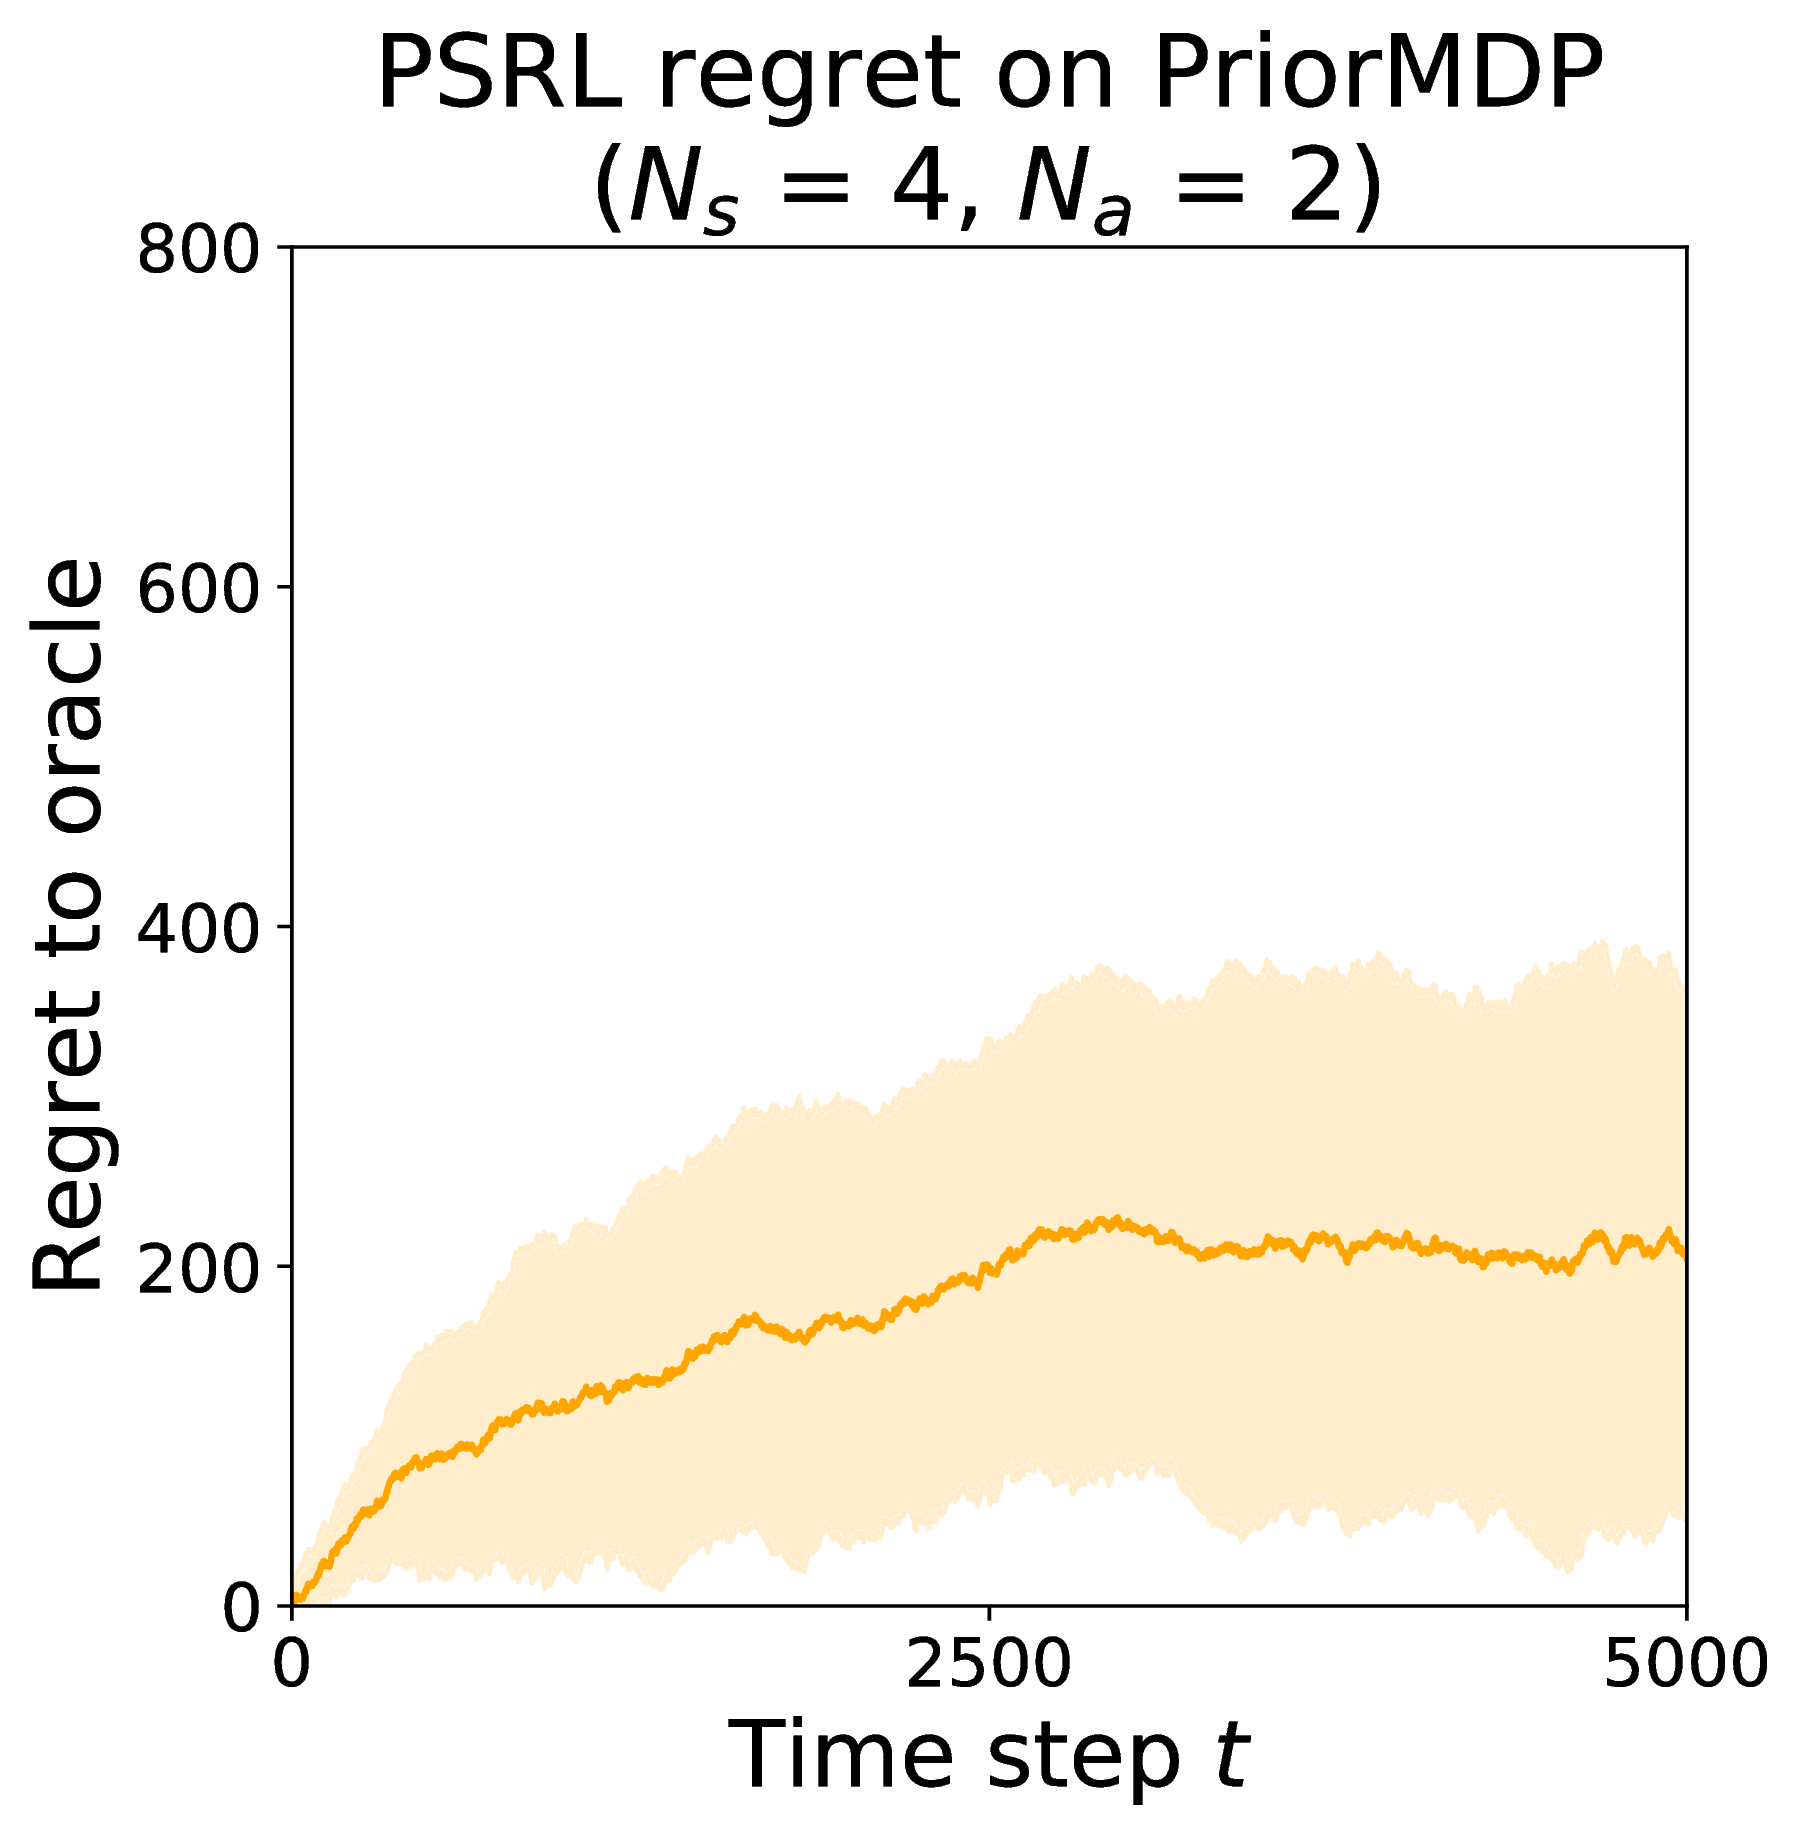
\includegraphics[width=\linewidth]{img/psrl-0_0-4_0-3_0-3_0-regret-priormdp-4-2.pdf}~\\~\\
\end{subfigure}
\captionsetup{width=0.9\linewidth}
\caption{PSRL posterior and regret on PriorMDP.}\label{psrl_priormdp_visual}
\end{figure}

\begin{figure}[h!]
\centering
\begin{subfigure}{0.65\textwidth}
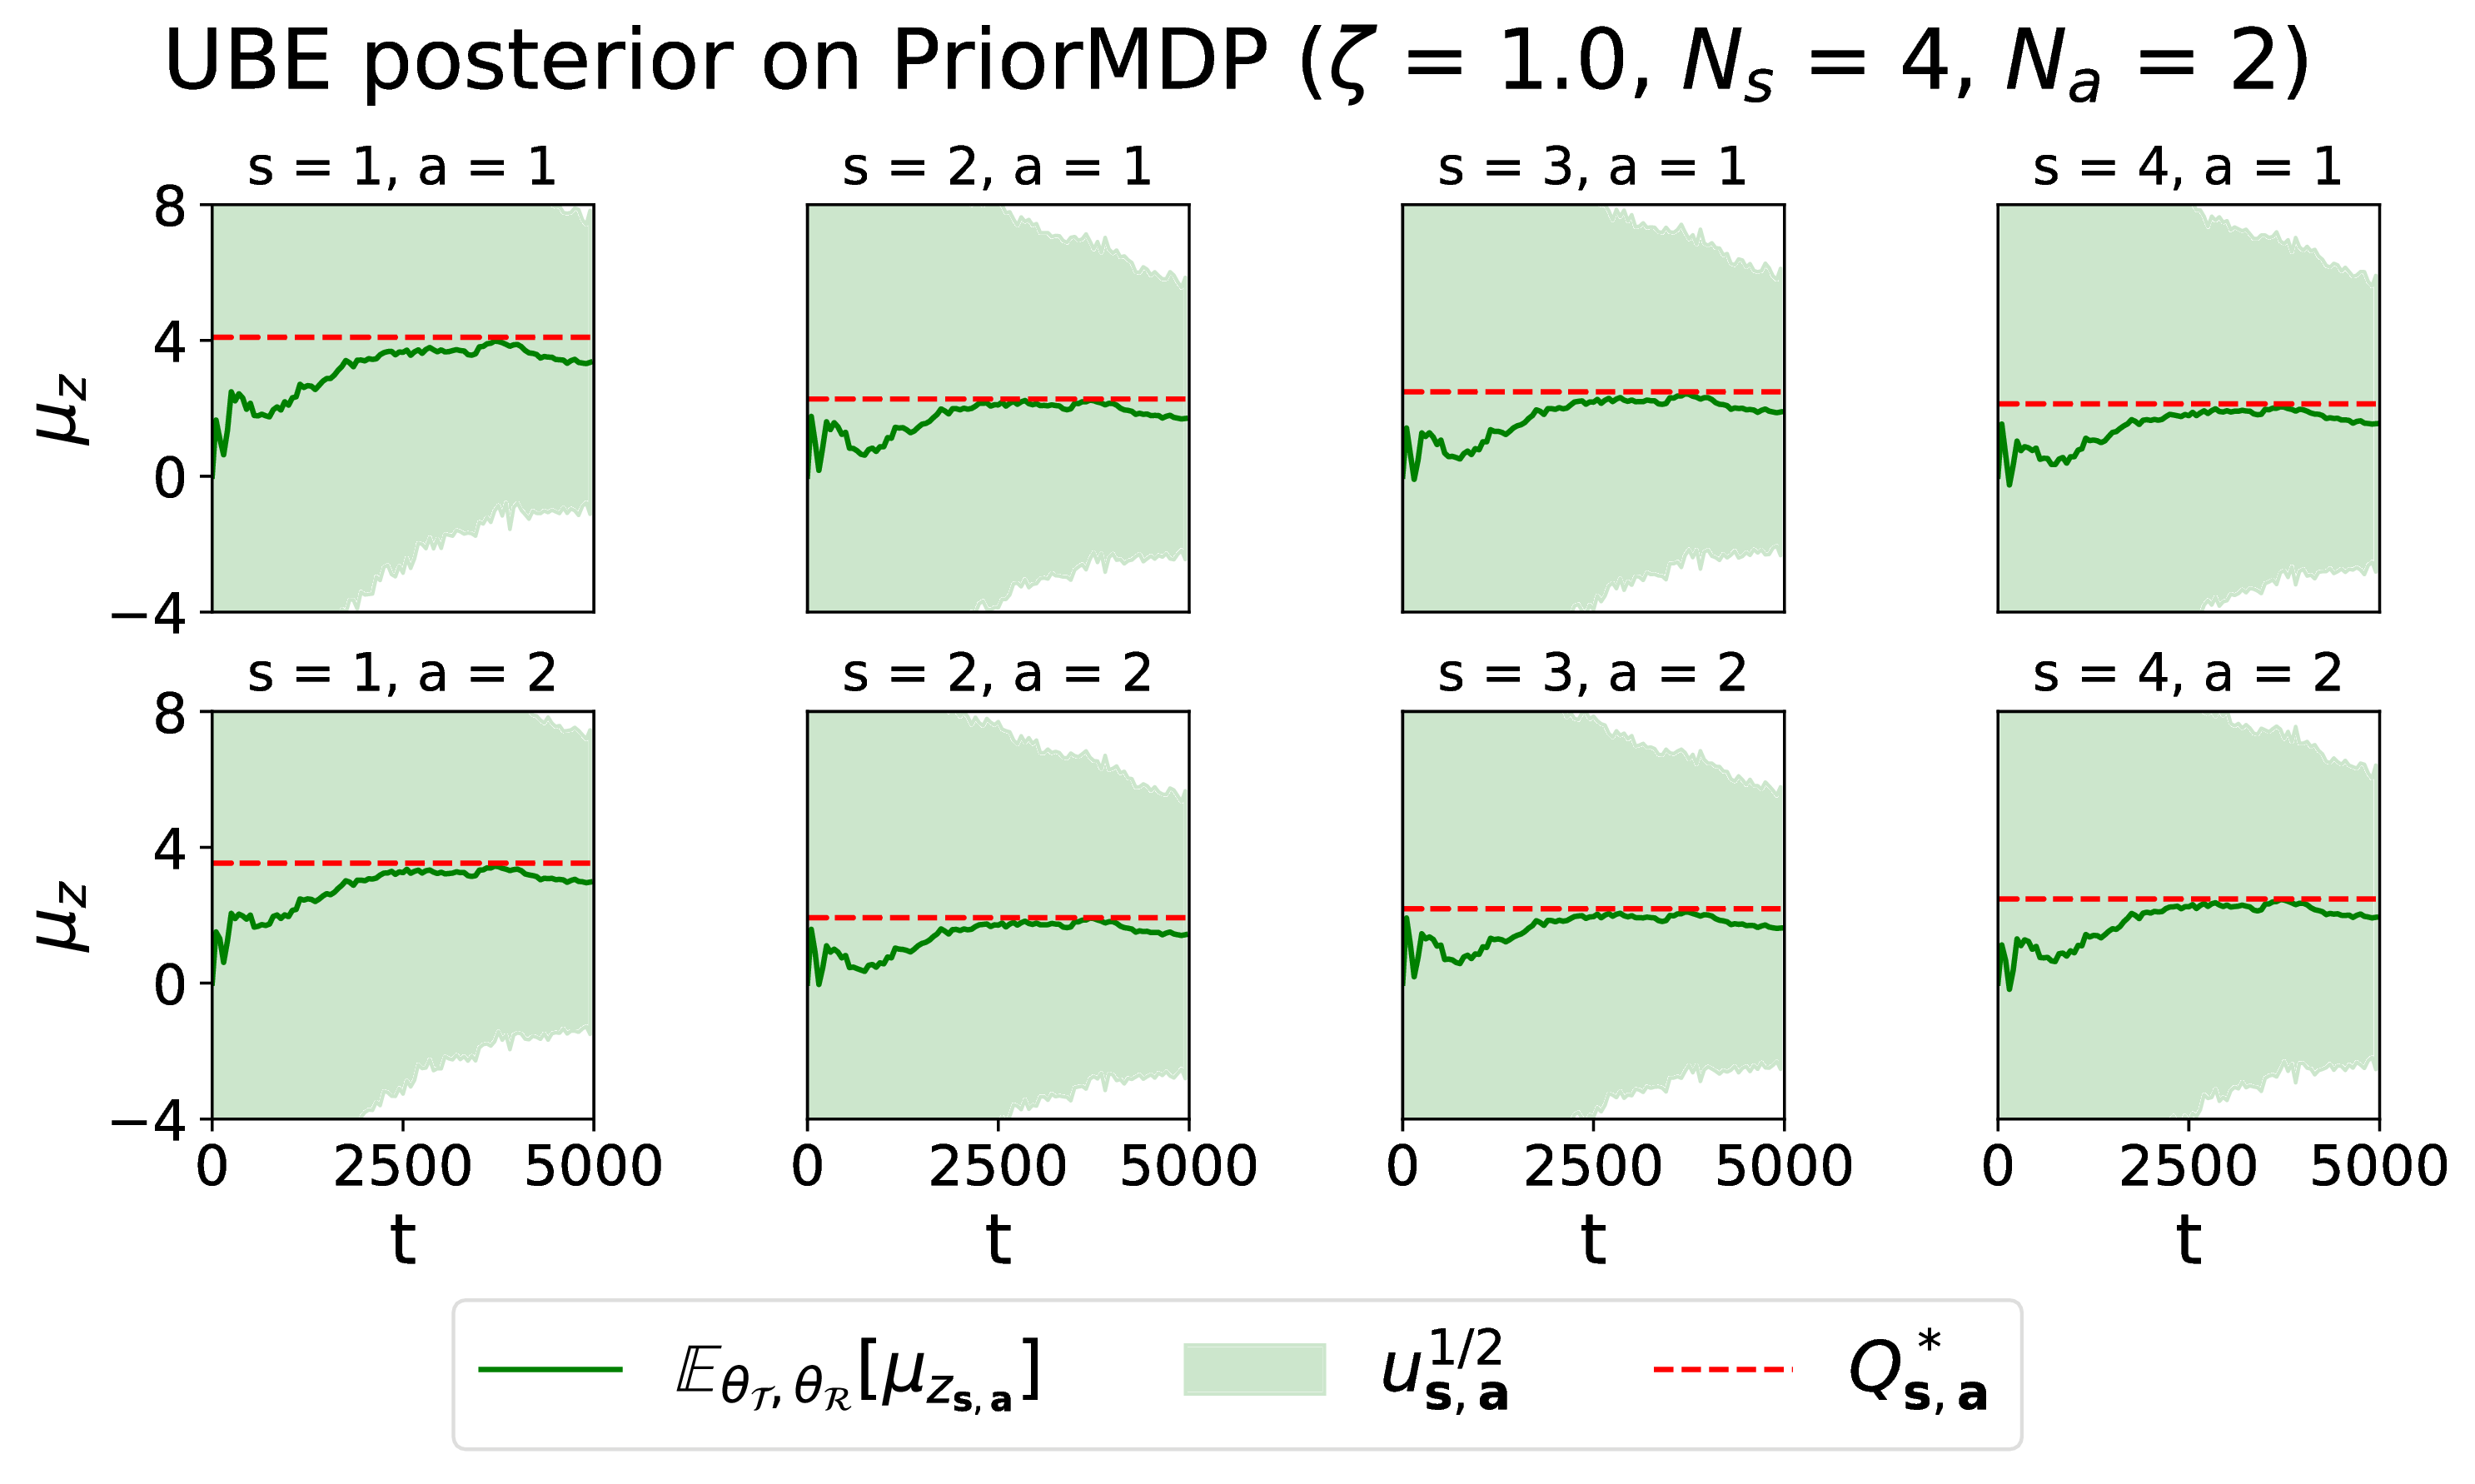
\includegraphics[width=\linewidth]{img/ube-0_0-4_0-3_0-3_0-1_0-posterior-priormdp-4-2.pdf}
\end{subfigure}
\begin{subfigure}{0.34\textwidth}
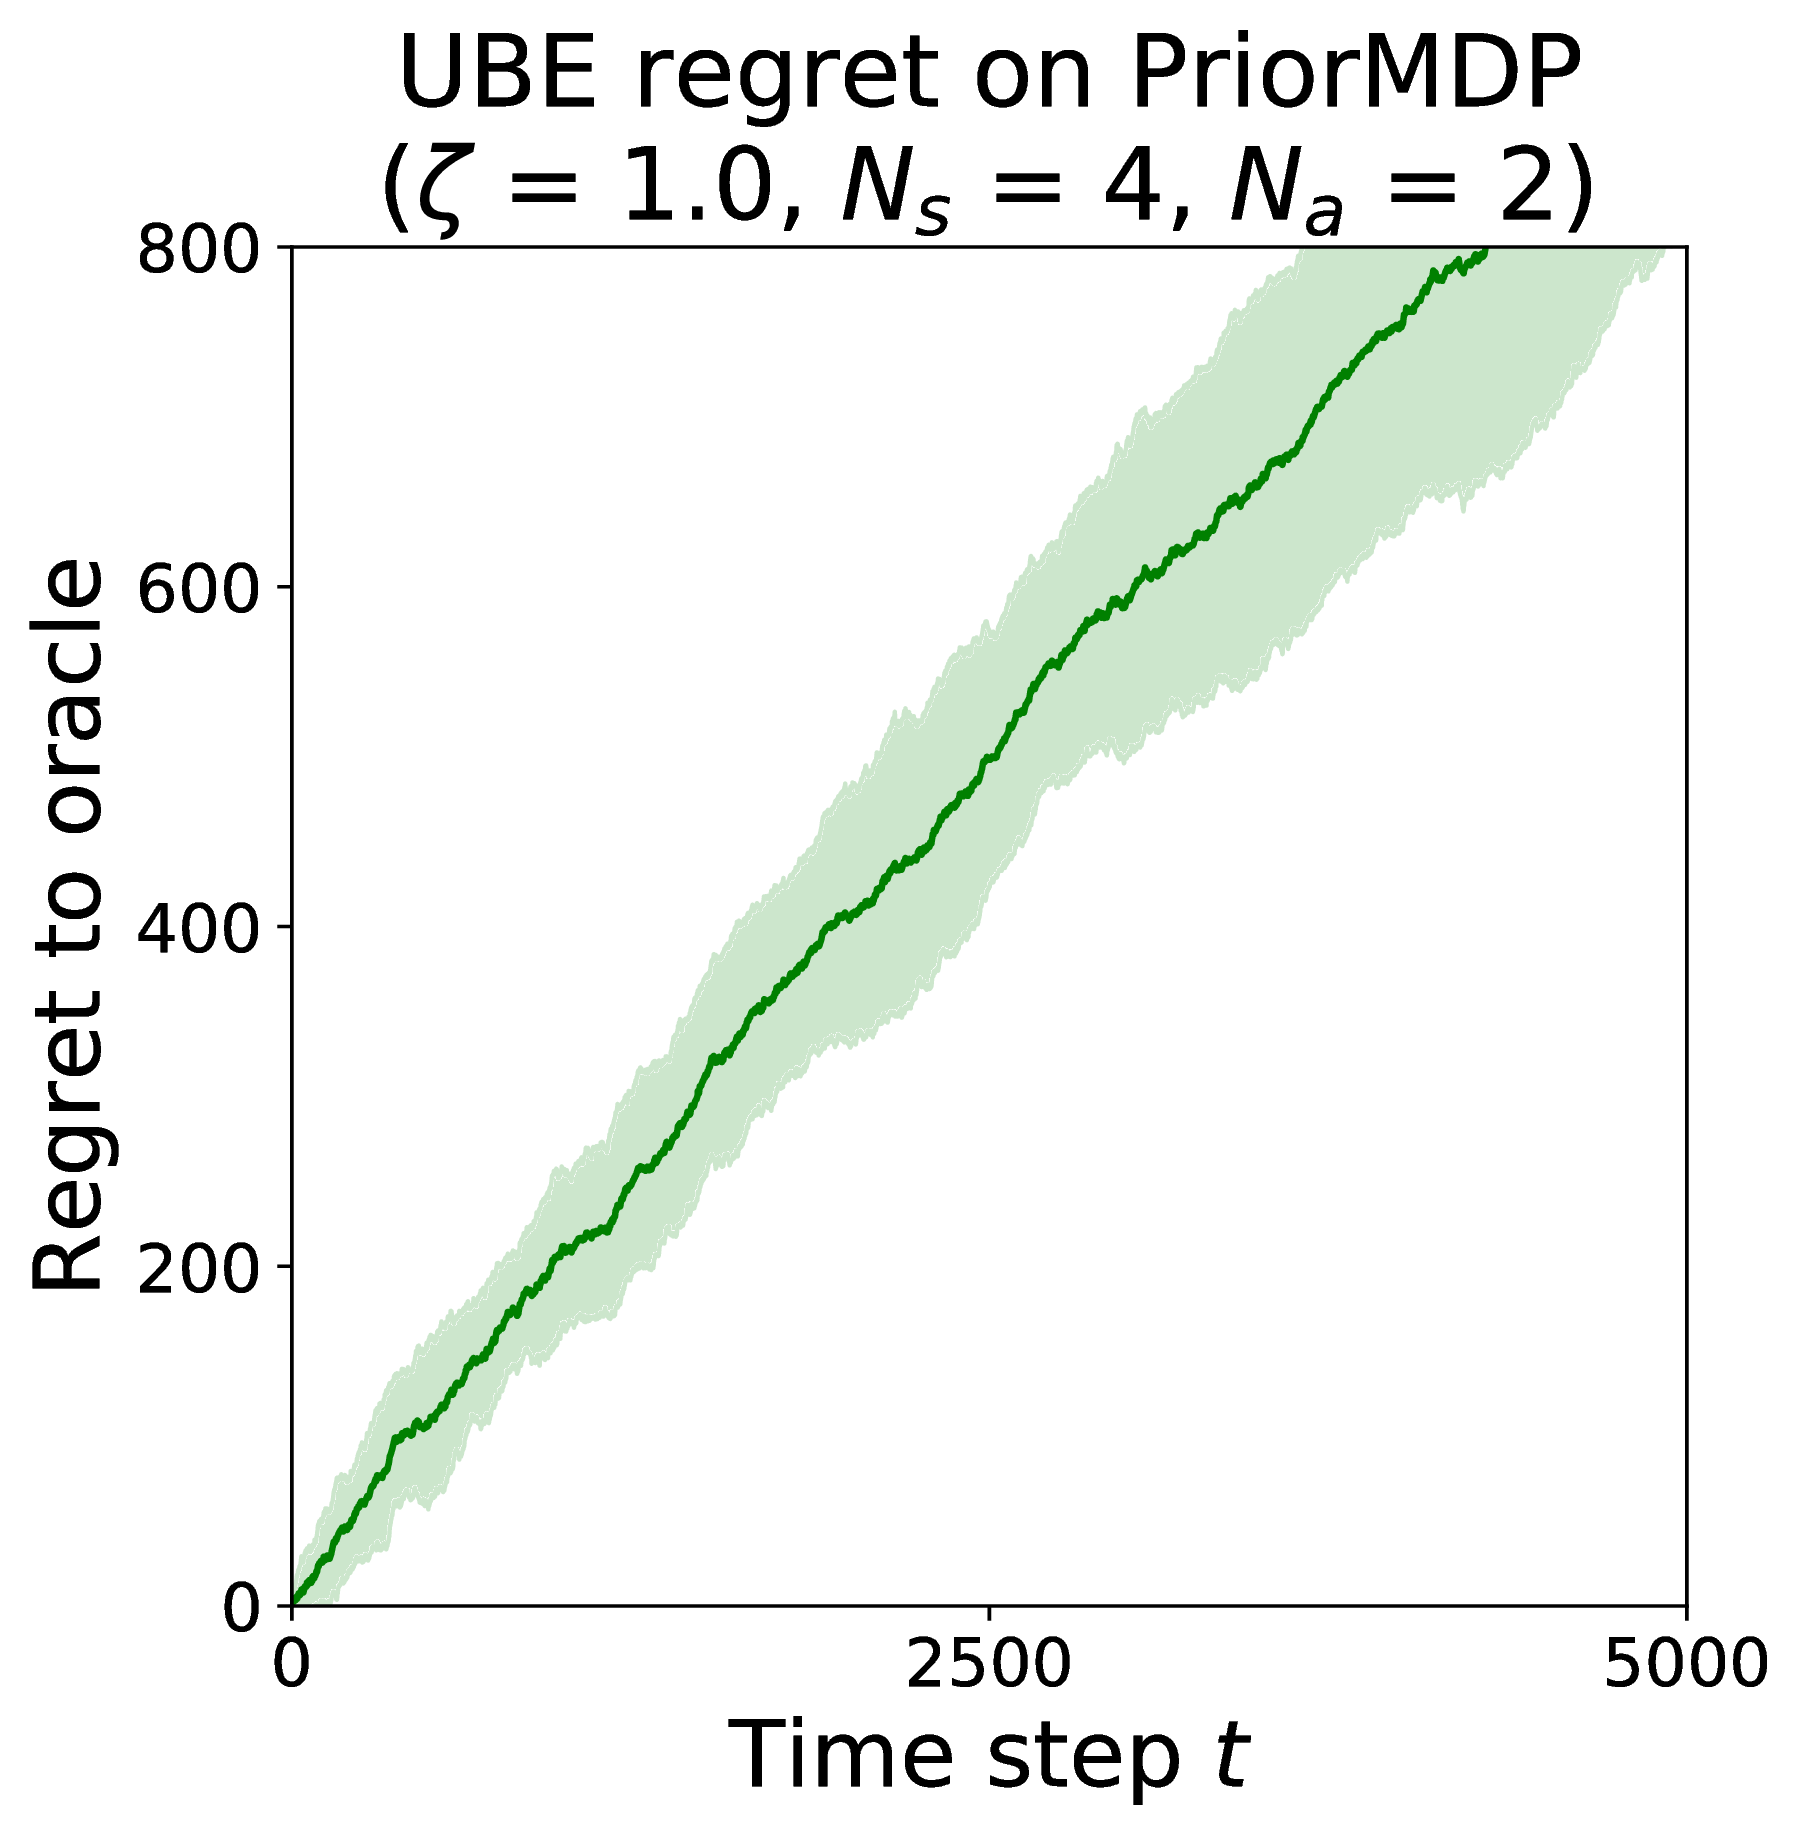
\includegraphics[width=\linewidth]{img/ube-0_0-4_0-3_0-3_0-1_0-regret-priormdp-4-2.pdf}~\\~\\
\end{subfigure}
\captionsetup{width=0.9\linewidth}
\caption{UBE posterior and regret on PriorMDP.}\label{ube_priormdp_visual1}
\end{figure}

\begin{figure}[h!]
\centering
\begin{subfigure}{0.65\textwidth}
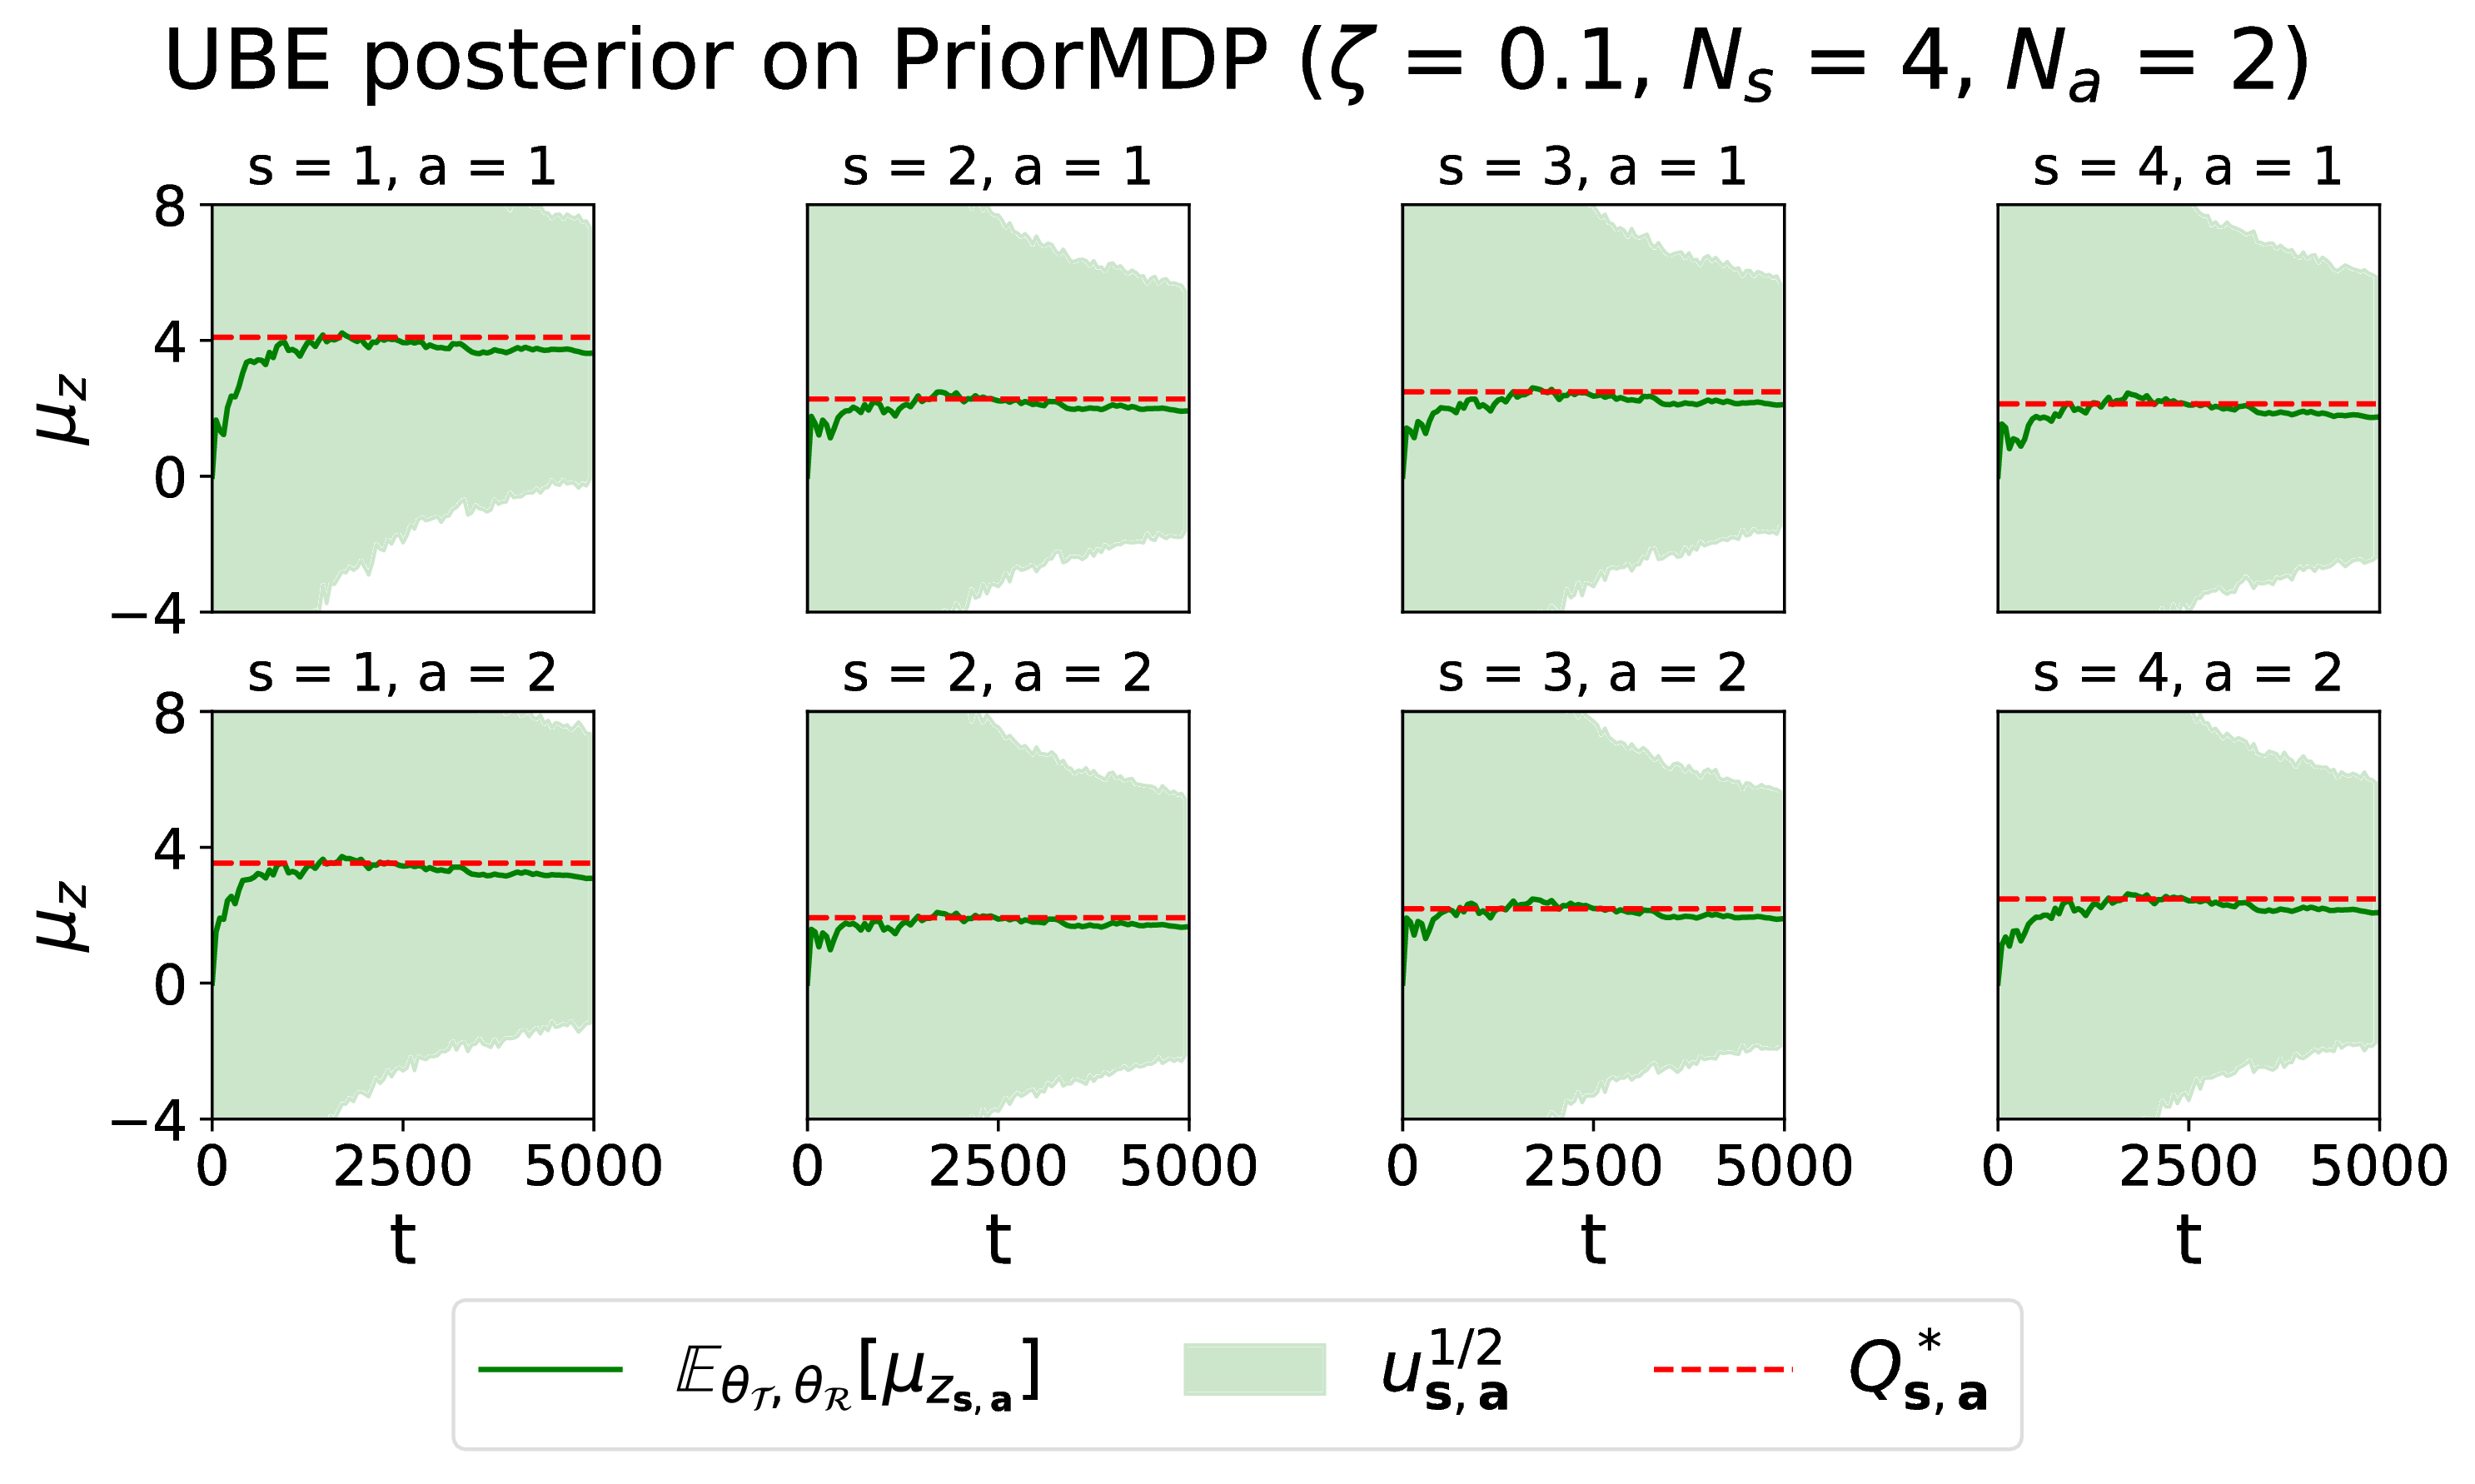
\includegraphics[width=\linewidth]{img/ube-0_0-4_0-3_0-3_0-0_1-posterior-priormdp-4-2.pdf}
\end{subfigure}
\begin{subfigure}{0.34\textwidth}
\includegraphics[width=\linewidth]{img/ube-0_0-4_0-3_0-3_0-0_1-regret-priormdp-4-2.pdf}~\\~\\
\end{subfigure}
\captionsetup{width=0.9\linewidth}
\caption{UBE posterior and regret on PriorMDP.}\label{ube_priormdp_visual1}
\end{figure}

\begin{figure}[h!]
\centering
\begin{subfigure}{0.65\textwidth}
\includegraphics[width=\linewidth]{img/mm-0_0-4_0-3_0-3_0-1_0-posterior-priormdp-4-2.pdf}
\end{subfigure}
\begin{subfigure}{0.34\textwidth}
\includegraphics[width=\linewidth]{img/mm-0_0-4_0-3_0-3_0-1_0-regret-priormdp-4-2.pdf}~\\~\\
\end{subfigure}
\captionsetup{width=0.9\linewidth}
\caption{MM posterior and regret on PriorMDP.}\label{mm_priormdp_visual}
\end{figure}


\clearpage

\begin{figure}[h!]
\centering
\begin{subfigure}{1.0\textwidth}
\includegraphics[width=\linewidth]{img/bql-0_0-4_0-3_0-3_0-scatter-priormdp-4-2-1000.pdf}
\end{subfigure}\\
~\\
~\\
\begin{subfigure}{1.0\textwidth}
\includegraphics[width=\linewidth]{img/psrl-0_0-4_0-3_0-3_0-scatter-priormdp-4-2-1000.pdf}
\end{subfigure}\\
~\\
~\\
\begin{subfigure}{1.0\textwidth}
\includegraphics[width=\linewidth]{img/ube-0_0-4_0-3_0-3_0-0_1-scatter-priormdp-4-2-1000.pdf}
\end{subfigure}\\
~\\
~\\
\begin{subfigure}{1.0\textwidth}
\includegraphics[width=\linewidth]{img/mm-0_0-4_0-3_0-3_0-1_0-scatter-priormdp-4-2-1000.pdf}
\end{subfigure}\\
\captionsetup{width=0.9\linewidth}
\caption{Correlation plots for PriorMDP at time step $t = 1,000$.}\label{correlations_priormdp_500}
\end{figure}

\begin{figure}[h!]
\centering
\begin{subfigure}{1.0\textwidth}
\includegraphics[width=\linewidth]{img/bql-0_0-4_0-3_0-3_0-scatter-priormdp-4-2-5000.pdf}
\end{subfigure}\\
~\\
~\\
\begin{subfigure}{1.0\textwidth}
\includegraphics[width=\linewidth]{img/psrl-0_0-4_0-3_0-3_0-scatter-priormdp-4-2-5000.pdf}
\end{subfigure}\\
~\\
~\\
\begin{subfigure}{1.0\textwidth}
\includegraphics[width=\linewidth]{img/ube-0_0-4_0-3_0-3_0-0_1-scatter-priormdp-4-2-5000.pdf}
\end{subfigure}\\
~\\
~\\
\begin{subfigure}{1.0\textwidth}
\includegraphics[width=\linewidth]{img/mm-0_0-4_0-3_0-3_0-1_0-scatter-priormdp-4-2-5000.pdf}
\end{subfigure}\\
\captionsetup{width=0.9\linewidth}
\caption{Correlation plots for PriorMDP at time step $t = 5,000$.}\label{correlations_priormdp_2500}
\end{figure}

\end{appendices}

\end{document}
